\documentclass[10pt]{amsart}
\usepackage[a4paper,margin=23mm]{geometry}
\usepackage{amsmath,amssymb,amsthm,mathtools,hyperref,graphicx,xspace,letltxmacro,xpatch}
\usepackage[english]{babel}
\newtheorem{theo}{Theorem}[section]
\newtheorem{lemm}[theo]{Lemma}\newtheorem{prop}[theo]{Proposition}\newtheorem{coro}[theo]{Corollary}\newtheorem{conj}[theo]{Conjecture}
\theoremstyle{definition}\newtheorem{defi}[theo]{Definition}\newtheorem{rema}[theo]{Remark}\newtheorem{exam}[theo]{Example}\newtheorem{exem}[theo]{Example}\newtheorem{nota}[theo]{Notation}
\newcommand{\ie}{i.e.}\newcommand{\eg}{e.g.}\newcommand{\resp}{resp.}\newcommand{\skpt}{\par\smallskip\noindent}
\emergencystretch=3em\pagestyle{plain}
%~Mouliné par MaN_auto v.0.33.4 2025-03-26 10:25:27

\usepackage[normalem]{ulem}
\usepackage{mathrsfs}
\usepackage[inline]{enumitem}
\usepackage{stackengine}
\usepackage{graphicx}
\usepackage{xcolor}
\usepackage{import}






\newcommand{\fa}{\forall\,}
\newcommand{\nin}{\not\in}
\newcommand{\eps}{\varepsilon}
\newcommand{\defeq}{\doteqdot}
\newcommand{\ct}{r}
\newcommand{\fft}{\tau}
\newcommand{\curv}{\kappa}


\newcommand{\deh}{\mathrm{d}}
\newcommand{\st}{\ \text{s.t.}\ }




\newcommand{\intr}[1]{\mathrm{int}\,#1}

\newcommand{\cl}[1]{\mathrm{cl}\,#1}
\DeclareMathOperator{\diam}{diam}
\newcommand{\const}{C_\#}
\newcommand{\inv}{^{-1}}
\newcommand{\unstable}{\text{u}}
\newcommand{\stable}{\text{s}}



\newcommand{\ifrac}[2]{#1/#2}

\newcommand{\mes}{{\mathrm{mes}}}
\newcommand{\crit}{\mathrm{C}}
\newcommand{\ctc}{\ct_\crit}
\newcommand{\xc}{x_\crit}

\newcommand{\fixw}{\mathrm{F}}
\newcommand{\bd}{\mathbf{d}}


\newcommand{\naturals}{\mathbb{N}}
\newcommand{\integers}{\mathbb{Z}}
\newcommand{\reals}{\mathbb{R}}
\newcommand{\bR}{\mathbb{R}}
\newcommand{\bZ}{\mathbb{Z}}
\newcommand{\bN}{\mathbb{N}}
\newcommand{\hhs}{\mathbb{S}}
\newcommand{\LC}{\mathbb{K}}
\newcommand{\homo}{\mathbb{H}}

\newcommand{\Rect}{{\mathfrak{R}}}
\newcommand{\fka}{\mathfrak{a}}
\newcommand{\fkN}{\mathfrak{N}}
\newcommand{\fkb}{\mathfrak{b}}

\newcommand{\cB}{\mathcal{B}}
\newcommand{\cF}{\mathcal{F}}
\newcommand{\cK}{\mathcal{K}}
\newcommand{\cI}{\mathcal{I}}
\newcommand{\cO}{\mathcal{O}}
\newcommand{\cR}{\mathcal{R}}
\newcommand{\cE}{\mathcal E}
\newcommand{\cEs}{\mathcal E^{*}}

\newcommand{\cpar}{\mathcal{R}}
\newcommand{\pslope}{\mathcal{B}}
\newcommand{\cslope}{\mathcal{V}}
\newcommand{\tang}{\mathcal{T}}
\newcommand{\tangu}{\mathcal{T}^1}
\newcommand{\cm}{\mathcal{F}}
\newcommand{\cell}{\mathcal{D}}
\newcommand{\hol}{\mathcal{H}}
\newcommand{\csp}{\mathcal{M}}
\newcommand{\cmp}{\hat\cm}


\newcommand{\cone}{\mathcal{C}}
\newcommand{\cspl}[1]{\csp_{\ge\,#1}}
\newcommand{\cspu}[1]{\csp_{\le\,#1}}
\newcommand{\cspi}{\widehat{\csp}}
\newcommand{\cspil}[1]{\widehat{\csp}_{\ge\,#1}}
\newcommand{\cspiu}[1]{\widehat{\csp}_{\le\,#1}}
\newcommand{\csps}{\csp_\text{S}}

\newcommand{\brA}{\bar{A}}
\newcommand{\brC}{\bar{C}}
\newcommand{\brrC}{\bar{\brC}}
\newcommand{\brrrC}{\bar{\brrC}}
\newcommand{\brn}{\bar{n}}
\newcommand{\brw}{\bar{w}}
\newcommand{\brW}{\overline{W}}
\newcommand{\brV}{\overline{V}}
\newcommand{\brx}{\bar{x}}
\newcommand{\breps}{\bar{\varepsilon}}
\newcommand{\brdelta}{\bar{\delta}}

\newcommand{\privateu}[1]{#1^*}
\newcommand{\privatel}[1]{#1_*}

\newcommand{\slope}{h}
\newcommand{\slopeb}{\mathfrak{h}}
\newcommand{\slopeu}{\privateu{\slope}}
\newcommand{\slopel}{\privatel{\slope}}
\newcommand{\ellu}{\privateu{\ell}}
\newcommand{\elll}{\privatel{\ell}}


\newcommand{\lboundary}{\partial^\text l}
\newcommand{\rboundary}{\partial^\text r}

\newcommand{\tcF}{\widetilde{\mathcal{F}}}
\newcommand{\tV}{\widetilde{V}}
\newcommand{\tW}{\widetilde{W}}

\newcommand{\matrixtt}[4]{\left(
\begin{array}{cc}#1&#2\\#3&#4
\end{array}\right)}
\newcommand{\vectt}[2]{\left(
\begin{array}{c}#1\\#2
\end{array}\right)}
\newcommand{\Hcomp}{H-\hskip0pt component}
\newcommand{\Hcomps}{H-\hskip0pt components}


\newcommand{\recoPrivate}{\mathrm{R}}
\newcommand{\reco}{{\cell^-_{\recoPrivate}}}
\newcommand{\backReco}{{\cell^+_{\recoPrivate}}}
\newcommand{\recoMp}{{\cell^\mp_{\recoPrivate}}}
\newcommand{\exph}{\Omega}

\newcommand{\invo}{\cI}
\newcommand{\flow}[1]{\Phi^{#1}}
\newcommand{\rflow}[1]{\bar\Phi^{#1}}
\newcommand{\rell}{\bar\ell}






\newcommand{\conep}{\bar\cone^+}
\newcommand{\conen}{\bar\cone^-}
\newcommand{\coneu}{\cone^\unstable}
\newcommand{\oconeu}{\mathring{\cone}^\unstable}
\newcommand{\cconeu}{\bar{\cone}^\unstable}
\newcommand{\cones}{\cone^\stable}
\newcommand{\ccones}{\bar\cone^\stable}
\newcommand{\ocones}{\mathring{\cone}^\stable}
\newcommand{\mconeu}{{\widetilde{\coneu}}}
\newcommand{\mcones}{{\widetilde{\cones}}}

\newcommand{\Ws}{W^{\stable}}
\newcommand{\Wu}{W^{\unstable}}
\newcommand{\dadm}[1]{\dadmPrivate^{#1}}
\newcommand{\dadmPrivate}{d\adm}
\newcommand{\deum}[1]{d\eum^{#1}}
\newcommand{\ds}{\dadmPrivate^{\stable}}
\newcommand{\du}{\dadmPrivate^{\unstable}}
\newcommand{\rs}{r_{\stable}}
\newcommand{\ru}{r_{\unstable}}

\newcommand{\eum}{_\text{E}}

\newcommand{\ppPrivate}[2]{#1^{#2}}
\newcommand{\prePrivate}[1]{\ppPrivate{#1}{-}}
\newcommand{\postPrivate}[1]{\ppPrivate{#1}{+}}
\newcommand{\prv}{\prePrivate{\bar v}}
\newcommand{\pov}{\postPrivate{\bar v}}
\newcommand{\prs}{\prePrivate{s}}
\newcommand{\pos}{\postPrivate{s}}
\newcommand{\prz}{\prePrivate{z}}
\newcommand{\poz}{\postPrivate{z}}
\newcommand{\prpslope}{\prePrivate{\pslope}}
\newcommand{\popslope}{\postPrivate{\pslope}}

\newcommand{\singPrivate}{\mathcal{S}}
\newcommand{\sing}[1]{\singPrivate^{#1}}
\newcommand{\singp}[1]{\hat{\singPrivate}^{#1}}
\newcommand{\hsing}[1]{{\singPrivate}_\homo^{#1}}
\newcommand{\hsingp}[1]{\hat{\singPrivate}_\homo^{#1}}

\newcommand{\singReco}{\singPrivate_{\recoPrivate}}
\newcommand{\singBoth}{\singPrivate^\pm}
\newcommand{\singForward}[1]{\singPrivate^+_{#1}}
\newcommand{\singBackward}[1]{\singPrivate^-_{#1}}

\newcommand{\singt}[1]{\tilde{\singPrivate}^{#1}}
\newcommand{\singr}[1]{\sing{#1}_*}



\newcommand{\cc}{\hat Q}
\newcommand{\cch}{\hat Q^{\mathbb{H}}}
\newcommand{\ccseq}[1]{\privSeq\cc{#1}}
\newcommand{\xseq}[1]{\privSeq x{#1}}
\newcommand{\indTuple}{\bar\indCell}

\newcommand{\admiss}{admissible}


\newcommand{\kreg}{K^\text{reg}}
\newcommand{\zreg}{\cL^\text{reg}}
\newcommand{\ckreg}{\mathcal{K}^\text{reg}}
\newcommand{\ckregp}{\hat{\mathcal{K}}^\text{reg}}
\newcommand{\hkreg}{\hat{K}^\text{reg}}
\newcommand{\hzreg}{\hat{\cL}^\text{reg}}
\newcommand{\kregp}{\hkreg}


\newcommand{\llw}{\stackunder[1.2pt]{$w$}{\rule{.8ex}{.075ex}}}


\newcommand{\law}[1]{\omega_{#1}}

\newcommand{\lawc}{\law{\#}}

\newcommand{\pme}{_\textup{p}}
\newcommand{\adm}{_{\alpha^{+}}}
\newcommand{\adms}{_{\alpha^{-}}}
\newcommand{\admPm}{_{\alpha^{\pm}}}
\newcommand{\admName}{\alpha^{+}}
\newcommand{\admNamePm}{\alpha^{\pm}}
\newcommand{\admNameM}{\alpha^{-}}
\newcommand{\aum}{_{*}}
\newcommand{\auum}{_{**}}
\newcommand{\admFunc}{\alpha^{+}}
\newcommand{\admFuncPm}{\alpha^{\pm}}
\newcommand\admParam[1]{
\ifnum0=#1\relax
\alpha_0
\else
\ifnum1=#1\relax
\alpha_1\fi\fi}
\newcommand{\Np}{\hat N}
\newcommand{\cL}{\mathcal{L}}

\newcommand{\Leb}{\textup{Leb}}

\newcommand{\cQ}{\mathcal{Q}}
\newcommand{\cU}{\mathcal{U}}
\newcommand{\cV}{\mathbb{V}}


\newcommand{\indCell}{\nu}
\newcommand{\redCell}{{\indCell^*}}
\newcommand{\multPrivate}{\mathcal{X}}
\newcommand{\mult}[1]{\multPrivate_{#1}}
\newcommand{\Const}{C_\#}
\newcommand{\Cdist}{C_\mathrm{D}}
\newcommand{\clo}{\text{cl}\,}
\newcommand{\privSeq}[2]{#1^{(#2)}}
\newcommand{\Wseq}[1]{\privSeq{W}{#1}}
\newcommand{\Wpseq}[1]{\privSeq{W'{}}{#1}}
\newcommand{\Dom}{D}
\newcommand{\hDom}{\hat D}
\newcommand{\nf}{\hat F}
\newcommand{\nfr}{\tilde F}
\newcommand{\bM}{M}
\newcommand{\tsl}[1]{T_{#1}}
\newcommand{\tj}{\tilde{\jmath}}
\newcommand{\tK}{\tilde{K}}
\newcommand{\tx}{\tilde{x}}
\newcommand{\dn}{\nu}
\newcommand{\indexItinPrivate}[1]{^{(#1)}}
\newcommand{\dnt}[1]{\bar\nu\indexItinPrivate{#1}}
\newcommand{\nt}[1]{\bar n\indexItinPrivate{#1}}
\newcommand{\xit}[1]{\xi\indexItinPrivate{#1}}
\newcommand{\teta}{\tilde\eta}
\newcommand{\tetat}[1]{\teta\indexItinPrivate{#1}}
\newcommand{\LambdaMin}{\underline{\Lambda}}
\renewcommand{\deh}{d}

\newcommand{\If}{\boldsymbol{1}}
\newcommand{\expo}[1]{\exp(#1)}


\newcommand{\jac}[1]{\mathcal{J}_{#1}}
\newcommand{\jacW}{\jac{W}}
\newcommand{\Id}{\mathrm{Id}}



\newcommand*\brb{{\bar{b}}}
\newcommand*\brc{{\bar{c}}}
\newcommand*\cT{{\mathcal{T}}}
\newcommand*\cW{{\mathcal{W}}}
\newcommand*\RmIII{{{I\!\!I\!\!I}}}
\newcommand*\RmII{{{I\!\!I}}}

\newcommand*\htheta{{\hat\theta}}


\newcommand*\Kn{{\mathfrak{K}_{\brn}}}
\newcommand*\coneIT{{\mathcal{C}_{I\tau}}}

\newcommand*\DS{\displaystyle}

\renewcommand{\admFunc}{\alpha}
\renewcommand{\admName}{\alpha}
\renewcommand{\adm}{_{\alpha}}



 \newcommand{\noopsort}[1]{}
 

\renewcommand{\prpslope}{\cB}
\renewcommand{\llw}{\law{1}} 
\renewcommand{\prpslope}{\cB} 
\renewcommand{\prpslope}{\cB}
\newcommand{\slopeDifference}{\Xi}
\renewcommand{\dadm}{d\adm}

\newtheorem{conjl}{Conjecture}
\renewcommand*\theconjl{\arabic{conjl}}


\newcounter{casecount}
\renewcommand*\thecasecount{(\alph{casecount})}
\newenvironment{case}{\refstepcounter{casecount}\begin{proof}[{Case~\thecasecount}]}{\let\qed\relax\end{proof}}
%%%%%%%%%%%%%%%%%%%%%%%%%%%%%%%%%%%%%%%%%%%%%%%%%%%%%%%%%%%%%%%%%%%%%%%%%

\graphicspath{{./figures/}}

\newcommand*{\mk}{\mkern -1mu}
\newcommand*{\Mk}{\mkern -2mu}
\newcommand*{\mK}{\mkern 1mu}
\newcommand*{\MK}{\mkern 2mu}

%\hypersetup{urlcolor=purple, linkcolor=blue, citecolor=red}
\newcommand*{\relabel}{\renewcommand{\labelenumi}{(\theenumi)}}
\newcommand*{\relabell}{\renewcommand{\labelenumii}{(\theenumii)}}
\newcommand*{\romanenumi}{\renewcommand*{\theenumi}{\roman{enumi}}\relabel}
\newcommand*{\romanenumii}{\renewcommand*{\theenumii}{\roman{enumii}}\relabell}

\newcommand*{\Romanenumi}{\renewcommand*{\theenumi}{\Roman{enumi}}\relabel}
\newcommand*{\alphenumi}{\renewcommand*{\theenumi}{\alph{enumi}}\relabel}
\newcommand*{\alphenumipr}{\renewcommand*{\theenumi}{\alph{enumi}'}\relabel}

\newcommand*{\Alphenumi}{\renewcommand*{\theenumi}{\Alph{enumi}}\relabel}
\newcommand*{\aenumi}{\renewcommand*{\theenumi}{a\arabic{enumi}}\relabel}
\newcommand*{\benumi}{\renewcommand*{\theenumi}{b\arabic{enumi}}\relabel}
\let\oldtilde\tilde
\renewcommand*{\tilde}[1]{\mathchoice{\widetilde{#1}}{\widetilde{#1}}{\oldtilde{#1}}{\oldtilde{#1}}}
\let\oldhat\hat
\renewcommand*{\hat}[1]{\mathchoice{\widehat{#1}}{\widehat{#1}}{\oldhat{#1}}{\oldhat{#1}}}
\let\oldexists\exists
\renewcommand*{\exists}{\mathrel{\oldexists}}
\let\oldforall\forall
\renewcommand*{\forall}{\mathrel{\oldforall}}


%%%%%%%%%%%%%%%%%%%%%%%%%%%%%%%%%%%%%%%%%%%%%%%%%%%%%%%%%%%%%%%%%%%%%%%%%



\NewDocumentEnvironment{enonce*}{ O{} m O{} }{\par\smallskip\noindent\textbf{#2\if\relax\detokenize{#3}\relax\else\ (#3)\fi.}\ }{\par\smallskip}
\NewDocumentEnvironment{enonce}{ O{} m O{} }{\par\smallskip\refstepcounter{theo}\noindent\textbf{#2~\thetheo\if\relax\detokenize{#3}\relax\else\ (#3)\fi.}\ }{\par\smallskip}
\title{Ergodicity of dispersing Fermi–Ulam models regular at infinity}
\author{De Simoi, Jacopo, Dolgopyat, Dmitry}
\date{doi:10.5802/ahl.240; CC BY 4.0}
\begin{document}
\maketitle
\noindent\textit{Editorial note.} Complete original mathematical body, appendix and bibliography retained. Three absent Inkscape pdf\_tex overlays are represented in rendering copy by complete original printed vector figures including all labels; original TeX/PDF unchanged. Other vector graphics are native embedded Forms. Original regularity-at-infinity assumption preserved; cited recurrence not newly counted.\par\medskip
\noindent\textit{Allowed standard prerequisites (editorial).}\begin{itemize}
\item Standard functional analysis, measure theory and the author-cited classical theorems. Standard prior results stay cited; complete source-local proofs and definitions retained.
\end{itemize}\medskip

\tableofcontents
\section{Introduction}
A Fermi--Ulam Model is a classical model of mathematical physics. It describes a point mass moving freely between two infinitely heavy walls. It is commonly assumed that one of the walls is fixed and the other one moves periodically. We will also make this assumption. Allowing both walls to move (with the same period) does not lead to significant new features while making the computations more complicated. Collisions with the walls are assumed to be elastic, therefore the kinetic energy of the particle is conserved except at collisions with the moving wall. We denote the distance between the two walls at time $t$ by $\ell(t)$. We assume $\ell$ to be strictly positive, Lipschitz continuous, piecewise smooth and one-periodic.

This model was introduced by Ulam, who wanted to obtain a simple model for the stochastic acceleration, which according to Fermi~\cite{F49, F54} is responsible for the presence of highly energetic particles in cosmic rays. Ulam and Wells performed numerical studies of the Fermi--Ulam model (see~\cite{U}). The authors were interested in harmonic motion of the walls but due to the limited power of their computers they had to study less computationally intensive wall motions. Namely, they assumed that velocity was either piecewise constant or piecewise linear, since in that case the location of the next collision can be found by solving either a linear or a quadratic equation. A few years after~\cite{U}, it was pointed out by Moser that if the motion of the wall is sufficiently smooth (in particular, harmonic motions) then KAM theory implies that all orbits have bounded velocities and so stochastic acceleration is impossible. The precise smoothness assumptions needed for the application of KAM theory have been worked out by several authors~\cite{Do, LL, P2, P1}. However, Moser's argument does not apply to the wall motions studied in~\cite{U}. In fact, piecewise smooth motions have been a subject of intensive numerical investigations and several authors have reported the presence of chaotic motions for certain parameter values (see e.g.~\cite{Br, CZ}). The first rigorous result about the models studied in~\cite{U} is due to Zharnitsky, who proved in~\cite{Z} the existence of unbounded orbits for a range of parameter values. The next natural question is how large is the set of orbits exhibiting stochastic acceleration. In~\cite{fum}, we studied general wall motions such that the velocity of the wall has only one discontinuity per period. We found\footnote{The results of~\cite{fum} needed in the present paper are stated precisely in \S\ref{SSCMP}.} that the large energy behavior of this system depends crucially on the value of a parameter which, under the assumption that the discontinuity is at $0$, takes the form
\begin{align}\label{DefDelta}
\Delta &= \ell(0) \left[\ell'(0^{+})-\ell'(0^{-})\right] \int_0^1 \ell^{-2}(t) dt
\end{align}
where the second factor amounts to the velocity jump at $0$. In particular, we proved that the motion of the particle is chaotic for large energies if $\Delta\not\in[0,4]$ and it is regular for large energies if $\Delta\in(0,4)$.

While the large energy dynamical behavior depends only on the average value of $\ell^{-2}$ and on the values of $\ell$ and its derivative at the moment of jump (according to~\eqref{DefDelta}), the dependence of the small energy dynamics on $\ell$ is more delicate. It turns out that the following property is sufficient to ensure stochastic behavior for all energies.


\begin{defi}\label{def:dispersingFUM}
A Fermi--Ulam model is said to be \emph{dispersing} if there exists $\cK>0$ so that $\ell''(t)\geq \cK$ for all $t$ where $\ell''$ is defined.
\end{defi}

\begin{conjl}
A Fermi--Ulam Model is a classical model of mathematical physics. It describes a point mass moving freely between two infinitely heavy walls. It is commonly assumed that one of the walls is fixed and the other one moves periodically. We will also make thi
\end{conjl}

In this paper we study the dynamics of dispersing Fermi--Ulam models. Note that for dispersing models, the value of $\Delta$ defined by~\eqref{DefDelta} is necessarily negative. Indeed, the first and the last factors are positive while the second factor is negative because periodicity implies that $\ell'(0^{-})=\ell'(1^{-})$ and the dispersing property implies that $\ell'(t)$ is increasing on its interval of continuity. Thus, according to~\cite{fum}, dispersing Fermi--Ulam models are indeed stochastic for large energies. The goal of this paper is to show that stochasticity holds even for small energies: we will in fact prove that such systems are \emph{ergodic}.

Let us now list the standing assumptions on the function $\ell$ which will be used throughout the paper.
\begin{enumerate}\aenumi
\item\label{a1} for any $t\in\bR$, $\ell(t) > 0$ and $\ell(t) = \ell(t+1)$;
\item\label{a2} $\ell\in C^{0}([0,1])$, its restriction $\ell|_{(0,1)}$ is $C^5$-smooth and $\ell|_{[0,1]}$ can be $C^{5}$-smoothly extended to some open neighborhood of $[0,1]$.
\item\label{a3} There exists $\cK > 0$ so that for any $t\in(0,1)$, $\ell''(t) \ge \cK$.
\end{enumerate}
Observe that assumption~\eqref{a1} implies positivity and periodicity; assumption~\eqref{a2} implies (in particular) that $\ell$ is Lipschitz and clarifies the degree of smoothness that is needed; the non-smoothness point is assumed at $0$; assumption~\eqref{a3} implies that the corresponding Fermi--Ulam model is dispersing and therefore that $\ell'(0^{+})\neq\ell'(1^{-})$.

We assume the fixed wall to be at the coordinate $z = 0$, and the coordinate of the moving wall at time $t$ to be $z = -\ell(t)$. Let $\exph$ denote the \emph{extended phase space} of the system, defined as
\begin{align*}
\exph=\left\{X=(t,z,v)\in\bR^3\st -\ell(t)\leq z\leq 0\right\}.
\end{align*}
where $z$ denotes the negative of the distance between the point mass and the fixed wall, $v$ is its velocity, with the positive direction pointing away from the moving wall. The dynamics of the system is described by the Hamiltonian flow $\flow{s}:\exph\to\exph$, which acts on $\exph$ preserving the volume form $\deh t\wedge \deh z \wedge \deh v$ (see \S\ref{s_hyperbolicity}). Observe that if $X = (t,z,v)\in\exph$ is so that $z = -\ell(t)$ (resp. $z = 0$), then $X$ corresponds to a collision with the moving (resp. fixed) wall. If $v < -\ell'(t)$ (resp. $v > 0$), then $X$ corresponds to the phase point immediately before the collision; if $v > -\ell'(t)$ (resp. $v < 0$), then $X$ corresponds to the phase point immediately after the collision. If $v = -\ell'(t)$ (resp. $v = 0$) we have a so-called \emph{grazing collision} (such collisions will be extensively discussed in the sequel).\footnote{\label{fn:discontinuous-flow}
When studying billiard flows, it is customary to identify collision points corresponding to pre- and post-collisional velocities. This of course changes the topology of $\exph$, but has the advantage of making the Hamiltonian flow continuous. Since we will not make extensive use of the flow dynamics we will not take this extra step.}

It will be more convenient to describe the dynamics on a suitable Poincaré section. Define the \emph{collision space}
\[
\csp=[0,1]\times[0,\infty) \ni x =(\ct,w).
\]
The collision map
$\cm:(\ct,w)\mapsto(\ct',w')$ can be described as follows: a point mass which leaves the moving wall at time equal to $\ct$ $(\bmod\; 1)$ with velocity $w$ relative to the moving wall will have its next collision with the moving wall at time equal to $\ct'$ $(\bmod\; 1)$ and will leave the moving wall with relative velocity $w'$ (which is thus called \emph{post-collisional relative velocity}). The invariant volume form $\deh t\wedge \deh z \wedge \deh v$ induces an invariant
measure $\mu$ for $\cm$ where
\[
d\mu=(v+\ell'(t)) dv\wedge dt =
w\,dw\wedge dr.
\]

Due to the presence of singularities (the issue will be covered in detail in \S\ref{s_singularities}), the map $\cm$ and its iterates are not defined everywhere. It is fortunately simple to show that the singularity set is a $\mu$-null set (namely, a countable union of smooth curves). Therefore the dynamics is well defined $\mu$-almost everywhere, which is, in fact, all we need for the study of statistical properties of the system.

In~\cite{fum} we proved that every dispersing Fermi--Ulam model is recurrent, that is, $\mu$-almost every point eventually visits a region of bounded velocity; moreover, we showed that such systems are (non-uniformly) hyperbolic for large velocities.

We now state the main result of the present work.


\begin{enonce*}[plain]{Main theorem}
Dispersing Fermi--Ulam models satisfying assumptions~\eqref{a1}--\eqref{a3} and
\emph{regular at infinity} are ergodic.
\end{enonce*}



\emph{Regularity at infinity} is a technical condition which allows one to control the combinatorics of collisions at infinity (see
\S\ref{SS-VirtualComplexity} for the definition). For the moment we note that this property depends only on the parameter $\Delta$ defined by~\eqref{DefDelta}. We will show in the appendix that this condition may fail at most for countably many values of $\Delta$. In particular all dispersing Fermi--Ulam models with $|\Delta|>\frac{1}{2}$ are regular at infinity (see Remark~\ref{RkDeltaHalf}).

Consider, as an example, piecewise quadratic motions studied in~\cite{U}. Thus we assume that
\begin{align*}
\ell(t)=1+a \left(\{t\}-\frac{1}{2}\right)^2,
\end{align*}
where $\{\cdot\}$ denotes the fractional part.\footnote{Here the time scale is fixed by the requirement that the motion is 1 periodic and the spatial scale is fixed by the requirement that $\ell(\frac{1}{2})=1.$} Here $a$ is a real number that we assume to be greater than $-4$ so that $\ell(t)>0$ for all $t$. In this example we have $\ell''(t) = 2a$, thus the model is dispersing if and only if $a>0$. In this case one can compute (see~\cite[Example~1.1]{fum}) that
\begin{align*}
|\Delta|(a)=a+\frac{\sqrt{a} (a+4)}{2} \arctan\left(\frac{\sqrt{a}}{2}\right).
\end{align*}
Studying this function we see that $|\Delta|(a)>\ifrac{1}{2}$ for $a>\ifrac{1}{4}$. Hence, the model is regular at infinity for all $a>0$ except, possibly, a countable set of values of $ a\in \left(0, \ifrac{1}{4}\right).$

The foregoing discussion shows that most dispersing Fermi--Ulam models are ergodic. In fact it is possible that dispersing Fermi--Ulam models are ergodic regardless of their regularity properties at infinity, but the proof of this fact would require new ideas.

On the other hand, there are examples of non-dispersing Fermi--Ulam model which are not ergodic (see for example~\cite[Theorem~3 and Figure~2]{fum}).

Recall that an orbit $\{(\ct_n,w_n)\}_{n\,\in\,\bZ}$ where $(\ct_{n},w_{n}) = \cm^n(\ct_0,w_0)$ is said to be \emph{oscillatory} if $\limsup w_n=\infty$ and $\liminf w_n<\infty$.

\begin{coro}\label{CrOsc}
Almost every orbit of a dispersing Fermi--Ulam Model satisfying assumptions~\eqref{a1}--\eqref{a3} and regular at infinity is oscillatory.
\end{coro}

\begin{figure}[!htbp]
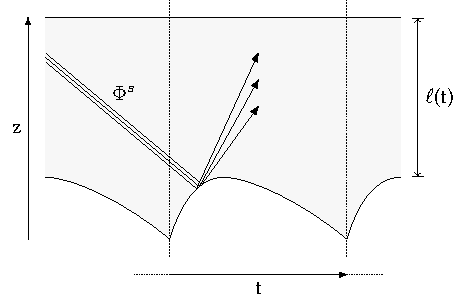
\includegraphics{dispersingFUM.pdf}
\caption{Dynamics of a dispersing Fermi--Ulam Model}\label{f_dispersing}
\end{figure} 

The core observation made in this paper is that the dynamics of dispersing Fermi--Ulam Models sports remarkable geometrical similarities with the dynamics of planar dispersing billiards\footnote{This is one reason why we call such models dispersing. The other explanation in terms of geometric optics is given in \S\ref{SSPSlopes}.}, although with an unusual reflection law. Moreover, our phase space $\csp$ is non-compact, and the smooth invariant measure for $\cm$ is only $\sigma$-finite. Ergodicity of systems with singularities, preserving a smooth infinite measure is discussed for example in~\cite{LenciI, LenciII, Simanyi}. However, our system is significantly more complicated as we explain below.


Recall first, that the study of ergodicity of uniformly hyperbolic systems goes back to Hopf (see~\cite{Hopf}), who analyzed the case where the stable and unstable foliations are smooth. The Hopf argument was extended to smooth uniformly hyperbolic systems\footnote{In such systems stable and unstable foliations are only H\"older continuous, see~\cite{Anosov}.} by Anosov and Anosov--Sinai~\cite{Anosov, AS}. Hyperbolic systems with singularities are discussed in~\cite{SC, KatStr, LW,Pesin,Sinai}. In order to use the Hopf method (which is recalled in \S\ref{ScErg}) one needs to ensure that most points have long stable and unstable manifolds. A classical way to guarantee this fact is to require that a small neighborhood of the singularity set has small measure. In our case the system is non-compact, and an arbitrarily small neighborhood of the singularity set has infinite measure, so a different method has to be employed. A more modern approach relies on the so called Growth Lemma, developed in~\cite{BSC}, see~\cite{ChM} for a detailed exposition. The Growth Lemma implies that each unstable curve intersects many long stable manifolds and vice versa. The Growth Lemma provides a significant improvement on the classical estimate on the sizes of unstable manifolds and it has numerous applications to the study of statistical properties, including mixing in finite and infinite measure settings~\cite{C2, C3, ChZ, DN-Mech}, limit theorems~\cite{C4, DSV}, and averaging~\cite{CD1, CD2, DN-Tube}. However, in order to prove the Growth Lemma one needs to study the structure of the singularity set in great detail. It turns out that the structure of singularities in dispersing Fermi--Ulam models is quite complicated. Continuing the analogy with billiards, it corresponds to billiards with infinite horizon and corner points. The Growth Lemma for billiards with corners was established only recently (see~\cite{jmogy} for finite and~\cite{BrownNandori} for infinite horizon case). Comparing to the aforementioned class of billiards, an additional difficulty in our model is the lack of hyperbolicity at infinity. Indeed, when the velocity is large, the travel time is short and the expansion deteriorates. To address this issue, an accelerated map was studied in~\cite{fum} (see also~\cite{DF, D-icmp} for related results). The main contribution of this paper is to combine the analysis of the high energy regime studied in~\cite{fum}, with the analysis of low energies (mostly based on the ideas of~\cite{ChM} and the advances obtained in~\cite{jmogy}) in order to prove a Growth Lemma valid for all energies. The Growth Lemma also allows us to prove absolute continuity of the stable and unstable laminations, which is a crucial ingredient in the proof of ergodicity via the Hopf argument. Absolute continuity is proved in great generality for finite measure hyperbolic systems with singularities in~\cite{KatStr}, but their results cannot be applied to our infinite measure setting, so a different technique has to be employed.


We hope that the methods developed in this paper will be useful for studying other hyperbolic systems preserving infinite measure (such as, for example, the systems from~\cite{LY, Zh}) and that our Growth Lemma will be useful in studying more refined statistical properties of dispersing Fermi--Ulam models.

Since our analysis has many features in common with the study of billiards, we will try, wherever possible, to employ the same notation as in~\cite{ChM}. However, the arguments necessary for our system require significant modifications in many places, which is, ultimately, the reason for the length of this paper.

The structure of the paper is as follows. In \S\ref{s_hyperbolicity} we describe basic properties of dispersing Fermi--Ulam Models, including invariant cones and expansion rates. \S\ref{s_singularities} discusses the structure of the singularities of the Poincaré map. \S\ref{sec:accel-poinc-map} is devoted to the high energy regime. The results of~\cite{fum} are recalled and extended. \S\ref{ScDistortion} studies distortion of the collision map and obtains regularity estimates on the images of unstable curves. The main technical tool (the Growth Lemma) is then proven in \S\ref{sec:expansion-estimate}. This lemma is used in \S\ref{sec:invariant-manifolds} to study the properties of stable and unstable laminations which lead to the proof of Ergodicity via the Hopf argument in \S\ref{ScErg}. Possible directions of further research are discussed in \S\ref{s_conclusions}. Appendix~\ref{AppRegInf} contains the proof that for all but, possibly, countably many values of $\Delta$, the corresponding model is regular at infinity. The main issue is to show that certain polynomials are not identically zero by estimating their values in a perturbative regime.


\subsection*{A remark about our notation for constants} 
We will use the symbol $\Const$ to denote a constant whose value depends only on $\ell$ (which we assume to be fixed once and for all). The actual value of $\Const$ can change from one occurrence to the next even on the same line.

\section{Hyperbolicity}\label{s_hyperbolicity}
In this section we prove existence of invariant stable and unstable cones for the dynamics and estimate the expansion of tangent vectors. We begin with an essential property of Hamiltonian dynamics.

\subsection{Involution}\label{SSInvolution}
Since Fermi--Ulam Models are mechanical systems, there exists a time-{}reversing involution. Since our system is non-autonomous, we also need to change the time-dependence of the Hamiltonian function, i.e. we need to reverse the motion of the moving wall. For any $\ell$, let $\rell(\ct)=\ell(1-\ct)$ denote the reversed motion, $\bar\exph$ the corresponding extended phase space and $\rflow{s}:\bar\exph\to\bar\exph$ the flow map corresponding to the reversed motion of the wall. Define $\invo:\bR^3\to\bR^3$ so that $\invo:(t,z,v)\mapsto(-t,z,-v)$. Clearly, $\invo(\exph)=\bar\exph$; moreover $\invo$ is an involution (i.e. $\invo\circ\invo = \Id$) which anticommutes with the flow, i.e.
\begin{align*}
\invo\circ\flow{-s} = \rflow{s}\circ\invo.
\end{align*}
Notice a trivial but important fact, that $\ell''\geq\cK$ if and only if ${\bar\ell}''\geq\cK$.

\subsection{Jacobi coordinates} 

In billiards, in order to study the hyperbolic properties of the system, it is convenient to change coordinates in $\exph$ to so-called
\emph{Jacobi coordinates} (see e.g.~\cite{Wojt}). In our case this step is not necessary, since, the coordinates $(z,v)$ turn out to be the Jacobi coordinates of our system. To fix ideas, let us write the action of the flow on the extended phase space $\exph$ as \(\flow{s}:(t,z,v)\mapsto(t+s,z_s,v_s).\) If no collision occurs between $t$ and $t+s$, then we have
\begin{align}\label{e_freeFlight}
z_s&=z+s\cdot v& v_s&=v;
\end{align}
differentiating the above yields $\deh z_s = \deh z + s\deh v$ and $\deh v_s = \deh v$, that is,
\begin{align*}
D_{(t,z,v)}\flow{s}&=\matrixtt{1}{s}{0}{1}=:U_s.
\end{align*}
Assume now that between $t$ and $t+s$ there is exactly one collision which occurs with the moving wall (the case of a collision with the fixed wall is simpler and will be considered in due time as a special case). Let $\bar t$ be the time of the collision, $\bar z=-\ell(\bar t \mod 1)$ be the position of the point mass at the time of the collision, $\prv$ be the pre-collisional velocity (which equals $v$) and $\pov$ the post-collisional velocity (which equals $v_{s}$); then (see Figure~\ref{f_collision}), let
\begin{align}\label{eq:prs=bar-t-tpos=s}
\prs&=\bar t-t&\pos&=s-\prs=t+s-\bar t.
\end{align}


\begin{figure}[!htbp]
\newcommand*\svgwidth{7cm}
%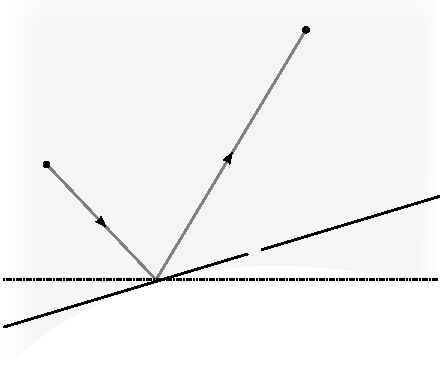
\includegraphics[scale=1]{collision.pdf} 
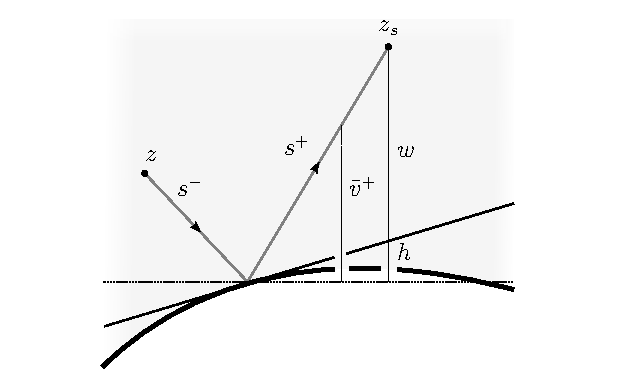
\includegraphics[width=300bp]{collision-complete.pdf}
\caption{Sketch of a collision with the moving wall.}\label{f_collision}
\end{figure}

Let $\slope(\ct)=-\ell'(\ct)$ denote the velocity of the moving wall at time $\ct$ (i.e. the slope of the boundary at the point of collision) and recall that we denote by $w$ the
\emph{post-collisional relative} velocity (i.e. $w = \pov-h$). Recall also that the \emph{Reflection Law} states that, upon a collision of the particle with the wall, the relative post-collisional velocity of the particle becomes the negative of its relative pre-collisional velocity:
\begin{align}\label{WH}
w=\pov-h = -(\prv -h),
\end{align}
which yields $v = \prv = \slope - w$. In summary, we have
\begin{subequations}\label{eq:Jacobi-to-collision-0}
\begin{align}
z &= \bar z - \prs\prv& z_s &= \bar z + \pos\pov\\
v &= \prv = \slope - w & v_s &= \pov = \slope + w.
\end{align}
\end{subequations}
Moreover, let $\curv(\ct)=\ell''(\ct)\geq\cK$ be the opposite\footnote{ This choice of signs reflects the analogous choice which is usually made in the billiard literature.} of the acceleration of the wall at time $\ct$; then:
\begin{align*}
\deh\bar t &= \deh\ct &
\deh\bar z &= \slope \deh\ct &
\deh\slope &= -\curv \deh\ct.
\end{align*}
We thus obtain, computing the differential of~\eqref{eq:prs=bar-t-tpos=s}:
\begin{align*}
d\prs &= dr& d\pos &= -dr.
\end{align*}
Taking the differential of~\eqref{eq:Jacobi-to-collision-0}, and using the above relations, we get
\begin{subequations}\label{e_jacobiToCollision}
\begin{align}
\deh z &=(\slope-\prv)\deh\ct - \prs\deh \prv&
\deh z_s&=(\slope-\pov)\deh\ct + \pos\deh \pov\\
\deh v&=-\curv\deh\ct - \deh w &
\deh v_s&=-\curv\deh\ct + \deh w.
\end{align}
\end{subequations}
We want to study what happens exactly during a collision, therefore we let $\prs,\pos\to 0^+$ and eliminate $\deh\ct$ and $\deh w$ using~\eqref{WH}. We obtain
\begin{align*}
\deh \poz &= -\deh \prz & \deh \pov &= -\cpar\deh \prz- \deh \prv.
\end{align*}
Here $\DS \deh \prz = \lim_{\prs\to0^+}\deh z$ and $\DS \deh \poz = \lim_{\pos\to0^+}\deh z_s,$ and we defined the
\emph{collision parameter} $\cpar=2\curv/w>0$ following the usual notation and terminology of billiards. From the above expression it is clear that some special care is needed to deal with collisions with small $w$. If $w=0$ we say that we have a \emph{grazing} collision.

\begin{rema}\label{rem:grazing_collisions}
Let us examine in more detail the (problematic) case of grazing collisions. Looking at Figure~\ref{f_collision} we observe that the case $w = 0$ corresponds to a situation in which the trajectory (in the $(t,z)$-plane) is tangent to $\ell(t)$. On the one hand, the trajectory is not affected by the fact that the moving wall is present; on the other hand, it is customary to still treat such trajectories as \emph{colliding} with the moving wall, since there exist arbitrarily close trajectories which will undergo a collision. It is important to notice that, the assumption $\curv > 0$ implies that the motion of the wall is (locally) strictly convex; in particular any tangency between the trajectory and the motion of the wall is non-degenerate. In other words, for any grazing collision there exists $\delta > 0$ so that no collision with the moving wall will take place within a time $\delta$.
\end{rema}

Grazing collisions give rise to singularities, as will be explained in detail later. Notice that collisions with the fixed wall yield the same formula with $\cpar=0$.

Define now:
\begin{align*}
L_\cpar&:=\matrixtt{1}{0}{\cpar}{1}.
\end{align*}
Let $\fft:\exph\to\bR_{ > 0}\cup\{\infty\}$ be the time before the next collision with the \emph{moving} wall, including grazing collisions. Clearly, $\fft(t,z,v) = \infty$ if and only if $v = 0$ and $-\min \ell< z \le 0$. $\fft$ is well defined and positive for all other elements of $\exph$. Indeed, since $\ell''(t) > 0$ for any $t$, the intersection of any line with the graph of $-\ell(t)$ is necessarily discrete (see Remark~\ref{rem:grazing_collisions}). We now assume that $(t,z,v)$ is so that $\fft(t,z,v) < \infty$. Let us denote by $\flow{\fft^{+}}$ the flow up to the instant immediately after the collision.\footnote{Recall that, in general, the flow is discontinuous at collisions, see Footnote~\ref{fn:discontinuous-flow}.}
We can write the differential $D_{(t,z,v)}\flow{\fft^{+}}$ as the product
\begin{equation}\label{e_Differential}
{D_{(t,z,v)}\flow{\fft^{+}}}= {(-1)}^{n_\fixw+1} L_{\cpar}U_{\fft}
\end{equation}
where $n_{\fixw}\in\{0,1\}$ is the number of collisions with the fixed wall occurring between time $t$ and $t+\fft$.

\begin{rema}
Since we will employ several coordinates for vectors in $\bR^{2}$, we find convenient to denote, the components of a vector in coordinates $(v,z)$ (resp. $(\ct,w)$) by $(\delta v,\delta z)$ (resp. $(\delta\ct,\delta w)$). The symbol $d$ will denote the differential of a real-valued function, whereas the symbol $D$ will be used to indicate the differential of a map.
\end{rema}

\subsection{Invariant cones}\label{s_invariantCones}

(See~\cite[\S3.8]{ChM}). Since we are dealing with matrices acting on $\bR^2$, it is convenient to deal with slopes, rather than vectors. Slopes of vectors $(\delta v,\delta z)$ in Jacobi coordinates will be denoted by $\pslope= \delta z/\delta v$ and will be called \emph{p-slopes}. A (non-degenerate) matrix acts on slopes as a (non-degenerate) M\"obius transformation. In particular, let $J:\reals\setminus\{0\}\to\reals\setminus\{0\}$ denote the inversion $x\mapsto x\inv$ and for $\alpha\in\bR$ let $T_\alpha$ denote the translation $x\mapsto x+\alpha$. Then the matrix $U_\fft$ induces the map $J\circ T_\fft\circ J$ on slopes, and $L_\cpar$ the map $T_\cpar$, that is:
\begin{align}\label{e_slopeEvolution}
U_\fft & :\pslope\mapsto{\left(\pslope\inv+\fft\right)}\inv & L_\cpar & :\pslope\mapsto\pslope + \cpar
\end{align}
so we can rewrite~\eqref{e_Differential} for p-slopes\footnote{Notice that the factor $ {(-1)}^{n_\fixw+1}$ disappears for slopes.} as follows:
\begin{align}\label{e_evolutionB}
\pslope\mapsto \left[T_{\cpar}\circ J\circ T_{\fft}\circ J\right]\,\pslope.
\end{align}
The above formula immediately shows that the increasing cone $\{\pslope>0\}$ is forward-invariant.\footnote{In fact $J$ clearly preserves such cone; moreover $\fft>0$ by definition and $\cpar>0$ by our hypotheses, which implies that also $T_\fft$ and $T_\cpar$ preserve the increasing cone.}
By the properties of the involution, it is also clear that the decreasing cone $\{\pslope<0\}$ is backward-invariant (i.e. invariant for the time-reversed flow). It is not difficult to express the invariant cones in collision coordinates. Namely, let $\cslope$ denote the slope of a vector $(\delta\ct,\delta w)$ in collision coordinates, that is $\cslope = \delta w/\delta\ct$. Then, using equations~\eqref{e_jacobiToCollision}, we obtain
\begin{equation}\label{e_slopeCollision}
\cslope = - \curv - \prpslope w = \curv - \popslope w,
\end{equation}
where $\prpslope$ and $\popslope$ denote respectively the pre-collisional and post-collisional p-slopes. Thus, the cone $\{\cslope \leq -\cK\}$ (induced by $\prpslope\geq 0)$ is forward-invariant and, correspondingly, $\{\cslope\geq\cK\}$ (induced by $\popslope\leq0$) is backward-invariant.

\begin{defi}\label{def:invariant-cones}
Let the \emph{unstable} and \emph{stable cone field} be, respectively:
\begin{align*}
\coneu_x&=\left\{(\delta\ct,\delta w)\in\tang_x\csp\st -\infty < \delta w/\delta\ct \leq -\cK\right\}\\
\cones_x&=\left\{(\delta\ct,\delta w)\in\tang_x\csp\st \cK\leq\delta w/\delta\ct < \infty\right\}.
\end{align*}
A curve is said to be an \emph{unstable curve}, or u-curve (resp.\ a
\emph{stable curve} or s-curve) if the tangent vector at each point is contained in $\coneu$ (resp. $\cones$). A curve (either stable or unstable) curve is said to be \emph{forward oriented} if the tangent vector at each point has a positive $\ct$-component.
\end{defi}

\begin{rema}
Observe that, in our system, unstable curves are decreasing and stable curves are increasing. This -unfortunately- is the opposite of the situation that arises in \emph{dispersing} billiards.
\end{rema}

Conventionally, we consider curves to be the embeddings as open intervals, i.e. without endpoints. Our previous argument indeed shows that
\begin{align*}
D_{x}\cm{\cconeu_x}&\subset\oconeu_{\cm x}& D_{x}\cm\inv{\ccones_x}&\subset\ocones_{\cm\inv x},
\end{align*}
where $\cconeu$ denotes the closure of $\coneu$ and $\oconeu$ the interior of $\coneu$ (similarly for $\ccones$ and $\ocones$). Moreover by~\eqref{e_Differential} we gather that a forward-oriented unstable (resp. stable) curve is sent by $\cm$ (resp. $\cm\inv$) to a forward-oriented unstable (resp. stable) curve, if the ball has a collision with the fixed wall between the two collisions with the moving wall and to a backward-oriented unstable (resp. stable) curve otherwise.

Further, define the two (closed) cones\footnote{ In the following definitions, we allow vertical vectors with $\delta w/\delta r = \pm\infty$.}
\begin{subequations}\label{e_definitionClosedCones-both}
\begin{align}
\conep_x&= \left\{(\delta\ct,\delta w)\in\tang_x\csp\st 0 \leq \delta w/\delta\ct \leq \infty\right\}\label{e_definitionClosedCones}\\
\conen_x&= \left\{(\delta\ct,\delta w)\in\tang_x\csp\st -\infty \leq \delta w/\delta\ct \leq 0\right\}.\label{e_definitionClosedConesB}
\end{align}
\end{subequations}
Observe that by~\eqref{e_slopeCollision} we have
\begin{equation}\label{PCSlopes}
\popslope=\frac{\curv-\cslope}{w}, \quad\quad
\prpslope=\frac{-\curv-\cslope}{w}.
\end{equation}
From the above equations it follows easily that
\begin{align}\label{e_decreasingCone}
D_{x}\cm\/\conen_x&\subset \coneu_{\cm x}& D_{x}\cm\inv\/\conep_x&\subset \cones_{\cm\inv x}.
\end{align}
Since $\coneu_{x}\subset \conen_x$, $\cones_x\subset\conep_x,$ it follows that in $(\ct,w$)-coordinates we also have that the decreasing cone field $\conen_x$ is forward invariant and the increasing cone field $\conep_x$ is backward invariant.


\subsection{Geometrical interpretation of p-slopes} \label{SSPSlopes}

We recall the following interpretation of tangent vectors (see
e.g.~\cite[\S3.7]{ChM}): vectors in the tangent space correspond to infinitesimal wave fronts. Such wave fronts can be \emph{dispersing, flat} or \emph{focusing}, and these properties are reflected in the sign of the slope $\pslope$.
\begin{itemize}
\item dispersing wave front: nearby trajectories tend to get separated when flowing in positive time; such fronts correspond to vectors, with $\pslope>0$ in Jacobi coordinates.
\item focusing wave front: trajectories which would separate when flowing in negative time, i.e. to trajectories which are focusing in positive time; such fronts correspond to vectors with $\pslope < 0$ in Jacobi coordinates.
\item flat fronts: nearby trajectories will stay at the same distance when flowing in both positive and negative time: such fronts correspond to vectors with $\pslope = 0$.
\end{itemize}
The case $\pslope=\infty$ corresponds to a completely focused front (i.e. all trajectories are emitted from the same point).

\subsection{Expansion}\label{s_Jacobian}
Jacobi coordinates are convenient coordinates on the tangent space to the collision space $\csp$. By~\eqref{e_jacobiToCollision} it follows that
\begin{align*}
\vectt{\delta z}{\delta v}=\matrixtt{w}{0}{\curv}{-1}\vectt{\delta\ct}{\delta w}, \;\;
\vectt{\delta\ct}{\delta w}=\matrixtt{w\inv}{0}{\curv w\inv}{-1}\vectt{\delta z}{\delta v}.
\end{align*}

For any $x\in\csp$, let $\fft(x)\ge 0$ denote the time until the following (possibly grazing) collision with the moving wall. Consider a vector $(\delta z,\delta v)$ of p-slope $\pslope^{+} = \pslope$ at $x$. Then~\eqref{e_freeFlight} implies that, after a flight of duration $\fft$, $(\delta z,\delta v)\mapsto(\delta z_{\fft},\delta v_{\fft})$ where $\delta z_\fft=(1+\fft\pslope)\delta z$ and $\delta v_\fft = \delta v$. On the other hand, at a collision, we have $|\delta \poz|=|\delta\prz|$.

For non-vertical tangent vectors $u = (\delta z,\delta v)$ we define the metric $|u| = |\delta z|$ (the so-called $p$-metric). We then obtain that the expansion of a vector $u$ of p-slope $\pslope$ by the collision map in the p-metric is given by
\begin{equation}\label{ExpPMetric}
\frac{| D_{x}\Phi^{\fft} u|}{|u|} =
\frac{|\delta z_{\fft(x)}|}{|\delta z|}=1+\fft(x)\pslope.
\end{equation}
If $u\in\coneu_{x}$ (i.e. $\pslope>\cpar$), since $\cpar$ is bounded below by $2\cK/w$ we obtain the lower bound
\begin{equation}\label{e_expansionLowerBound}
\frac{|D_{x}\cm u|}{|u|}\geq 1+\frac{2\cK}{w}\fft(x).
\end{equation}

\begin{rema}\label{r_needForAlpha}
Observe that~\eqref{e_expansionLowerBound} does not ensure any uniformity for the expansion of unstable vectors in the $p$-metric. In fact for large relative velocities $\fft\sim w\inv$. Additionally, $\fft$ can be arbitrarily small also for small relative velocities, because of the possibility of rapid subsequent collisions with the moving wall.

We will see later that both these inconveniences can be circumvented by defining an adapted metric and inducing on a suitable subset of the collision space (see Proposition~\ref{p_propertiesAdm}). However, before doing so, it is necessary to study the singularities of our system.
\end{rema}

\section{Singularities}\label{s_singularities}

The existence of invariant cones places Fermi--Ulam Models into the class of \emph{hyperbolic systems with singularities}. This class also contains piecewise expanding maps, dispersing billiards, and bouncing ball systems (see~\cite{ChM, LW, T2, W-particles} and references therein). In hyperbolic maps with singularities, there is a fundamental competition between expansion of vectors inside the unstable cone and fracturing caused by singularities. If fragmentation prevails, such maps can indeed have poor ergodic properties (see e.g.~\cite{T1}). Our goal is to show that this does not happen for (most) dispersing Fermi--Ulam Models; this will be accomplished with the proof of the Growth Lemma in \S\ref{sec:growth-lemma}.

In this section, we collect preliminary information about the geometry of singularities\footnote{The reader familiar with dynamics of dispersing billiards will recognize certain distinctive features of the geometry of singularities (see e.g.~\cite[\S2.10]{ChM}).} of the collision map $\cm$.

\begin{rema}
In the following, if $X\subset\csp$, we will use the notation $\intr X$ ({resp.\ $\clo X$, $\partial X$}) to denote the topological interior (resp.\ closure, boundary) of the set $X$
\emph{with respect to the topology on $\reals^2$} (and not with respect to the relative topology on~$\csp$).
\end{rema}

\subsection{Local structure}\label{ss_singularitiesLocalStructure}

Let us recall the definition of the collision map: $\cm(\ct,w) = (\ct',w')$ means that a point mass that leaves the moving wall at time $\ct$ with velocity $w$ relative to the moving wall will have its next collision with the moving wall at time given $(\bmod \; 1)$ by $\ct'$ and will leave the moving wall with relative velocity $w'$. Recall moreover that $\fft:\csp\to\reals_{\ge\,0}$ is the (lower semi-continuous) function which associates to $(\ct,w)$ the time before the next (possibly grazing) collision with the moving wall. If one considers the
\emph{preceding} collision rather than the following one in the above discussion, we obtain the definition of the inverse map $\cm\inv$.

We define the \emph{singularity set} $\sing0$ to be the boundary $\partial\csp$, i.e.:
\begin{align*}
\sing{0} = \partial\csp =\{w = 0\}\cup \{\ct \in \{0,1\}\}.
\end{align*}
$\sing{0}$ is the set of points in the collision space for which the point mass either just underwent a \emph{grazing} collision (when $w = 0$), or it just left the moving wall at an instant in which the motion of the wall is not smooth (when $r\in\{0,1\}$). Let $x = (\ct,w)\in\csp$; observe that $\fft(x)$ is defined for all $x\in\csp$. There are three possibilities: the trajectory leaving the moving wall at time $\ct$ with relative velocity $w$ may have its next collision with the moving wall
\begin{enumerate}\alphenumi
\item \label{i_regular}
with nonzero relative velocity at an instant when the motion of the wall is smooth. In this case $\cm$ is well-defined on $x$ and $\cm(x)\in\intr\csp = \csp\setminus\sing{0}$.
\item \label{i_grazing}
with \emph{zero} relative velocity at an instant when the motion of the wall is smooth (see Remark~\ref{rem:grazing_collisions}). In this case $\cm$ is well-defined, but may\footnote{In fact it will be always be discontinuous, except in the case described by Lemma~\ref{l_continuityAtxc}.} be discontinuous at $x$ (and it turns out that $ \limsup_{x'\to x}|D \cm|= \infty$). We have $
\cm(x)\in\{r\in(0,1),\ w = 0\}\subset\sing0; $ moreover $\fft$ is also discontinuous at $x$.
\item \label{i_corner}
when the motion of the wall is \emph{not smooth}; $\fft$ is continuous at $x$, but $\cm(x)$ is \emph{not} defined (because the post-collisional velocity is undefined).
\end{enumerate}

We can then define
\begin{align*}
\singForward{} =\sing0 \cup \{x\in\csp\st \text{items~\eqref{i_grazing} {or}~\eqref{i_corner} take place}\}.
\end{align*}
The above also applies to the classification of the \emph{previous} collision, which leads to the analogous definition of $\singBackward{}$. Observe that $\cm$ (resp. $\cm\inv$) is well-defined and smooth on $x$ if and only if $x\in\csp\setminus\singForward{}$ (resp. $x\in\csp\setminus\singBackward{}$). We let $\sing1 = \singForward{}$ (resp. $\sing{-1} = \singBackward{}$) and for $n > 0$ we define, by induction:
\begin{align*}
\sing{n+1} & =\sing{n}\cup\cm\inv(\sing{n}\setminus\singBackward{}) &
\sing{-n-1} & =\sing{-n}\cup\cm\left(\sing{-n}\setminus\singForward{}\right).
\end{align*}
Finally, let $\sing{+\infty} = \bigcup_{n\,\ge\,0}\sing n$ and $\sing{-\infty} = \bigcup_{n\,\le\,0}\sing n$. Notice that, for any $k\in\bZ$, the map $\cm^{k}$ is well-defined and smooth on $x$ if and only if $x\in\csp\setminus\sing{k}$.

\begin{lemm}[Local structure of singularities]\label{l_localSing}
For $k > 0$ the set $\sing{k}\setminus\sing{0}$ (resp. $\sing{-k}\setminus\sing0$) is a union of smooth \emph{stable} (resp. \emph{unstable}) curves. In particular $\sing{k}$ (resp. $\sing{-k}$) is a union of smooth curves tangent\footnote{ Here and below we say that a curve is tangent to a cone field if the tangent to the curve belongs to the cone at every point.} to the cone field $\conep$ (resp. $\conen$) defined by~\eqref{e_definitionClosedCones-both}.
\end{lemm}


We will prove the above statement for $\sing{-k}$. The analogues for $\sing{k}$ can be obtained using the involution. Moreover, since the unstable cone is $\cm$-invariant, it suffices to prove the statement for $\sing{-1} = \singBackward{}$.

\begin{enonce}{Sublemma}
Let $x\in\singBackward{}\setminus\sing0$, then the p-slope of $\singBackward{}$ at $x=(\ct,w)$ is given by
\begin{subequations}\label{e_slopeSingularity1}
\begin{align}
\pslope &= \cpar(x)+1/\fft_{-1}(x)>0.\label{e_pslopeSingularity1}
\intertext{ Equivalently, the slope in collision coordinates is given by }
\cslope &= -\curv(\ct) - w/\fft_{-1}(x)\leq -\cK.\label{e_cslopeSingularity1}
\end{align}
\end{subequations}
\end{enonce}
\begin{proof}
Observe that each curve in $\singBackward{}$ is formed by trajectories for which either $\ct_{-1}=0$, or $w_{-1}=0$. In the first case, such trajectories draw a wave front which is emitted from a single point, therefore it is immediate that $\pslope_{-1}^+=\infty$. We claim that also in the second case $\pslope_{-1}^+=\infty$, which then immediately implies equations~\eqref{e_slopeSingularity1} using~\eqref{e_evolutionB}. In fact consider two nearby trajectories which leave the wall with zero relative velocity at times $\ct$ and $\ct'=\ct+\Delta\ct$. Let $v$ and $v'=v+\Delta v$ be the corresponding outgoing velocities. Observe that $\Delta v\sim\curv\Delta \ct$. On the other hand, the second trajectory at time $\ct$ will have height $z'=z+\Delta z$, where $\Delta z\sim\curv{(\Delta\ct)^2}$. We conclude that $ \pslope^+_{-1}=\lim_{\Delta\ct\to0}\Delta v/\Delta z=\infty$.
\end{proof}
\begin{rema}
The corresponding formulae for the slopes of $\singForward{}$ at any $x=(\ct,w)\in\singForward{}\setminus\sing0$ are
\begin{subequations}\label{e_slopeSingularityForward}
\begin{align}
\pslope &= -1/\fft_{0}(x) < 0\\
\cslope &= \curv(\ct) + w/\fft_0(x) > \cK.
\end{align}
\end{subequations}
\end{rema}

\begin{rema}\label{remark:singularity-order}
The proof of Lemma~\ref{l_localSing} actually shows that any curve in $\sing{k}$ (resp. $\sing{-k}$) passing through a point $x$ is tangent to the cone field $\conep\cap D_{\cm^{k}x}\cm^{-k}\conen$ (resp. $\conen\cap D_{\cm^{-k}x}\cm^{k}\conep$).
\end{rema}
\subsection{Global structure.}\label{s_globalSingularities}
We now begin the description of the global structure\footnote{ The structure depends on our simplifying hypotheses on the motion of the wall. If $\ell$ had more than one break point, the set $\sing{1}$ would have a much more complicated structure, although its key features will be similar. Moreover, the structure of $\sing{k}$ for $k>1$ would also be essentially similar in the case we have multiple breakpoints.} of the singularity sets $\singBoth$. Let us first introduce some convenient notation.

Let $\ellu=\max\ell=\ell(0)=\ell(1)$. Since $\ell$ is strictly convex, it has a unique critical point (a minimum), which we denote by $\ctc\in(0,1)$. Set $\elll=\min\ell=\ell(\ctc)$ and $\xc=(\ctc,0)$. Recall that $\slope(\ct)=-\ell'(\ct)$ and define
\begin{align*}
\slopel\!=\!\min\slope\!=\!\lim_{\ct\to1}\slope(\ct)\!<\!0,\; \slopeu\!=\!\max\slope\!=\!\lim_{\ct\to0}\slope(\ct)\!>\!0,
\;
\slopeb=\slopeu-\slopel>0.
\end{align*}
We remark that in this new notation, we can write~\eqref{DefDelta} as
\begin{align*}
\Delta &= -\ellu \slopeb\int_0^1 \ell^{-2}(t) dt.
\end{align*}

Observe that the point $\xc$ is a fixed point for the dynamics: it corresponds to the configuration in which the point mass stays put at distance $\elll$ from the fixed wall, and the moving wall hits it with speed $0$ at times $\ctc+\integers$. Moreover, points arbitrarily close to $\xc$ may have arbitrarily long free flight times i.e.
\begin{align*}
\limsup_{x\to\xc}\fft(x) = \infty.
\end{align*}


Next, we identify a special region of the phase space. It is clear that, if the relative velocity of the point mass at a collision with the moving wall is sufficiently large, then the particle will necessarily have to bounce off the fixed wall before colliding again with the moving wall. On the other hand, if the velocity at a collision with the moving wall is comparable with the velocity of the wall itself, then the particle could have two (or a priori more) consecutive collisions with the moving wall before hitting the fixed wall.\footnote{ In the case of billiards this corresponds to so-called
\emph{corner series}.}
\begin{defi}
A collision with the moving wall is called a \emph{recollision} if it is immediately preceded by another collision with the moving wall; it is called a \emph{simple collision} otherwise. A recollision is said to be \emph{regular} unless it undergoes a grazing collision on either the recollision or on the previous collision or it is a collision with the singular point $\xc$. We denote with $\reco\subset\csp$ the open set of points corresponding to regular recollisions and let $\backReco=\cm\inv\reco$.
\end{defi}

The following lemma provides a description of the sets $\reco$ and $\backReco$.
\begin{lemm}\label{l_forwardReco}
Let $\singReco^- = \cm([\ctc,1]\times\{0\})$ and $\singReco^+ = \cm\inv([0,\ctc]\times\{0\})$. Then:
\begin{enumerate}\aenumi
\item\label{lemm3.7.a1} $\singReco^-$ is a connected u-curve that leaves $(0,\slopeb)$ with slope $-\infty$ and reaches $\xc$ with slope $-\curv({\ctc})$;
\item\label{lemm3.7.a2} $\reco$ is the interior of the curvilinear triangle whose sides are the (horizontal) segment $[0,\ctc]\times\{0\}$, the (vertical) segment $\{0\}\times[0,\slopeb]$ and $\singReco^-$.
\end{enumerate}
\begin{enumerate}\benumi
\item \label{lemm3.7.b1}$\singReco^+$ is a connected s-curve that leaves $\xc$ with slope $\curv(\ctc)$ and reaches $(1,\slopeb)$ with slope $\infty;$
\item \label{lemm3.7.b2}$\backReco$ is the interior of the curvilinear triangle whose sides are the (horizontal) segment $[\ctc,1]\times\{0\}$, the (vertical) segment $\{1\}\times[0,\slopeb]$ and $\singReco^+$.
\end{enumerate}
\end{lemm}
\begin{figure}[!h]
\newcommand*\svgwidth{7.5cm}
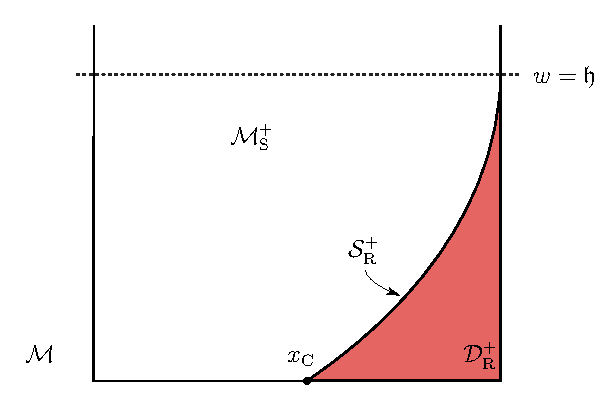
\includegraphics[width=292bp]{recollisionRegion-complete.pdf}
%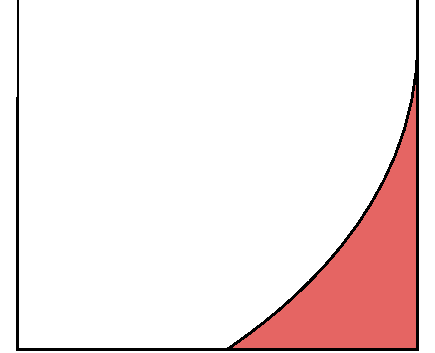
\includegraphics[scale=1]{figures/recollisionRegion.pdf} 
\caption{The recollision region $\backReco$.}\label{f_recollisionRegion}
\end{figure}
\pagebreak
\begin{proof}
We prove part (a). Part (b) follows from part (a) and the properties of the involution. Let $U$ denote the curvilinear triangle in $(t,z)$-space bounded by $\Gamma_1$--the wall trajectory for $t\in [r_C,1]$, $\Gamma_2$--the wall trajectory for $t\in [1, r_C+1]$ and $\Gamma_3$--the horizontal segment joining the highest points of those trajectories. By our convexity assumption on $\ell$ and elementary geometrical considerations, any trajectory $x = (r,0)$ with $r\in[\ctc,1]$ stays inside $U$. Hence its next collision necessarily occurs on the moving wall. This in turn implies that the u-curve $\singReco^- = \cm([\ctc,1]\times \{0\})$ is connected (since it cannot be cut by singularities). It is then trivial to check that $\cm(1,0)=(0,\slopeb)$, which implies that $\singReco^-$ connects $(0,\slopeb)$ with the fixed point $\xc$. Our statements about the tangent slope at $(0,\slopeb)$ and $\xc$ immediately follow from~\eqref{e_cslopeSingularity1} observing that
\begin{align*}
\lim_{\ct\to 1}\fft((\ct,0)) &= 0&
\lim_{\ct\to\ctc^+}\fft((\ct,0)) &= 1.
\end{align*}

It remains to prove~\eqref{lemm3.7.a2}. First, consider a collision that occurs at a point $(\ct,w)$ with $\ct \in (\ctc,1]$. The incoming trajectory lies above the tangent to $\ell$ at $\ct$, which, in turn, lies above the graph of $\ell$ (for $\ct' < \ct$) by convexity of $\ell$. In particular it is above the graph of $\ell$ at time $\ctc$, that is, it gets above the maximal height of the wall and its velocity at time $\ctc$ is negative. Hence, necessarily, the preceding collision will occur with the fixed wall, proving that $\reco\subset[0,\ctc]\times\reals^+$. It remains to check that any point in $[0,\ctc]\times\reals^+$ lying below $\singReco^-$ corresponds to a recollision, whereas any point lying above $\singReco^-$ corresponds to a single collision. So pick $r\in [0, \ctc]$. By~\eqref{lemm3.7.a1} there is $\ct^*\in [\ctc, 1]$ such that $\cF(\ct^*,0)=(r, w^*)\in \singReco^-$. Let $\Gamma$ be the trajectory (in $(t,z)$-space) from $(\ct^*,0)$ to $(r, w^*)$ and $V\subset U$ be the region bounded by (a part of) $\Gamma_1,$ a part of $\Gamma_2,$ and $\Gamma$. There are two cases.
\begin{enumerate}\romanenumi
\item $w\leq w^*$. Then the backward trajectory of $(r, w)$ is contained in $V$ and so it crosses $\Gamma_1$ before colliding with the fixed wall.
\item $w\geq w^*$. Then the backward trajectory of $(r, w)$ is above $\Gamma$ so if it crossed $\Gamma_1$ this would happen at some time $\ct'<\ct^*$. However by convexity, any orbit starting at time $\ct'$ lies strictly above $\Gamma$ so it can not hit the moving wall at time $r$.
\end{enumerate}
This concludes the proof.
\end{proof}

\begin{rema}\label{r_thereCanBeOnlyOne}
The above lemma implies that $\clo\backReco\cap\clo\reco=\{\xc\}$, i.e. the number of consecutive collisions with the moving wall is at most $2$ (except for the singular point $\xc$, which is a fixed point of the dynamics).
\end{rema}

\begin{rema}\label{r_boundFreeFlight}
Let $x_0=(r_0,w_0)$; if $x_0\not\in\clo\backReco$, then $\fft(x_0)$ satisfies the bound:
\begin{align}\label{e_boundFreeFlight}
\frac{2\elll}{w_1-\slope(\ct_1)} = \frac{2\elll}{w_0+\slope(\ct_0)} \leq \fft(x_0) \leq
\frac{2\ellu}{w_0+\slope(\ct_0)} = \frac{2\ellu}{w_1-\slope(\ct_1)}.
\end{align}
\eqref{e_boundFreeFlight} follows since $w_0+h(r_0)=w_1-h(r_1)$ is the speed of the particle between the collision at $\ct_{0}$ and the next collision with the moving wall, and $\elll\le\ell(\ct) < \ellu$. Observe moreover that $w_0+h(r_0)>0$, otherwise the next collision would certainly be a recollision, since the absolute velocity would be non-positive. On the other hand, if $x\in\backReco$, $\fft(x)$ may be arbitrarily small.
\end{rema}

We record in the following lemma an observation which will be useful on several occasions.
\begin{lemm}\label{lem:geometry}
If $x = (\ct,w)$ is so that either $\fft(x) \geq 2$ or $\fft_{-1}(x)\geq 2$ then:
\begin{align*}
x \in \left\{w < \Const \tau^{-1/2},\; |\ct-\ctc|< \Const
\tau^{-1/2} \right\}.
\end{align*}
\end{lemm}
\begin{proof}
It suffices to prove the result under the assumption $\tau(x)\geq 2$, since the other case follows by applying the involution. Since $\tau(x)\ge 2$, in particular $x\nin\cl\backReco$; we thus apply~\eqref{e_boundFreeFlight} and conclude that
\begin{equation}\label{AVDNu}
0<w+h(\ct) \le 2\ellu/\tau.
\end{equation}
We also have $\ell(\ct)-\elll = \cO(1/\tau)$, because otherwise $(\ct, w)$ would be in the recollision region. Since the critical point $\ell$ at $\ctc$ is quadratic (because $\curv(\ctc) > 0$), it follows that $|\ct-\ctc|\leq \frac{\bar C}{\sqrt{\tau}}$ giving the second inclusion. It follows that $|h(\ct)|\leq \frac{\hat C}{\sqrt{\tau}}$. Now the first inclusion follows from~\eqref{AVDNu}.
\end{proof}

Define $\csps^- = \clo(\csp\setminus\clo\reco)$ and $\csps^+ = \clo(\csp\setminus\clo\backReco)$. The curve $\singReco^-$ (resp. $\singReco^+$) is one among the unstable (resp. stable) disjoint curves whose union form the set $\singBackward{}$ (resp. $\singForward{}$). The other curves will cut $\csps^-$ (resp. $\csps^+$) in countably many connected components, as we now describe\footnote{The structure of singularities for dispersing Fermi--Ulam Models is remarkably similar to the one described in~\cite[\S4.10]{ChM} for the singularity portrait in a neighborhood of a singular point of a billiard with infinite horizon. We refer to the discussion presented there for further insights; here we provide a qualitative description which however suffices for our purposes.}. Let us first introduce some convenient notation: we define the \emph{left boundary} $\lboundary\csps^\pm = \{(\ct,w)\in\partial\csps^\pm \st
\ct\in[0,\ctc]\}$ and the right boundary $\rboundary\csps^\pm = \{(\ct,w)\in\partial\csps^\pm \st
\ct\in[\ctc,1]\}$.
%\newcommand{\singMap}{\Gamma}
\begin{lemm}\label{LmSingF}
There exist countably many $C^1$-smooth unstable curves $\{\singBackward{\indCell}\}_{\indCell = 0}^{\infty}$ with the following properties
\begin{enumerate}\alphenumi
\item\label{lemm3.11.1} $\singBackward{\indCell}\cap\singBackward{\indCell'} = \emptyset$ if $\indCell\ne\indCell'$.
\item\label{lemm3.11.2} $\singBackward{} = \singReco^-\cup\bigcup_{\indCell = 0}^{\infty}\singBackward{\indCell}$.
\item\label{lemm3.11.3} $\singBackward{0}$ is unbounded: its left endpoint approaches $(0,\infty)$ and the other endpoint is in $\rboundary\csps^-$.
\item \label{lemm3.11.4}$\singBackward{\indCell}$ for $\indCell > 0$ is compact and joins $\lboundary\csps^-$ to $\rboundary\csps^-$.
\item\label{lemm3.11.5} $\singBackward{\indCell}$ approaches $\xc$ for $\indCell\to\infty$; more precisely:
\begin{align*}
\singBackward{\indCell}\subset\left\{w < \Const \indCell^{-1/2},\; |\ct-\ctc|< \Const \indCell^{-1/2} \right\}.
\end{align*}
\item\label{lemm3.11.6} There exists $c > 0$ such that $\singBackward{\indCell}$ is tangent to the cone
\begin{align*}
\hat{\coneu_{\indCell}} := \left\{-\curv(\ct)-c\indCell^{-3/2}\le\delta w/\delta r\le -\curv(\ct)\right\}.
\end{align*}
\end{enumerate}
The corresponding statements hold for $\singForward{}$ using the involution.
\end{lemm}
\begin{proof}
A point $x'$ can be in $\singBackward{}$ for two different reasons: its previous collision with the moving wall $x = (\ct,w)$ may have occurred either at an integer time (item~\eqref{i_corner} in the definition of $\sing0$) or at a non-integer time with a grazing collision (item~\eqref{i_grazing} in the definition of $\sing0$). If $x'$ is a recollision, then $x'\in\singReco^-$ (and hence $\ct\in[\ctc,1]$ and $w = 0$), otherwise we can choose $x\in\lboundary\csps^+$.

For any $\indCell\in\integers_{\ge\,0}$ define $
\sing0_\indCell = \{x\in\lboundary\csps^+\st\fft(x)\in[\indCell,\indCell+1]\}. $ Notice that $\cm$ is smooth in the interior of these curves\footnote{ Smoothness is obvious unless $(0,0)\in\intr\sing0_\indCell$; even in this case it holds true, and follows from arguments described in~\cite[after Exercise~4.46]{ChM}}. Observe that $\partial^{l}\csps^{+}$ comprises only horizontal {or} vertical segments, whose tangent vectors belong to $\conen_{x}$ (recall~\eqref{e_definitionClosedConesB}); we thus conclude, using~\eqref{e_decreasingCone} that $\cm(\intr\sing0_\indCell)$ is a $C^1$-smooth unstable curve. Define
\begin{align*}
\singBackward{\indCell} = \cl\cm(\intr\sing0_\indCell).
\end{align*}
Items~\eqref{lemm3.11.1} and~\eqref{lemm3.11.2} then follow by construction.

Next, it is easy to see that if $w$ is sufficiently large, then the trajectory will bounce off the fixed wall and collide with the moving wall after a short time $\fft\in(0,1)$; in particular $\sing0_0$ is unbounded while $\sing0_\nu$ and $\singBackward\nu$ are bounded for $\nu>0$.

Next, as $w$ increases to $\infty$, the point $\cm (0,w)=(\ct', w')$ where $\ct'$ is small and $w'$ is large. On the other hand when $x\in\sing0_0$ approaches the (only) boundary point of $\sing0_0$, the point $\cm x$ will necessarily tend to $\rboundary\csps^-$. This proves item~\eqref{lemm3.11.3}. Item~\eqref{lemm3.11.4} follows from analogous arguments.

Item~\eqref{lemm3.11.5} follows by applying Lemma~\ref{lem:geometry} to an arbitrary point in $\singBackward{\indCell}$. Finally, item~\eqref{lemm3.11.6} follows from~\eqref{e_cslopeSingularity1} and item~\eqref{lemm3.11.5}.
\end{proof}

\begin{lemm}[Continuation property]
For each $n\ne 0$, every curve $S\subset\sing n\setminus \sing0$ is a part of some monotonic continuous (and piecewise smooth) curve $\sing{*}\subset\sing n\setminus \sing 0$ which terminates on $\sing0 = \partial\csp$ (note that $\sing{*}$ might be unbounded).
\end{lemm}

\begin{proof}
It suffices to prove the property for $n > 0$, since the case $n < 0$ follows by involution. The statement holds for $n = 1$ by Lemma~\ref{LmSingF}. {We now proceed by induction. Suppose the result holds for some $n>0$ and} $S\subset\sing {n+1}\setminus\sing n$. {Then, by construction}, $S$ terminates on either $\sing0$ or $\sing n$. However if it terminates on $\sing n$, then by inductive hypothesis it can be continued as a piecewise smooth curve to $\sing 0$.
\end{proof}

The curves $\{\singBoth_{\indCell}\}_{\indCell\,\ge\,0}$ cut $\csps^\pm$ in countably many connected components which we denote by $\{\cell^+_\indCell\}$ (resp. $\{\cell^-_\indCell\}$) and we call
\emph{positive} (resp. \emph{negative}) \emph{cells}. Indexing is defined as follows: for $\indCell > 0$ we let $\cell^\pm_\indCell$ denote the component whose boundary contains $\singBoth_{\indCell-1}$ and $\singBoth_{\indCell}$ and let $\cell^\pm_0$ denote the remaining cell. The cells $\cell^+_\indCell$ admit also an intrinsic definition as
\begin{align}\label{e_defCell}
\cell^+_\indCell &= \intr\left\{x\in\csps^+ \st \ct(x)+\fft_0(x)\in(\indCell,\indCell+1)\right\};
\end{align}
observe that each positive cell is indexed by the number of lines $\ct \in \bZ$ which are crossed by the trajectory between the current and the next collision in the extended phase space $\exph$. A similar intrinsic characterization can be given for the negative cells $\cell^-$. We summarize in the following lemma some properties of positive cells that follow from the above discussion.

\begin{lemm}[Properties of positive cells]\label{l_singularityStructure}
\leavevmode
\begin{enumerate}\alphenumi
\item \label{i_disjointCells}
The cells $\{\cell^+_\indCell\}_{\indCell\,\ge\,0}$ are open, connected and pairwise disjoint.
\item \label{i_partitionCells}
We have $\DS
\intr\csps^+\setminus\singForward{}=\bigcup_{\indCell=0}^\infty\cell^+_\indCell. $
\item \label{i_adjacentCells}
$\clo\cell^+_\indCell\cap\clo \cell^+_{\indCell'} = \emptyset$ if $|\indCell-\indCell'| > 1$; moreover if $\bar x\in\clo\cell^{+}_{\indCell}\cap\clo\cell^{+}_{\indCell+1}$, we have either
\begin{align*}
\lim_{\cell^{+}_{\indCell}\,\ni\,x\to\bar x}\cm x&\in\{1\}\times\reals^+,&
\lim_{\cell^{+}_{\indCell+1}\,\ni\,x\to\bar x}\cm x&\in\{0\}\times\reals^+,
\\
\intertext{or}
\lim_{\cell^{+}_{\indCell}\,\ni\,x\to\bar x}\cm x&\in[0,1]\times\{0\},&
\lim_{\cell^{+}_{\indCell+1}\,\ni\,x\to\bar x}\cm x&\in\singReco^{-}.
\end{align*}
\item for any $\bar\indCell$ there exists $\eps$ so that the ball of radius $\eps$ centered at $\xc$ does not intersect $\bigcup_{\indCell = 0}^{\bar\indCell} \cell^+_\indCell$.
\item \label{i_boundedCells}
for $\indCell > 1$, we have $\cell^{+}_{\indCell}\subset\{w < \Const \indCell^{-1/2},\; |\ct-\ctc|< \Const \indCell^{-1/2} \}$.
\end{enumerate}
\end{lemm}

\begin{rema}\label{r_singularityStructureBackwards}
Using the involution, the above lemma also describes (with due modifications) the negative cells $\cell^-_\indCell = \cm\cell^+_\indCell$.
\end{rema}

Despite the fact that the singular point $\xc$ is accumulated by singularities (both forward and backward in time), we have the following result.
\begin{lemm}\label{l_continuityAtxc}
For every $\eps > 0$ there exists a $\delta > 0$ so that
\begin{align*}
\cm\left(B(\xc,\delta)\setminus\sing1\right)\subset B(\xc,\eps).
\end{align*}
\end{lemm}
\begin{proof}
If $x\in B(\xc,\delta)\setminus\sing1$ there are two possibilities; either $x\in B(\xc,\delta)\cap\backReco$ or $x\in B(\xc,\delta)\cap\cell^+_\indCell$ for some large $\indCell$. In the former case $\cm$ is continuous in $\backReco$ and $\DS \lim_{\backReco\,\ni\,x\to(\ctc,0)}\cm x = \xc$, so we only need to check the latter case. However, if $x\in\cell^+_\indCell$, then, by definition $\cm x\in\cell^-_\indCell$ and we conclude the proof since the cells $\{\cell^-_\indCell\}$ also accumulate to $\xc$ by Lemma~\ref{l_singularityStructure}$\MK$\eqref{i_boundedCells} and Remark~\ref{r_singularityStructureBackwards}.
\end{proof}

In view of Lemma~\ref{LmSingF}, a u-curve $W$ can in principle be cut by singularities of $\cm$ in countably many connected components.\footnote{ This problem is certainly familiar to the reader acquainted with the theory of dispersing billiards with infinite horizon.} The next lemma ensures that this may only happen in a neighborhood of the singular point $\xc$.
\begin{lemm}\label{l_finitelyManySectors}
Let $x\in\csp\setminus\{\xc\}$. For any $l > 0$, the set $\sing{l}$ cuts a sufficiently small neighborhood of $x$ in finitely many connected components.
\end{lemm}
\begin{proof}
Assume that for an arbitrarily small ball $\cU\ni x$ there exists $0 < l'\le l$ so that $\cU\setminus\sing {l'-1}$ has finitely many connected components and $\cU\setminus\sing {l'}$ has infinitely many. We conclude that there exists a connected component $\cU'$ of $\cU\setminus\sing {l'-1}$ which is cut by $\sing {l'}$ in infinitely many connected components. By definition $\cm^{l'-1}$ is smooth on $\cU'$ and, by our assumption, $\cm^{l'-1}\cU'$ intersects infinitely many positive cells $\cell^+$. We gather that there exists a sequence $x_m\in\cU'\cap\cm^{-(l'-1)}\cell^+_{\indCell_m}$, where $\indCell_m\to\infty$; by Lemma~\ref{l_singularityStructure} we have $\cm^{l'-1}x'_m\to\xc$, which by Lemma~\ref{l_continuityAtxc} implies that $x'_n\to\xc$, that is $\xc\in\cl\cU$. Since $\cU$ can be taken to be arbitrarily small, we conclude that $x = \xc$.
\end{proof}

For $l_- \le 0 \le l_+$, define $\sing{l_-,l_+} = \sing{l_-}\cup\sing{l_+}$: then $\csp\setminus\sing{l_-,l_+}$ is given by a (countable) union of connected components. A point $x\in\sing{l_-,l_+}$ is said to be a
\emph{multiple point of $\sing{l_-,l_+}$} if it belongs to the closure of at least three such connected components; we denote the set of multiple points of $\sing{l_-,l_+}$ by $\mult{l_-,l_+}$.


\begin{lemm}\label{l_singularPointNotMultiple}
The singular point $\xc\nin\mult{l_-,l_+}$ for any $l_- \le 0 \le l_+$.
\end{lemm}
\begin{proof}
By Lemma~\ref{l_singularityStructure} the only connected component of $\csp\setminus\sing1$ whose closure meets $\xc$ is $\backReco$. This proves our statement for $l_- = 0,\ l_+ = 1$. Now consider a connected component $\cc$ of $\csp\setminus\sing{0,2}$; by definition there exist $\indCell,\indCell'\in\{\recoPrivate,0,1,\cdots\}$ so that $\cc = \cell^+_\indCell\cap\cm\inv\cell^+_{\indCell'}$. If $\cl\cc\ni\xc$, then by the above discussion $\indCell = \recoPrivate$, which by Remark~\ref{r_thereCanBeOnlyOne} implies that $\indCell'\ne\recoPrivate$. But then we would have $\cl\cm\inv\cell^+_{\indCell'}\ni\xc$, which by Lemma~\ref{l_continuityAtxc} implies that $\cl\cell^+_{\indCell'}\ni\xc$, contradicting Lemma~\ref{l_singularityStructure}. The statement for general $l_-$ and $l_+$ then follows by applying Lemma~\ref{l_continuityAtxc}.
\end{proof}

\section{Accelerated Poincaré map.}\label{sec:accel-poinc-map}
The analysis of \S\ref{s_hyperbolicity} shows that expansion of the collision map $\cm$ is small for large energies: the hyperbolicity of $\cm$ is indeed rather weak in this region. It is thus convenient to consider an induced map, obtained by skipping over collisions that happen in the same fundamental domain for $\ell$. In this section we discuss the resulting accelerated map $\cmp$. In particular, we will recall the results of~\cite{fum}, where the large energy regime for piecewise smooth Fermi--Ulam Models was studied in detail. At the same time, we will also present some new technical estimates which are needed for the proof of our Main Theorem.
\subsection{Number of collisions per period.} Recall the definition of positive and negative $\indCell$-cells given in the previous section (see~\eqref{e_defCell}). Define (see Figure~\ref{f_inducingRegion}):
\begin{align}\label{e_definitionInducedSpace}
\cspi = \clo\left(\csp\setminus \clo\cell^-_0\right).
\end{align}
\begin{figure}[!h]
\def\svgwidth{5cm} 
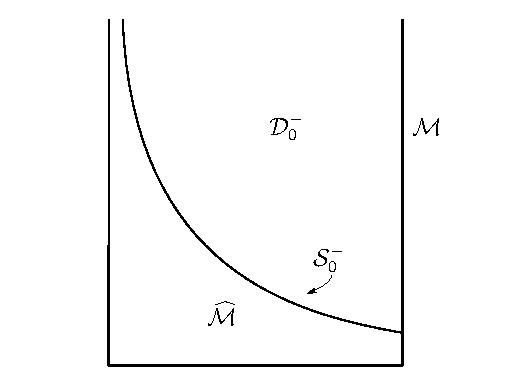
\includegraphics[width=245bp]{inducingSet-complete.pdf}
\caption{The inducing set $\cspi$; note that the geometry can be different depending on the properties of $\ell$. In fact, it is possible for $\singBackward 0$ to terminate at $\{w = 0\}$ rather than at $\{\ct = 1\}$ (see Remark~\ref{rem_terminateS0}).}\label{f_inducingRegion}
\end{figure}

\begin{rema}\label{r_boundary cspi}
Observe that $\partial\cspi$ is the union of vertical curves, horizontal curves and the unstable curve $\singBackward0$. In particular, each curve in $\partial\cspi$ is compatible with the cone field $\conen$ {defined by~\eqref{e_definitionClosedConesB}.}
\end{rema}

\begin{rema}\label{rem_terminateS0}
By construction, $\singBackward 0$ terminates on $\{w = 0\}$ if and only if $\cl \cell^{-}_{0}\ni(1,0)$, which is in turn equivalent to the following geometrical criterion: consider the trajectory that terminates\footnote{Recall that a trajectory that collides with the moving wall at a singularity is undefined after the collision.} at the corner point $\ct' = 1$ tangent to $\ell$ (i.e. with $\prv = -\ell'(0^{-})$). This trajectory emanates from some point $(\ct,w)$; then, by definition, $\cl \cell^{-}_{0}\ni(1,0)$ if and only if $\ct\in[0,1)$. Observe that if $\ct = 0$, then $\singBackward 0$ terminates at $({1,0})$.
\end{rema}
\begin{rema}
Observe that the curve $\singBackward 0$ is asymptotically $1/w$-close to $\{\ct = 0\}$ as $w\to\infty$; in particular $\mu(\cspi\cap\{w < w^{*}\}) \sim w^{*}$, and $\mu(\cspi) = \infty$.
\end{rema}

Let $\cE_0 = \intr\csp$ and, for any $n\in\naturals$, define
\begin{align*}
\cE_{n} &= \left\{x\in \csp\setminus\sing{n-1}\st\cm^{k}x\in\cell_0^+ \text{ for any }0\le k < n\right\}.
\end{align*}
Observe that, by construction, $\cE_n\supset\cE_{n+1}$ and $\cE_n\supset\cm\cE_{n+1}$; since $\cell_0^+\cap\sing1 = \emptyset$, we conclude by induction that $\cE_n\cap\sing{n} = \emptyset$.

For any $n > 0$, define $\cEs_n = \cE_{n-1}\setminus\cE_{n}$. Observe that, if $x\in\cEs_1\setminus\sing{1}$, then $\cm$ is well defined and smooth at $x$, and moreover $\cm x\in\cspi$; more generally, for any $k\ge 1$, if $x\in\cEs_{k}\setminus\sing{k}$, then the map $\cm^k$ is well defined and smooth at $x$, and moreover $\cm^kx\in\cspi$. For any $x\in\intr\csp$, define:
\begin{align*}
\Np(x) = \sum_{k\,\ge\,0} 1_{\cE_k}(x) = \max\{n\ge0\st \cE_n\ni x\} +1.
\end{align*}
If $x\in\cEs_n$, our construction implies that $\Np(x) = n$. Finally, let
\begin{align*}
\singt+ = \sing0\cup \bigcup_{k\,\ge\,0} \left(\sing{k+1}\cap \cE_k\right).
\end{align*}
Observe that, for any $k$ we have $\cEs_{k}\cap\singt+ = \cEs_{k}\cap\sing{k}$ and $\partial\cEs_{k}\subset\singt+$. In particular, for any $k > 0$, the function $x\mapsto\min\{k,\Np(x)\}$ is constant on each connected component of $\csp\setminus\sing{k}$. Moreover, by construction, $\singt+$ is a countable union of $C^1$-smooth stable curves with
\begin{align*}
\singForward{}\subset\singt+\subset\sing{+\infty}.
\end{align*}
By the above considerations, we conclude that if $x\in\csp\setminus\singt+$ and $\Np(x) < \infty$, then $\cm^{\Np(x)}$ is well-defined and smooth at $x$ and $\cm^{\Np(x)}x\in\cspi$. We now proceed to show that $\Np$ is finite for any $x\in\intr\csp$.
\begin{lemm} \label{LmFRet}
The sets $(\cEs_n)_{n > 0}$ form a partition$\pmod0$ of $\csp.$ Moreover for any $x = (r,w)\in\intr\csp$:
\begin{align}\label{e_weakBoundOnNp}
1\le\Np(x)\le \Const (w+1).
\end{align}
\end{lemm}
\begin{proof}
We claim that for sufficiently large $n$:
\begin{align}\label{e_linearBoundOncE}
\cE_n \subset \{w\ge \Const n-\slopeu\}.
\end{align}

Observe that~\eqref{e_linearBoundOncE} implies that
\begin{align*}
\bigcap_{k\,\ge\,0}\cE_k = \emptyset;
\end{align*}
which in particular implies that the sequence $(\cEs_n)_{n\,>\,0}$ forms a partition$\pmod 0$ of $\csp$. The estimate~\eqref{e_weakBoundOnNp} also immediately follows from~\eqref{e_linearBoundOncE}.

We proceed with the proof of our claim. Assume $x\in\cE_n$ and let $x_k =(r_k,w_k) = \cm^k x$. By construction, we have for any $0\le k < n$ that $x_k\in\cell^+_0$, i.e. $\ct_{k}+\fft(x_{k}) \in(0,1)$. By induction, this implies $\ct_n = \ct_{0}+\sum_{k=0}^{n-1}\fft(x_k) < 1$. In particular
$\sum_{k=0}^{n-1}\fft(x_k) < 1. $

On the other hand, since $\cell^+_0\cap\cl\backReco = \emptyset$, if $(r,w)\in\cell^+_0$, we can use the lower bound in~\eqref{e_boundFreeFlight}, which gives
\begin{equation}\label{FTRecall}
\fft(\ct,w)\geq2\elll/(w+h(\ct)).
\end{equation}
Let $v_k = w_k+h(\ct_{k})$ be the absolute velocity after the $k^{\rm th}$ collision; notice that since in particular $x_k\nin\backReco$ for $0\le k < n$ we have $v_k > 0$; moreover, trivially $v_k \le v_0+2k\slopeu$. We conclude that
\begin{align*}
1 > \sum_{k = 0}^{n-1}\fft(x_k)\ge \frac\elll\slopeu\sum_{k = 0}^{n-1}\left[\frac{v_0}{2\slopeu}+k\right]\inv\ge\frac\elll\slopeu\log\left[1+\frac{2\slopeu n}{v_0}\right].
\end{align*}
Hence,
\begin{equation}\label{ColBLV}
v_0 > \Const n,
\end{equation}
which immediately implies~\eqref{e_linearBoundOncE}, since $v_0 < w+\slopeu$.
\end{proof}

Define $\singp+ = (\singt+\cap\cspi) \cup \partial\cspi$. Lemma~\ref{LmFRet} implies that the map $\cmp:\cspi\setminus\singp+\to\cspi$ given by
\begin{align*}
\cmp(x) = \cm^{\Np(x)}(x),
\end{align*}
is well defined and smooth. A completely analogous construction leads to the definition of a set $\singp{-}$ so that the inverse induced map $\cmp\inv$ is defined for $x\in\cspi\setminus\singp-$. In fact we have that $\cmp$ is a diffeomorphism $\cmp:\cspi\setminus\singp+\to\cspi\setminus\singp-$. We can also define $\Np_{-}:\cspi\setminus\singp-\to\bZ_{\,<\,0}$ so that $\cmp\inv(x) = \cm^{\Np_{-}(x)}(x)$. Observe that $\Np_{-}(x) =-\Np(\cmp\inv(x))$.

We now proceed to define the singularity set for the map $\cmp^k$ for any $k\in\integers$. This is completely analogous to the construction carried over in \S\ref{ss_singularitiesLocalStructure}. Let $\singp0\!\!=\!\partial\cspi$, $\singp1\!\!=\!\singp+$ (resp. $\singp{-1}\!\!=\! \singp-$) and for any $n > 0$ let
\begin{align*}
\singp{n+1} &=\singp{n}\cup\cmp\inv\left(\singp{n}\setminus\singp-\right) &\singp{-n-1} &=\singp{-n}\cup\cmp\left(\singp{-n}\setminus\singp+\right).
\end{align*}
Observe that $\cmp^k$ is well defined and smooth at $x$ if and only if $x\in\cspi\setminus\singp{k}$. Let furthermore $\singp{+\infty} = \bigcup_{n\,\ge\,0}\singp{n}$ and $\singp{-\infty} = \bigcup_{n\,\le\,0}\singp{n}$.

For any $n \ge 0$, let us define $\Np_{n}:\cspi\setminus\singp{n}\to\bN$ by induction as follows. We let $\Np_{0}(x) = 0$ and, for $k \ge 1$, we let
\begin{align*}
\Np_{k}(x) = \Np_{k-1}(x)+\Np\left(\cmp^{k -1}x\right).
\end{align*}
By construction $\cmp^{n}(x) = \cm^{\Np_{n}(x)}(x)$. Then define $\singt{n}$ as follows: $x\in\singt{n}$ if either $x\in\singt{+}$ or $\cm^{\Np(x)}\in\singp{n-1}$. We extend the definition of $\Np_{n}$ to $\csp\setminus\singt{n}$ as follows: if $n = 1$ we let $\Np_{1}(x) = \Np(x)$; otherwise $\cm^{\Np(x)}(x)\in\cspi\setminus\singp{n-1}$ and we define $\Np_{n}(x) = \Np(x)+\Np_{n-1}(\cm^{\Np(x)}x)$. A similar construction leads to the definition of $\Np_{-n}$ for $n > 0$.

\begin{rema}\label{remark:definition-Npk}
It follows from our construction that if $x = (r,w)$ is so that $\Np_{k}(x)$ is defined, then, denoting once again $x_{j} = \cm^{j}x$:
\begin{align*}
\Np_{k}(x) = \min \left\{n \st \ct+\sum_{j = 0}^{n-1}\tau(x_{j})\ge k\right\}.
\end{align*}
\end{rema}

Let $W$ be an unstable curve, and $n > 0$; let $W'$ be a connected component of $\cm^{n}W$; then we can define
\begin{align}\label{eq:definition-hatn}
\hat n(W') &= \max \left\{k \st \Np_{k}(x)\le n \text{ for all } x\in \cm^{-n}W'\right\}.
\end{align}
We conclude this subsection with the definition of the fundamental domains
\begin{align}\label{e_fundamentalDomains}
\Dom_n &= \intr\cspi\cap\cEs_n.
\end{align}
Notice that our previous discussion shows that
\begin{subequations}\label{e_domainSingularities}
\begin{align}
\Dom_{n}\cap\sing{n-1} &= \emptyset,\\
\Dom_n\cap\singp+ &= \Dom_n\cap\sing{n}.
\end{align}
\end{subequations}

\subsection{Dynamics for large energies.} \label{SSCMP}
In this subsection we collect several useful properties of $\cmp$ which hold for sufficiently large values of $w$.
\begin{rema}
The notion of ``sufficiently large $w$'' will be used several times in the paper; each time, this notion might depend on previously introduced constants. In order to facilitate bookkeeping, we find convenient to introduce the following convention: the symbol $\law{k}$ (for $k\in\bN$) will denote some positive real value which has to be understood to be ``large''. When it is not important to keep track of the value for future purposes, we will just write $\lawc$; notice that the value of $\lawc$ can change from one instance to the next. We also introduce the shorthand notations
\begin{align*}
\cspl{\law{}} &= \csp\cap\{w\ge\law{}\},&
\cspil{\law{}} &= \cspi\cap\{w\ge\law{}\},\\
\cspu{\law{}} &= \csp\cap\{w\le\law{}\},&
\cspiu{\law{}} &= \cspi\cap\{w\le\law{}\}.
\end{align*}
\end{rema}

We now fix $\law{0}$ sufficiently large; explicit conditions on $\law{0}$ could be obtained by inspecting the proofs in~\cite{fum}, but we do not pursue this task here. In what follows $\law{0}$ is supposed to be so large that the results stated in this section hold true. Also recall the notation
\begin{align*}
(\ct_k,w_k) = \cm^{k}(\ct,w).
\end{align*}
\begin{prop}[Properties of $\cmp$ for large
energies, see~\cite{fum}]\label{p_largeEnergiesFUM}
\leavevmode
\begin{enumerate}\alphenumi
\item \label{i_boundOnExcursion}
There exists $C_* > 1$ so that for any $(r,w)\in \cspl{\law0}\setminus\singt+$ and $0 \le k \le \Np(\ct,w)$:
\begin{align}\label{e_boundOnExcursion}
w_k,w_k-h(\ct_k)\in\left(C_*\inv w, C_*w\right).
\end{align}
Accordingly, if \footnote{ In fact, the following stronger statement holds {(cf.~\cite{fum})}: the limit of $\frac{\Np(\ct, w)}{w}$ exists when $w\to \infty$ and $(\ct, w)\in \cspi$. However, the weaker estimate~\eqref{Per-W} is sufficient for our current purposes.}, $(r,w)\in\cspil{\law0}\setminus\singp+$ then
\begin{align}\label{Per-W}
C_{*}\inv{w} &\le \Np(\ct, w)\leq C_* w.
\end{align}
\item \label{i_boundOnEndpoint}
$\exists \hat C$ so that if $(r,w)\in\cspil{\law0}\setminus\singp{+}$, we have $|w_{\Np(\ct,w)}-w|\le \hat C$.
\end{enumerate}
Corresponding properties hold for $\cmp^{-1}$.
\end{prop}

\begin{coro}\label{c_weakBoundOnEndpoint}
For any $(r,w)\in\cspi\setminus\singp+$, let $(\hat r,\hat w) =
\cmp(r,w)$; then
\begin{align*}
|\hat w-w|\le\const.
\end{align*}
\end{coro}
\begin{proof}
The proof immediately follows combining Proposition~\ref{p_largeEnergiesFUM}$\MK$\eqref{i_boundOnEndpoint} (for large $w$) and~\eqref{e_weakBoundOnNp} (for small $w$).
\end{proof}

In fact, in~\cite{fum} we constructed a normal form for $\cmp$ for high energies, which we now proceed to describe. Consider the strip $\bM = [0,1]\times \bR\ni(\tau,I)$, and for $\Delta\in\bR$ define the piecewise affine map $\nf_\Delta: \bM\to\bM$ given by the formula
\begin{equation}\label{SawTooth}
\nf_\Delta(\tau,I) = (\bar \tau,\bar I),\text{ where }
\left\{
\begin{array}{rl}
\bar \tau &= \tau-I\mod 1,\\
\bar I &= I+\Delta(\bar\tau-1/2).
\end{array}\right.
\end{equation}
The curves $\{\tau = I\mod 1\}$ partition $\bM$ in a countable number of fundamental domains that we denote with $(\hDom_n)_{n\,\in\,\bZ}$, where the index $n$ is so that $\hDom_n\ni(1/2,n)$. Observe that $\nf_\Delta$ is continuous in each fundamental domain. For $n\in\integers$ let $\tsl n:\bM\to\bM$ be the translation
\begin{align}\label{e_translationMapDefinition}
\tsl n &: (\tau,I)\mapsto(\tau,I+n).
\end{align}
Then $\hDom_n = \tsl n\hDom_0$ and if $x\in\hDom_n$, we have $\nf_\Delta = \tsl{n}\circ\nfr_\Delta\circ\tsl{-n}$, where $\nfr_\Delta:\reals^2\to\reals^2$ is the affine map given by
\begin{align*}
\nfr_\Delta(\tau,I) = (\tilde\tau,\tilde I),\text{ where }
\left\{
\begin{array}{rl}
\tilde\tau &= \tau - I,\\
\tilde I &= I +\Delta(\tilde\tau-1/2).
\end{array}\right.
\end{align*}
The relevance of the map $\nf_\Delta$ comes from Theorem~\ref{t_normalForm} below. The theorem is essentially a more detailed statement of~\cite[Theorem~1]{fum}. The reader will have no difficulty to check that~\cite[\S II]{fum} indeed provides all that is needed to prove Theorem~\ref{t_normalForm}.

Below, the symbol $\cO_k(I^{-1})$ denotes a function whose partial derivatives up to order $k$ are $\cO(I^{-1})$.
\begin{theo}\label{t_normalForm}
There exists coordinates $(\tau,I)$ on the set $\cspil{\law0}$ so that
\begin{enumerate}\alphenumi
\item\label{theo4.9.1} $\const\inv w < I < \const w$ and $\const\inv < |\frac{\partial I}{\partial w}| < \const$. Moreover, there exists $C > 0$ so that if $(r,w)\in D_n$, and $(r',w')\in D_{n'}$ and $w' -w > C$, then necessarily $n' > n$.
\item\label{theo4.9.2} the singularity lines $\{\ct = 0\}$ and $\cm \{\ct = 0\}$ are given in $(\tau, I)$ coordinates by $\{\tau = 0\}$ and $\{\tau = 1+\cO_5\left(I^{-1}\right)\}$ respectively;
\item\label{theo4.9.3} if $x\in D_n$ then $\cmp$ in $(\tau,I)$-coordinates is a $\cO_5(I\inv)$-perturbation of $\tsl n\circ\nfr_\Delta\circ\tsl {-n}$ where $\Delta$ is given by~\eqref{DefDelta}.
\end{enumerate}
\end{theo} The coordinates $(\tau, I)$ will be called \emph{adiabatic coordinates}.


\begin{rema}\label{remark_diam-domain}
The above theorem implies that, if $n$ is sufficiently large, $\tsl{-n}\Dom_n$ is contained in a $\const n\inv$-neighborhood of $\hDom_0$. In particular, this implies that the diameter of $\Dom_{n}$ is uniformly bounded (with respect to $n$) both in Euclidean and adiabatic coordinates.
\end{rema}

We will often drop the subscript $\Delta$ from $\nfr$ when this will not cause confusion.

For future reference we include the formulas relating the adiabatic coordinates $(\tau, I)$ to the original coordinates $(\ct, w).$ Namely we have
\begin{subequations}\label{ChCoordIT}
\begin{equation}
I=w \ell(\ct) +\fka(\ct)+\cO_5(w^{-1}),
\end{equation}
\begin{equation}
\tau= \theta I+\cO_5(w^{-1}),
\end{equation}
\begin{equation}
\theta=\int_0^r \ell^{-2}(s)
ds+\frac{\fkb(\ct)}{w}+\cO_5(w^{-2})
\end{equation}
\end{subequations}
where $\fka$ and $\fkb$ are smooth functions whose precise values will not be important for us.

The next result, proven in~\cite{fum}, provides the first major step toward the proof of the ergodicity of dispersing Fermi--Ulam Models.
\begin{theo}[{\cite[Theorem~4]{fum}}]\label{ThRec}
Dispersing Fermi--Ulam Models are recurrent.
\end{theo}

\subsection{Bounds for \texorpdfstring{$p$}{p}-slopes.} The invariant cones constructed in Definition~\ref{def:invariant-cones} do not satisfy any quantitative transversality estimate.\footnote{Note that, given the lack of compactness of our phase space, such estimates may not (and in fact will not) be uniform. In order to obtain such desirable properties we need to study more in detail the evolution of $p$-slopes and we collect in this subsection several estimates that are useful in this respect.} Recall that for $k\in\integers$, the notation $\prpslope_k$ denotes the value of $\prpslope$ of the $k^{\rm th}$ iterate of the vector under consideration.

Let $\llw = \max\{2\cK,\slopeu,2|\slopel|,4\ellu\}$.

\begin{lemm}\label{LmPSlopeC0}
For any $\bar w\ge \llw$, there exist constants $c_1, c_2 > 0$ such that for any $x = (\ct,w)\in \csp$, if $\prpslope\ge 0$ (and in particular for any unstable vector):
\begin{enumerate}\alphenumi
\item\label{lemm4.12.1} If $w\geq \bar w$ then $\prpslope_{1}\geq \cK/w$.
\item\label{lemm4.12.2} If $w\leq \bar w$, then $\DS
\prpslope_1\geq \frac{c_1}{1+\tau}. $ Furthermore, if $x\nin\cl\backReco$, we also have the upper bound
\begin{align*}
\prpslope_{1}\leq \frac{c_2}{1+\tau}.
\end{align*}
\end{enumerate}
\end{lemm}

\begin{proof}
Note that by definition of $\llw$ and Remark~\ref{r_boundFreeFlight}, if $w\geq \bar w$, then $\tau\leq 1$. Then, using the above assumptions on $\bar w$, \eqref{e_evolutionB} and~\eqref{e_slopeEvolution} imply:
\begin{align*}
\prpslope_{1} = \left((\prpslope+\cpar)\inv+\tau\right)\inv &\ge \left((\prpslope+\cpar)\inv+1\right)\inv\\
&\ge (\cpar\inv+1)\inv = \left(w/2\curv+1\right)\inv\ge
\cK w\inv,
\end{align*}
which proves item~\eqref{lemm4.12.1}.

Next, suppose that $w\leq \bar w$ and $x\not\in\cl\backReco$. Then by Remark~\ref{r_boundFreeFlight} and the definition of $\llw$ we conclude $\tau\geq\elll/\bar w$. In order to prove~\eqref{lemm4.12.2}, we rewrite~\eqref{e_evolutionB} and~\eqref{e_slopeEvolution} as
\begin{equation}\label{ElFr}
\prpslope_{1}=\frac{1}{\tau}-\frac{1}{\tau(1+\tau(\prpslope+\cpar))}.
\end{equation}
Hence, using $\prpslope\ge0$:
\begin{align*}
\frac{1}{\tau}\left(1-\frac{1}{1+2\cK\elll/\bar w^{2}}\right)\leq \prpslope_{1}\leq \frac{1}{\tau},
\end{align*}
which gives both an upper bound (e.g. choosing $c_{2} = 1+\bar w/\elll$) and a lower bound. Finally, if $x\in\backReco$, then $\tau\le 1$ and by Lemma~\ref{l_forwardReco} we have $w \le \slopeb$. Proceeding as in~\eqref{lemm4.12.1}, we obtain the lower bound:
\begin{align}\label{eq:backReco-lower-bound-for-B}
\fa x\in\backReco\quad \prpslope_{1} > (\slopeb/2\cK+1)\inv,
\end{align}
from which we conclude the proof provided that $c_1\le (\slopeb/2\cK+1)\inv$.
\end{proof}
\begin{lemm}\label{LmPSlopeHighEnergy}
There are constants $c_3, c_{4}, \breps$ such that the following items hold. For any $x = (\ct,w)\in\cspl{\llw}$:
\begin{enumerate}\alphenumi
\item\label{i_highEnergyBelow}
\begin{enumerate}\romanenumii
\item\label{lemm4.13.a.1} If $\prpslope_{0}\geq \breps$ then $\prpslope_{1}\geq \breps$
\item\label{lemm4.13.a.2} if $\prpslope_{0}\leq \breps$ then $\prpslope_{1}\geq \prpslope_{0}+\frac{c_3}{w}. $
\end{enumerate}
\item\label{i_highEnergyAbove}
\begin{enumerate}\romanenumii
\item\label{lemm4.13.b.1} If $\ifrac{1}{\prpslope_{0}} \geq \breps$ then $\ifrac{1}{\prpslope_{1}}\geq \breps$
\item\label{lemm4.13.b.2} if $\ifrac{1}{\prpslope_{0}}\leq \breps$ then $\ifrac{1}{\prpslope_{1}}\geq
\frac{1}{\prpslope_{0}}+\frac{c_3}{w}$.
\end{enumerate}
\item\label{i_highEnergySqueeze}
If $x = (\ct,w)\in\cspl{\law{0}}\setminus\singt+$ and $n$ is so that $n\leq \Np(x)$ and for any $0\le k < n$ we have $\cm^{k}x\in\cspl{\llw}$:
\begin{enumerate}\romanenumii
\item\label{lemm4.13.c.1} If $\breps\leq \prpslope_0\leq \frac{1}{\breps}$ then $\breps\leq \prpslope_n\leq \frac{1}{\breps}$.
\item\label{lemm4.13.c.2} If $\prpslope_0\le\breps$ then $\prpslope_n\geq \min(\frac{n c_4}{w}, \breps)$.
\item\label{lemm4.13.c.3} If $\prpslope_0\geq \frac{1 }{\breps}$ then $\prpslope_n\leq \max(\frac{w}{n c_4}, 1/\breps)$.
\end{enumerate}
\end{enumerate}
\end{lemm}
\begin{proof}
In this proof we drop the superscript ``$-$'' from $\cB$ for ease of notation. \eqref{i_highEnergyBelow} We have
\begin{align*}
\prpslope_{1}-\prpslope_{0} &=
\frac{\frac{{2}\kappa}{w}\left(1-\tau \prpslope_{0}\right)-\tau
\prpslope_{0}^2}{1+\tau\left(\prpslope_{0}+\frac{2\kappa}{w}\right)}
\end{align*}
so~\eqref{lemm4.13.a.2} follows from the fact that $\frac{c^{-1}}{w}\le\tau\le \frac{c}{w}$, which in turn follows from~\eqref{e_boundFreeFlight} and the definition of $\llw$. Note that the function $B\mapsto \frac{\cR+B}{1+\tau(\cR+B)}$ is increasing. Hence $\prpslope_{0}\geq\breps$ implies $\prpslope_{1}\geq
\frac{\cR+\breps}{1+\tau(\cR+\breps)}\geq\breps $ where the last inequality relies on the already proven part~\eqref{lemm4.13.a.2}. This proves~\eqref{lemm4.13.a.1}.

\eqref{i_highEnergyAbove} Let $\beta_{0}=1/\prpslope_{0}$ (and similarly $\beta_{1}=1/\prpslope_{1}$). Then $\beta_{1}=\tau+\frac{\beta_{0}}{1+2\frac{\beta_{0}
\kappa}{w}}$ whence
\[
\beta_{1}-\beta_{0} =
\tau-\frac{2{\beta_{0}^2 \kappa}}{w+2{\beta_{0} \kappa}}.
\]

Thus~\eqref{lemm4.13.b.2} follows from the fact that $\tau\ge \frac{c^{-1}}{w}$. Since the function $b\mapsto\tau+\frac{b}{1+2\frac{b \kappa}{w}}$ is increasing, $\beta_{0}\geq\breps$ implies $\beta_{1}\geq\tau+\frac{\breps}{1+2\frac{\breps
\kappa}{w}}\geq \breps$ where the last step relies on the already proven part~\eqref{lemm4.13.b.2}. This proves~\eqref{lemm4.13.b.1}.

\eqref{i_highEnergySqueeze} Item~\eqref{lemm4.13.c.1} immediately follows from~\eqref{lemm4.13.a.1} and~\eqref{lemm4.13.b.1}. By part~\eqref{lemm4.13.a.1} we can conclude that if $\prpslope_{k}\ge\breps$ for some $0 < k\le n$, then necessarily $\prpslope_{n}\ge\breps$. We can therefore assume that $\prpslope_{k} < \breps$ for all $0 < k \le n$. In this case part~\eqref{lemm4.13.a.2} implies that $\prpslope_{k+1}\ge\prpslope_{k}+\ifrac{c_3}{w_{k}}$. Combining this with~\eqref{e_boundOnExcursion} we obtain $\prpslope_{n}\ge\prpslope_{0}+\ifrac{n C_{*}^{-1}c_3}{w}$, proving~\eqref{lemm4.13.c.2}. The upper bound follows by analogous considerations involving $\prpslope_{0}\inv$ and part~\eqref{i_highEnergyAbove}.
\end{proof}

In order to obtain some transversality estimates, we now proceed to introduce smaller invariant cones, which are obtained by iterating the cones $\coneu$ and $\cones$ by the dynamics. We first define them almost everywhere on $\cspi$, and subsequently we will use the dynamics to extend them almost everywhere on $\csp$. Observe that since such cones are defined dynamically and the dynamics is only defined almost everywhere, it is natural for such cones to be defined only almost everywhere.


\begin{defi}\label{def:mature-cones}
Let $x\in\cspi\setminus\singp+$; define
\begin{align*}
\mcones(x)&=D_{\cmp x}\cmp\inv\cones_{\cmp x};
\end{align*}
if $x\in\csp\setminus\singt+$ is so that $\cm^{\Np(x)}x\in\cspi\setminus\singp+$, we can define
\begin{align*}
\mcones(x) &= D_{\cm^{\Np(x)}x}\cm^{-\Np(x)}\mcones\left(\cm^{\Np(x)}x\right).
\end{align*}
Observe that $\mcones(x)$ is defined almost everywhere on $\csp$, and the construction automatically yields backward invariance of $\mcones$. By a similar scheme we can define a forward-invariant family $\mconeu(x)$ for a.e.\ $x\in\csp$.


An unstable (resp. stable) curve will be called \emph{mature} if it is tangent to $\mconeu$ (resp.~$\mcones$). In particular, $W\subset\cspi\setminus\singp-$ is a mature unstable curve if $\cmp^{-1} W$ is unstable; likewise $V\subset\cspi\setminus\singp+$ is a mature stable curve if $\cmp V$ is a stable curve.
\end{defi}

Combining Lemma~\ref{LmPSlopeC0} with Lemma~\ref{LmPSlopeHighEnergy} we obtain the following result.


\begin{coro} \label{CrHESqueeze}
There are constants $\law{2}, \brb $ such that the following holds: let $W$ be a mature unstable curve and $x\in W$:
\begin{enumerate}\alphenumi
\item\label{i_lower-bound-prpslope}
for all $n\ge0$ such that $x_n\in\cspl{\law{2}}$, or $x_{n}\in\reco$, we have $\prpslope_n\geq\brb$.
\item\label{i_upper-bound-prpslope}
for all $n\ge0$ such that $x_{n}\nin\cl\reco$ we have $\prpslope_{n}\leq\brb\inv$.
\end{enumerate}
\end{coro}
\begin{proof}
We first prove~\eqref{i_lower-bound-prpslope}. Let $x = (\ct,w)$ and let us first assume that $w_{n}\ge\law{2}$ with $\law{2}\ge \max\{\law{0},\llw\}$ sufficiently large (see below). Recall the definition of $\Np(x)$ and $\Np_{-}(x)$ (see paragraphs above Remark~\ref{remark:definition-Npk}). Then since $w_{n}\ge\law{0}$, Proposition~\ref{p_largeEnergiesFUM}$\MK$\eqref{i_boundOnExcursion} implies that
\begin{align*}
x' = x_{n-\Np_{-}(x_{n})}\in\cspi\cap \left\{C_{*}\inv w_{n}\le w\le C_{*}w_{n}\right\}.
\end{align*}
Proposition~\ref{p_largeEnergiesFUM}$\MK$\eqref{i_boundOnEndpoint} then implies
\begin{align*}
x'' = \cmp^{-1}(x') \in\cspi\cap \left\{C_{*}\inv w_{n}-\hat C\le w_{n}\le C_{*}w_{n}+\hat C\right\}.
\end{align*}
Using Proposition~\ref{p_largeEnergiesFUM}$\MK$\eqref{i_boundOnExcursion} again we conclude that $w''_{k}\ge C_{*}\inv(C_{*}\inv w_{n}-\hat C)$ for all $k \le \Np(x'')$. We conclude that if we choose
\begin{align*}
\law{2}> C_{*}\left(C_{*}\max\{\law0,\llw\}+\hat C\right),
\end{align*}
then $w''_{k}\ge \max\{\law{0},\law{1}\}$ for all $k \le \Np_2(x'')$. Since by assumption\footnote{ The assumption on $W$ being mature guarantees this bound even if $n-\Np_{-2}(x_{n}) < 0$; otherwise it follows by invariance of the unstable cone.} $\prpslope_{n-\Np_{-2}(x_{n})}\ge 0$, Lemma~\ref{LmPSlopeHighEnergy}$\MK$\eqref{i_highEnergyBelow} and~\eqref{i_highEnergySqueeze} allow to conclude that
\begin{align*}
\prpslope_{n}\ge\prpslope_{n-\Np_{-}(x_{n})}\ge \min\left(\Np(x'')c_{4}/w'',\bar \epsilon\right).
\end{align*}
Using~\eqref{Per-W}, we thus get $\DS
\prpslope_{n}\ge\min(C_{*}\inv c_{4},\bar \epsilon). $

If, on the other hand, $x_{n}\in\reco$, we have $x_{n-1}\in\backReco$ and by~\eqref{eq:backReco-lower-bound-for-B} we conclude that $\prpslope_{n}\ge (\slopeb/2\cK+1)\inv$. From the above considerations, item~\eqref{i_lower-bound-prpslope} holds, provided that
\begin{align*}
\bar b \le \min\left(C_{*}\inv c_{4},\bar \epsilon,(\slopeb/2\cK+1)\inv\right).
\end{align*}
The proof of item~\eqref{i_upper-bound-prpslope} follows along similar estimates: if $w_{n}\le \law{2}$ and $x_{n}\not\in\cl\reco$, then Lemma~\ref{LmPSlopeC0}$\MK$\eqref{lemm4.12.2} guarantees an upper bound (e.g. assuming $\bar b\inv\ge c_{2} = c_{2}(\law2)$). If on the other hand $w_{n}\ge \law2$, we can argue as in part~\ref{i_lower-bound-prpslope} using Lemma~\ref{LmPSlopeHighEnergy}$\MK$\eqref{i_highEnergyAbove}-\eqref{i_highEnergySqueeze} and obtain an uniform upper bound on $\prpslope_{n}$.
\end{proof}

Combining Corollary~\ref{CrHESqueeze} with~\eqref{e_slopeCollision} yields that there is a constant $\brC > 1$ such that if $w$ is sufficiently large:
\begin{subequations}\label{MConeNarrow}
\begin{align}
\mconeu(r,w)&\subset \left\{-\brC w <\frac{\delta w}{\delta \ct}<-\cK-\brC\inv{w}\right\} \\
\mcones(r,w)&\subset \left\{\cK+\brC\inv w <\frac{\delta w}{\delta
\ct}<\brC{w}\right\}.
\end{align}
\end{subequations}

It also follows from Corollary~\ref{CrHESqueeze} that:
\begin{subequations}\label{MConeNarrow-2}
\begin{align}
\textrm{if }(r,w)\nin\cl\reco,\ \mconeu(r,w)&\subset \left\{-\cK-\brC w <\frac{\delta w}{\delta \ct}\le-\cK\right\} \\
\textrm{if }(r,w)\nin\cl\backReco,\ \mcones(r,w)&\subset \left\{\cK \le\frac{\delta w}{\delta
\ct}<\cK+\brC{w}\right\}.
\end{align}
\end{subequations}
The above inclusions imply the following transversality condition:


\begin{coro}\label{cor:transversality}
For any $\lawc$, then the cones $\mcones$ and $\mconeu$ are uniformly transversal in $\cspu{\lawc}$ wherever they are defined.
\end{coro}
\begin{proof}
Recall (see Remark~\ref{r_thereCanBeOnlyOne}) that $\{\xc\} = \cl\reco\cap\cl\backReco$. Inclusions~\eqref{MConeNarrow-2} then imply uniform transversality on $\cspu{\lawc}\setminus\{\xc\}$. However, neither $\mcones$ or $\mconeu$ are defined on $\xc$, since $\xc\in\sing0$.
\end{proof}

As it happens, no uniform transversality condition holds in the whole phase space, but at least it does on any bounded portion. This weak notion of transversality is still sufficient for our purposes.

In the sequel, we will also need some information about transversality of $\mconeu$ with the positive cone $\conep$ (and of $\mcones$ with the negative cone $\conen$). Notice that Corollary~\ref{CrHESqueeze} does not provide an upper bound on $\prpslope_{0}$ In the recollision region $\reco$. In fact, in this region $\prpslope_{0}$ may grow arbitrarily large. However, a simple inspection of~\eqref{e_slopeEvolution} shows that for any $L > 0$ sufficiently large there exists $\delta > 0$ so that if $\prpslope_{1} > L$ then $w < \delta$ and $\tau < \delta$. We gather that if $\prpslope_{1}$ is large, then $x$ lies in a neighborhood of the point $(1,0)$. The analysis in Lemma~\ref{l_forwardReco} allows us to conclude that $x'$ lies in a neighborhood of $(0,\slopeb)$. We summarize the above observation for future use in the following lemma.


\begin{lemm}\label{lem:vertical-unstable}
There exists $B > 0$ so that if $W$ is a mature unstable curve passing through $x = (\ct,w)$ with pre-collisional p-slope $\prpslope_{0}$, then either $\prpslope_{0} < B$ or $w > B\inv$.
\end{lemm}

\subsection{The \texorpdfstring{$\admNamePm$}{α±}-metrics} 

It was observed earlier in Remark~\ref{r_needForAlpha} that the $p$-metric does not guarantee uniform expansion of unstable vectors for the map $\cm$. In this section we describe a solution to this issue: we proceed to define a pair of metrics on $\csp$, which we denote with $|\cdot|\adm$ and $|\cdot|\adms$ and call the \emph{$\admName$-metric} and the
\emph{$\admNameM$-metric}, respectively. The key property of such metrics is~\eqref{e_uniformHyperbolicity} below.

Let $\admParam0,\admParam1 > 0$ be small constants which will be specified later (see~\eqref{ChooseAlpha} and \eqref{e_chooseAlpha0}). For $x = (\ct,w)$, we define the functions
\begin{align*}
\admFuncPm(x) = \exp\left(\admParam0\If_\recoMp(x)\right)\left(1+\admParam1\cdot w\right),
\end{align*}
where $\If_\reco$ (resp. $\If_{\backReco}$) is the indicator function of $\reco$ (resp. $\backReco$). For $(\delta\ct,\delta w)\in\tang_x\csp$ we define (recall that $\curv(\ct) = \ell''(\ct)$):
\begin{align}\label{eq:def-adm-metric}
|(\delta \ct, \delta w)|\admPm=\admFuncPm(x)(\curv(\ct) |\delta\ct|+|\delta w|).
\end{align}
We now obtain relations with the Euclidean metric and the $p$-metric $|\cdot|\pme$ defined at the beginning of
\S\ref{s_Jacobian}. Observe that, in $(r,w)$-coordinates, for $x = (r,w)$, the $p$-metric assumes the form $|(\delta\ct,\delta w)|\pme = w\cdot |\delta\ct|$. Note moreover that\footnote{ This expression is obtained from equations~\eqref{e_jacobiToCollision} for $s^{\pm} = 0$; also, since we are considering the particle right after a collision, the quantity $\frac{dz}{d\ct}$ is positive.} $w=\frac{dz}{d\ct}$; we thus obtain, for any $u\in\tang_{x}\csp$ with $x = (\ct,w)$:
\begin{subequations}\label{e_defAdm}
\begin{align}
|u|\admPm
&= \admFuncPm(x)|u|\pme\frac{\curv(\ct)+|\cslope|}{w} =\label{e_defAdmP}
\\%
&= \admFuncPm(x)|u|\eum\frac{\curv(\ct)+|\cslope|}{\sqrt{1 +\cslope^2}}.\label{e_defAdmE}
\end{align}
\end{subequations}
Given a curve $W$ and two points $x',x''\in W$ we denote by $d\admPm^{W}(x',x'')$ (resp. $\deum{W}(x',x'')$) the $\alpha_{\pm}$-length (resp. Euclidean length) of the subcurve of $W$ bounded by $x'$ and $x''$. The notation $d\admPm(x',x'')$ (resp. $\deum{}(x',x'')$) denotes the standard\footnote{ That is, the $\inf$ of the lengths of all curves connecting the two points.} distance induced by $|\cdot|\admPm$ (resp. $|\cdot|\eum$).


\begin{lemm}\label{LmAlp-Euc}
Let $|\cdot|_{\text{E}(\tau,I)}$ denote the Euclidean metric in $(\tau,I)$-coordinates on $\cspil{\law0}$. There exists $\law3$ so that
\begin{enumerate}\alphenumi
\item\label{lemm4.18.1} There exists $c > 0$ so that for any vector $u\in\tang_{x}\cspil{\law3}$ we have
\begin{align}\label{e_boundAlphaTau}
\quad |u|\admPm \ge
c|u|_{\text{E}(\tau,I)}.
\end{align}
\item\label{lemm4.18.2} There is a constant $C\!>\! 1$ so that if $u\!\in\!\mconeu({x})$ and $x \!=\! (\ct,w)\in\cspl{\law3}$, then
\begin{equation}\label{e_boundAlphaTauCone}
C\inv w|u|_{\text{E}(\tau,I)}\leq |u|\admPm\leq C w|u|_{\text{E}(\tau,I)}.
\end{equation}
\end{enumerate}
\end{lemm}
\begin{proof}
Without loss of generality, we normalize $u = (\delta r,\delta w)$ so that $\max\{|\delta w|, \linebreak |\delta \ct|\}=1$. In particular, we have:
\begin{align*}
|u|\admPm&\ge \alpha_{1}\min(\cK,1)w(|\delta r|+|\delta w|)\ge
\alpha_{1}\min(\cK,1)w.
\end{align*}
Using equations~\eqref{ChCoordIT} we can compute the differential of the map $(r,w)\mapsto(\tau,I)$ and obtain:
\begin{subequations}
\begin{align}\label{DeltaI}
\delta I&=\ell \delta w+\left(w \ell' +\fka'\right)\delta \ct+O(w\inv),\\\label{DeltaTau}
\delta \tau&=\theta \delta I+I\delta \theta+O(w\inv)=\theta \delta I+ \frac{I\delta \ct}{\ell^2}+O(w\inv).
\end{align}
\end{subequations}
We conclude that $\delta\tau = \frac{w}\ell \delta r+O(1)$ and $\delta I = w\ell' \delta r+O(1)$, which gives:
\begin{align*}
|u|_{\text{E}(\tau,I)}\le C w+O(1)
\end{align*}
and thus part~\eqref{lemm4.18.1} follows, provided $\law3$ is sufficiently large.

In order to prove part~\eqref{lemm4.18.2}, we will first show that for each $A > 0$ there is a constant $C > 1$ such that if $u = (\delta r,\delta w)$ satisfies
\begin{equation}\label{AVertCone}
A^{-1}\leq \frac1w
\frac{|\delta w |}{|\delta \ct|} \leq A, \quad \delta \ct\cdot\delta w<0
\end{equation}
then~\eqref{e_boundAlphaTauCone} holds. In fact, assuming~\eqref{AVertCone}, due to our normalization condition, we conclude that $|\delta \ct|\leq A/w$. It follows that both leading terms in~\eqref{DeltaI} are of order $1$; moreover, they have the same sign, since $\delta w$ and $\delta\ct$ have different signs while $\ell'(\ct)$ is negative for small $\ct$ (note that since $\tau\in [0,1]$ it follows that $\theta=\cO(1/w)$). The foregoing remark also shows that the first term in~\eqref{DeltaTau} is $\cO(1/w)$ while the second term is $\cO(1).$

In order to prove~\eqref{lemm4.18.2}, it remains to note that the inclusions~\eqref{MConeNarrow}, which hold if $\law3$ is sufficiently large, imply that~\eqref{AVertCone} holds for a uniform $A$ on $\mconeu$.
\end{proof}

The estimate~\eqref{e_boundAlphaTauCone} has the following useful consequence. Recall (by~\eqref{DefDelta}, Definition~\ref{def:dispersingFUM} and below) that our assumptions guarantee $\Delta < 0$ and define
\begin{equation}\label{DefLambdaDelta}
\Lambda_\Delta=\frac{\cT+\sqrt{\cT^2-4}}{2}, \text{ where }
\cT=2-\Delta
\end{equation}
be the leading eigenvalue of $D\nf_{\Delta}$, where $\nf_{\Delta}$ is defined by~\eqref{SawTooth}.


\begin{coro}\label{CrExpAtInf}
There exists a constant $\hat C_{\Delta}$ so that for any $n > 0$ there exists $\law{}(n)$ such that if $x\in\cspil{\law{}(n)}$ and $u\in \mconeu(x)$ then:
\begin{equation}\label{EqExpAtInf}
\left|D_x\cmp^{n}u\right|\admPm
\geq \hat C_{\Delta} \Lambda_\Delta^n |u|\admPm.
\end{equation}
\end{coro}
\begin{proof}
Fix $n > 0$. the discussion following~\eqref{DeltaI}, \eqref{DeltaTau} shows\footnote{ Recall that the leading term in~\eqref{DeltaTau} is the second one and that $\delta w$ and $\delta\ct$ have different signs.} that
\begin{align*}
\mconeu\subset \coneIT:=\{(\delta I, \delta \tau):
\delta I \delta \tau <0\}.
\end{align*}
It is also straightforward to check that there is a constant $\bar C_{\Delta} > 0$ such that for $u\in\coneIT$:
\begin{align*}
\left|D_{x}F_\Delta^n u\right|_{\text{E}(\tau,I)}\geq \bar C
\Lambda_\Delta^n |u|_{\text{E}(\tau,I)}.
\end{align*}

By Theorem~\ref{t_normalForm}, for sufficiently large $w$, $D\nf_{\Delta}$ is $O(w^{-1})$-close to $D\cmp$; we conclude that if $\law{}(n)$ is sufficiently large:
\begin{align*}
\left|D \cmp^n u\right|_{\text{E}(\tau,I)}\geq \frac{\bar C_{\Delta}}{2}
\Lambda_\Delta^n |u|_{\text{E}(\tau,I)}.
\end{align*}
We then apply~\eqref{e_boundAlphaTauCone} to conclude that for any $u\in \mconeu(x)$, $x = (\ct,w)$:
\begin{align*}
\left|D \cmp^n u\right|\admPm \geq C^{-2}\frac{\hat w_{n}} {w}\frac{\bar C_{\Delta}}{2}
\Lambda_\Delta^n |u|\admPm,
\end{align*}
where we used the notation $(\hat x_{n},\hat w_{n}) = \cmp^{n}(x,w)$. Then assuming $\law{}(n) > 2\hat Cn$, where $\hat C$ is the constant obtained in Proposition~\ref{p_largeEnergiesFUM}$\MK$\eqref{i_boundOnEndpoint}:
\begin{align*}
\frac{\hat w_{n}}w\ge \frac {w-Cn}{w}\ge 1-\frac{\hat Cn}{\law{}(n)}\ge \frac12,
\end{align*}
we conclude that~\eqref{EqExpAtInf} holds with $\hat C_{\Delta} = {C^{-2}\bar C_{\Delta}}/{4}$.
\end{proof}

The $\admNamePm$ metrics are Finsler metrics and they have the advantage of being \emph{Lyapunov metrics}, in the sense that they are strictly monotone for the (forward or backward, respectively) iterations of $\cmp$, as will be proven in Proposition~\ref{p_propertiesAdm} below. 
 For $x = (\ct,w)\in\csp$, denote $x' = (\ct',w') = \cm x$ and for $u\in\tang_x\csp$ we let $u' = D_{x}\cm u\in\tang_{x'}\csp$. Likewise, for $x\in\cspi$, we denote $\hat x = (\hat\ct,\hat w) = \cmp(x)$ and for $u\in\tang_x\cspi$ we let $\hat u= D_{\hat x}\cmp\hat u\in\tang_{\hat x}\cspi$.

\pagebreak
\begin{prop}\label{p_propertiesAdm}
The $\admNamePm$-metrics satisfy the following properties:
\begin{enumerate}\alphenumi
\item\label{i_admeum}
$|\cdot|\admPm$ is (uniformly) equivalent to $(1+\admParam1 w)|\cdot|\eum$. In particular $|\cdot|\adm$ and $|\cdot|\adms$ are equivalent to each other.
\item\label{i_expansionAdm}
$\cm$ satisfies the following expansion estimate for any $u\in\coneu_x$:
\begin{subequations}\label{e_expansionAdm-two}
\begin{align}
\frac{|u'|\admPm}{|u|\admPm} &\ge \frac{\alpha^{\pm}(x')}{\alpha^\pm(x)}\left(1+\fft\frac{2\cK}{w'}\right)\label{e_expansionAdm-alpha}\\
&\ge e^{-\admParam0}\frac{1+\admParam1 w'}{1+\admParam1 w\phantom'}\left(1+\fft\frac{2\cK}{w'}\right).\label{e_expansionAdm}
\end{align}
\end{subequations}%\hskip-1cm 
Moreover if $w'$ is sufficiently small, for any $u\in\coneu_x$:
\begin{align}\label{e_expansionAdm-II}
\frac{|u'|\admPm}{|u|\admPm} &\ge \frac\const{w'}.
\end{align}
Additionally there exists $\Lambda^{*} > 1$ so that for any $x\in\cspl{C_{*}\law2}\setminus\singt{+}$ where $C_{*}$ is given by Proposition~\ref{p_largeEnergiesFUM}, $u^{\unstable}\in\coneu_x$ and $0\le n\le \Np(x)$:
\begin{align}\label{e_boundedExpansion}
|D_{x}\cm^{n}u^{\unstable} |\adm& < \Lambda^{*}|u^{\unstable}|\adm.
\end{align}
\item\label{i_uniformHyperbolicity}
If $\admParam0$ and $\admParam1$ are sufficiently small, then the map $\cmp$ is uniformly hyperbolic with respect to the $\admNamePm$-metrics and the expansion is monotone in the following sense: there exists $\Lambda>1$ so that for any $x\in\cspi$, $u^{\unstable}\in\coneu_x$ and any $u^{\stable}\in\cones_x$:
\begin{align}\label{e_uniformHyperbolicity}
\left|D_{x}\cmp u^{\unstable}\right|\adm&>\Lambda|u^{\unstable}|\adm, &\left|D_{x}\cmp\inv u^{\stable}\right|\adms&>\Lambda|u^{\stable}|\adms.
\end{align}
\end{enumerate}
\end{prop}
\begin{proof}
Item~\eqref{i_admeum} immediately follows from~\eqref{e_defAdmE} since the quantity $(\curv(r)+\cslope)/\sqrt{1+|\cslope|^{2}}$ is bounded above and away from $0$ for arbitrary vectors. In order to prove the remaining items it is convenient to introduce an auxiliary metric, which we denote with $|\cdot|\aum$ and is given by the expression:
\begin{equation}\label{StarMetric}
|(\delta\ct, \delta w)|\aum
= \admFuncPm(x)\inv|(\delta\ct,\delta w)|\admPm = \curv(\ct) |\delta\ct|+|\delta w|.
\end{equation}
Recall that by~\eqref{ExpPMetric}, \eqref{PCSlopes}, and~\eqref{e_slopeEvolution} we have
\begin{align*}
\frac{|u'|\pme}{|u|\pme} &= 1 + \fft\popslope,& (\prpslope)^{\prime}&=\frac{\popslope}{1+\fft \popslope}
\end{align*}
where $\fft = \fft(x),$ $\popslope = \popslope(u)$, and $(\prpslope)'=\prpslope(u')$. Hence, if $u\in\coneu_x$, then~\eqref{e_defAdmP} and~\eqref{PCSlopes} give
\begin{equation}\label{e_expansionAuxMetricA}
\begin{split}
\frac{|u'|\aum}{|u|\aum} &= (1 + \fft\popslope) \frac{w}{w'}\frac{\curv'-\cslope'}{\curv-\cslope} = \frac{1 + \fft\popslope}{\popslope}
\frac{2\curv'+(\prpslope)' w'}{w'} = \\ 
& = 1+\frac{2\curv'}{(\prpslope)^{\prime}w'},
\end{split}
\end{equation}
where for ease of notation we denoted $\curv = \curv(x)$ (resp. $\curv' = \curv(x')$) and $\cslope = \cslope(u)$ (resp. $\cslope' = \cslope(u')$). Since $(\prpslope)'\leq 1/\fft$ we conclude:
\begin{align}
\frac{|u'|\aum}{|u|\aum} & \ge \label{e_expansionAuxMetricB}
1+\fft\frac{2\cK}{w'},
\end{align}
from which equations~\eqref{e_expansionAdm-two} immediately follow.

In order to prove~\eqref{e_expansionAdm-II}, notice that if $w'$ is sufficiently small, then Lemma~\ref{lem:vertical-unstable} implies that $\prpslope_{1}$ is bounded from above. Now~\eqref{e_expansionAuxMetricA} immediately implies~\eqref{e_expansionAdm-II}.

Next, we show~\eqref{e_boundedExpansion}. Notice that by Proposition~\ref{p_largeEnergiesFUM}$\MK$\eqref{i_boundOnExcursion} and Corollary~\ref{CrHESqueeze}$\MK$\eqref{i_lower-bound-prpslope}, if $x = (\ct,w)\in\cspl{C_{*}\law2}$, then $\prpslope_{n}$ is bounded from below for any $0\le n \le
\Np(x)$. Using~\eqref{e_expansionAuxMetricA} we thus gather that, for some uniform $\Lambda_{1}^{*} > 1$:
\begin{align*}
\frac{|u_{n}|_{*}}{|u|_{*}} &\le
\prod_{k = 1}^{n}\left(1+C w_{k}\inv \right)\le \left(1+CC_{*}w^{-1}\right)^{\Np(x)} \le \Lambda_{1}^{*},
\end{align*}
where in the last step we used Lemma~\ref{LmFRet}. Then once again using the definition of $|\cdot|\adm$, we obtain~\eqref{e_boundedExpansion} and we conclude the proof of item~\eqref{i_expansionAdm}. Observe moreover that~\eqref{e_expansionAuxMetricB} gives the trivial bound
\begin{align*}
|\hat u|\aum\ge |u'|\aum\ge|u|\aum.
\end{align*}
We proceed now to the proof of item~\eqref{i_uniformHyperbolicity}. We first prove the statement for unstable vectors. Define another auxiliary norm $|\cdot|\auum$.
\begin{align*}
|u|\auum = \exp\left(\admParam0\If_\reco(x)\right) |u|\aum.
\end{align*}
We now claim that we can choose $\admParam0 > 0$ so that we have
\begin{align}\label{e_auum}
\frac{|\hat u|\auum}{|u|\auum} \ge \expo{\admParam0}.
\end{align}
If the above bound holds, we obtain item~\eqref{i_uniformHyperbolicity}. In fact, observe that
\begin{align*}
\frac{|\hat u|\adm}{|u|\adm} =
\frac{1+\admParam1\hat w}{1+\admParam1 w}\frac{|\hat u|\auum}{|u|\auum}.
\end{align*}
Using Corollary~\ref{c_weakBoundOnEndpoint}, we can choose $\admParam1 > 0$ so small that
\begin{align}\label{ChooseAlpha}
\min_{(r,w)\,\in\,\cspi}\frac{1+\admParam1\hat w}{1+\admParam1 w} > \expo{-\admParam0/2}.
\end{align}
~\eqref{ChooseAlpha} together with~\eqref{e_auum} yields the first estimate of~\eqref{e_uniformHyperbolicity} with $\Lambda = \expo{\admParam0/2}$. The corresponding estimate for stable vectors is obtained by observing that the involution maps the $\admNameM$-metric for $\cm$ to the $\admName$-metric for $\cm\inv$. This concludes the proof of~\eqref{i_uniformHyperbolicity}.

It remains to prove~\eqref{e_auum}. First of all observe that, by definition
\begin{align*}
\frac{|\hat u|\auum}{|u|\auum} = \exp\left(\admParam0 \left(\If_\reco(\hat x) -\If_\reco(x)\right)\right)\frac{|\hat u|\aum}{|u|\aum}.
\end{align*}
Notice moreover that if $x\in\backReco$ we have, by definition, $\cm x\in\reco\subset\cspi$ which yields $\hat x = x'$. Since $\reco\cap\backReco = \emptyset$, we conclude that
\begin{align*}
\frac{|\hat u|\auum}{|u|\auum} = \expo{\admParam0}\frac{|u'|\aum}{|u|\aum}&\ge\expo{\admParam0} &\text{for any } x\in\backReco.
\end{align*}
On the other hand, if $x\not\in\backReco$ we have
\begin{align*}
\frac{|\hat u|\auum}{|u|\auum}\ge\expo{-\admParam0}\frac{|\hat u|\aum}{|u|\aum}.
\end{align*}
It thus suffices to show that we can choose $\admParam0$ so that
\begin{align}\label{e_aum}
\frac{|\hat u|\aum}{|u|\aum}&\ge\expo{2\admParam0} &\text{for any } x\nin\backReco.
\end{align}
In order to do so, we combine~\eqref{e_boundFreeFlight} and~\eqref{e_expansionAuxMetricB} to obtain
\begin{align}\label{e_expansionExplicitBound}
\frac{|u'|\aum}{|u|\aum} &\ge 1 + \frac{4\cK\elll}{w'(w+h(\ct))} &\text{for any } x\nin\backReco.
\end{align}
Let $\lawc = C_{*}\law0$, where $C_{*}$ is provided by Proposition~\ref{p_largeEnergiesFUM}. Consider two cases:
\begin{enumerate}%[leftmargin=0pt]
\item If $w < \lawc$, let $
\Lambda_0 = 1+ \frac{4\cK\elll}{(\lawc+2\slopeu)^{2}}. $ {Since $w'<w+2\slopeu$}, by~\eqref{e_expansionExplicitBound} we have, for $x\nin\backReco$,
\begin{equation}\label{ExpLambda0}
|\hat u|\aum>\Lambda_0|u|\aum.
\end{equation}
\item Assume now that $w\ge\lawc$: in this case the expansion of just one iterate of $\cm$ does not suffice and one needs to take into account several iterates. Namely, \eqref{e_expansionAuxMetricA} and Lemma~\ref{LmPSlopeHighEnergy}$\MK$\eqref{i_highEnergySqueeze} give
\begin{align}\label{ExpLambda1}
\frac{|\hat u|\aum}{|u|\aum} &= \frac{|u_{\Np(x)}|\aum}{|u |\aum} \ge 1+2\cK\frac{C_{*}\inv}{w}\sum_{k = 1}^{\Np(x)}[\prpslope_k]\inv > \Lambda_1,
\end{align}
where we used~\eqref{e_boundOnExcursion} in the first inequality,~\eqref{Per-W} in the last inequality and $\Lambda_1 > 1$ is a uniform quantity. Notice that we can invoke Lemma~\ref{LmPSlopeHighEnergy}$\MK$\eqref{i_highEnergySqueeze} since we assume $w > \lawc$ and thus $w_{k} > \law0$ for any $0 < k \le \Np(x)$ by~\eqref{e_boundOnExcursion}.

Combining~\eqref{ExpLambda0} and~\eqref{ExpLambda1} we obtain~\eqref{e_aum} provided that
\begin{align}\label{e_chooseAlpha0}
\exp(2\admParam0) &< \min\{\Lambda_0,\Lambda_1\}.
\end{align}
This completes the proof of the Proposition~\ref{p_propertiesAdm}.\qedhere
\end{enumerate}
\end{proof}

We note the following bound: for any $L > 0$ there exists $C\admPm > 1$ so that for any unstable (or stable) curve $W$ such that $|W|\eum < L$, and for any $x',x''\in W$:
\begin{align}\label{eq:dW-over-d-bound}
1 &\le \frac{d\admPm^{W}(x',x'')}{d\admPm{}(x',x'')}\le C\admPm.
\end{align}
In fact, the lower bound is immediate by definition of distance; the upper bound is obtained as follows: since unstable (resp. stable) curves are decreasing (resp. increasing), we have:
\begin{align*}
1\le \frac {d\eum^{W}(x',x'')}{d\eum(x',x'')}\le 2.
\end{align*}
Thus~\eqref{eq:dW-over-d-bound} follows by the equivalence of $d\adm$ with $(1+\alpha_{1}w)d\eum$ proved in Proposition~\ref{p_propertiesAdm}$\MK$\eqref{i_admeum} and the bound on the length of $W$.

\begin{rema}
From now on, in an attempt to simplify the notation, we drop the superscripts $\pm$ from the $\admNamePm$-metric and we will always consider $\alpha = \alpha^{+}$.
\end{rema}


We now establish some properties of the $\admName$-metric which will be useful in the sequel.
\begin{lemm}\label{l_OneItFHat}
For any $L > 0$ there exists $C > 0$ so that the following holds. Let $n > 0$ and $W\subset\csp\setminus\sing{n}$ be an unstable curve. Let $W_{k} = \cm^{k}W$ and assume that $|W_{n}|\eum < L$. Let $x',x''\in W$ and denote $x'_{k} = \cm^{k}x'$ (likewise for $x''$); then:
\begin{subequations}
\begin{align}
\dadm{W}(x'_0,x''_0) &\le C \dadm{W_{n}}(x'_{n},x''_{n})\label{e_adm-dominate}
\\
\sum_{j = 0}^{n}\deum{W_{j}}\left(x'_j,x''_j\right)&\le C \dadm{W_{n}}(x'_{n},x''_{n}).\label{e-adm-sum}
\end{align}
\end{subequations}
\end{lemm}

\begin{proof}
Since $W\subset\csp\setminus\sing{n}$, we already observed (see the paragraphs above Lemma~\ref{LmFRet}) that the function $x\mapsto \min(n, \Np(x))$ must be constant on $W$. Let $\Np(W,n)$ denote this constant value. Let us begin by proving an auxiliary result.

\begin{enonce}
{Sublemma }\label{sublem:intermediate-step-expansion}
For any $L > 0$, there exists $C > 0$ such that if $n' \le \Np(W,n)$ and $|W_{n'}|\eum < L$, then
\begin{align}\label{eq:intermediate-step-expansion}
\dadm{W}(x'_0,x''_0) &\le C \dadm{W_{n'}}(x'_{n'},x''_{n'}).
\end{align}
\end{enonce}
\begin{proof}
Let $x_{0}' = (r_{0}',w_{0}')$ and choose $\lawc$ sufficiently large. We consider two cases:
\begin{enumerate}\alphenumi
\item If $w'_{0} > \lawc$, then Proposition~\ref{p_largeEnergiesFUM}$\MK$\eqref{i_boundOnExcursion} ensures that $w'_k/w'_0\in (C_{*}\inv,C_{*})$ for any $0\le k\le \Np(W,n)$. Since $|W_{n'}|\eum < L$, applying Proposition~\ref{p_largeEnergiesFUM}$\MK$\eqref{i_boundOnExcursion} again (to the inverse map) we conclude that a similar bound holds for every $x_{0}$ on $W_{0}$. Since $\lawc$ is chosen sufficiently large, $\alpha(x_k) = 1+\alpha_1\cdot w_k$ for any $x_k$ on the subcurve of $W$ joining $x'_k$ to $x''_k$. Iterating~\eqref{e_expansionAdm-alpha} we thus find, for unstable vectors tangent to $W$ and $\cm^{n'}W$:
\begin{align*}
\frac{|u_{n'}|\adm}{|u_0|\adm} &\geq\frac{\alpha(x_{n'})}{\alpha(x_{0})}.
\end{align*}
This yields~\eqref{eq:intermediate-step-expansion} in this case, since the ratio on the right hand side is uniformly bounded from below (once again since $w_{n'}/w_0\in(C_{*}\inv,C_{*})$).

\item Assume $w'_{0}\leq \lawc$. Lemma~\ref{LmFRet} gives a uniform upper bound on $\Np(x'_{0})$ (hence on $\Np(W,n)$). Notice that for any $x = (r,w)\in W_{0}$:
\begin{align*}
w\le \lawc+2\Np\slopeb+L.
\end{align*}
Otherwise $\cm^{n'}x = (r_{n'},w_{n'})$ would satisfy $w_{n'} > \lawc+\Np\slopeb+L$, but this is impossible by construction, since $w'_{n'}\le \lawc+n'\slopeb$ and we assume $|W_{n'}|\eum < L$. We now apply Proposition~\ref{p_propertiesAdm}$\MK$\eqref{i_expansionAdm} and conclude:
\begin{align*}
\dadm{W_{0}}(x_0',x_0'') &\le e^{n'\alpha_0} \left(1+\alpha_{1}(\lawc+L+2\Np\slopeb)\right)\cdot
\dadm{W_{n'}}(x'_{n'},x''_{n'})\\\
&\le C\dadm{W_{n'}}(x'_{n'},x''_{n'}),
\end{align*}
which yields~\eqref{eq:intermediate-step-expansion} also in this case.\qedhere
\end{enumerate}
\end{proof}

In order to obtain~\eqref{e_adm-dominate}, it suffices to observe that given $W\subset\csp\setminus\sing n$, we can always write $\cm^{n} = \cm^{n_+}\circ\cmp^{l}\circ\cm^{n_-}$ for some $l \ge 0$, $n_- = \Np(W,n)$ and $n_{+} = n-\Np_{l+1}(x)$ for any $x\in W$ (recall the definition of $\Np_{k}$ given in the paragraph above Remark~\ref{remark:definition-Npk}). Then~\eqref{e_adm-dominate} follows from~\eqref{eq:intermediate-step-expansion} and from the uniform hyperbolicity of $\cmp$.

\noindent The proof of~\eqref{e-adm-sum} is similar. We again decompose $\cm^{n} \!\!=\!\! \cm^{n_+}\circ\cmp^{l}\circ\cm^{n_-}$ and then correspondingly we divide the sum into blocks where each block corresponds to one iteration of $\cmp$, or by $\cm^{n_-}$ and $\cm^{n_+}$ for the first and last block respectively.

Let $0\le m < n$ be the starting index of some block and let $k\le \Np(x'_m)$. We claim that:
\begin{equation}\label{OneItFHat}
\sum_{j=m}^{m+k}
\deum{W_{j}}\left(x_j', x_j''\right)\leq C \dadm{W_{m+k}}(x_{m+k}', x_{m+k}'').
\end{equation}
In order to prove the claim, we again consider two cases. Let $\lawc$ be sufficiently large.

(a) If $w_m' > \lawc$ there might be many bounces during each period of the wall, i.e. $k$ is not uniformly bounded. Assuming $\lawc$ to be sufficiently large and using Proposition~\ref{p_propertiesAdm}$\MK$\eqref{i_admeum}, \eqref{e_expansionAdm-alpha}, Lemma~\ref{LmFRet} and Proposition~\ref{p_largeEnergiesFUM}, together with~\eqref{e_adm-dominate} we have
\begin{align*}
\sum_{j=m}^{m+k} \deum{W_{j}}\left(x_j', x_j''\right) &\le \brC \left[\sum_{j=m}^{m+k} \frac{\dadm{W_{j}}\left(x_j', x_j''\right)}{w_j'}\right]\\
&\leq \brrC \dadm{W_{m+k}}\left(x_{m+k}', x_{m+k}''\right) \frac{\Np(x_m')}{w_m'} \le \brrrC
\dadm{W_{m+k}}\left(x_{m+k}', x_{m+k}''\right).
\end{align*}
This proves that~\eqref{OneItFHat} in case (a).

(b) Assume $w'_m\leq \lawc.$ By Proposition~\ref{p_propertiesAdm}$\MK$\eqref{i_admeum} $d_E$ and $d_\alpha$ are equivalent for small energies and by~\eqref{e_adm-dominate} we obtain
\begin{align*}
\sum_{j = m}^{m+k}\deum{W_{j}}\left(x'_{j},x''_{j}\right)\le C\sum_{j = m}^{m+k}\dadm{W_{j}}\left(x'_{j},x''_{j}\right)\le C k \dadm{W_{m+k}}\left(x'_{m+k},x''_{m+k}\right)
\end{align*}
which proves~\eqref{OneItFHat} since $k$ is uniformly bounded.


By~\eqref{OneItFHat} we can write
\begin{align*}
\sum_{j=0}^n \deum{W_{j}}\left(x_j', x_j''\right)\leq C \sum_{l' = 0}^{l}
\dadm{\cmp^{l}W_{n_-}}\left(\cmp^{l'}x_{n_-}', \cmp^{l'}x_{n_-}''\right) + C\dadm{W_{n}}\left(x_{n}', x_{n}''\right).
\end{align*}
By the uniform expansion of the $\admName$-metric shown in Proposition~\ref{p_propertiesAdm}$\MK$\eqref{i_uniformHyperbolicity} the sum on the right hand side is a geometric sum, whence:
\begin{align*}
\sum_{j=0}^n \deum{W_{j}}\left(x_j', x_j''\right) &\leq C \dadm{W_{n-n_+}}\left(x_{n-n_+}', x_{n-n_+}''\right) + C\dadm{W_{n}}\left(x_{n}', x_{n}''\right)
\end{align*}
from which we conclude the proof using once again~\eqref{e_adm-dominate}. 
\end{proof}

Using the properties of the involution and the fact that the $\admNamePm$-metrics are equivalent to each other, we obtain the following corollary.

\begin{coro}\label{cor_adm-dominate-stable}
For any $L > 0$, there exists $C > 0$ so that the following holds. Let $n > 0$ and $W\subset\csp\setminus \sing{n}$ be a curve so that $\cm^{n}W$ is a stable curve. Let $W_{k} = \cm^{k}W$ and assume that $|W_{k}|\eum < L$ for all $0\le k\le n$. Let $x',x''\in W$ and denote $x'_{k} = \cm^{k}x'$ (likewise for $x''$). Then the following estimates hold.
\begin{subequations}
\begin{align}
\dadm{W_{n}}(x'_n,x''_n) &\le C \dadm{W}(x'_{0},x''_{0})\label{e_adm-dominate-stable}
\\
\sum_{k = 0}^{n}\deum{W_{k}}(x'_k,x''_k)&\le C \dadm{W}(x'_{0},x''_{0}).
\end{align}
\end{subequations}
\end{coro} As it is clear, e.g. from~\eqref{e_expansionAdm-alpha}, the expansion of unstable curves can be arbitrarily large if the curve is cut by a grazing singularity. However, as in the case of billiards (see~\cite[Exercise~4.50]{ChM}), this divergence of the expansion rate is integrable, as we show in the following lemma.

\begin{lemm}[Expansion control for unstable curves]\label{l_globalExpansion}
\leavevmode
\begin{enumerate}\alphenumi
\item\label{lemm4.25.1} For any $L > 0$, there exists a constant $C > 1$ so that for any unstable curve $W\subset\csp$ with $|W|\adm < L$ and any connected component $W'\subset \cm W$, we have
\begin{align}\label{e_globalExpansion}
|W'|\adm\le C|W|\adm^{1/4}.
\end{align}
\item\label{lemm4.25.2} if $W$ is as in the previous item and we assume additionally that $W\subset\backReco$, or $W\subset \cell_{0}^{+}$, then for any connected component $W'\subset\cm W$, we have $|W'|\adm \le C|W|\adm^{1/2}$.

\item\label{lemm4.25.3} For any $L > 0$ there exists a constant $\hat C > 1$ so that for any unstable curve $W\subset\cspi$ with $|W|\adm < L$ and any connected component $\hat W\subset \cmp W$, we have
\begin{align*}
|\hat W|\adm \le \hat C|W|\adm^{1/4}.
\end{align*}
\item\label{lemm4.25.4} For any $\delta_{*} \in(0,1)$ and $k > 0$ there exists $\delta =\delta(\delta_{*}, k)\in(0,\delta_{*})$ so that for any unstable curve $W$ with $|W|\adm\le \delta$, if $W'$ is a connected subcurve of $\cm^{n}W$, where $n$ is so that $n\le\min_{x\,\in\,\cm^{-n}W'}\Np_{k}(x)$, then $|W'|\adm\le \delta_*$. If $W\subset\cspi$, this in particular applies to the case where $W'$ is a connected component of $\cmp^{k}W$.
\end{enumerate}
The corresponding estimates for stable curves hold true.
\end{lemm}
\begin{proof}
We begin with item~\eqref{lemm4.25.1}. Let us first prove this result with the $\alpha$-metric replaced by the auxiliary metric $|\cdot|_*$ defined by~\eqref{StarMetric}. Let $\lawc$ be sufficiently large and assume first that $W\subset\cspl{\lawc}$. Then by~\eqref{e_expansionAuxMetricA} and Lemma~\ref{LmPSlopeC0}$\MK$\eqref{lemm4.12.1} we conclude that the expansion along $W$ can be at most $1+2\curv'w/\curv w'$ which is uniformly bounded from above. Hence $|W'|_*\leq C |W|_*$; by definition of $|\cdot|_{*}$ we have $|W'|\adm\leq C' |W|\adm$ and since $|W|\adm < L$ we can conclude that $|W'|\adm\leq C'L^{1/2}|W|\adm^{1/2}$ and $|W'|\adm\leq C'L^{3/4}|W|\adm^{1/4}$.

We now consider the case $W\setminus\cspl{\lawc}\not = \emptyset$. Let $\sigma$ and $\sigma'$ be the arc-length parameters on $W$ and $W'$ respectively (with respect to $|\cdot|_*$-metric). Fix a large $T > 1$ and consider two subcases.
\begin{enumerate}\romanenumi
\item $\tau\leq T$ on $W$: in this case Lemma~\ref{LmPSlopeC0} gives a uniform lower bound on $\prpslope_{1}$ and hence~\eqref{e_expansionAuxMetricA} implies that $\left|\frac{d \sigma'}{d \sigma}\right|\leq \frac{\hat c}{w'}$. Let $\tilde w'$ denote the minimal $w'$ on $W'$ and $\tilde \sigma'$ parametrize the point where the minimum is achieved. Since $|\cslope|\geq\cK$ it follows that
\begin{align*}
w' \ge \tilde w'+c|\sigma'-\tilde \sigma'|.
\end{align*}
Hence
\begin{align*}
\left|\frac{d \sigma'}{d \sigma}\right|\leq \frac{\bar{c}}{|\sigma'-{\tilde
\sigma'}|}.
\end{align*}
Integrating the above estimate we obtain $|W'|_*^2\leq C' |W|_*$, from which we conclude that $|W'|^{2}\adm\le C''|W|\adm$, using~\eqref{StarMetric} and the fact that the function $\admFunc$ is bounded on $w\le\lawc$. Using once again that $|W|\adm < L$ as in the case above we conclude that $|W'|\adm\leq C''L^{1/2}|W|\adm^{1/4}$.

\item $\tau > T$ somewhere on $W$. Then there is a (large) $\indCell\in\bN$ such that $r+\tau(W)\subset(\indCell,\indCell+1)$, i.e. $W'\subset\cell_{\indCell}^{-}$. In this case Lemma~\ref{LmPSlopeC0}$\MK$\eqref{lemm4.12.2} shows that, on $W'$, $\prpslope_{1}$ is of order $1/\indCell$; thus repeating the argument from the previous subcase we obtain
\begin{equation}\label{QuadLongT}
|W'|_*^2\leq C \indCell |W|_*.
\end{equation}
On the other hand, by Lemma~\ref{l_singularityStructure}$\MK$\eqref{i_boundedCells} and Remark~\ref{r_singularityStructureBackwards}, since $W'\subset\cell^{-}_{\indCell}$, we gather
\begin{equation}\label{WPrSmall}
|W'|_*^2\leq \frac{\bar{C}^2}{\indCell}.
\end{equation}
Multiplying~\eqref{QuadLongT} and~\eqref{WPrSmall} we obtain the result for $|\cdot|_{*}$, from which we obtain~\eqref{e_globalExpansion} by arguments similar to the ones given above.
\end{enumerate}

The proof of item~\eqref{lemm4.25.2} follows from the fact that if $W\subset\backReco$ or $W\subset\cell^{+}_{0}$ then $\DS \max_{x\in W}\tau(x)\le 1$; thus case (ii) from the proof of item~\eqref{lemm4.25.1} does not occur.

Let us now present the proof of item~\eqref{lemm4.25.3}. First of all, if $W\subset\cspil{C_{*}\law2}$ the result immediately follows by~\eqref{e_boundedExpansion}. Thus we can assume that $W$ lies in some bounded subset $\cspiu{\lawc}$; in particular by Lemma~\ref{LmFRet} we have $\sup_{x\,\in\,W} \Np(x) \le \const\lawc$.

Fix a small $\eta > 0$ and, as usual, denote $(r_{k},w_{k}) = F^{k}(r,w)$. By Lemma~\ref{l_singularityStructure}$\MK$\eqref{i_boundedCells} and Remark~\ref{r_singularityStructureBackwards} we can choose $\eta > 0$ so small that if $w_{k} > \eta$, then $\tau(r_{k-1},w_{k-1}) < T$, where $T$ is the constant chosen in item~\eqref{lemm4.25.1}. Moreover, we choose $\eta$ so small that $\cell^{-}_{0}\cap \{w < \eta\}\subset \backReco$. Let $\hat V = \cmp^{-1}\hat W\subset W$ and, for $0 < k \le \Np(\hat V)$, let $\hat V_{k} = \cm^{k}\hat V$. Assume first that for every $0 < k^{*} \le \Np(r,w)$ we have $\hat V_{k}\subset \{w > \eta\}$. Inspecting the proof of item~\eqref{lemm4.25.1} then yields $\DS |\hat V_{k}|\adm < C|\hat V_{k-1}|\adm $ for $0 < k \le \Np(\hat V)$. Since $\Np(\hat V) < N^{*}$ we conclude that $|\hat W'| < C^{\const\lawc}|W|$, which suffices to prove item~\eqref{lemm4.25.3} in this case.

Let now $0 < k^{*} \le \Np(r,w)$ be the smallest $k$ so that $\hat V_{k^{*}} \cap \{w < \eta\}\not = \emptyset$; then the above argument yields $|\hat V_{k^{*}-1}| < C^{\const\lawc}|W|$. Then we have two possibilities:
\begin{itemize}
\item $\hat V_{k^{*}}\subset\cspi$. Then the previous collision happened in a different fundamental domain; since we assume $k > 0$, we must have $k^{*} = \Np(\hat V)$ and applying item~\eqref{lemm4.25.1} to $\hat V_{k^{*}-1}$ we conclude that $|W'|\adm\le \hat C|W|^{1/4}$.
\item $\hat V_{k^{*}}\subset\cell^{-}_{0}$: by our assumption on $\eta$, this implies that $\hat V_{k^{*}}\subset\backReco$, which then implies that $k = \Np((r,w))-1$. Since $\hat V_{k^{*}-1}\subset\cell^{+}_{0}$, we can apply item~\eqref{lemm4.25.2} to both $\hat{V}_{k^{*}-2}$ and $\hat V_{k^{*}-1}$ and conclude once again that $|W'|\adm\le \hat C|W|^{1/4}$.
\end{itemize}

Item~\eqref{lemm4.25.4} follows from item~\eqref{lemm4.25.3} since composition of H\"older functions is still H\"older.
\end{proof}

\pagebreak
\begin{lemm}\label{l_largeCell}
\leavevmode
\begin{enumerate}\alphenumi
\item\label{i_almostFinite}
For any $\bar\indCell$, there exists $\delta =\delta(\bar\indCell) > 0$ so that for any u-curve $W\subset\csp$ with $|W|\adm < \delta$, $\cm W$ has at most $3$ connected components that are \emph{not} contained in $\bigcup_{\indCell\,>\,\bar\indCell}\cell^-_\indCell$.
\item\label{i_almostFinite-large}
There exists $\law4$ and $\delta > 0$ so that if $|W|\adm < \delta$ and $W\subset\cspl{\law4}$, then $W$ intersects at most two $\cEs_{n}$'s.
\item\label{i_almostFinite-induced}
For any $\bar\indCell$ sufficiently large, there exists $\delta =\delta(\bar\indCell) > 0$ and $K > 0$ so that for any u-curve $W\subset\cspi$ with $|W|\adm < \delta$, $\cmp W$ has at most $K$ connected components that are \emph{not} contained in $\bigcup_{\indCell\,>\,\bar\indCell}\cell^-_\indCell$.
\end{enumerate}
\end{lemm}
\begin{proof}
We begin with the proof of item~\eqref{i_almostFinite}. By Proposition~\ref{p_propertiesAdm}$\MK$\eqref{i_admeum}, it suffices to prove the statement for the Euclidean metric $|\cdot|\eum$. Let $W' = W\setminus\backReco$. By Lemma~\ref{l_forwardReco}$\MK$\eqref{lemm3.7.a2}, $W'$ is connected. Since $\backReco\cap\sing{+} = \emptyset$, we conclude that $\cm(W\cap\backReco)\subset\reco$ is also connected. Therefore it can contribute to at most one connected component, which is not in $\bigcup_{\indCell\,>\,\bar\indCell}\cell^-_\indCell$. Hence, it suffices to prove that there exists $\delta > 0$ so that if $|W'|\eum < \delta$, $W'\cap\backReco = \emptyset$, then $\cm W'$ has at most $2$ connected components that are not contained in $\bigcup_{\indCell\, >\,\bar\indCell}\cell^-_\indCell$. Otherwise there would be a sequence of curves $W'_n$ converging to a point which would intersect at least three $\cell^{+}_\indCell$, with $\indCell\le \bar\indCell$. Hence it would intersect at least two $\sing+_\indCell$, with $\indCell\le \bar\indCell$. Since $\sing+_\indCell$ are closed sets, we conclude that two curves $\sing+_\indCell$ and $\sing+_{\indCell'}$ must intersect, but this is impossible by Lemma~\ref{LmSingF}$\MK$\eqref{lemm3.11.1}.

In order to prove item~\eqref{i_almostFinite-large}, let us assume that $W$ intersects at least three consecutive $\cEs_{n}$'s: let us denote them by $\cEs_{n-1}, \cEs_{n}$ and $\cEs_{n+1}$; in particular it must be that $W$ intersects both $\sing{n}$ and $\sing{n+1}$. This implies that $\cm^{n+1}W$ will have a component $W'$ that joins $\sing0$ to $\sing{-1}$, and thus $|W'|\adm > c$ for some uniform $c > 0$ (see~\eqref{e_boundAlphaTau}). However, provided that $\law4$ is sufficiently large, \eqref{e_boundedExpansion} guarantees that the expansion of $\cm^{n+1}$ is bounded above by $(\Lambda^{*})^{2}$. We conclude if $W$ intersects more than $2$ of the $\cEs_{n}$, then $|W|\adm > c/(\Lambda^{*})^{2}$.

We now proceed to the proof of~\eqref{i_almostFinite-induced}. Fix $\lawc$ sufficiently large. If $W\cap\cspu{\lawc} \ne\emptyset$ and $|W|\adm < 1$, then Lemma~\ref{LmFRet} allows to conclude that $\Np(x)\le N_{*}$ where $N_{*} = \const\lawc$. By part~\eqref{i_almostFinite} there exists $\delta_*$ so that if $|W|\adm < \delta_{*}$, then $\cm W$ has at most $3$ connected components not contained in $\bigcup_{\indCell\,\ge\,\bar\indCell}\cell_{\indCell}^{-}$. Moreover by Lemma~\ref{l_globalExpansion}$\MK$\eqref{lemm4.25.2}, we can find $\delta = \Const\delta_{*}^{4^{N_{*}}}$ so that any connected component of $\cm^{n}W$, for $0\le n\le N_{*}$ is not larger than $\delta_{*}$. Finally, observe that if $\bar\indCell$ is sufficiently large, then $\cell_{\indCell}^{-}\subset\cspi$ for any $\indCell\ge\bar\indCell$. We can conclude by induction that $\cmp W$ has at most $3^{N_{*}}$ components not contained in $\bigcup_{\indCell\,\ge\,\bar\indCell}\cell_{\indCell}^{-}$, provided that $|W|\adm < \delta$.

Assume, on the other hand that $W\subset\cspl{\lawc}$. According to Theorem~\ref{t_normalForm}, if $|W|_{\text{E}(\tau,I)} < 1/2$, then $W$ lies in at most $2$ fundamental domains $D_{n}$, and therefore $\cmp W$ has at most $2$ connected components. By~\eqref{e_boundAlphaTau}, there exists $\delta > 0$ so that if $|W|\adm < \delta$, then $|W|_{\text{E}(\tau,I)} < 1/2$. We conclude that~\eqref{i_almostFinite-induced} holds for large $w$.
\end{proof}


We conclude this section with a useful result about singularities (this statement corresponds to~\cite[Lemma~4.55]{ChM} for our system.)


\begin{lemm}\label{l_S-dense}
Let $W\subset \csp$ be an unstable curve; then $\sing{+\infty}\cap W$ is dense in $W$. The corresponding statement holds for an arbitrary stable curve and $\sing{-\infty}$. In particular $\sing{+\infty}$ and $\sing{-\infty}$ are dense in $\csp$.
\end{lemm}
\begin{proof}
We prove the lemma for an unstable curve $W$ and $\sing{+\infty}$ (the statement for stable curves and $\sing{-\infty}$ follows by the properties of the involution).

Assume by contradiction that there exists an unstable curve $W\subset\csp\setminus\sing{+\infty}$. Let $x\in W$ and $N = \Np(x)$. Then $W' = \cm^{N}W\subset\cspi$ is an unstable curve (of positive length) and by forward-invariance of $\csp\setminus\sing{+\infty}$ we gather that $W'\subset\cspi\setminus\sing{+\infty}\subset\cspi\setminus\singp{+\infty}$, hence, $\cmp^{n}|_{W'} $ is smooth for every $n > 0$. By Proposition~\ref{p_propertiesAdm}$\MK$\eqref{i_uniformHyperbolicity} the length of the unstable curve $\cmp^{n}W'$ would then grow arbitrarily large as $n\to\infty$. Since unstable curves are decreasing, by definition of $\cspi$ and of the $\admName$-metric, the above means that, for any $w$, there exists $n$ so that $\cmp^{n}W'\cap\cspil{w}\neq\emptyset$. But Remark~\ref{remark_diam-domain} then implies (choosing $w$ sufficiently large) that $\cmp^{n}W'$ intersects non-trivially at least two fundamental domains $D_k$, which in turn means that $\cmp^{n+1}|_{W'}$ is discontinuous, which contradicts our assumptions.
\end{proof}

\subsection{Stable and unstable manifolds}\label{sec:stable-unst-mflds}
We now proceed to define \emph{stable} and \emph{unstable manifolds}: a stable (resp. unstable) $C^{1}$ curve $W$ is said to be a
\emph{stable manifold} (resp. \emph{unstable manifold}) if $W\cap\sing{+\infty} = \emptyset$ (resp. $W\cap\sing{-\infty} = \emptyset$). Stable and unstable manifolds enjoy some useful properties:
\begin{lemm}\label{lem:properties_stable_mfolds}
Let $W$ be a stable manifold. Then it satisfies the following properties:
\begin{enumerate}\alphenumi
\item\label{lemm4.28.1} $\cm^{n}W$ is a stable curve for any $n\ge 0$;
\item\label{lemm4.28.2} $\DS \lim_{n\to\infty}|\cm^{n}W|\adm = 0$.
\end{enumerate}
The analogous statement holds for unstable manifolds.
\end{lemm}
\begin{proof}
Assume by contradiction that there exists $n > 0$ and a point $x\in W$ so that the tangent vector of $\cm^{n}W$ at $\cm^{n}x$ does not belong to the stable cone $\cones_{\cm^{n}x}$. Then it follows from~\eqref{e_decreasingCone} that the tangent vector of $\cm^{n+2}W$ at $\cm^{n+2}x$ is unstable. By continuity, the same holds for nearby points. Hence we can find an unstable curve $V\subset\cm^{n+2}W$; by definition of stable manifold $V\subset\cm^{n+2}(\csp\setminus\sing{+\infty})$ and by forward-invariance of $\csp\setminus\sing{+\infty}$ we conclude $V\cap\sing{+\infty} = \emptyset$, but this contradicts Lemma~\ref{l_S-dense}. We conclude that item~\eqref{lemm4.28.1} holds.

In order to show item~\eqref{lemm4.28.2}, let $L = |W|\adm$; note that, although there is no uniform bound on the length of a stable manifold, the length of any such curve is finite. Then, by Proposition~\ref{p_propertiesAdm}, for any $k > 0$ and $x\in W$, if $n > N_{k}(x)$, then $|\cm^{n}W|\adm < L\Lambda^{-k}$ proving~\eqref{lemm4.28.2}.
\end{proof}


Next, we show that the Euclidean length of unstable and stable manifolds is uniformly bounded.


\begin{lemm}[Euclidean length of unstable manifolds]\label{l_eum-length-unstable-mfolds}
There is $L\eum\!>\! 0$ so that if $W$ is an unstable (resp. stable) manifold, then $|W|\eum < L\eum$.
\end{lemm}
\begin{proof}
We prove the statement for unstable manifolds. Since $W$ is an unstable manifold, $W\cap\sing{+\infty} = \emptyset$, thus there exists $\Np_{W}$ so that $\Np(x) = \Np_{W}$ for any $x\in W$. Hence $W' = \cm^{\Np_{W}}W\subset \Dom_{n}$ for some $n$. By Remark~\ref{remark_diam-domain}, there exists $L > 0$ so that $|W'|\eum < L$; hence, Lemma~\ref{l_OneItFHat} implies that $|W|\adm\le C|W'|\adm$ for some $C = C(L)$.


By Proposition~\ref{p_propertiesAdm}$\MK$\eqref{i_admeum} and Proposition~\ref{p_largeEnergiesFUM}$\MK$\eqref{i_boundOnExcursion} we gather:
\begin{align*}
\const\inv \frac{|W'|\eum}{|W|\eum} <
\frac{|W'|\adm}{|W|\adm} < \const\frac{|W'|\eum}{|W|\eum},
\end{align*}
hence $\DS |W|\eum\le \const \frac{|W|\adm}{|W'|\adm} L \le \const C L =: L\eum.\qedhere $
\end{proof}

\section{Distortion estimates}\label{ScDistortion}
The previous sections dealt with $C^1$ estimates for the dynamics of Fermi--Ulam Models. However, it is well known that, in order to obtain good statistical properties of hyperbolic maps, one needs a higher regularity than $C^1$ for the purpose of controlling e.g. distortion. The necessary results about higher derivatives of the iterates of $\cmp$ are presented in this section.
\subsection{Homogeneity strips}\label{s_homo}
In order to control distortion of u-curves, we introduce the so-called
\emph{homogeneity strips} $\homo_k\subset\csp$. Fix $k_0 \in\bN $ sufficiently large, to be specified later (see the proof of Lemma~\ref{l_nearlyGrazing} in \S\ref{sec:expansion-estimate} for the precise restrictions on $k_0$), and define
\begin{align*}
\homo_0 = \left\{(\ct,w)\in\csp\st w > k_0^{-2}\right\}.
\end{align*}
For $k\ge k_0$ define
\begin{align*}
\homo_k = \left\{(\ct,w)\in\csp\st w\in\left({(k+1)^{-2}},k^{-2}\right]\right\}.
\end{align*}
By Proposition~\ref{p_propertiesAdm}$\MK$\eqref{i_expansionAdm}, we gather that if $\cm x\in\homo_k$, the expansion rate along unstable vectors at $x$ for the $\admName$-metric is bounded below by $\const k^2$. Moreover that there exists $\redCell > 0$ so that $\cell^{\pm}_\indCell \cap \homo_0 = \emptyset$ for any $\indCell > \redCell$.

As it is customary in the theory of billiards, we need to treat the boundaries of $\homo_k$ as auxiliary (or \emph{secondary}) singularities. For $k\ge k_{0}$, denote by $\hhs_{k} = (0,1)\times\{k^{-2}\}$ and put $\hhs = \bigcup_{k\,\ge\,k_{0}}\hhs_{k}$. Then we let $\hsing 0 = \sing0 \cup \hhs$ and for any $n > 0$ we let:
\begin{align}\label{e_definitionHSing}
\hsing{n} &= \sing n\cup \bigcup_{m = 0}^{n}\cm^{-m}(\hhs\setminus\sing{-m}),&
\hsing{-n} &= \sing{-n}\cup\bigcup_{m = 0}^{n} \cm^{m}(\hhs\setminus\sing{m}).
\end{align}
\begin{rema}\label{RkSCClosed}
Observe that $\cm\hhs$ (resp. $\cm^{-1}\hhs$) is a countable union of stable (resp. unstable) curves that accumulate on the singular curves $\sing{-1}\setminus\sing0$ (resp. $\sing{1}\setminus\sing0$). Each curve also terminates on $\sing{-1}$ (resp. $\sing{1}$). In particular each $\hsing n$ is a closed set.
\end{rema}

As in \S\ref{sec:accel-poinc-map}, we now extend these definitions to the induced map. First, define
\begin{align*}
\singt+_{\homo} = \hsing0 \cap \bigcup_{k\,\ge\,0}\left(\hsing{k+1}\cap\cE_{k}\right),
\end{align*}
then let $\hsingp+ = (\singt+_{\homo}\cap\cspi)\cup\partial\cspi$. By a similar construction we can define $\hsingp-$. Then for any $n > 0$ we let:
\begin{align}\label{e_definitionHSingp}
\hsingp{n+1} &= \hsingp n\cup\cmp\inv\left(\hsingp n\setminus\singp-\right)&
\hsingp{-n-1} &= \hsingp{-n}\cup\cmp\left(\hsingp{-n}\setminus\singp+\right).
\end{align}
An unstable (or stable) curve $W$ is said to be \emph{weakly homogeneous} if $W$ belongs to only one strip $\homo_{k}$. As mentioned above, we will consider the curves $\hsing{n}$ (resp. $\hsingp{n}$) to be auxiliary singularities of the map $\cm^{n}$ (resp. $\cmp^{n}$) in the following sense: given a set $E$, we will call \emph{$H$-component} of $\cm^{n}E$ (resp. of $\cmp^{n}E$) a connected component of $\cm^{n} (E\setminus\hsing{n})$ (resp. $\cmp^{n}(E\setminus\hsingp{n})$). Observe in particular that if $W$ is an unstable (resp. stable) curve, and $n > 0$, then any $H$-component $W'$ of $\cm^{n}W$ (resp. $\cm^{-n}W$) is so that $\cm^{-k}W'$ (resp. $\cm^{k}W'$) is a weakly homogeneous unstable (resp. stable) curve for any $0\le k < n$. Analogous statements hold for $\cmp$.

\subsection{Unstable curves.}\label{sec:unstable-curves}
In this section we study regularity properties of unstable curves. By~\eqref{e_slopeCollision}, it suffices to establish the regularity of the $p$-slope $\prpslope$. In order to do so, we find convenient to introduce the following notion: an unstable curve $W$ is said to be $K$-\admiss{} if $\prpslope$ is $K$-Lipschitz (with respect to the $\admName$-metric) on $W\setminus\reco$ and $(\prpslope)\inv$ is $K$-Lipschitz (with respect to the $\admName$-metric) on\footnote{ In case that either $W\setminus\reco$ or $W\cap\reco$ is empty, we assume the Lipschitz condition to be trivially satisfied.} $W\cap\reco$.

Using the involution, we can analogously define the class of stable $K$-\admiss{} curves. In this section we focus on properties of unstable curves. Corresponding statements for stable curves follow using the involution; such properties will be used in \S\ref{sec:invariant-manifolds}.

\begin{prop}\label{PrBHold}
For each $K > 0$ there exists $\bar{K} > 0$ such that the following holds. Let $W$ be a weakly homogeneous mature unstable curve that is $K$-\admiss{}. Then, for any $n > 0$, any H-component of $\cm^{n}W$ is $\bar K$-\admiss{}.
\end{prop}
\begin{proof}
Recall that for any $x\in W\setminus\sing{n}$ we denote with $\prpslope_{n}(x)$ the value of $\prpslope$ of the curve $\cm^{n}W$ at the point $\cm^{n}x$. In this proof we drop the superscript ``$-$'' in $\prpslope_n$ in order to simplify the notation. We have, using~\eqref{e_slopeEvolution}, that $\cB_n=G(\tau_{n-1}, \cB_{n-1}, \cpar_{n-1})$ where
\begin{align*}
G(\tau, \cB, \cpar) &= \frac{\cB+\cpar}{1+\tau(\cB+\cpar)}.
\end{align*}
A direct computation gives
\begin{subequations}\label{DeltaG}
\begin{align}
G(\tau, \cB', \cpar)-G(\tau, \cB'', \cpar)&=\frac{ (\cB'-\cB'')}{(1+\tau(\cB'+\cpar))(1+\tau(\cB''+\cpar))}, \\
G(\tau, \cB, \cpar')-G(\tau, \cB, \cpar'')&=\frac{ (\cpar'-\cpar'')}{(1+\tau(\cB+\cpar'))(1+\tau(\cB+\cpar''))},\\
G(\tau', \cB, \cpar)-G(\tau'', \cB, \cpar)&=\frac{(\cB+\cpar)^2 (\tau''-\tau')}{(1+\tau'(\cB+\cpar))(1+\tau''(\cB+\cpar))}.\label{e_DeltaG-tau}
\end{align}
\end{subequations}
Let $W_{n}$ be a $H$-component of $\cm^{n}W$ and for $0 \le k \le n $ let $W_k = \cm^{k-n}W_n$; let $x',x''\in W_0$ and for $0 \le k \le n $ let $x'_k = \cm^{k}x'$ and $x''_{k} = \cm^{k}x''$. Observe that by construction $x_k'$ and $x_k''$ belong to the same homogeneity strip. We can further assume $W_0$ to be sufficiently short so that $d\eum(x_k', x_k'')\leq 1$ for any $0\le k\le n$ (otherwise we can partition $W_{0}$ into smaller subcurves which satisfy this requirement). By construction, for any $0\le k < n$, the curve $W_{k}$ is contained in a single cell $\cell^{-}_{\indCell}$. In particular each $W_{k}$ is either contained or disjoint from $\reco$.

Now, for $0\le k < n$ we are going to define $\delta_{k}\ge0$ as follows. Fix a large number $\lawc > 0$. If $W_{k}\subset \backReco$ we let $\delta_{k}=0$. Otherwise, $W_{k}\subset\cell_{\indCell}^{+}$ for some $\indCell\ne\text{R}$ and we let $\delta_{k} = \elll/\max\{\lawc,w'_{k}\}$. Observe that, if $\lawc$ is sufficiently large, \eqref{e_boundFreeFlight} implies that $\delta_{k}$ is a lower bound on $\tau(y)$ among all points $y\in\cell_{\indCell}^{+}$ so that $d_{E}(y,W_{k})\le 1$. Finally, let
\begin{align*}
\Delta_k' &=1+\delta_{k} \left(\cB_{k}'+\frac{\cK}{w_k'}\right),&
\Delta_k''&=1+\delta_{k} \left(\cB_{k}''+\frac{\cK}{w_k''}\right).
\end{align*}
Later (in \S\ref{SSHolonomy}) we will consider the case where $x_k'$ and $x_k''$ do not necessarily belong to a common unstable curve. In this case we define $\delta_{k}$ based on the properties of the curve containing $x_{k}'$. We thus state the next lemma under more general assumptions than needed in the current setting.
\begin{lemm} \label{LmB1-2step}
Let $W'$ and $W''$ be two mature unstable curves; let $x'\in W'$ and $x''\in W''$; let $n > 0$ be so that for any $0\le k\le n$ the points $x'_k$ and $x''_k$ belong to the same cell $\cell_{\indCell}^{-}$, to the same homogeneity strip and $d\eum(x'_{k}, x''_{k}) < 1$. Then the following estimates hold for $1 \le k\le n$:
\begin{enumerate}\alphenumi
\item\label{lemm5.3.1} If $x_k'\not\in\reco$, then
\begin{align*}
\left| \cB_k'-\cB_k''\right| &\le\frac{\left|\cB'_{k-1}-\cB_{k-1}''\right|}{\Delta_{k-1}' \Delta_{k-1}''}+ C
\left[d_E\left(x_{k-1}', x_{k-1}''\right)+d_E\left(x_{k}', x_{k}''\right)\right].
\end{align*}
\item\label{lemm5.3.2} If $x_k'\in\reco$, then
\begin{align}\label{B2Lip}
\left|\frac1{\cB_k'}-\frac1{\cB_k''}\right|&\leq C
\left[\left|\cB_{k-1}'-\cB_{k-1}''\right|+d_E\left(x_{k-1}', x_{k-1}''\right)+d_E(x_{k}', x_{k}'')\right].
\end{align}
Moreover, if additionally $k \ne n$:
\begin{multline*}
\left| \cB_{k+1}'-\cB_{k+1}''\right| \\
\le\frac{\left|\cB'_{k-1}-\cB_{k-1}''\right|}{\Delta_{k}' \Delta_{k}''}
 + C
\left[d_E\left(x_{k-1}', x_{k-1}''\right) + d_E\left(x_{k}', x_{k}''\right) + d_E\left(x_{k+1}', x_{k+1}''\right) \right].
\end{multline*}
\end{enumerate}
\end{lemm} Before giving the proof of the above lemma, let us see how it yields Proposition~\ref{PrBHold}. In our case $W' = W'' = W_0$. Let us first assume that $W_{0}\cap\reco = \emptyset$. We consider two possibilities: either $W_{n}\cap\reco = \emptyset$ or $W_{n}\subset\reco$.

In the first case, iterating the estimates of parts~\eqref{lemm5.3.1} and~\eqref{lemm5.3.2} of the lemma we get, since $x_n'\not\in\reco$:
\begin{equation}\label{PSlopeRec}
\begin{split}
\left|\cB_n'-\cB_n''\right| & \leq \frac{\left|\cB_0'-\cB_0''\right|}{\prod_{j=0}^{n-1}
\left[\Delta_{j}' \Delta_{j}''\right]}
+C \sum_{j=0}^n d_E\left(x_j', x_j''\right)\\
&\leq \left|\cB_0'-\cB_0''\right|+C \sum_{j=0}^n d_E\left(x_j', x_j''\right).\\
&\leq K d_\alpha(x_0',x_0'') + C \sum_{j=0}^n d_E\left(x_j', x_j''\right).\\
&\leq C(K+1)d\adm(x_n', x_n'').
\end{split}
\end{equation}
where in the last passage we invoked Lemma~\ref{l_OneItFHat}.

In the second case, we iterate the estimates of parts~\eqref{lemm5.3.1} and~\eqref{lemm5.3.2} until step $n-1$ and use~\eqref{B2Lip} at the last step, which gives:
\begin{align*}
\left|\frac1{\cB_n'}-\frac1{\cB_n''}\right|&\leq C \frac{\left|\cB_0'-\cB_0''\right|}{\prod_{j=0}^{n-1}
\left[\Delta_{j}' \Delta_{j}''\right]} +C \sum_{j=0}^n d_E(x_j', x_j'')
\end{align*}
from which we conclude as above.

We now consider the case $W_{0}\subset\reco$. Since $W_{0}\subset\reco$, and $\reco\cap\backReco = \{\xc\}$, we conclude that $W_{0}\cap\backReco = \emptyset$ and so $\delta_{0} > 0$. Therefore Lemma~\ref{LmB1-2step}$\MK$\eqref{lemm5.3.1} gives
\begin{align*}
|\cB'_{1}-\cB''_{1}|\le \left|\frac1{\cB'_{0}}-\frac1{\cB''_{0}}\right|
\frac{\cB'_{0}\cB''_{0}}{\Delta_{0}'\Delta_{0}''} +C \left[d_E(x_{0}', x_{0}'')+d_E(x_{1}', x_{1}'')\right].
\end{align*}
Notice that
\begin{align*}
\frac{\cB'_{0}\cB''_{0}}{\Delta_{0}'\Delta_{0}''}\le\frac{\cB'_{0}\cB''_{0}}{(1+\delta_{0}\cB'_{0})(1+\delta_{0}\cB''_{0})}\le\frac1{\delta_{0}^{2}}.
\end{align*}
Combining the last two estimates we get
\begin{align*}
|\cB'_{1}-\cB''_{1}|\le C \left[\left|\frac1{\cB'_{0}}-\frac1{\cB''_{0}}\right|+ d_E(x_{0}', x_{0}'')+d_E(x_{1}', x_{1}'')\right].
\end{align*}
We then argue as in the other case (for each of the two subcases involving $W_{n}$), but starting from $k = 1$ and we obtain the result.
\end{proof}

It remains to establish Lemma~\ref{LmB1-2step}.
\begin{proof}[Proof of Lemma~\ref{LmB1-2step}]
\noindent\eqref{lemm5.3.1} We have
\begin{align*}
\cB_k'-\cB_k''&= \left[G\left(\tau_{k-1}', \cB_{k-1}', \cpar_{k-1}'\right)- G\left(\tau_{k-1}', \cB_{k-1}'', \cpar_{k-1}'\right)\right]\\
&\quad +\left[G\left(\tau_{k-1}', \cB_{k-1}'', \cpar_{k-1}'\right)- G\left(\tau_{k-1}', \cB_{k-1}'', \cpar_{k-1}''\right)\right]\\
&\quad +\left[G\left(\tau_{k-1}', \cB_{k-1}'', \cpar_{k-1}''\right)- G\left(\tau_{k-1}'', \cB_{k-1}'', \cpar_{k-1}''\right)\right]\\
&=I+\RmII+\RmIII.
\end{align*}
We now estimate each of these three terms separately using~\eqref{DeltaG}.
\begin{align*}
|I| &= \frac{ |\cB_{k-1}'-\cB_{k-1}''|}{\left(1+\tau_{k-1}'(\cB_{k-1}'+\cpar_{k-1}')\right)\left(1+\tau_{k-1}'(\cB_{k-1}''+\cpar_{k-1}')\right)}
\leq \frac{ |\cB_{k-1}'-\cB_{k-1}''|}{\Delta_{k-1}' \Delta_{k-1}''}.
\end{align*}
Let us now consider the second term. We have
\begin{align*}
|\RmII| &= \frac{ |\cpar_{k-1}'-\cpar_{k-1}''|} {\left(1+\tau_{k-1}'(\cB_{k-1}''+\cpar_{k-1}')\right)\left(1+\tau_{k-1}'(\cB_{k-1}''+\cpar_{k-1}'')\right)} \\
&\leq \frac{ |\cpar_{k-1}'-\cpar_{k-1}''|} {(1+\tau_{k-1}'\cpar_{k-1}')(1+\tau_{k-1}'\cpar_{k-1}'')}.
\end{align*}
The numerator equals
\begin{align*}
2\left|\frac{\curv_{k-1}' w_{k-1}''-\curv_{k-1}''w_{k-1}'}{w_{k-1}' w_{k-1}''}\right| &\leq 2\frac{\curv_{k-1}'|w_{k-1}'-w_{k-1}''|}{w_{k-1}' w_{k-1}''}+ 2\frac{|\curv_{k-1}'-\curv_{k-1}''|}{w_{k-1}''}.
\end{align*}
We split the discussion in two cases:
\begin{enumerate}\Alphenumi
\item\label{A} If $|w_{k-1}'|\leq 2$ then we obtain
\begin{align*}
|\cR'_{k-1}-\cR''_{k-1}| &\leq C \frac{|\ct_{k-1}'-\ct_{k-1}''|+|w_{k-1}'-w_{k-1}''|}{w_{k-1}' w_{k-1}''}.
\end{align*}
Since $\delta_{k-1} > \delta_{\#} = \elll/\lawc$ (because $w'_{k-1} < 2 < \lawc$ if $\lawc$ is sufficiently large)
\begin{align*}
|\RmII| &\leq \frac{C d_E(x_{k-1}', x_{k-1}'')} {\left(1+\frac{2\delta_{k-1} \curv_{k-1}'}{w_{k-1}'}\right)
\left(1+\frac{2\delta_{k-1} \curv_{k-1}''}{w_{k-1}''}\right) w_{k-1}' w_{k-1}''} \leq
\frac{\brC d_E(x_{k-1}', x_{k-1}'')} {\delta_{k-1}^2 \curv_{k-1}' \curv_{k-1}''}\\
&\leq \brrC d_E(x_{k-1}', x_{k-1}'').
\end{align*}
\item\label{B} Otherwise, if $w_{k-1}'>2$ then we bound the numerator from above by $\brC d_E(x_{k-1}',\linebreak x_{k-1}'')$ and the denominator from below by $1$, which also yields $|\RmII|\leq \brrC d_E(x_{k-1}',\linebreak x_{k-1}'')$.
\end{enumerate}

To estimate $(\RmIII)$, consider two cases.

\noindent\eqref{A} If $w_{k-1}' <\lawc$ then:
\begin{align*}
|\RmIII| &\le \frac{(\cB_{k-1}''+\cpar_{k-1}'')^2 |\tau_{k-1}'-\tau_{k-1}''|}{\left(1+\delta_{k-1}(\cB_{k-1}''+\cpar_{k-1}'')\right)^2}
\leq \frac{|\tau_{k-1}''-\tau_{k-1}'|}{\delta_{k-1}^2} \\&
\leq \frac{|\ct_{k-1}'-\ct_{k-1}''|+|\ct_{k}'-\ct_{k}''|}{\delta_{\#}^2}
\end{align*}
where in the last step we used the fact that, since $x'_{k}$ and $x''_{k}$ belong to the same cell $\cell^{-}_{\indCell}$, we have $|\tau_{k-1}'-\tau_{k-1}''|\le |(r'_k-r'_{k-1})-(r''_{k}-r''_{k-1})|$ and the fact that if $w'_{k-1} < \lawc$, then $\delta_{k-1} > \delta_{\#}$.

\noindent\eqref{B} If $w_{k-1}'> \lawc$, then Corollary~\ref{CrHESqueeze}$\MK$\eqref{i_upper-bound-prpslope} allows us to estimate the numerator of~\eqref{e_DeltaG-tau} from above by $C[|\ct_{k-1}'-\ct_{k-1}''|+|\ct_{k}'-\ct_{k}''|]$ and the denominator by $1$, obtaining:
\begin{align*}
|\RmIII|\leq C\left[|\ct_{k-1}'-\ct_{k-1}''|+|\ct_{k}'-\ct_{k}''|\right].
\end{align*}
Hence, either in case~\eqref{A} or case~\eqref{B} we conclude that
\begin{align*}
|\RmIII|\leq C d_E(x_{k-1}', x_{k-1}'')+d_E(x_{n}', x_{n}''),
\end{align*}
which completes the proof of part~\eqref{lemm5.3.1}.

In order to prove part~\eqref{lemm5.3.2}, we begin by estimating $|\cB_k'-\cB_k''|$ in terms of $|\cB_{k-1}'-\cB_{k-1}''|.$

If $x_{k-1}'\in \homo_0$ (and thus $x_{k-1}''\in \homo_0$ by assumption) then we have
\begin{equation}\label{H0Reco}
|\cB_k'-\cB_k''|\leq |\cB_{k-1}'-\cB_{k-1}''|+C\left[d_E(x_{k-1}', x_{k-1}'')+d_E(x_{k}', x_{k}'')
\right]
\end{equation}
because we can bound from below the denominators of $I, \RmII$ and $\RmIII$ by 1, and the numerators of $\RmII$ and $\RmIII$ are
\[
O\left(d_E(x_{k-1}', x_{k-1}'')\right)\text{ and }
O\left(d_E(x_{k-1}', x_{k-1}'')+d_E(x_{k}', x_{k}'')\right)
\]
respectively due to a lower bound on $w_{k-1}' $ and $w_{k-1}''$ and the upper bound on $\cB''_{k-1}$ given by Corollary~\ref{CrHESqueeze} (since $x_k\in\reco$, we have $x_{k-1}\nin\reco$). Combining~\eqref{H0Reco} with the already established part~\eqref{lemm5.3.1} for $x_{k+1}'\nin\reco$ we obtain the estimates of part~\eqref{lemm5.3.2} in case $x_{k-1}'\in \homo_0$ (note that we have uniform lower bounds on $\cB_{k}'$ and $\cB_{k}''$, so that also~\eqref{B2Lip} follows).

Next, we consider the case $x'_{k-1},x''_{k-1}\in \homo_j$ for some $j>0$. Then $C\inv w_{k-1}'\leq w_{k-1}''\leq C w_{k-1}'$. Observe that our assumptions give a uniform upper bound on $w'_{k-1}$ and uniform upper bound on $\cB'_{k-1}$. In fact, since $x'_k\in \reco$, it follows that $x'_{k-1}\in\backReco$. Thus $\cm\inv x'_{k-1}\nin\backReco$ (this follows from Remark~\ref{r_thereCanBeOnlyOne}, because $\xc\nin\homo_j$ for any $j$). Hence the required upper bound on $\cB'_{k-1}$ follows from Lemma~\ref{LmPSlopeC0}$\MK$\eqref{lemm4.12.2}, since we assume $W$ to be mature.

Since $\cB'_{k-1}$ is uniformly bounded, assuming $k_0$ in the definition of the homogeneity strips to be sufficiently large, we have the following estimates
\begin{align*}
c \frac{\cR'_{k-1}}{1+\tau'_{k-1} \cR'_{k-1}}
\leq \cB'_k \leq c^{-1} \frac{\cR'_{k-1}}{1+\tau'_{k-1} \cR'_{k-1}}, \quad
\frac{c}{w_{k-1}}\leq \cR'_{k-1} \leq \frac{c\inv}{w_{k-1}}.
\end{align*}

Hence
\begin{equation}\label{BW}
\frac{\brc}{w_{k-1}+\tau_{k-1}}\leq \cB'_k\leq \frac{\brc^{-1}}{w_{k-1}+\tau_{k-1}}.
\end{equation}
Without loss of generality we may assume that $\tau_{k-1}'\geq \tau_{k-1}''$. Then~\eqref{BW} shows that
\begin{equation}\label{BLongShort}
\cB_k'\leq C \cB_k''.
\end{equation}
We now estimate $I, \RmII$ and $\RmIII$ as follows.
\begin{align*}
|I| &\leq |\cB_{k-1}'-\cB_{k-1}''|,\\
|\RmII|&\leq \frac{C d_E(x_{k-1}', x_{k-1}'') (w_{k-1}')^{-2}}{\left(1+\frac{c \tau_{k-1}'}{w_{k-1}'}\right)^2}
\leq C (\cB_k')^2 d_E(x_{k-1}', x_{k-1}''),\\
|\RmIII|&\leq \frac{C \left[d_E(x_{k-1}', x_{k-1}'')+d_E(x_{k}', x_{k}'')\right] (w_{k-1}' w_{k-1}'')\inv} {\left(1+\frac{c \tau_{k-1}'}{w_{k-1}'}\right)\left(1+\frac{c \tau_{k-1}''}{w_{k-1}''}\right)}\\
&\leq C \cB_k' \cB_k'' \left[d_E(x_{k-1}', x_{k-1}'')+d_E(x_{k}', x_{k}'')\right].
\end{align*}
Here the first inequality for $\RmIII$ holds since $w_{k-1}'$ and $w_{k-1}''$ are comparable, because the $x_{k-1}'$ and $x_{k-1}''$ belong to the same homogeneity strip, while the second inequalities in the estimates of both $\RmII$ and $\RmIII$ follow from~\eqref{BW}.

Combining these estimates with~\eqref{BLongShort} we conclude that\footnote{ Observe that~\eqref{eq:B2Lip-stronger} holds trivially also if $x'_{k-1}\in\homo_{0}$, by~\eqref{H0Reco} and the fact that we have a uniform lower bound on $\cB_k'$, as the flight time $\tau_{k-1}'$ is bounded (see Lemma~\ref{LmPSlopeC0}).}
\begin{equation}\label{eq:B2Lip-stronger}
|\cB_k'-\cB_k''|
\leq
|\cB_{k-1}'-\cB_{k-1}''|+
C \cB_k' (\cB_k'+\cB_k'') \left[d_E(x_{k-1}', x_{k-1}'')+d_E(x_{k}', x_{k}'')\right],
\end{equation}
which yields~\eqref{B2Lip} since we have a uniform lower bound on $\prpslope_k$ in the recollision region (see Lemma~\ref{LmPSlopeC0}). Combining the above bound with the bound at step $k+1$ already established in part~\eqref{lemm5.3.1}, we conclude
\begin{multline*}
|\cB_{k+1}'-\cB_{k+1}''|\leq\frac{|\cB_{k-1}'-\cB_{k-1}''|}{\Delta_{k}'\Delta_{k}''} +C\left[d_E(x_{k}', x_{k}'')+d_E(x_{k+1}', x_{k+1}'')\right] \\
+ C \frac{\cB_k' \cB_k''}{(1+\delta_k\cB_k')(1+\delta_k\cB_k'')}
\left[d_E(x_{k-1}', x_{k-1}'')+d_E(x_{k}', x_{k}'')\right].
\end{multline*}
Since
\begin{align*}
\frac{\cB_k'}{1+\delta_k \cB_k'}\leq \frac{1}{\delta_k}, &\frac{\cB_k''}{1+\delta_k \cB_k''}\leq \frac{1}{\delta_k}
\end{align*}
part~\eqref{lemm5.3.2} follows, because in the region under consideration, $1/\delta_k$ is bounded above uniformly in $k$.
\end{proof}

The proof of Lemma~\ref{LmB1-2step} provides some additional useful information which we record for a future use.
\begin{lemm}\label{LmBHoldAdd}
Fix a large constant $K.$
\begin{enumerate}\alphenumi
\item\label{i_lower-bound-on-delta}
For any $\brdelta > 0$ there is a constant $K(\brdelta)$ such that if $W$ is a weakly homogeneous mature unstable curve that is $K$-\admiss{}, $W_n$ is an H-component of $\cm^n W$ contained in $\reco$, and $\tau_{n-1}\geq \brdelta$ on $W_n$ then $\prpslope_n$ is $K(\brdelta)$ Lipschitz on $W_n$.
\item\label{i_lower-bound-on-tau}
There exist constants $T_0$ and $K_2$ such that if $T\geq T_0$, $W$ is a weakly homogeneous mature unstable curve that is $K$-\admiss{}, $W_n$ is an H-component of $\cm^n W$, and $\tau_{n-1}\geq T$ on $W_n$ then $\prpslope_n|_{W_n}$ is ${K_2}/{T^2}$ Lipschitz.
\end{enumerate}
\end{lemm}
\begin{proof}
Part~\eqref{i_lower-bound-on-delta} holds since the assumption that $x'_k\not\in \reco$ is only used in Lemma~\ref{LmB1-2step} to obtain a uniform lower bound on the flight time, and such bound is now explicitly assumed.

Moreover, the assumptions in part~\eqref{i_lower-bound-on-tau} allow us to estimate $\delta^2$ in the denominators of $I,$ $\RmII,$ and $\RmIII$ by $T^2$ obtaining
\begin{align*}
|\cB_{n}'-\cB_n'' | &\leq C \frac{|\cB_{n-1}'-\cB_{n-1}''|+d_E(x_{n-1}', x_{n-1}'')+d_E(x_{n}', x_{n}'')}{T^2}\\
&\leq \brC \frac{|\cB_{n-1}'-\cB_{n-1}''|+d_E(x_{n}', x_{n}'')}{T^2}.
\end{align*}
It remains to note that we have a uniform Lipschitz bound on $\prpslope_{n-1}$. In fact, if $W_{n-1}\not\subset\reco$ then this bound follows from Proposition~\ref{PrBHold}. If $W_{n-1}\subset\reco$ then the bound follows from the already established part~\eqref{i_lower-bound-on-delta}. Indeed, the fact that $\tau_n\geq T$ implies (provided that $T$ is sufficiently large) that $W_{n-1}$ is contained in a neighborhood of $x_C$; since, as we observed in the proof of Lemma~\ref{l_forwardReco} we have
\begin{align*}
\lim_{\reco\,\ni\,x\to\xc}\tau(x) = 1,
\end{align*}
assuming $T$ sufficiently large, we conclude $\tau_{n-1} > 1/2$, which gives the necessary lower bound on $\tau_{n-1}$.
\end{proof}
\begin{coro} \label{CrUMLip}
There exists a constant $\hat K > 0$ such that if $W$ is an unstable manifold, then $W$ is $\hat K$-\admiss{}.
\end{coro}
\begin{proof}
Let $(n_k)_{k = 0}^{\infty}$ be a strictly increasing sequence of positive numbers such that $\cm^{-n_k} W\not\subset \reco$. We will now show that there exists $K > 0$ so that $\cB_{-n_{0}}$ is $K$-Lipschitz on $\cm^{-n_{0}}W$. This implies that $\cm^{-n_{0}}W$ is $K$-admissible, and by Proposition~\ref{PrBHold} we can conclude that $W$ is $\hat K$-\admiss{}, with $\hat K = \bar K(K)$.

For any $x',x''\in \cm^{-n_{0}}W$, arguing as in~\eqref{PSlopeRec} we obtain that:
\begin{align}\label{SlopeBack}
|\cB_{-n_{0}}'-\cB_{-n_0}''| &\leq
\frac{|\cB_{-n_k}'-\cB_{-n_k}''|}{\prod_{j=-n_k}^{-n_{0}-1}
\left[\Delta_j' \Delta_j''\right]} +C \sum_{j=-n_k}^{-n_{0}} d_E\left(x_j', x_j''\right).
\end{align}
Notice that $\cm^{-n_{0}}W$ is also an unstable manifold, thus Lemma~\ref{l_eum-length-unstable-mfolds} implies that $|\cm^{-n_{0}}W|\eum < L\eum$. Hence we can apply Lemma~\ref{l_OneItFHat}, and conclude that the second term of the right hand side is smaller than $C d_\alpha(x'_{-n_{0}}, x''_{-n_{0}})$. On the other hand, the first term tends to $0$ as $k\to\infty$, since the numerator is bounded above by Corollary~\ref{CrHESqueeze} while the denominator tends to infinity due to Proposition~\ref{p_propertiesAdm}.
\end{proof}

We now declare an unstable curve $W$ \emph{\admiss{}} if $|W|\eum < 2L\eum$ (given in Lem\-ma~\ref{l_eum-length-unstable-mfolds}) and if it is $2\hat K$-admissible, where $\hat K$ is the one given in Corollary~\ref{CrUMLip}. 

\subsection{Unstable Jacobian.} Given a mature unstable curve $W$, $n\in\integers$ and $x\in W\setminus\sing n$, denote
\begin{align*}
\jacW \cm^{n}(x) &= \frac{|D_{x}\cm^{n}u|\adm}{|u|\adm}
\end{align*}
the Jacobian of the restriction of the map $\cm^{n}$ to $W$ at the point $x$ in the $\admName$-metric (here $u$ denotes a non-zero vector tangent to $W$ at $x$).


\begin{lemm} \label{LmEXpHolder}
Given $L > 0$, there exists $\bar K > 0$ so that for any mature
\admiss{} unstable curve $W\subset\csp\setminus(\sing-\cup \hsing1)$ with $|W|\adm\le L$,\; $\ln \jacW\cm$ is a H\"older function of constant $\bar K$ and exponent ${1/12}$ with respect to the $\admName$-metric on $W$. Moreover, let $W'$ be a subcurve of $W$ which is mapped by $\cm^{l}$ to a H-component of $\cm^{l}W$. If $l \le \Np(x)$ for any $x\in W'$ then the restriction $\ln\jacW\cm^{l}|_{W'}$ is a H\"older function of constant $\bar K$ and exponent $1/12$ with respect to the $\admName$-metric on $W'$.
\end{lemm}
\begin{proof}
In this proof we again drop the superscript $-$ from $\cB$ for ease of notation.

In view of~\eqref{StarMetric} and~\eqref{e_expansionAuxMetricA}, we have
\begin{align*}
\jacW\cm(x) &= \exp\left(\alpha_0\left(\If_\backReco(x)-\If_{\reco}(x)\right)\right) H(x, \cm x),
\end{align*}
where
\begin{align}\label{DefH2}
H_{W}(x, \brx) &=
\frac {(\bar{\prpslope} \brw+2\bar{\curv})(1+\alpha_1 \brw)} {\bar{\prpslope} \brw(1+\alpha_1 w)}
\end{align}
is a function on $W\times\overline{W}$, where $\overline{W}=\cm W$, $\bar\prpslope$ is the $p$-slope of $\bar W$ at the point $\bar x$, and $\bar\curv = \curv(\bar\ct)$.

Observe that the exponential term multiplying $H$ is actually constant on $W$, because our assumptions on $W$ imply that $W\cap \sing\pm = \emptyset$ and thus $W$ is either contained in or disjoint from $\reco$ or $\backReco$.

We claim that
\begin{align}\label{LogH}
\ln H_{W} &= \ln (\bar{\prpslope} \brw+2\bar{\curv})+\ln (1+\alpha_1 \brw) -\ln \bar{\prpslope}-\ln \brw -\ln (1+\alpha_1 w)
\end{align}
is uniformly $1/3$-H\"older on $W\times\overline{W}$.

Suppose first that $\overline{W}\cap\reco = \emptyset$. Let $(x', \bar{x}')$ and $(x'', \bar{x}'')$ be two points on $W\times \overline{W}$. Note that {for any $a>0$, the function $\zeta\mapsto \ln(\zeta)$ is Lipschitz on $\zeta\ge a$} with constant $a\inv.$ Therefore $\ln (1+\alpha_1 w)$ (and similarly $\ln (1+\alpha_1 \brw)$) is uniformly Lipschitz on $W$ (resp. on $\overline{W}$) with respect to the Euclidean metric (and thus to the $\admName$-metric). Observe that by the lower bound for large energies in Corollary~\ref{CrHESqueeze} (and since $\bar\curv\ge\cK$) we have that $\bar{\prpslope} \brw+2\bar{\curv}\ge C(\brw +1).$ Hence the upper bound of Corollary~\ref{CrHESqueeze} and the fact that $\bar x'\nin\reco$ give
\begin{align*}
\left|\ln (\bar{\prpslope}''
\brw''+2\bar{\curv}'')-\ln(\bar{\prpslope}'
\brw'+2\bar{\curv}')\right|
&\le C \frac {|\bar{\prpslope}''
\brw''-\bar{\prpslope}'
\brw'| + |\bar{\curv}'-\bar{\curv}''|} {\bar w'+1}
\\
&\le C|\bar{\prpslope}''-\bar{\prpslope}'|+Cd\adm(\brx',\brx''),
\end{align*}
from which we obtain a uniform Lipschitz estimate on $\ln (\bar{\prpslope} \brw+2\bar{\curv})$, using Proposition~\ref{PrBHold}. Next, if $\overline{W}\subset \homo_0$, then $\brw > C$ and thus $\ln\brw$ is uniformly Lipschitz. On the other hand, if $\overline{W}\subset \homo_k$ for some $k > 0$, then $k^3 |\brw'-\brw''|\leq C$, which implies $k^2|\brw'-\brw''|\leq {C}{|\brw'-\brw''|}^{1/3}$. Since $\brw > (k+1)^{-2}$, we obtain
\begin{align*}
|\ln \brw'-\ln \brw''|\leq C k^2 |\brw'-\brw''|\leq \brC |\brw'-\brw''|^{1/3}.
\end{align*}

Finally
\begin{align*}
\left|\ln \bar{\prpslope'}-\ln \bar{\prpslope''}\right|=
\left|\ln \frac{\bar{\prpslope'}}{\bar{\prpslope''}}\right|\leq
\frac{|\bar{\prpslope'}-\bar{\prpslope''}|}{\bar{\prpslope''}}.
\end{align*}
Let $T$ be the constant from Lemma~\ref{LmBHoldAdd}$\MK$\eqref{i_lower-bound-on-tau}. If the flight time is less than $T$ then we can estimate the numerator by $K^*d\adm(\brx', \brx'')$ (where $K^{*}$ is the $\bar K$ given by Proposition~\ref{PrBHold} for $K = 2\hat K$) while the denominator is uniformly bounded from below due to Lemma~\ref{LmPSlopeC0} (for small $w'$) and Corollary~\ref{CrHESqueeze} (for large $w'$). On the other hand, if the flight time is greater than $T$ then the numerator is less than $K_2 d\adm(\brx', \brx'')/T^2$ due to Lemma~\ref{LmBHoldAdd}$\MK$\eqref{i_lower-bound-on-tau} while the denominator is of order $T\inv$ by Lemma~\ref{LmPSlopeC0}.

This completes then proof of the fact that $\ln H_{W}$ is uniformly $1/3$-H\"older on $W\times\overline{W}$ in the case $\overline{W}\cap\reco = \emptyset$. In fact, our analysis shows that all terms in~\eqref{LogH} are Lipschitz except for $\ln\brw$ which is ${1/3}$--H\"older.

The analysis in case $\overline{W}\subset\reco$ is similar except that we rewrite
\begin{align*}
\frac{\bar{\prpslope} \brw+2\bar{\curv}}{\bar\prpslope}&=
\brw+2\frac{\bar\curv}{\bar{\prpslope}}.
\end{align*}
Then Proposition~\ref{PrBHold} implies that the above expression is Lipschitz with respect to the $\admName$-metric. Lemma~\ref{lem:vertical-unstable} yields that it is uniformly bounded from below, which implies that $\ln(\brw+2{\bar\curv}/{\bar{\prpslope}})$ is Lipschitz and therefore that $\ln H_{W}$ is ${1/3}$-H\"older even in the case $\overline{W}\subset\reco$.

To prove the H\"older continuity of $\ln \jacW\cm$ it remains to note that, in view of Lemma~\ref{l_globalExpansion}$\MK$\eqref{lemm4.25.1}, the map $\cm|_{W}$ is uniformly ${1/4}$-H\"older with respect to the $\admName$-metric.


We now proceed to the proof of the second statement. Observe that
\begin{align*}
\jacW\cm^{l}(x)&=
\exp\left(\alpha_0\left(\If_\backReco(x)-\If_{\backReco}(x_{l})\right)\right) H_{W,l}\left(x,\cm x,\cdots,\cm^{l}x\right),
\end{align*}
where
\[
\DS H_{W,l}(x_{0},x_{1},\cdots, x_{l}) = \prod_{j = 0}^{l-1}H_{\cm^{j}W}(x_{j},x_{j+1}).
\]
Once again, the exponential term multiplying $H_{W,l}$ is constant on $W'$. The proof of the first statement shows that $\ln H_{W}(x,\bar x)$ is $1/3$-H\"older for any mature admissible unstable curve $W$, therefore we conclude that
\begin{align*}
\ln H_{W,l}(x_{0},x_{1},\cdots, x_{l}) = \sum_{j = 0}^{l-1} \ln H_{\cm^{j}W}\left(x_{j},x_{j+1}\right)
\end{align*}
is also $1/3$-H\"older. By Lemma~\ref{l_globalExpansion}$\MK$\eqref{lemm4.25.3}, the map $x\mapsto(x,\cm x,\cdots, \cm^{l}x)$ is $1/4$-H\"older (by the assumption that $l < \Np(x)$ for any $x\in W'$). As before, we conclude that $\ln \jacW\cm^{l}|_{W'}$ is $1/12$-H\"older.
\end{proof}

Let $n > 0$, $W\subset\csp$ be a mature unstable curve with the property that $\cm^{-n} W$ is a mature unstable curve and let $\tx\in W$ be a reference point on $W$. Then we can define a density $\rho_n(x)$ for any $x\in W$ as follows:
\begin{align*}
\rho_n(x)=\frac{\jacW\cm^{-n}(x)}{\jacW\cm^{-n}(\tx)} =
\prod_{j=1}^{n} \frac{\jacW\cm(\cm^{-j} x)}{\jacW\cm(\cm^{-j} \tx)}.
\end{align*}

\begin{lemm}\label{LmBD}\leavevmode
\begin{enumerate}\alphenumi
\item\label{lemm5.7.1} Given $L > 0$, there is a constant $\tK > 0$ such that the following holds. Let $V$ be a mature admissible unstable curve so that $W = \cm^{n}V$ belongs to a single H-component and $|W|_{\adm} < L$. Then for any $x\in W$:
\begin{align*}
\|\ln \rho_n(x)\|_{C^{1/12}(W)}\leq \tK.
\end{align*}
\item\label{lemm5.7.2} Let $W$ be an unstable manifold (that is, in particular $\cm ^{-n}W$ is an unstable curve for all $n$) with $|W|_{\adm} < L.$ Then $\rho_n$ converges when $n\to\infty$ along a sequence of times such that $\cm^{-n} W\not\subset \reco$ to a limiting density $\rho_\infty$ and $\ln\rho_\infty$ is H\"older continuous.
\end{enumerate}
\end{lemm}


\begin{rema}
In this paper we will only use part~\eqref{lemm5.7.1} of the above lemma. We decided to include part~\eqref{lemm5.7.2} as well since the proofs of both items are similar and part~\eqref{lemm5.7.2} may be useful for studying statistical properties of Fermi--Ulam Models (cf.~\cite[\S7]{ChM}).
\end{rema}
\begin{rema}
In Lemma~\ref{l_eum-length-unstable-mfolds} we mentioned that the Euclidean length of unstable manifolds is uniformly bounded. Such a bound is unavailable for the $\admName$-length, therefore we will not be able to drop the bounded $\admName$-length assumption in our discussion.
\end{rema}

\begin{proof}
The statement would easily follow from Lemma~\ref{LmEXpHolder} if $\cm$ were uniformly hyperbolic. Since this is not the case, we need to follow a strategy similar to the proof of Lemma~\ref{l_OneItFHat}. Namely, we partition the interval $[1,\cdots, n]$ into blocks with good hyperbolicity properties.

First of all, by Lemma~\ref{l_OneItFHat} there exists $C > 1$ so that for any $0\le m\le n$, $|\cm^{-m}W|\adm < CL$. Moreover, since $\cm^{-m}W\cap \sing m = \emptyset$, we already observed that the function $x\mapsto\min\{m,\Np(x)\}$ is constant on $\cm^{-m}W$. Let $n_0$ be the constant value of $\min\{n,\Np(x)\}$ on $V$, $n_1$ be the constant value of $\min\{n,\Np_{1}(x)\}-n_{0}$ and so on, until we obtain $n_{0},\cdots, n_{p} > 0$ so that $n_{0}+\cdots+n_{p} = n$ and for any $0 < l < p$, $n_{0}+n_{1}+\cdots+n_{l} = \Np_{l}(x)$ for any $x\in V$. We can thus rewrite:
\begin{align*}
\rho_{n}(x) = \prod_{j = 0}^{p}\frac {\jacW\cm^{n_{j}}\left(\cm^{-n+n_{0}+\cdots+n_{j-1}}\tx\right)} {\jacW\cm^{n_{j}}\left(\cm^{-n+n_{0}+\cdots+n_{j-1}}x\right)}.
\end{align*}

Then we can write, for any $x',x''\in W$:
\begin{multline*}
\big|\ln \rho_n(x'')-\ln \rho_n(x')\big|
\\
\begin{aligned}
&=\left|\sum_{j=0}^{p}
\ln{\jacW\cm^{n_{j}}\left(\cm^{-n+n_{0}+\cdots+n_{j-1}}x''\right)} -\ln{\jacW\cm^{n_{j}}\left(\cm^{-n+n_{0}+\cdots+n_{j-1}}x'\right)}
\right|.
\\
&\le \Const\sum_{j = 0}^{p}
d\adm\left(\cm^{-n+n_{0}+\cdots+n_{j-1}}x',\cm^{-n+n_{0}+\cdots+n_{j-1}}x''\right)^{1/12}
\\
&\le \Const d\adm \left(\cm^{-n_p} x', \cm^{-n_p} x''\right)^{1/12}
+\Const\sum_{j = 0}^{p-1} d\adm\left(\cmp^{-j}\cm^{-n_{p}}x',\cmp^{-j}\cm^{-n_{p}}x''\right)^{1/12}
\\
&\quad +\Const d\adm\left(\cm^{-n}x',\cm^{-n}x''\right )^{1/12},
\end{aligned}
\end{multline*}
where we used Lemma~\ref{LmEXpHolder} in the first inequality. Using Proposition~\ref{p_propertiesAdm}$\MK$\eqref{i_uniformHyperbolicity} and Lemma~\ref{l_OneItFHat} allows us to conclude the proof of part~\eqref{lemm5.7.1}. To prove part~\eqref{lemm5.7.2} consider two times $n_1<n_2$ such that $\cm^{-n_2} W\not\subset\reco$ and $\cm^{-n_{1}}|_W = \cmp^{-l_{1}}\cm^{-n^{*}}$ with $\cm^{-n^{*}}W\subset \cspi$. Then:
\begin{align*}
\left|\ln\rho_{n_2}(x)-\ln\rho_{n_1}(x)\right| &=\left|\ln\rho_{n_2-n_1} \left(\cmp^{-n_1} x\right)\right|\\
&=\left|\ln\rho_{n_2-n_1} \left(\cmp^{-n_1} x\right)-\ln\rho_{n_2-n_1} \left(\cmp^{-n_1} \tx\right)\right|\\
&\leq \tK d_\alpha\left(\cmp^{-n_1} x, \cmp^{-n_1} \tx\right)^{1/12}\leq C
\theta^{l_1} (d_\alpha(x, \tx))^{1/12},
\end{align*}
where the first inequality relies on Corollary~\ref{CrUMLip}, the already established part~\eqref{lemm5.7.1} and the second inequality relies on Proposition~\ref{p_propertiesAdm}$\MK$\eqref{i_uniformHyperbolicity}.
\end{proof}

The next bound immediately follows from Lemma~\ref{LmBD}.


\begin{coro}[Distortion bounds]\label{cor:distortion}
Let $L > 0$; there exists $\Cdist > 0$ so that the following holds. Let $V$ be a mature unstable \admiss{} curve, $W_{n}$ be an H-component of $\cm^n V$ so that $|W_{n}|\adm < L$ and $V_{n} = \cm^{-n} W_{n}$. Then, for any measurable set $E\subset\csp$:
\begin{align*}
e^{-\Cdist|W_{n}|\adm^{1/12}}\frac{\Leb_{W_{n}}(E)}{\Leb_{W_{n}}(W_{n})}
\le
\frac{\Leb_{V_{n}}(\cm^{-n}E)}{\Leb_{V_{n}}(V_{n})\vphantom{\hat W_{n }}}\le e^{\Cdist|W_{n}|\adm^{1/12}} \frac{\Leb_{W_{n}}(E)}{\Leb_{W_{n}}(W_{n})},
\end{align*}
where $\Leb_{V}$ denotes Lebesgue measure on the curve $V$ with respect to the $\admName$-metric.
\end{coro} 

\subsection{Holonomy map}\label{SSHolonomy}
Recall the definitions of stable and unstable manifolds given in \S\ref{sec:stable-unst-mflds}; a $C^1$-curve $W$ is called a homogeneous stable manifold if it is a stable manifold and for each $n$, $\cm^n W$ is contained in one homogeneity strip. Homogeneous unstable manifolds are defined similarly, with $\cm^{n}$ replaced by $\cm^{-n}$. Observe in particular that $W$ is a homogeneous stable manifold if it is stable and $W\subset \csp\setminus\hsing{+\infty}$. A completely analogous characterization holds for homogeneous unstable manifolds.

At this point we do not know how often the points have stable and unstable manifolds, this issue will be addressed in
\S\ref{SSInvMan}. Below we discuss how the expansion of unstable curves changes when we move along stable manifolds. We denote by $\Ws(x)$ the maximal homogeneous stable manifold passing through the point $x$. Let $W_1, W_2$ be two admissible mature unstable curves. Let
\begin{equation}\label{DomainRangeHol}
\Omega_j =\left\{x\in W_j: \Ws(x)\cap W_{3-j}\neq \emptyset\right\}.
\end{equation}
Of course, by transversality, a stable curve can intersect an unstable curve in at most one point, hence we can define:
\begin{equation}\label{DefHolonomy}
\hol:\Omega_1\to\Omega_2 \text{ so that } \Ws(x)\cap W_2 = \{\hol(x)\}.
\end{equation}
Observe that $\hol$ commutes with $\cm$ (and thus with $\cmp$); moreover, the following holds:


\begin{lemm}\label{lem:holonomy-continuity}
Let $W_{1}$ and $W_{2}$ be two admissible mature unstable curves as above; the holonomy map $\hol$ is continuous in $\Omega_{1}$.
\end{lemm} We will prove the above lemma in \S\ref{sec:absol-cont-holon}, together with other properties of the holonomy map. For the moment we proceed to obtain an estimate that will be useful in the sequel. We assume that $W_1$ and $W_2$ are close to each other so that $d_\alpha(x, \hol x)\leq d$ for some small $d > 0$. Define
\begin{align}\label{Jak}
J_n(x)& = \frac{\jac{W_{2}}\cmp^{n}(\hol x)}{\jac{W_{1}}\cmp^{n}(x)} = \prod_{j=0}^{n-1} \frac{\jac{\cmp^{j}W_{2}}\cmp\left(\cmp^j \hol x\right)}{\jac{\cmp^{j}W_{1}}\cmp\left(\cmp^j x\right)}.
\end{align}
By Lemma~\ref{lem:holonomy-continuity}, $J_{n}(x)$ is continuous for any $n$. In fact, we have

\pagebreak
\begin{lemm}\label{LmJak}\leavevmode
\begin{enumerate}\alphenumi
\item\label{lemm5.12.1} $J_{n}$ converges uniformly on $\Omega_{1}$ to some function $J(x)$, which we call the \emph{Jacobian of the holonomy map}. More precisely: there exist constants $C>0$, $\theta<1$ such that for any two mature unstable curves $W_{1}$ and $W_{2}$ as above, any $x\in\Omega_{1}$ and any $n > 0$,
\begin{align*}
\left|J(x)-J_{n}(x) \right| \leq C \theta^n.
\end{align*}
In particular the above implies that $J$ is a bounded continuous function.

\item\label{lemm5.12.2} For any $\breps>0$ there is $ \brdelta>0$ such that if $x'\in \Omega_1,$ $x'' = \hol{}x'\in \Omega_2, $ $d(x', x'')\leq \brdelta$ and $|(\prpslope_0)'-(\prpslope_0)''|\leq \brdelta$ then for any $n > 0$
\begin{align*}
\left| \prod_{l=0}^{n-1} \frac{\jac{\cmp^{j}W_{2}}\cmp\left(\cmp^l x''\right)} {\jac{\cmp^{j}W_{1}}\cmp\left(\cmp^l x'\right)}-1\right|\leq\breps.
\end{align*}
\end{enumerate}
\end{lemm}

\begin{rema}
In this paper we will not use part~\eqref{lemm5.12.2} of this lemma, but the proof follows from similar arguments, and part~\eqref{lemm5.12.2} could be useful in future developments.
\end{rema}
\begin{proof}
Once again, in this proof we drop the superscript ``$-$'' from $\cB$ for the ease of notation.


For $x'\in W_1$ and $l\ge0$, let us denote $x'_l = \cmp^l x'=\cm^{\Np_{l}(x')} x'$ and let $x''=\hol x'$. With this notation we have
\begin{align*}
J(x') &=\prod_{l = 0}^{\infty}
\frac{\jac{\cmp^{j}W_{2}}\cmp(x_l'')}{\jac{\cmp^{j}W_{1}}\cmp(x'_l)}.
\end{align*}
Observe that since $x''\in \Ws(x')$, the points $x'_l$ and $x''_l$ belong to the same cell $\cell^{-}$ for any $l \ge0 $. In particular $x'_l\in\reco$ if and only if $x''_l\in\reco$ (and likewise for $\backReco$) and $\Np_{l}(x'') = \Np_{l}(x')$; we thus define $m_{l} = \Np_{l}(x'') = \Np_{l}(x')$.

Using~\eqref{DefH2} we can then write
\begin{align*}
\left|\ln J-\ln \prod_{l=0}^{n-1} \frac{\jac{\cmp^{j}W_{2}}\cmp(x_l'')}{\jac{\cmp^{j}W_{1}}\cmp(x'_l)}\right| =\left|\sum_{j=m_n}^{\infty} \left[\ln H_{W_{2}}\left(x_j'', x_{j+1}''\right)-\ln H_{W_{1}}\left(x_j', x_{j+1}'\right)\right]\right|.
\end{align*}
Inspecting the proof of Lemma~\ref{LmEXpHolder} we obtain the following estimate
\begin{align}\label{UBJak}
\left|\ln J-\ln \prod_{l=0}^{n-1} \frac{\jac{\cmp^{j}W_{2}}\cmp(x_l'')}{\jac{\cmp^{j}W_{1}}\cmp(x'_l)}\right|
\leq C \sum_{l=n}^{\infty} d_\alpha\left(x_{m_l}', x_{m_l}''\right)^{1/12}+ C \sum_{l=n}^{\infty} \sum_{j=m_l}^{m_{l+1}-1} \slopeDifference_j,
\end{align}
where we defined
\begin{align*}
\slopeDifference_j &=
\begin{cases}
\displaystyle
\frac{|\prpslope_j'-\prpslope_j''|}{\min\{1,\prpslope_j''\}} &\text{if }x'_j\nin\reco, \\[5pt]
\displaystyle
\left|\frac{1}{\prpslope_j'}-\frac{1}{\prpslope_j''}\right| &\text{otherwise}.
\end{cases}
\end{align*}
Accordingly, we need good bounds on $\slopeDifference_j$. Such bounds will be obtained by different arguments depending on whether $x'_{j}\nin\reco$ (case A) or $x'_{j}\in\reco$ (case B).


Let us first consider case~A. Observe that since $x'_{j-1}$ and $x''_{j-1}$ lie on the same stable manifold, they belong to the same cell $\cell^{-}_\indCell$, where $\indCell\sim\tau_{j-1}'$ for large $\indCell$. Next, Lemma~\ref{LmPSlopeC0} and Corollary~\ref{CrHESqueeze} imply that $\prpslope_j''$ can be small only if $\indCell$ (and, hence, $\tau_{j-1}''$) is large and in this case $\prpslope_{j}''$ is of order $\indCell\inv$. Since $x'_{j-1}$ and $x''_{j-1}$ belong to the same cell $\cell^{-}_{\indCell}$, we have $|\tau'_{j-1} - \tau''_{j-1}|\le 1$ and by Lemma~\ref{l_singularityStructure}$\MK$\eqref{i_boundedCells} and Remark~\ref{r_singularityStructureBackwards} we conclude that $w < \const\indCell^{-1/2}$. Hence, applying~\eqref{e_slopeEvolution}, we gather:
\begin{align*}
\left|\prpslope'_{j}-\prpslope''_{j}\right|
&=\left| \left(\left(\prpslope'_{j-1}+\cR'_{j-1}\right)^{-1}+\tau'_{j-1}\right)^{-1} -\left(\left(\prpslope''_{j-1}+\cR''_{j-1}\right)^{-1}+\tau''_{j-1}\right)^{-1}\right|\\
&\le \frac{\left|\left(\left(\prpslope'_{j-1}+\cR'_{j-1}\right)^{-1}+\tau'_{j-1}\right) -\left(\left(\prpslope''_{j-1}+\cR''_{j-1}\right)^{-1}+\tau''_{j-1}\right)\right|}{\tau_{j-1}'\tau''_{j-1}}\\
&\le \frac{\left|\tau'_{j-1}-\tau''_{j-1}\right|+\left|\left(\prpslope'_{j-1}+\cR'_{j-1}\right)^{-1}-\left(\prpslope''_{j-1}+\cR''_{j-1}\right)^{-1}\right|}{\tau_{j-1}'\tau''_{j-1}}\\
&\le \const\frac{1+\const \indCell^{-1/2}}{\indCell^{2}} \le \const \indCell^{-2}.
\end{align*}
Thus
\begin{align*}
\frac{\left|\prpslope_j'-\prpslope_j''\right|}{\prpslope_j''}\le C\indCell\left|\prpslope_j'-\prpslope_j''\right|\le C\left|\prpslope_j'-\prpslope_j''\right|^{1/2}.
\end{align*}
Hence, regardless of the smallness of $\prpslope_j$, it suffices to obtain good bounds for $|\prpslope_j'-\prpslope_j''|$.

Let $m_l\le j < m_{l+1}$ and let $\tj$ be a number close to $m_{(l/2)}$ such that $x_{\tj}'\not\in \reco$. Set $\bar\theta = \Lambda\inv\in(0,1)$. Since $x_j'\not\in\reco,$ iterating the estimates of parts~\eqref{lemm5.3.1} and~\eqref{lemm5.3.2} of Lemma~\ref{LmB1-2step}, we get
\begin{align}
\notag \left|\cB_j'-\cB_j''\right| & \leq \frac{\left| \cB_{\tj}'-\cB_{\tj}''\right|} {\prod_{k = \tj}^{j-1}
\left[\Delta_{k}' \Delta_{k}'' \right] } +C \sum_{k = \tj}^{j-1} d_E\left(x_k', x_k''\right)
\\ &\leq
\frac{\left|\cB_{\tj}'-\cB_{\tj}''\right|}{\prod_{k=\tj}^{j-1}
\left[\Delta_k' \Delta_k''\right]} +Cd_\alpha \left(x_{m_{l/2}}', x_{m_{l/2}}\right).
\\ & \le \frac{\left|\cB_{\tj}'-\cB_{\tj}''\right|}{\prod_{k=\tj}^{j-1}
\left[\Delta_k' \Delta_k''\right]} + C\bar\theta^{l/2} d_\alpha(x', x''),\label{StSlope}
\end{align}
where in the second inequality we have invoked Corollary~\ref{cor_adm-dominate-stable} and in the last inequality we used uniform contraction of stable manifolds by $\cmp$ with respect to the $\admName$-metric (which follows from Proposition~\ref{p_propertiesAdm}$\MK$\eqref{i_uniformHyperbolicity}).



Note that the proof of Proposition~\ref{p_propertiesAdm} only relied on~\eqref{e_expansionAuxMetricB} in order to bound the expansion rate. Therefore, proceeding similarly to the proof of Proposition~\ref{p_propertiesAdm} (see in particular~\eqref{ExpLambda1}), we conclude that there is a constant $\htheta<1$ such that
\[
\DS \prod_{k=\tj}^{j-1} \left[\Delta_k' \Delta_k''\right]\geq
\htheta^{-l/2}.
\]
On the other hand by Corollary~\ref{CrHESqueeze} (since $x'_{\tj}\nin\reco$), we gather
\begin{align}\label{IntermTrivial}
\left|\prpslope_{\tj}'-\prpslope_{\tj}''\right|=O(1).
\end{align}
Accordingly
\begin{equation}\label{HoloSlopes}
\left|\prpslope_{j}'-\prpslope_{j}''\right|=O\left(\bar\theta^{l/2}\right)
\end{equation}
for $m_l \le j < m_{l+1}$. Plugging this estimate into~\eqref{UBJak} and summing over $l\geq n$, we conclude the proof of part~\eqref{lemm5.12.1} in case A by choosing $\DS \theta = \max(\bar\theta, \htheta)^{1/24}$.

Next consider case~B. By~\eqref{B2Lip}, which holds in $\reco$, we have
\begin{align*}
\left|\frac{1}{\prpslope_j'}-\frac{1}{\prpslope_j''}\right| &\le C|\prpslope_{j-1}'-\prpslope_{j-1}''|+ C d\adm\left(x'_{j-1},x''_{j-1}\right).
\end{align*}
Since $x'_{j-1}\nin\reco$ we can apply the estimates of case A to control $\prpslope_{j-1}'-\prpslope_{j-1}''$ to conclude the proof of part~\eqref{lemm5.12.1} in case B.

The proof of part~\eqref{lemm5.12.2} is similar, except that we replace~\eqref{IntermTrivial} by a sharper estimate for $|\prpslope_{\tj}'-\prpslope_{\tj}''|$. Namely, if $x'_0\nin\reco$, then~\eqref{PSlopeRec} gives
\begin{equation*}
|\prpslope_{\tj}'-\prpslope_{\tj}''|
\leq \frac{\left|\cB_{0}'-\cB_{0}''\right|}{\prod_{k=0}^{\tj-1} \left[\Delta_k' \Delta_k''\right]} +C \sum_{l=0}^{\tj} d_\alpha (x_{m_l}', x_{m_l}'') \leq \brC\brdelta.
\end{equation*}
If $x'_0\in\reco$ we obtain a similar bound by invoking~\eqref{PSlopeRec} up to $j = 1$.

Accordingly $|\prpslope_{j}'-\prpslope_{j}''|=O(\bar\theta^{l/2}\brdelta)$ for $m_l < j < m_{l+1}$. Plugging this estimate into~\eqref{UBJak} and summing for $l\geq 0$ we obtain part~\eqref{lemm5.12.2}.
\end{proof}

\section{Expansion estimate}\label{sec:expansion-estimate}
In this section we prove an expansion estimate for unstable curves which is used in the proof of the so-called Growth Lemma (Lemma~\ref{l_growth} below). The section is organized as follows. In
\S\ref{SS-VirtualComplexity} we define the notion of
\emph{regularity at infinity}, which appears in the statement of our Main Theorem and will be used crucially in the proof of the expansion estimate. In \S\ref{SSEe} we state the expansion estimate as Proposition~\ref{p_expansionEstimate}. The proof of this proposition is divided in two lemmas, which are proved in the final three subsections of this section.

\subsection{Complexity at infinity.} \label{SS-VirtualComplexity}
Recall that Theorem~\ref{t_normalForm} states that for large values of $w$, $\cmp$ is well approximated by the map $\nf_\Delta$ defined by~\eqref{SawTooth}. In order to obtain results about the complexity of $\cmp$ near $\infty$, we thus proceed to study the complexity of the map $\nf_\Delta$. From now on, we will assume $\Delta$ to be fixed given by~\eqref{DefDelta}.

Recall the definition of fundamental domains $\hDom_n$ given in
\S\ref{SSCMP}, and define, for any $k > 0$
\begin{equation}\label{DefItin}
\hDom_{n_0,n_1,\cdots,n_{k-1}} = \bigcap_{j = 0}^{k-1}\cl\left(\nf^{-j}_{\Delta}\hDom_{n_j}\right).
\end{equation}
A $k$-tuple $(n_0,n_1,\cdots,n_{k-1})$ is called
\emph{$\Delta$-admissible} if $\hDom_{n_0,n_1,\cdots,n_{k-1}}\ne\emptyset$ and if we say that $(n_0,n_1,\cdots,n_{k-1})$ is \emph{a $k$-itinerary} of $x\in\hDom_{n_0,n_1,\cdots,n_{k-1}}$. We stress that the sets $\hDom_{n_0,n_1,\cdots,n_{k-1}}$ are not pairwise disjoint (their boundaries might overlap), hence some points might have more than one itinerary. For $x\in \cl(\hDom_0)$ we define $ \LC_k(\Delta,x)$ to be the number of possible $k$-itineraries of $x$ that begin with $n_0=0$.
\begin{rema}
Observe that $\LC_k(\Delta,x)$ is in general larger than the maximum number of singularity lines of order $k$ meeting at the point $x$ (a number usually referred to as \emph{complexity}). In fact, for some exceptional values of $\Delta$ (e.g. $\Delta = -1$) we can find $x$ so that $\LC_k(\Delta,x) = 2^k$. On the other hand, for any $\Delta$, the number of singularity lines meeting at any point is bounded above by $2k$ (see~\cite[Proof of Theorem~2]{fum} and also~\cite{C3}).
\end{rema}

We define \emph{$k$-virtual complexity of $\Delta$ at infinity} as
\begin{align}\label{VirtCompl}
\LC_k(\Delta)=\max_{x\,\in\,\cl(\hDom_0)} \LC_k(\Delta,x).
\end{align}
\begin{rema}
The number $\LC_k(\Delta)$ is crucial in our analysis since it controls the number of components in which an arbitrarily small curve can be cut not just by $\nf$ but an arbitrarily small perturbation of $\nf$. See Figure~\ref{f_virtualComplexity}: both panes show a neighborhood of the point $(1/2,1/2)$. The left and right pane show the singularity portrait (up to $k = 5$ iterates) of $\nf_{\Delta = -1}$ and $\nf_{\Delta = -(1+\eps)}$ respectively. As $\eps\to 0$ the nearly parallel lines shown in the right pane slide and coalesce at the center. Observe that the complexity of the center in the left pane is $2k$, the complexity of any point in the right pane is bounded by $3$, but any short unstable curve passing sufficiently near the center is cut by singularities in an exponential (in $k$) number of curves provided that $\eps$ is sufficiently small. The $k$-\emph{virtual complexity} $\LC_k(\Delta)$ indeed bounds the number of such curves. On the other hand, since each point on the orbit of $x$ belongs to at most two fundamental domains, it follows that
\begin{equation}\label{VirtCompTrivial}
\LC_k(\Delta)\leq 2^k.
\end{equation}
\end{rema}
\begin{figure}[!hb]
\centering
\hspace{\stretch{1}}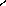
\includegraphics[width = 4cm]{crop.pdf}\hspace{\stretch{1}}
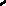
\includegraphics[width = 4cm]{crop_005.pdf}\hspace{\stretch{1}}
\caption{Comparison of virtual complexity and standard complexity}\label{f_virtualComplexity}
\end{figure}


\begin{defi}\label{DefRegSReg}
A Fermi--Ulam model is \emph{regular at infinity} if
\begin{align*}
\limsup_{k\to\infty} \frac{\LC_k(\Delta)}{\Lambda_\Delta^k}=0
\end{align*}
where $\Lambda_\Delta$ is the expansion of the limiting map $\nf_\Delta$ defined by~\eqref{DefLambdaDelta}.

A model is \emph{superregular at infinity} if there exists a constant $C$ so that for any $k\in\bN$ we have $\LC_k(\Delta)\le C$.
\end{defi}

\begin{rema}\label{RkDeltaHalf}
We will show in Appendix~\ref{AppRegInf} that for all except possibly countably many $\Delta$, the map $\nf_\Delta$ is superregular at infinity. However, the result of Appendix~\ref{AppRegInf} does not make it easy to check that a given value of $\Delta$ is regular. On the other hand~\eqref{VirtCompTrivial} shows that $\nf_\Delta$ is regular at infinity provided that $\Lambda_\Delta>2$, that is, if $|\Delta|>\frac{1}{2}$ (see~\eqref{DefLambdaDelta}).
\end{rema}

Recall that the involution defined in \S\ref{SSInvolution} conjugates $\cm^{-1}$ to the Poincaré map of the time reversed Fermi--Ulam Model corresponding to $\bar{\ell}(r)=\ell(1-r)$. Note that the parameter $\Delta$ defined by~\eqref{DefDelta} is the same for $\ell$ and $\bar{\ell}$. In particular, the Fermi--Ulam Model is regular at infinity if and only if the reversed model is regular at infinity. Therefore all results of this section formulated for unstable curves of $\cm$ are valid also for stable curves of $\cm$ (that are unstable curves of $\cm\inv$).


\subsection{Expansion estimate}\label{SSEe}
In order to properly formulate the main result of this section we need some definitions. Let $W$ be an unstable curve; then $\cm W$ (resp. $\cmp W$) consists of a (finite or) countable union of connected components. Recall that any such component may in principle be further cut by auxiliary singularities in a countable number of shorter curves which we call \emph{\Hcomps{}}.

We denote by $\{W_{i,n}\}_{i\,\in\,\bN}$ (resp. $\{\widehat W_{i,n}\}_{i\,\in\,\bN}$) the \Hcomps{} of $\cm^n W$ (resp. $\cmp^n W$). Given an \Hcomp{} $\widehat W_{i,n}$ of $\cmp^n W$, we can uniquely define $\Np_{i,n} > 0$ so that
\begin{align*}
\cmp^n|_{\cmp^{-n} \hat W_{i,n}} = \cm^{\Np_{i,n}}|_{\cmp^{-n} \hat W_{i,n}}.
\end{align*}
Finally, we denote by $\Lambda_{i,n}$ (resp. $\hat\Lambda_{i,n}$) the minimum expansion, with respect to the $\admName$-metric, of $\cm^n$ (resp. $\cmp^n$) on $\cm^{-n} W_{i,n}$ (resp. $\cmp^{-n}\widehat W_{i,n}$). Given an unstable curve $W\subset \csp$ (resp. $W\subset\cspi$), and $n > 0$, we define:
\begin{align*}
\cL_{n}(W) &= \sum_{i}\frac1{\Lambda_{i,n}},&
\hat \cL_{n}(W) &= \sum_{i}\frac1{\hat\Lambda_{i,n}}.
\end{align*}
Then we let
\begin{align*}
\cL_{n}(\delta) &= \sup_{W:|W|\adm\,\le\,\delta} \cL_{n}(W),&
\hat \cL_{n}(\delta) &= \sup_{W:|W|\adm\,\le\,\delta} \hat \cL_{n}(W),\\
\cL_{n} &= \lim_{\delta\to 0}\cL_{n}(\delta),&
\hat \cL_{n} &= \lim_{\delta\to 0} \hat \cL_{n}(\delta)
\end{align*}
(the limits in the last line exist since $\cL_n$ and $\hat\cL_n$ are decreasing functions of $\delta$). It follows from the definition that $\cL_{n}$ (resp. $\hat\cL_{n}$) is a sub-multiplicative sequence, i.e.
\begin{align}\label{eq:cL-submultiplicative}
\cL_{n+m}&\le\cL_{n}\cL_{m} & \hat\cL_{n+m}&\le\hat\cL_{n}\hat\cL_{m}.
\end{align}

\begin{prop}[Expansion estimate]\label{p_expansionEstimate}
There exists $C > 0$ such that
\begin{align}\label{e_expansionEstimate-trivial}
\hat \cL_{1} < C.
\end{align}
Moreover, if the Fermi--Ulam model is regular at infinity then there exists $\bar n > 0$ so that
\begin{align}\label{e_expansionEstimate}
\hat \cL_{\bar n} < 1,
\end{align}
and there exists $C' > 0$ so that for any $n > 0$ we have $\hat \cL_{n} < C'$.
\end{prop}

The rest of this section is devoted to the proof of Proposition~\ref{p_expansionEstimate}. We will follow the strategy described in~\cite{jmogy}. Recall the definition of the homogeneity strips $\homo_k$ given in \S\ref{s_homo}.

\begin{defi}
Let $W$ be an unstable curve. An \Hcomp{} $W_{i,n}$ (resp. $\hat W_{i,n}$) of $\cm^n W$ (resp. $\cmp^n W$) is said to be
\emph{regular} if for any $0 \le q < n$ (resp. $0\le q < \Np_{i,n}$) we have that $\cm^{-q}W_{i,n}\subset \homo_0$ (resp. $\cm^{-q}\hat W_{i,n}\subset \homo_0$) and \emph{nearly grazing} otherwise.
\end{defi}

Observe that the notion of regularity depends on the choice of the constant $k_0$ introduced in \S\ref{s_homo}; in particular, the number of regular \Hcomps{} is a non-decreasing function of $k_{0}$.
\begin{lemm}\label{l_atMostOne1}
Let $W$ be a u-curve and $N > 0$. Then any connected component of $\cm^NW$ (resp. $\cmp^NW$) contains at most one regular \Hcomp{}.
\end{lemm}
\begin{proof}
Let us first prove the statement for connected components of $\cm^NW.$ We give a proof by induction on $N$. The statement is true if $N = 1$. Indeed, the intersection of any connected u-curve with $\homo_0$ is necessarily connected, hence out of the \Hcomps{} in which a connected component of $\cm W$ is cut by secondary singularities, at most one can be regular.

Assume now by induction that the statement holds for $N$, and let $\widetilde W'$ be a connected component of $\cm^{N+1}W$. Let $\widetilde W$ be the connected component of $\cm^N W$ which contains $\cm\inv \widetilde W'$. By inductive hypothesis, either $\widetilde W$ contains no regular \Hcomp{} (and thus so does $\widetilde W'$ and the statement holds), or it contains only one regular \Hcomp{}, which we denote by $W^*\subset\widetilde W$. Then any regular \Hcomp{} of $\widetilde W'$ has to be contained in the connected u-curve $\cm W^*\cap \widetilde W'$. Since at most one of the \Hcomps{} of this curve can be contained in $\homo_0$ (and thus can be regular), we conclude the proof for $N+1$.

Finally, the statement for $\cmp^NW$ follows from the statement for $\cm^NW$. Namely, suppose that for some $N,$ $\cmp^N W$ contains two regular H-components. Denote their preimages by $W'$ and $W''$. Then $\cmp^N W'=\cm^{N'} W'$ and $\cmp^N W''=\cm^{N''} W''$. Suppose without loss of generality that $N'\leq N''$ then $\cm^{N'} W$ has two regular H-components giving the contradiction.
\end{proof}

\begin{defi}\label{d_regularComplexity}
Given an unstable curve $W$ and $n > 0$, we define the \emph{regular $n$-complexity} of $W$ (resp. the \emph{induced regular $n$-complexity} of $W$), denoted by $\kreg_n(W)$ (resp. $\hkreg_n(W)$) to be the number of regular \Hcomps{} of $\cm^nW$ (resp. $\cmp^n W$). If $n = 0$ we set conventionally $\kreg_0(W) = \hkreg_0(W) = 1$. Finally, define
\begin{align*}
\kreg_n(\delta) &= \sup_{W:|W|\adm\,\le\,\delta}\kreg_n(W),&
\hkreg_n(\delta) &= \sup_{W:|W|\adm\,\le\,\delta}\hkreg_n(W);\\
\kreg_n &= \lim_{\delta\to0}\kreg_n(\delta),&
\hkreg_n &= \lim_{\delta\to0}\hkreg_n(\delta)
\end{align*}
\end{defi}

(as before the limits in the last line exist by monotonicity).
\begin{rema}


Given an unstable curve $W$, recall the standard definition of $n$-\emph{complexity} of $W$ as the number of connected components of $\cm^nW$. Lemma~\ref{l_atMostOne1} implies that regular complexity does not exceed standard complexity. Observe moreover that while standard complexity is non-{}decreasing in $n$, regular complexity is not necessarily so (e.g. the image of a regular component of $\cm^nW$ may contain no regular component). Finally, all the above quantities are non-decreasing in $k_0$.
\end{rema}

For future use, we note that Lemma~\ref{l_largeCell}$\MK$\eqref{i_almostFinite} and~\eqref{l_atMostOne1} imply that, provided $k_0$ is sufficiently large and $\delta$ is sufficiently small, the following trivial estimate holds:
\begin{align}\label{e_trivialEstimateOnRegularComplexity}
\kreg_n(\delta) &\le 3^n.
\end{align}

Let us now define $\zreg$, $\hzreg$ (resp. $\cL^{*}, \hat \cL^{*}$) as we did above for $\cL$ and $\hat \cL$, but summing only on regular (resp. nearly grazing components). For instance:
\begin{align*}
\cL^{*}_{n} = \lim_{\delta\to0}\;\sup_{W\,:\,|W|\adm\,\le\,\delta}{\sum_i}^*\frac1{\Lambda_{i,n}},
\end{align*}
where $\sum^{*}$ denotes that the sum is restricted only to nearly grazing components. The following lemmata will allow us to prove Proposition~\ref{p_expansionEstimate}.

\begin{lemm}[Control for nearly grazing components]\label{l_nearlyGrazing}
For any $N > 0$ and $\eps > 0$, we can choose $k_0$ large enough in the definition of homogeneity strips so that $\cL_{n}^{*} < \eps\text{ for any $0 < n\le N$}$.
\end{lemm}


\begin{lemm}[Bound on regular complexity]\label{l_regularComplexityBound}
If the Fermi--Ulam model is regular at infinity, there exists $\brn > 0$ such that if $\delta$ is sufficiently small then for each~$k_0$
\begin{equation}\label{EqGlobCompl}
\hzreg_{\brn}(\delta)
\leq \frac{1}{2}.
\end{equation}
\end{lemm} The proofs of the above lemmata are independent of each other. Lemma~\ref{l_nearlyGrazing} is proved in \S\ref{SS-NG}, the proof of Lemma~\ref{l_regularComplexityBound} occupies
\S\ref{ss_regularComplexity} and~\S\ref{SSPointwise}.

Observe that Lemma~\ref{l_nearlyGrazing} allows us to prove that
\begin{align}\label{eq:cl1-bounded}
\cL_{1} < \infty.
\end{align}
In fact, $\cL_{1} = \zreg_{1}+ \cL^{*}_{1}$. By Lemma~\ref{l_nearlyGrazing}, the second term can be made as small as needed, and by Lemma~\ref{l_largeCell}$\MK$\eqref{i_almostFinite}, provided that $|W|\adm$ is small enough, the first term is at most $3\cdot \underline \Lambda\inv$, where $\underline\Lambda$ is a lower bound for~\eqref{e_expansionAdm}.

Combining these two results yields\footnote{ The proof given below is similar to the one used in~\cite[Main Theorem]{jmogy}.} the proof of the Expansion Estimate:

\begin{proof}[{Proof of Proposition~\ref{p_expansionEstimate}}]
Let $W$ be an unstable curve so that $|W|\adm < \delta$ with $\delta > 0$ sufficiently small. Recall that $\Lambda$ is the minimal expansion of $\cmp$ in the $\alpha$-metric (see~\eqref{e_uniformHyperbolicity}). Observe that by definition, for any $n > 0$
\begin{align*}
\hat \cL_{n}(W) = \hzreg_{n}(W)+\hat \cL^{*}_{n}(W).
\end{align*}


In view of Lemma~\ref{l_regularComplexityBound} it is enough to show that, if $\delta$ is sufficiently small, we have $\hat \cL^{*}_{n} < 1/2$ for all $0 < n\le\bar n$ where $\bar n$ is from Lemma~\ref{l_regularComplexityBound}. By Proposition~\ref{p_largeEnergiesFUM} there exists $\bar w = \bar w(\bar n)$ so that, if $W\subset\cspil{\bar w}$, then $\cmp^{n}W$ has no nearly grazing\linebreak \Hcomps{} for any $0 < n\le\bar n$. Since by Corollary~\ref{c_weakBoundOnEndpoint}, the velocity of the particle increases by at most $O(1)$ for each iteration of $\cmp$, we conclude that for each nearly grazing component, the maximal velocity on this component during the first $\bar n$ iterations of $\cmp$ is bounded by $\const (\bar w+\bar n).$ Now~\eqref{e_weakBoundOnNp} implies that there exists a uniform $\bar n'\sim \bar n(\bar w+\bar n)$ so that $\Np_{i,n}\le\bar n'$ for any nearly grazing \Hcomp{} $\hat W_{i, n}$. Thus
\begin{align*}
{\sum_i}^*\frac1{\hat\Lambda_{i,n}} =
\sum_{k = 1}^{\bar n'}\;{\sum_{i:\Np_{i, n} = k}}^*
\frac1{\hat\Lambda_{i, n}} \le
\sum_{k = 1}^{\bar n'}{\sum_j}^*\frac1{\Lambda_{j,k}}.
\end{align*}
Hence, it is sufficient to apply Lemma~\ref{l_nearlyGrazing} with $N = \bar n'$ and $\eps = 1/(4\bar n')$ to obtain both~\eqref{e_expansionEstimate-trivial} (with $C = K+1/2$) and~\eqref{e_expansionEstimate}.

The uniform bound on $\hat \cL_{n}$ for all $n$ follows since $\hat\cL_{m+n}\le\hat\cL_{m}\hat\cL_{n}$. Namely, let $n = p\bar n+r$, where $0\le r < \bar n$. Then
\begin{align*}
\hat\cL_{n}\le\hat\cL_{\bar n}^{p}\cdot
\hat\cL_{1}^{r}&\le C^{\bar n}.\qedhere
\end{align*}
\end{proof}
\subsection{Control of nearly grazing components}\label{SS-NG}
\begin{proof}[{Proof of Lemma~\ref{l_nearlyGrazing}}]
We prove the lemma by induction on $N$. Let us first assume $N = 1$ and let $\tilde W'$ be a connected component (rather than an \Hcomp{}) of $\cm W$. If we restrict to $H$-components contained in $\tilde W'$, then by~\eqref{e_expansionAdm-II} we obtain
\begin{align*}
{\sum_i}^*\frac{1}{\Lambda_{i,1}} &\le\sum_{k\,\ge\,k_0}\const k_0^{-2} = \const k_0\inv.
\end{align*}
Were the number of connected components $\tilde W'_i$ of $\cm W$
\emph{uniformly bounded}, our claim would thus be proved. As we already observed, this is not the case. Fix $n_*$ sufficiently large. Lemma~\ref{l_largeCell}$\MK$\eqref{i_almostFinite} ensures that, except for finitely many (i.e. $3$) connected components of $\cm W$, all the others will intersect cells $\cell^-_\indCell$ with $\indCell\ge n_*$. Moreover, by Lemma~\ref{l_singularityStructure}$\MK$\eqref{i_boundedCells}
%~\ref{l_largeCell}(b),
$\cell^-_\indCell$ will intersect only homogeneity strips $\homo_k$ for $k > \const \indCell^{1/4}$. Denote by $W_{[\indCell,k],1}$ the $H$-component of $\cm W$ such that $W_{[\indCell,k],1}\subset\homo_k\cap\cell^-_\indCell$. Then using~\eqref{e_expansionAuxMetricB}, estimating the flight time by $\indCell$ and the relative velocity by $k^{-2}$ we conclude that the expansion of $W_{[\indCell,k],1}$ satisfies
\begin{align*}
\Lambda_{[\indCell,k],1} > \const \indCell k^2.
\end{align*}
We thus gather that, if $n_*$ is sufficiently large and $W$ is sufficiently short, then
\begin{align*}
{\sum_{i}}^*\frac1{\Lambda_{i,1}} &\le \const k_0\inv + \sum_{\indCell\,\ge\,n_*}
\;\sum_{k\,\ge\,\const \indCell^{1/4}}\frac1{\Lambda_{[\indCell,k],1}}\\%
&\le \const k_0\inv + \sum_{\indCell\,\ge\,n_*} \const \indCell^{-5/4}\le\const \left(k_0\inv + n_*^{-1/4}\right).
\end{align*}
The last expression can then be made as small as needed by choosing $k_0$ and $n_*$ sufficiently large. We thus obtained our base step: for any $\eps > 0$, if $k_0$ is sufficiently large we have $\DS
\cL_{1} < \eps. $

Using the above notation, we assume by inductive hypothesis that for any $\eps > 0$ we can choose $k_0$ large enough in the definition of homogeneity strips so that $\cL_{n}^{*} < \eps$ and we want to show that $\cL_{n+1}^{*} < \eps$. In order to prove the inductive step, observe that for any u-curve $W$, we have the following inductive relation summing over the H-components $W_{i,1}$ of $\cm W$:
\begin{align}\label{e_inductivecL}
\cL_{n+1}^*(W) &\le \sum_{i:\:W_{i,1}\text{ is reg.}}\frac1{\Lambda_{i,1}}\cL^*_{n}(W_{i,1}) + {\sum_{i}}^*\frac1{\Lambda_{i,1}}\cL_{n}(W_{i,1}).
\end{align}

By Proposition~\ref{p_propertiesAdm}$\MK$\eqref{i_expansionAdm}, there exists $0 < \LambdaMin < 1$ so that $\Lambda_{i,n} > \LambdaMin^n$ for any $n > 0$. Thus, for any $\delta\in(0,1)$ sufficiently small, \eqref{e_trivialEstimateOnRegularComplexity} and our inductive assumption imply the following rough bound on $\cL_{n}(\delta)$:
\begin{align}\label{RoughL}
\cL_n(\delta) \le
\frac{3^n}{\LambdaMin^n}+\cL_n^*(\delta)\le 2\frac{3^n}{\LambdaMin^n}.
\end{align}
Using Lemma~\ref{l_globalExpansion}$\MK$(a) we get that if $|W|\adm < \delta$, then $|W_{i,1}|\adm < C_*\delta^{1/4}$. Hence by~\eqref{e_inductivecL} and using once again~\eqref{e_trivialEstimateOnRegularComplexity}, if $|W|\adm < \delta$:
\begin{align*}
\cL_{n+1}^*(\delta) &\le \sum_{i:\:W_{i,1}\text{ is reg.}}\frac1{\Lambda_{i,1}}\cL^*_{n}\left(C_*\delta^{1/4}\right) + {\sum_{i}}^*\frac1{\Lambda_{i,1}}\cL_{n}\left(C_*\delta^{1/4}\right)\\
&\le \frac{3}{\LambdaMin}\cL_{n}^*\left(C_*\delta^{1/4}\right)+\cL^*_1(W)\cL_{n}\left(C_*\delta^{1/4}\right).
\end{align*}
Using the inductive hypothesis and~\eqref{RoughL}, taking $\liminf_{\delta\to0}$ we gather that $\cL_{n+1}^* < \Const \eps$, which concludes the proof of the inductive step.
\end{proof}
\subsection{Control on regular complexity}\label{ss_regularComplexity}
In this section we prove that we can bound the induced regular complexity $\hkreg_n$, needed to prove Lemma~\ref{l_regularComplexityBound}, by means of two other quantities. One is the virtual complexity introduced in Subsection~\ref{SS-VirtualComplexity} and the other is the
\emph{pointwise complexity}, which we now proceed to define.

Let $x\in\csp$ and let $Q_n$ be a connected component of $\csp\setminus\sing n$ so that $\cl Q_n\ni x$. We say that $Q_n$ is
\emph{$n$-regular at $x$} if
\begin{align*}
\lim_{Q_n\,\ni\,x'\to x}\cm^{l}x'\in \cl\homo_0\text{ for all $0 < l\le n$};
\end{align*}
otherwise $Q_n$ is said to be \emph{nearly grazing at $x$}.

\begin{defi}\label{d_regular pointwise complexity}
Given a point $x\in\csp$ and $n > 0$, we define the \emph{$n$-regular complexity at $x$}, denoted with $\ckreg_n(x)$, to be the number of components of $\csp\setminus\sing n$ whose closure contain $x$ and that are $n$-regular at $x$. We then define:
\begin{align*}
\ckreg_n = \sup_{x\,\in\,\csp}\ckreg_n(x).
\end{align*}
\end{defi}

Observe that also this notion of complexity is monotone with respect to $k_{0}$: by increasing $k_{0}$ we allow more components to be regular, thus the regular complexity is non-decreasing as a function of $k_{0}$.

We now proceed to define corresponding notions for the induced dynamics. Recall that $\singp{n}$ denotes the singularity set of $\cmp^{n}$ and let $\hat Q_n$ be a connected component of $\cspi\setminus\singp{n}$. By the discussion prior to Lemma~\ref{LmFRet} we conclude that there exists $\Np_n(\cc_n)$ so that for any $x\in\hat Q_n$ we have $\cmp^n(x) = \cm^{\Np_n(\cc_n)}(x)$. Suppose now that $x\in\cl\hat Q_n$; we say that $\hat Q_n$ is $n$-regular at $x$ if
\begin{align*}
\lim_{\hat Q_n\,\ni\,x'\to x}\cm^{l}x'\in \cl\homo_0\text{ for all }0 < l\le \Np_n(\cc_n).
\end{align*}
Define $\ckregp_n(x)$ to be the number of connected components of $\cspi\setminus\singp{n}$ whose closure contains $x$ and which are $n$-regular at $x$. Set
\begin{align}\label{e_defInducedRegularComplexity}
\ckregp_n = \sup_{x\,\in\,\cspi}\ckregp_n(x).
\end{align}
Once again, this notion of complexity is monotone with respect to $k_{0}$.


If the phase space $\csp$ were compact (as it is in the case of dispersing billiards) then $\kregp_n$ (see Definition~\ref{d_regularComplexity}) and $\ckregp_n$ would coincide (see case (a) in the proof of Lemma~\ref{LmCInf-EE} below). Since our phase space is not compact, we need a more careful analysis.

\begin{lemm} \label{LmCInf-EE}
Suppose that there exists $\bar n > 0$ so that for each choice of $k_{0}$:
\begin{equation}\label{e_boundAssumption}
\ckregp_{\bar n}< \frac{\Lambda^{\bar n}}{2} \text{ and }
\LC_{\bar n}(\Delta)\leq \frac{\hat C\Lambda_\Delta^{\bar n}}{4}
\end{equation}
where $\Lambda$ is the minimal expansion in $\alpha$-metric, $\Lambda_\Delta$ is the expansion of the limiting map, defined by~\eqref{DefLambdaDelta}, and $ \hat C$ is from Corollary~\ref{CrExpAtInf}, then there exists $\delta$ so that~\eqref{EqGlobCompl} holds.
\end{lemm}

\begin{proof}
Assume by contradiction that for any $n$ and any $\delta_{0}$ there exists $0 < \delta < \delta_{0}$ so that
\begin{align*}
{\hzreg_{n}}(\delta) > \frac12.
\end{align*}
In particular, for $n = \brn$, there exists a sequence $(\Wseq{m})_{m\,>\,0}$ of unstable curves so that $|\Wseq{m}|\adm\to 0$ as $m\to\infty$ and $\hzreg_{\brn}(\Wseq{m}) > \frac{1}{2}$ for any $m > 0$. Observe that
\begin{align}\label{LGeneralBound}
\hzreg_{\brn}(W)\le \frac{\hkreg_{\brn}(W)}{\min_{i} \Lambda_{i, \brn}}.
\end{align}
Pick arbitrary points $x^{(m)}\in \Wseq{m}$. After possibly passing to a subsequence we can assume that one of the two possibilities below hold.
\begin{enumerate}\alphenumi
\item the sequence $x^{(m)}$ is bounded;
\item the sequence $x^{(m)}$ tends to infinity.
\end{enumerate}

We analyze these two cases separately.

\begin{case}
In this case we estimate the denominator of~\eqref{LGeneralBound} by $\Lambda^{\brn}$ obtaining
\begin{align}\label{eq:contradiction-small-w}
\hkreg_{\brn}(W) > \frac{\Lambda^{\brn}}{2}.
\end{align}

Since the sequence $x^{(m)}$ is bounded, combining~\eqref{e_trivialEstimateOnRegularComplexity} with~\eqref{e_weakBoundOnNp} we gather that $(\hkreg_{\brn}(\Wseq{m}))_{m\,>\,0}$ is also a bounded sequence. We can therefore assume (possibly passing to a subsequence) that $\hkreg_{\brn}(\Wseq{m}) = \Kn $ for all $m$.

As noted earlier, the set $\cspi\setminus\singp{\brn}$ is the union of a countable number of connected components. By Lemmata~\ref{l_singularityStructure} and~\ref{LmFRet}, to each such component\footnote{We drop the subscript $\brn$ as this is fixed once and for all and will not cause any confusion.} $\cc$ we can uniquely associate a $\Np_{\brn}(\cc)$-tuple
\begin{align*}
\indTuple(\cc) = \left(\indCell_0,\indCell_1,\cdots,\indCell_{\Np_{\brn}(\cc)-1}\right)
\textrm{ where } \indCell_i\in\{\recoPrivate,0,1,\cdots\}
\end{align*}
so that
\begin{align*}
\cc = \cspi \cap \bigcap_{l = 0}^{\Np(\cc)-1}\cm^{-l}\cell^+_{\indCell_l}.
\end{align*}
For $0\le i < \Kn$, denote by $\Wseq{m}_i$ the preimage under $\cmp^{\brn}$ of the $i^{\,\rm th}$ regular \Hcomp{} of $\cmp^{\brn}\Wseq m$. Let $\ccseq{m}_i$ be so that $\Wseq{m}_i\subset\ccseq{m}_i$: notice that by Lemma~\ref{l_atMostOne1}, $\ccseq{m}_i\ne\ccseq{m}_j$ if $i\ne j$.

Since $\cmp^{\brn}\Wseq{m}_i$ is regular, there exists some $\redCell > 0$ (depending on $k_{0}$) so that $\indCell_l(\ccseq{m}_{i}) \in\{\recoPrivate,0,1,\cdots,\redCell\}$ for all $0 < l \le \Np_{\brn}(\ccseq{m}_{i})$. Since the sequence $(\Wseq{m})_m$ is bounded, we conclude by~\eqref{e_weakBoundOnNp} that $(\Np_{\brn}(\ccseq{m}_i))_{m}$ is also a bounded sequence.

Since there are only finitely many $\cc$'s which satisfy these requirements, we can always assume (extracting a subsequence if necessary) that $\ccseq{m}_i = \ccseq{m'}_i$ for any $m,m'$; for ease of notation we will denote such connected components simply by $\cc_i$.

Let us now choose arbitrarily points $\xseq{m}_i\in\Wseq{m}_i\subset\cc_i$. Since $(\xseq{m}_i)_m$ is a bounded sequence, we can assume (extracting a subsequence if necessary) that $\xseq{m}_i\to\bar x_i$ for some $\bar x_i\in\cl\cc_i$. On the other hand, since $|\Wseq{m}|\adm\to0$ and $|\cdot|\adm$ is equivalent to the Euclidean norm if $w$ is bounded, it must be that $\bar x_i = \bar x_j$ for every $0\le i,j < \Kn $. We call this common limit point $\bar x$.

Since $\cmp^{\brn}\Wseq{m}_i$ is regular, we conclude that each of the $\cc_i$'s is regular at $\bar x$. We conclude that $\Kn \leq \ckregp_{\bar n}(\bar x)\leq \ckregp_{\bar n}$, which contradicts~\eqref{eq:contradiction-small-w} by the first estimate in~\eqref{e_boundAssumption}.
\end{case}

\begin{case}
In this case we estimate the denominator of~\eqref{LGeneralBound} using Corollary~\ref{CrExpAtInf}; note that since $x^{(m)}$ tends to infinity, we can always assume that $w > \law{}(\bar n)$ holds, where $\law{}(\cdot)$ is obtained in Corollary~\ref{CrExpAtInf}. We thus obtain
\begin{align*}
\hzreg_{\brn}(W) \leq \frac{\hkreg_{\brn}(W)}{\hat{C}_{\Delta} \Lambda_\Delta^{\brn}}.
\end{align*}

Observe that if we show $\hkreg_{\bar n}(W^{(m)}) \leq 2\LC_{\bar n}(\Delta)$ for all but finitely many $m$'s, then~\eqref{EqGlobCompl} follows from the second estimate in~\eqref{e_boundAssumption}. We proceed by contradiction and assume (possibly extracting a subsequence) that $|\Wseq{m}|\adm\to 0$, $ \min_{\Wseq{m}} w\to\infty$, but
\begin{align*}
\hkreg_{\bar n}(\Wseq{m})\geq 2\LC_{\bar n}(\Delta)+1 \text{ for all }m > 0.
\end{align*}
Recall the definition (see~\eqref{e_fundamentalDomains}) of the fundamental domains $\Dom_n\!\!=\! \{x\!\in\!\cspi\st \Np(x) = n\}$. Similarly to~\eqref{DefItin}, we define, for $k > 0$:
\begin{align*}
\Dom_{n_0,n_1,\cdots,n_{k-1}} &= \bigcap_{j = 0}^{k-1}\cmp^{-j}\Dom_{n_j}.
\end{align*}
A $k$-tuple $(n_0,n_1,\!\cdots\!,n_{k-1})$ is said to be
\emph{$\cmp$-admissible} if $\Dom_{n_0,n_1,\cdots,n_{k-1}}\!\!\ne\!\emptyset$. If $x\in\Dom_{n_0,n_1,\cdots,n_{k-1}}$, we say that $(n_0,n_1,\cdots,n_{k-1})$ is the\footnote{In
\S\ref{SS-VirtualComplexity} we gave similar definitions for domains given in terms of the normal form. It must be noted that here we do not take the closure in the definition of the $\Dom_{n_0,n_1,\cdots,n_{k-1}}$'s, hence we can define \emph{the} itinerary (as opposed as \emph{an} itinerary) of a point $x$. The reason for this mismatch is that the $\Dom_n$'s are defined dynamically (as opposed to the geometric definition of $\hDom_n$), and thus their boundary carry some dynamical information which we want to preserve.} 
\emph{$k$-itinerary} of $x$. Define a sequence $(N_m)_m$ so that $\Wpseq{m} \!\!:= \Wseq{m}\cap D_{N_m}\ne\emptyset$ and $\hkreg_{\bar n}(\Wpseq{m})\ge \LC_{\bar n}(\Delta)+1$. Such a sequence exists since any sufficiently short unstable curve intersects at most two domains $D_N$. Passing to the $(\tau, I)$-coordinates and taking a subsequence we may assume that $T_{-N_m} \Wpseq{m}$ converges to some point $\brx\in \cl(\hDom_0)$, where $T_n$ is the translation map defined in~\eqref{e_translationMapDefinition}. The convergence in the $\admName$-metric implies convergence in the $(\tau,I)$-Euclidean metric by~\eqref{e_boundAlphaTau}.

Since $\cmp^{\bar n}$ is continuous on the set of points with a given itinerary, it follows that there are points $\xseq{m}_1, \xseq{m}_2\dots \xseq{m}_{\LC_{\bar n}(\Delta)+1}\in
\Wpseq{m}$ having different $k$-itineraries. Possibly by extracting a subsequence, we may thus assume that for $1\le l\le\LC_{\bar n}(\Delta)+1$
\begin{align*}
\xseq{m}_{l}\in D_{N_m, N_m+n_{1,l}\dots N_m+n_{\bar n-1,l}},
\end{align*}
that is, that the itinerary depends on $N_m$ only via the shift by $N_m$. But then, Theorem~\ref{t_normalForm} implies that $\brx\in \hDom_{0, n_{1,l}\dots n_{\bar n-1,l}}$ for every $l$, therefore $\LC_{\bar n}(\brx)\geq \LC_{\bar n}(\Delta)+1$, which contradicts the definition of $\LC_{\bar n}(\Delta)$.\qedhere
\end{case}\let\qed\relax
\end{proof}



\subsection{Linear bound on regular complexity.}\label{SSPointwise}

In this section we prove a linear bound for $\ckregp_n$ defined by~\eqref{e_defInducedRegularComplexity}.

\begin{lemm}\label{l_actualInducedComplexityBound}
For any $n > 0$ we have, independently on $k_{0}$:
\begin{align}\label{e_actualInducedComplexityBound}
\ckregp_n < 4n + 2.
\end{align}
\end{lemm} 

The above lemma is the key result used to prove Lemma~\ref{l_regularComplexityBound}.

\begin{proof}[Proof of Lemma~\ref{l_regularComplexityBound}]
By Lemma~\ref{l_actualInducedComplexityBound}, we can find $n^{*}$ so that for any $\bar n > n^*$ we have $4\bar n+2\leq \Lambda^{\bar n}/2$. Since the Fermi--Ulam Model is regular at infinity (Definition~\ref{DefRegSReg}), we conclude that for $\bar n$ sufficiently large (and larger than $n^{*}$) the second condition in~\eqref{e_boundAssumption} holds. Lemma~\ref{l_regularComplexityBound} follows.
\end{proof}

The induced regular complexity $\ckregp_n$ bounds the number of connected components of $\cspi\setminus\singp{n}$ that are regular at any point $x$. Since such connected components are bounded by $C^{1}$ curves, it is possible to formulate an equivalent infinitesimal definition, which we now describe.

For $x\in\csp$, denote by $\tangu_x\csp$ the unit tangent circle at $x$. We identify each element of $u\in\tangu_{x}\csp$ with the equivalence class of $C^1$-curves in $\csp$ which emanate from $x$ with a tangent vector that is a positive multiple of $u$. Of course $\tangu_x\csp$ embeds naturally in $\tang_x\csp$; this embedding defines a topology on $\tangu_x\csp$. Observe that if $x\in\intr\csp$, then $\tangu_x\csp = \hhs^1$, but if $x\in\sing0$, then $\tangu_x\csp$ is a closed quarter-circle if $x = (0,0)$ or $x = (1,0)$ and a closed half-circle otherwise. All such sets will be considered with the counterclockwise orientation. Similarly, we define, for any $x\in\cspi$, the set $\tangu_x\cspi$.

A $C^1$-curve in $\csp$ emanating from $x$ thus naturally induces an element of $\tangu_x\csp$. In particular if $x\in\sing n$, then the curves in $\sing n$ cut $\tangu_x\csp$ into a number of connected components which we call \emph{tangent sectors}. With a slight abuse of notation we write $\tangu_x\csp\setminus\sing n$ to denote $\tangu_{x}\csp\setminus\{u_1,\cdots,u_{p}\}$ where the $u_i$'s are the unit vectors induced by the curves of $\sing{n}$ which meet at $x$. Similar considerations apply to $\cspi$~and~$\singp n$.

More generally, given two elements $u_-\!\!\ne \!\!u_+\in\tangu_x\csp$ let $\cV=\cV(u_-, u_+)$ denote the set of directions lying between $u_-$ and $u_+$ with respect to the counterclockwise orientation. This set will be called the \emph{tangent sector centered at $x$ bounded by $u_-$ and $u_+$}. Conventionally, we also introduce the notion of \emph{empty sector} $\cV = \emptyset$ and \emph{full sector} $\cV = \tangu_{x}\csp$. A curve $\Gamma$ which emanates from $x$ with unit tangent vector $u\in\cV$ is said to be \emph{compatible} with $\cV$.

\noindent Note that all sufficiently short curves compatible with $\cV\subset\tangu_{x}(\csp\setminus\sing n)$ necessarily belong to the same connected component $Q_n$. Likewise, all sufficiently short curves compatible with $\cV\subset\tangu_{x}(\cspi\setminus\singp n)$ necessarily belong to the same connected component $\hat Q_n = \hat Q_n(\cV)$. We denote $\Np_n(\cV) = \Np_n(\hat Q_n(\cV))$.

Let $\cV\subset\tangu_{x}(\csp\setminus\sing n)$ and $\Gamma$ be a curve compatible with $\cV$. By construction we have that $\lim_{\Gamma\,\ni\,x'\to x}\cm^l x'$ is well defined and independent of $\Gamma$ for any $0\le l\le n$. Let us denote this limit point $x^l_\cV$. Likewise, if $\cV\subset\tangu_{x}(\cspi\setminus\singp n)$, we can uniquely define $x^{l}_{\cV}$ for any $0\le l\le \Np_n(\cV)$.

Let $\cV\subset\tangu_{x}(\csp\setminus\sing n)$. We can define for any $0\le l\le n$ the image sector
\[
\cV^l\subset\tangu_{x^{l}_{\cV}}\left(\csp\setminus\sing{-l,n-l}\right)
\]
as follows. Let $\Gamma$ be a curve compatible with $\cV$. By construction
$\lim_{\Gamma\,\ni\,x'\to x}D_{x'}\cm^l$ is a well defined linear map independent of the choice of $\Gamma$ for any $0\le l\le n$. We denote its action on 
$\tangu_x\csp$ by 
\[
\cm_{x,\cV*}^{l}:\tangu_x\csp\to\tangu_{x^{l}_{\cV}}\csp.
\]
Then, with an abuse of notation we denote with $\cm^{l}_{*}\cV$ the sector $\cm^{l}_{x,\cV*}\cV$. A similar construction yields, for any $\cV\subset\tangu_{x}\cspi\setminus\singp n$ and any $0\le l\le n$ the definition of
\[
\cmp^{l}_{*}\cV\subset\tangu_{x^{\Np_l(\cV)}_{\cV}}\left(\cspi\setminus\singp{-l,n-l}\right).
\]

A tangent sector $\cV\subset\tangu_{x}\csp\setminus\sing n$ is said to be \emph{$\cm^n$-regular} if it is non-empty and $x_\cV^{l}\in\cl\homo_0$ for any $0 < l\le n$. Otherwise, we say that the sector is \emph{nearly grazing}. Likewise, a tangent sector $\cV\subset\tangu_{x}(\cspi\setminus\singp n)$ is said to be
\emph{$\cmp^n$-regular} if it is non-empty and $x_\cV^{l}\in\cl\homo_0$ for any $0 < l\le \Np_n(\cV)$.

Of course the above definitions are compatible with the ones given previously for $Q_n$ and $\hat Q_n$ in the sense that a sector $\cV\in\tangu_x(\csp\setminus\sing n)$ is $\cm^{n}$-regular if and only if the corresponding connected component $Q_n$ is $n$-regular at $x$, and a sector $\cV\in\tangu_x(\cspi\setminus\singp n)$ is $\cmp^{n}$-regular if and only if the corresponding connected component $\hat Q_n$ is $n$-regular at $x$. This immediately follows by our construction unless the connected component joins $x$ with a cusp (i.e. the corresponding sector is empty). But then we claim that the component must necessarily be nearly grazing at $x$. In fact, it is easy to see that if the sector generated by a connected component $\hat Q_n$ is degenerate, then there exists $0 < l\le \Np_n(\hat Q_n)$ so that $D\cm^l|_{\hat Q_n}$ is singular as we approach $x$. Since $D\cm$ is singular only at $\{w = 0\}$, $\hat Q_n$ cannot be regular at $x$.

In particular, the regular complexity $\ckreg_n$ is the maximum number of $\cm^{n}$-regular sectors in which $\sing n$ cuts $\tangu_x\csp$ for any $x\in\csp$. The corresponding statement holds true for $\ckregp_n$.



\begin{defi}\label{d_goodSector}
A tangent sector $\cV(u_-,u_+)\subset\tangu_x\csp$ (or $\cV(u_-,u_+)\subset\tangu_x\cspi$) is said to be
\emph{good} if
\begin{enumerate}\romanenumi
\item\label{i_decreasingVectors}
$u_{+},u_-\in\conen_x$ (recall definition~\eqref{e_definitionClosedConesB}) and
\item\label{i_sectorPi}
the angle between $u_{-}$ and $u_+$ does not exceed $\pi$.
\end{enumerate}

A good tangent sector $\cV(u_-,u_+)$ is said to be
\emph{active} if $u_-$ and $u_+$ belong to different quadrants, and \emph{inactive} if they belong to the same quadrant.
\end{defi}

Observe that an active good sector contains either the first or the third quadrant (in particular, the stable cone); inactive sectors { do not intersect these} quadrants. In particular, since future singularities are unions of stable curves (Lemma~\ref{l_localSing}), if a good sector $\cV\subset\tangu_{x}\csp$ (resp. $\cV\subset\tangu_{x}\cspi$) is inactive, then for any $k > 0$ we have $\cV\subset\tangu_{x}(\csp\setminus\sing k)$ (resp. $\cV\subset\tangu_{x}(\cspi\setminus\sing k)$).

Good sectors satisfy the following invariance property.


\begin{lemm}\label{l_invarianceGoodSectors}
Let $\cV\subset\tangu_{x}\csp$ be a good sector, and $\cV\setminus\sing 1 = \bigcup_{i = 1}^{s}\cV_{i}$. Then each image sector $\cm_{*}\cV_{i}$ is good. Similarly, if $\cV\subset\tangu_{x}\cspi$, and $\cV\setminus\singp1 = \bigcup_{i = 1}^{s}\cV_{i}$, we have that each image sector $\cmp_{*}\cV_i$ is a good sector.
\end{lemm}

\begin{proof}
First of all observe that the image by a linear map of a sector of angle at most $\pi$ is a sector of angle at most $\pi$. We conclude that item~\eqref{i_sectorPi} in Definition~\ref{d_goodSector} holds for each of the image sectors.

Let $u$ be one of the boundary vectors of $\cV_{i}$. There are two possibilities: either $u$ is one of the boundary vectors of $\cV$, or it is induced by $\sing1$. In the first case, $u\in\conen_{x}$ and thus~\eqref{e_decreasingCone} implies that its image $\cm_{\cV_{i}*}u\in\coneu_{\cm_{\cV_{i}}x}\subset\conen_{\cm_{\cV_{i}}x}$. In the second case, we have by construction that $\cm_{\cV_{i}*} u$ is tangent to some curve in $\sing{-1}$. Lemma~\ref{l_localSing} then implies that also in this case $\cm_{\cV_{i},*}u \in\conen_{\cm_{\cV_{i}}x}$, which concludes the proof of the first part. The second part follows from identical considerations.
\end{proof}
\begin{rema}
Lemma~\ref{l_invarianceGoodSectors} implies in particular that if $\cV\subset\tangu_x(\csp\setminus\sing k)$ is a good sector, then $\cm^l_{*}\cV$ is also a good sector for any $0\le l\le k$.
\end{rema}

The linear bound~\eqref{e_actualInducedComplexityBound} will be obtained by means of the following lemma, whose proof we briefly postpone.

\pagebreak
\begin{lemm}\label{l_inductiveStep}
\leavevmode
\begin{enumerate}\alphenumi
\item \label{i_inductiveStep}
Let $x\in\csp\setminus\{\xc\}$. Any active good tangent sector $\cV\subset\tangu_x\csp$ is cut by $\sing1$ in at most two $\cm$-regular sectors. The $\cm$-image of at most one of them is active.
\item \label{i_inducedInductiveStep}
Let $x\in\cspi\setminus\{\xc\}$. Any active good tangent sector $\cV\subset\tangu_x\cspi$ is cut by $\singp1$ in at most three $\cmp$-regular sectors. The $\cmp$-image of at most one of them is active.
\end{enumerate}
\end{lemm} 

We can now prove the main result of this subsection.
\begin{proof}[{Proof of Lemma~\ref{l_actualInducedComplexityBound}}]
First observe that Lemma~\ref{l_continuityAtxc} implies that if $x$ is sufficiently close to $\xc$, then $\cm x$ is also close to $\xc$, which implies that $\Np(x) = 1$ and that $\cmp x\nin\homo_0$. Hence, no sector $\cV\subset\tangu_x\cspi$ can be $\cmp$-regular. We can thus assume $x\in\cspi\setminus\{\xc\}$.

Cutting $\tangu_x\cspi$ along the vertical direction we obtain (up to) $2$ good sectors (recall Remark~\ref{r_boundary cspi}); of course both sectors might be active.

Let $\cV$ denote one such active sector. We now show inductively that for any $k > 0$, the singularity set $\singp{k}$ cuts $\cV$ in at most $(2k+1)$ $\cmp^{k}$-regular sectors, and the $\cmp^{k}$-image of at most one of them is active. Lemma~\ref{l_inductiveStep}$\MK$\eqref{i_inducedInductiveStep} proves our claim for $k = 1$. In order to proceed with our proof, we need to set up some notation: for any $k\ge 1$, the singularity set $\singp {k}$ cuts $\cV$ in a number $s_{k}$ of sectors $(\cV^{(k)}_0,\cV^{(k)}_1,\cdots,\cV^{(k)}_{s_{k}-1})$; let $r_k$ denote the number of such sectors that are $\cmp^{k}$-regular. Without loss of generality we can take them to be $(\cV^{(k)}_0,\cV^{(k)}_1,\cdots,\cV^{(k)}_{r_k-1})$.

Assume now, by induction, that our claim holds for $k$; we gather that $r_k\le {2}k+1$ and that the image of at most one of the regular sectors is active. If no sector is active, no further cutting is allowed, so we are done. Hence we assume that one sector is active and without loss of generality we let it be indexed as $\cV^{(k)}_0$.

Consider now the $\cmp^{k+1}$-regular sectors $(\cV^{(k+1)}_0,\cV^{(k+1)}_1,\cdots,\cV^{(k+1)}_{r_{k+1}-1})$ obtained by cutting $\cV$ by $\singp{k+1}$. By definition of $\cmp^{k+1}$-regularity, for any $0 \le i < r_{k+1}$ there exists $0\le j < r_k$ so that $\cV^{(k+1)}_{i}\subset\cV^{(k)}_j$. However, if $\singp{k+1}$ cuts $\cV^{(k)}_j$, then it must be that its $\cmp^{k}$-image is cut by $\singp1$, but this is only possible if said image is active, i.e. if $j = 0$. Applying Lemma~\ref{l_inductiveStep}$\MK$\eqref{i_inducedInductiveStep} to this sector, we thus conclude that it can be cut into at most three regular sectors and that the image of at most one of them is active. This in turn proves that $r_{k+1} \le r_{k}+2$. This proves our claim for $k+1$.

Since $\tangu_x\cspi$ consists of at most two active sectors we conclude that $x$ has at most $2(2n+1)$ regular sectors when cut by $\singp{n}$. Since $x$ was arbitrarily, this proves~\eqref{e_actualInducedComplexityBound}.
\end{proof}

\begin{proof}[Proof of Lemma~\ref{l_inductiveStep}]
We first show how item~\eqref{i_inducedInductiveStep} follows from item~\eqref{i_inductiveStep}. Recall that $\cmp$ is the first return map of $\cm$ to the set $\cspi$, which is defined in~\eqref{e_definitionInducedSpace}. Recall also (see~\eqref{e_domainSingularities}) that $\Dom_n\cap\sing{n-1} = \emptyset$ for any $n > 0$, and that $\Dom_n\cap\singp1 = \Dom_n\cap (\cm^{-(n-1)}\sing1)$. Since by definition $\bigcup_{n\,\ge\,0}\cl\Dom_n = \cspi$ and $\cl\Dom_n\cap\cl\Dom_{n'} = \emptyset$ unless $|n-n'|\le 1$, there are two possibilities:
\begin{enumerate}\romanenumi
\item there exists a {\em unique} $n$ so that $x\in \cl\Dom_n$;
\item $x\in\cl\Dom_n\cap\cl\Dom_{n+1}$ for some $n$.
\end{enumerate}
Assume first that possibility (i) holds. Since $\Dom_n\cap\sing{n-1} = \emptyset$, we conclude that $\singp1$ cuts $\cV$ in as many (regular) sectors as $\sing1$ cuts $D_{x}\cm^{n-1}\cV$. This shows that, in this case, item~\eqref{i_inductiveStep} implies item~\eqref{i_inducedInductiveStep}.

Next, suppose that possibility (ii) holds. Also in this case $x\nin\sing{n-1}$, so we can define the sector $\cV^{*} = D_{x}\cm^{n-1}\cV$. By item~\eqref{i_inductiveStep}, the singularity set $\sing1$ cuts $\cV^*$ in at most two $\cm$-regular sectors $(\cV^*_0,\cV^{*}_1)$. By Lemma~\ref{l_invarianceGoodSectors} the image of both of them is a good sector and of the image of at most one of them (say $\cV^{*}_0$) may be active. Since $x\in\cl\Dom_{n+1}$, some of these sectors may belong to $\Dom_{n+1}$; for such sectors we need to consider the cutting by $\sing2$. If $\cV^*_0$ is disjoint from $\Dom_{n+1}$ or its image is not active, we are done, since no further cutting can take place. On the other hand, if $\cV^*_0$ belongs to $\Dom_{n+1}$ and its image is active, it might be cut by $\sing2$ into further sectors. Applying~\eqref{i_inductiveStep} to $\cm\cV^*_0$ we gather that $\sing2$ can cut $\cV^*_0$ into at most two $\cm^2$-regular sectors, the $\cm^2$-image of both of them is a good sector and of at most one of them is active. This proves that~\eqref{i_inductiveStep} implies~\eqref{i_inducedInductiveStep} also in case (ii). Note that we have at most two sectors in case (i) and at most three in case (ii).


It remains to prove item~\eqref{i_inductiveStep}. If $x\not\in\sing1$, or $x\in\sing0\setminus\cl(\sing1\setminus\sing0)$, the map $\cm$ is smooth in a neighborhood of $x$ and the statement immediately follows.

We thus assume that $x\in\cl(\sing1\setminus\sing0)$. Recall (see Lemma~\ref{LmSingF}$\MK$\eqref{lemm3.11.1}-\eqref{lemm3.11.2}) that $x$ can belong to at most one of the $\singForward{\indCell}$ and, possibly, to $\singReco^{+}$.

If $x\in\singReco^+$, then, by definition of $\singReco^+$, $\backReco$ induces a sector which is not $\cm$-regular. Hence, only cells $\cell^+_\indCell$ can induce $\cm$-regular sectors and by Lemma~\ref{l_singularityStructure} there are only two possibilities:
\begin{enumerate}\alphenumi
\item there exists a \emph{unique} $\indCell$ so that $x\in\cl\cell^+_\indCell$.
\item there exist two consecutive cells $\cell^+_\indCell$ and $\cell^{+}_{\indCell+1}$ so that $x\in\cl\cell^+_\indCell\cap\cl\cell^+_{\indCell+1}$ (and $x$ does not intersect the closure of any other cell.)
\end{enumerate}
This already establishes that $\cV$ is cut by $\sing1$ in at most two $\cm$-regular sectors. We now need to prove that at most one of their images is active. Observe that if $\cV$ is cut in fewer than two regular sectors, there is nothing to prove. This is the situation, in particular, in case~(a).

\begin{figure}[!h]
\centering
\hspace*{-2.5cm} 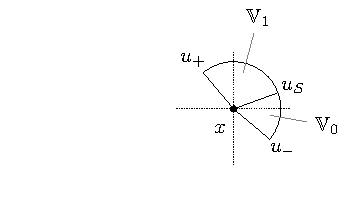
\includegraphics{clockCase1.pdf}
\hspace*{-1.5cm} 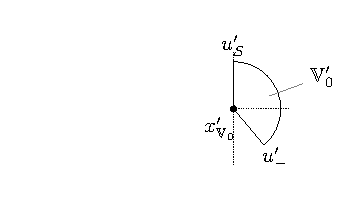
\includegraphics{clockCase1b.pdf}
\hspace*{-2.5cm} 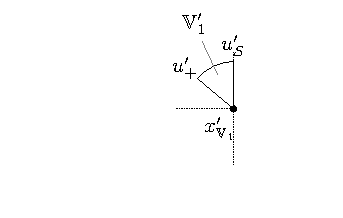
\includegraphics{clockCase1a.pdf}\\
\hspace*{-2.5cm} 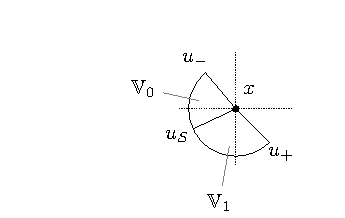
\includegraphics{clockCase2.pdf}
\hspace*{-1.5cm} 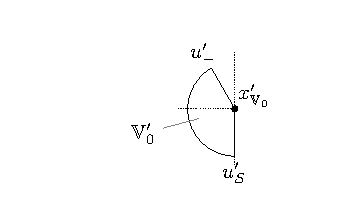
\includegraphics{clockCase2b.pdf}
\hspace*{-4.5cm} 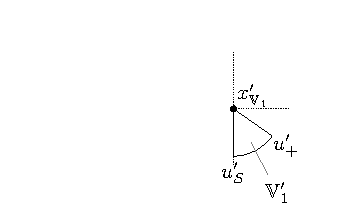
\includegraphics{clockCase2a.pdf}\\
\hspace*{-2.5cm} 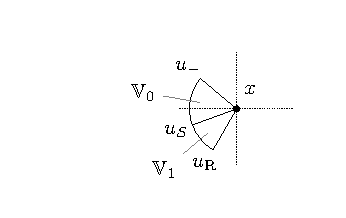
\includegraphics{clockCase3.pdf}
\hspace*{-1.5cm} 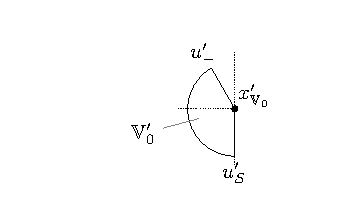
\includegraphics{clockCase3b.pdf}
\hspace*{-4.5cm} 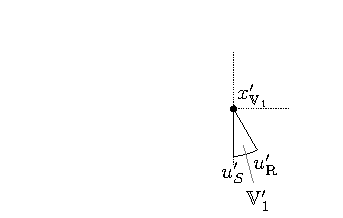
\includegraphics{clockCase3a.pdf}\\
\caption{The three possible cutting cases for $\cV$ by $\sing{1}$ in regular sectors (on the left), and their images (on the right) by the two induced maps $\cm_{\cV_{0}*}$ and $\cm_{\cV_{1}*}$\ respectively.}\label{f_cases}
\end{figure} In case (b), we necessarily have that $x\in\singForward\indCell$. We subdivide the argument into two further subcases: (i) $x\nin\singReco^{+}$; (ii) $x\in\singReco^{+}.$

In case (i), $\singForward{\indCell}$ cuts $\cV$ in exactly two sectors, induced by $\cell^{+}_{\indCell}$ and $\cell^{+}_{\indCell+1}$. Notice that these two sectors have a common boundary vector, which is induced by $\singForward{\indCell}$: we can then write the two sectors as $\cV_0 = \cV(u_-,u_\sing{})$ and $\cV_1 = \cV(u_{\sing{}},u_+)$ (see Figure~\ref{f_cases}, first and second row). We say we are in case $i'$ if $\cV$ contains the first quadrant (see first row of Figure~\ref{f_cases}) and in case $i''$ if $\cV$ contains the third quadrant (see second row of Figure~\ref{f_cases}).

Consider first case $i'$. By inspection we gather that $\cV_0$ is induced by $\cell^{+}_{\indCell+1}$ and $\cV_1$ is induced by $\cell^{+}_{\indCell}.$ Since we assume both sectors to be regular, Lemma~\ref{l_singularityStructure}$\MK$\eqref{i_adjacentCells} implies that
\begin{align*}
\lim_{y\to x}\cm_{\cV_{0}} x&\in\{0\}\times\reals^+, &
\lim_{y\to x}\cm_{\cV_{1}} x&\in\{1\}\times\reals^+.
\end{align*}
Thus the image $\cm_{\cV_0*}u_{\sing{}}$ (resp. $\cm_{\cV_1*}u_{\sing{}}$) is a vertical vector. Moreover, since $u_{\sing{}}$ lies in the first quadrant, then both its images are vertical vectors pointing upwards. The other boundary vector of each $\cV_{i}$ is one of the original vectors $u_{\pm}$, and thus its image is unstable. Since $\cm_{\cV_i*}$ is orientation preserving, we conclude that only one of the images of $\cV_i$'s can be an active sector (see again Figure~\ref{f_cases}, row 1).

Case $i''$ is completely analogous. In this case $\cV_0$ is induced by $\cell^{+}_{\indCell}$ and $\cV_1$ is induced by $\cell^{+}_{\indCell+1}$. Once again, since both sectors are regular, we gather by Lemma~\ref{l_singularityStructure}$\MK$\eqref{i_adjacentCells} that
\begin{align*}
\lim_{y\to x}\cm_{\cV_{0}} x&\in\{1\}\times\reals^+,&
\lim_{y\to x}\cm_{\cV_{1}} x&\in\{0\}\times\reals^+.
\end{align*}
Hence the image $ \cm_{x,\cV_0*} u_{\sing{}}$ (resp. $D\cm_{x,\cV_1*} u_{\sing{}}$) is a vertical vector. Moreover, since $u_{\sing{}}$ lies in the third quadrant, then both its images are vertical vectors pointing downwards. The other boundary vector of each $\cV_{i}$ is one of the original vectors $u_{\pm}$, and thus its image is unstable. Since $\cm_{\cV_i*}$ is orientation preserving, we conclude that only one of the images of $\cV_i$'s can be an active sector (see Figure~\ref{f_cases}, second row). This completes the proof in case (i).

In case (ii), combining Lemma~\ref{LmSingF} (we need the part concerning $\singForward{}$!) with Lemma~\ref{l_forwardReco} we gather that $x$ is the right endpoint of $\singForward\indCell$. Therefore $\singForward\indCell$ will cut $\cV$ only if $\cV$ contains the third quadrant. Thus, if $\cV$ contains the first quadrant, then $\singForward\indCell$ does not cut $\cV$. Hence $\cV$ could only be cut by $\singReco^+$. By the earlier discussion in this case $\cV$, contains at most one regular sector, concluding the proof in this case.

It remains to consider the more difficult case in which $\cV$ contains the third quadrant (Figure~\ref{f_cases}, bottom row). Since $x$ is the right endpoint of $\singForward{\indCell}$, we conclude that the vector induced by $\singForward{\indCell}$ must meet with $\singReco^{+}$ on the left. Therefore the two regular sectors are $\cV_0 = \cV(u_-,u_\sing{})$ and $\cV_1 = \cV(u_{\sing{}},u_{\recoPrivate})$. As in case $i'',$ we have that $\cV_0$ is induced by $\cell^{+}_{\indCell}$ and $\cV_1$ is induced by $\cell^{+}_{\indCell+1}$; the vector $u_{\recoPrivate}$ is induced by $\singReco^{+}$. Following the same reasoning as in case $i''$ above, we conclude that the image $\cm_{\cV_0*}u_{\sing{}}$ (resp. $\cm_{\cV_1*}u_{\sing{}}$) is a vertical vector pointing downwards. The image $\cm_{\cV_0*}u_{-}$ is of course unstable and belongs to the second quadrant. The image of $u_{\recoPrivate}$ is also in $\conen$ (as it will be induced by some curve in $\sing{-1}$) and points downwards. Hence, only $\cV_0'$ is active.

This concludes the argument in case (ii) and finishes the proof.
\end{proof}
\section{Invariant manifolds.}\label{sec:invariant-manifolds}
The expansion estimate proved in the previous section is the main ingredient for the so-called Growth Lemma (Lemma~\ref{l_growth}). In turn the Growth Lemma constitutes the backbone for proving ergodicity using the Hopf argument, as will be done in the next section. The Hopf argument relies on existence of a large set of points having sufficiently long stable and unstable manifolds. The present section contains necessary results about the existence of stable and unstable manifolds as well as regularity of partition of the phase space into stable and unstable manifolds. In this section we always assume that the Fermi--Ulam model is regular at infinity.

As a notational convention, in this section we drop the superscripts from $\dadm{W}(\cdot,\cdot)$, as they can be unambiguously recovered from the context.


\subsection{The Growth Lemma}\label{sec:growth-lemma}
In this section we state and prove a version of the Growth Lemma for our system. This lemma allows us to obtain, in the next subsection, a good lower bound on the length of stable and unstable manifolds passing through most of the points.

Let $W$ be an unstable curve and $x\in W$. We define $r_W(x)$ as the $\admName$-length of the shortest of the two subcurves $x$ subdivides $W$ into. The function $r_{W}(x)$ measures, in an appropriate way, the distance of $x$ to the boundary of $W$. Observe that if $W$ is weakly homogeneous, we have, by~\eqref{eq:dW-over-d-bound},\; $r_{W}(x) < \const \dadm(x,\hhs)$.

Observe moreover that
\begin{align}\label{eq:trivial-bound-for-r}
\Leb_{W}(r_{W}(x) < \eps) = \min\{2\eps,\Leb_{W}(W)\}
\end{align}
(recall that $\Leb_{W}$ denotes Lebesgue measure on the curve $W$ with respect to the $\admName$-metric).

Given an unstable curve $W,$ a point $x\in W$ and $n\ge 0$, we define $W_{n}(x)$ as follows. If $x\in\hsing n$ we let $W_{n}(x) = \emptyset$; otherwise we let $W_{n}(x)$ to be the H-component of $\cm^{n} W$ that contains $\cm^{n} x$ (recall the discussion before Proposition~\ref{p_expansionEstimate}). Then we define $r_{W,n}(x) = r_{W_{n}(x)}(\cm^{n}x)$ (or $0$ if $W_{n}(x) = \emptyset$).

Likewise, given an unstable curve $W$, $x\in W$ and $n\ge 0$, we define $\widehat{W}_{n}(x)$ and $\hat r_{W,n}$ as follows. Recall the definition of $\Np_{n}$ given before Remark~\ref{remark:definition-Npk}. If $\Np_{n}(x)$ is not defined, we let $\widehat{W}_{n}(x) = \emptyset$ and $\hat r_{W,n}(x) = 0$. Otherwise we let $\widehat{W}_{n}(x) = W_{\Np_{n}(x)}(x)$ and $\hat r_{W,n}(x) = r_{W,\Np_{n}(x)}(x)$.


\begin{lemm}
We have $r_{W,0} = \hat r_{W,0} = r_{W}$ and
\begin{align}\label{eq:silly-bound-on-r}
r_{W,n}(x) < \const \dadm(\cm^{n}x,\hhs).
\end{align}
Moreover, there exists $C > 1$, so that if $\cm^{n}W$ is a single H-component, then for any $x\in W$:
\begin{align}\label{eq:r-trivial-bound-connected}
r_{W,n}(x) > C\inv\Lambda^{\hat n(\cm^{n}W)} r_{W}(x),
\end{align}
where $\Lambda$ is the constant appearing in~\eqref{e_uniformHyperbolicity} and $\hat n$ was defined in~\eqref{eq:definition-hatn}.
\end{lemm}
\begin{proof}
The first two items follow immediately from the definition and our previous observation. We thus need to prove~\eqref{eq:r-trivial-bound-connected}. By definition $r_{W,n}(x) = |W'_{n}(x)|\adm$, where $W'_{n}(x)$ is shortest subcurve of $W_{n}(x)$ joining $\cm^{n}x$ with $\partial W_{n}(x)$. Since $\cm^{n}W$ is a single H-component, we conclude that $W_{n}(x) = \cm^{n}W$. Thus $W'_{n}(x)$ connects $x_{n}$ with $\partial \cm^{n}W$, and $\cm^{-n}W'_{n}(x)$ connects $x$ with $\partial W$. In particular $|\cm^{-n}W'_{n}(x)|\adm\ge r_{W}(x)$. Then the proof follows from~\eqref{e_adm-dominate}, \eqref{e_uniformHyperbolicity} and the definition of $\hat n$.
\end{proof}

The following is the classical Growth Lemma.
\begin{lemm}[Growth Lemma for $\hat r$]\label{l_growth}
Suppose that the Fermi--Ulam model is regular at infinity. Then there exist $0 < \theta<1$ and $C > 0$ so that for any sufficiently short mature \admiss{} unstable curve~$W\subset\csp$, any $\eps > 0$ and any $n > 0$
\begin{align}\label{eq:growth-lemma-induced}
\Leb_W(\hat r_{W,n}(x) < \eps)\le C\eps\,\Leb_W(W)+ C
\Leb_W\left(r_W(x)\leq \theta^{n}\eps\right).
\end{align}
\end{lemm}
\begin{proof}
The proof of the Growth Lemma follows via relatively standard arguments (see~\cite[\S5.9 and \S5.10]{ChM}) from the expansion estimate (Proposition~\ref{p_expansionEstimate}) and the distortion bounds proved in Corollary~\ref{cor:distortion}.

Recall the definition of $\hat\cL_{n}$ given right before Proposition~\ref{p_expansionEstimate}, and let $\bar n$ be the number appearing in Proposition~\ref{p_expansionEstimate}. We fix $\delta \in(0,1)$ to be sufficiently small so that
\begin{equation}\label{DefBrTheta}
\bar\theta = e^{2\Cdist\delta^{1/12}}\hat\cL_{\bar n} < 1
\end{equation}
(where $\Cdist$ is the constant appearing in Corollary~\ref{cor:distortion}) and so that $\delta$ is smaller than the $\delta$ obtained by Lemma~\ref{l_globalExpansion}$\MK$\eqref{lemm4.25.4} with $\delta_{*} = 1$ and $k = \bar n$.

Let us first assume that $W\subset \cspi$ and that $|W|\adm < \delta$. Then we claim that there exists $\bar C > 0$ so that for any $\eps > 0$:
\begin{align}\label{eq:growth-lemma-inductive-step}
\Leb_{W}(\hat r_{W,\bar n}(x) < \eps) < \bar C\eps\Leb W + \Leb_{W}\left(r_{W}(x) < e^{-\Cdist\delta^{1/12}}\bar\theta\eps\right).
\end{align}
As we observed in Corollary~\ref{cor:distortion}, our distortion bounds on unstable curves depend on their length. In this proof we will need very fine distortion bounds, and it will then be necessary to work only with sufficiently short unstable curves. This entails a partitioning for H-components that we now proceed to describe. Let $\{W_{i}\}$ denote the set of H-components of $\cmp^{\bar n}W$. We partition each $W_{i}$ into a number
\begin{align*}
k_i = \left\lfloor \frac{|W_{i}|\adm}{\delta}\right\rfloor+1
\end{align*}
of subcurves of equal $\admName$-length so that each subcurve has $\admName$-length between $\delta/2$ and~$\delta$. We denote the resulting subcurves $W_{ij}$. Observe that if $|W_{i}|\adm < \delta$, $k_{i} = 1$, and no shortening takes place. We call such subcurves
\emph{shortened H-components of $\cmp^{\bar n}W$}. We will shorten the H-components inductively every $\bar n$ steps of the induced map $\cmp$. By our choice of $\delta$, this guarantees that at each intermediate step, no H-component will have $\admName$-length exceeding $1$. Given $x\in W$, we will then denote by $\hat W'_{n}(x)$ the shortened H-component of $\cmp^{n}W$ whose interior contains $\cmp^{n}x$ (or $\emptyset$ if some image of $x$ lies on an endpoint of a shortened subcurve). We then define $\hat r'_{W,n}(x) = r_{\hat W'_{n}(x)}(\cmp^{n}x)$. Observe that $\hat r'_{W,\bar n} < \hat r_{W,\bar n}$, so that proving~\eqref{eq:growth-lemma-inductive-step} for $\hat r'_{W,n}$ will imply~\eqref{eq:growth-lemma-inductive-step} for $\hat r_{W,n}$. Let $B_{ij}\subset W_{ij}$ be the $\eps$-neighborhood (in the $\admName$-metric) of the boundary of each $W_{ij}$; in particular $\Leb_{W_{ij}}(B_{ij}) \leq 2\eps$. Then
\begin{align*}
\Leb_{W}\left(\hat r'_{W,\bar n}(x) < \eps\right) = \sum_{ij}\Leb_{W}\left(\cmp^{-\bar n}B_{ij}\right).
\end{align*}
By the distortion estimates of Corollary~\ref{cor:distortion}
\begin{align*}
\sum_{ij}\Leb_{W}\left(\cmp^{-\bar n}B_{ij}\right) &\le e^{\Cdist\delta^{1/12}}\sum_{ij}\Leb_{W}\left(\cmp^{-\bar n}W_{ij}\right)
\frac {\Leb_{W_{ij}}(B_{ij})}{\Leb_{W_{ij}}(W_{ij})}\\
& \le 2e^{\Cdist\delta^{1/12}}\eps \sum_{ij} k_{i}\frac{\Leb_{W}\left(\cmp^{-\bar n}W_{ij}\right)}{\Leb_{W_{i}}(W_{i})}.
\end{align*}

Split the above sum as $I+\RmII$ where $I$ stands for the sum over the components where the artificial subdivision was applied and $\RmII$ stands for the sum over the short components where no artificial subdivision is needed. Note that the sum in $I$ is over components satisfying $\Leb_{W_i}(W_i)\geq \delta$ and so
\begin{align*}
I\leq 2\delta\inv e^{\Cdist\delta^{1/12}}\eps
\sum_{ij}\Leb_{W}\left(\cmp^{-\bar n}W_{ij}\right) \le \bar C\eps\Leb_{W}(W)
\end{align*}
where we defined $\bar C = 2\delta\inv e^{\Cdist\delta^{1/12}}$. On the other hand in $\RmII$ there is no subdivision so $W_{ij}=W_i$. Therefore
\begin{align*}
\RmII\le 2e^{\Cdist\delta^{1/12}}\eps\sum_{i}\frac{\Leb_{W}\left(\cmp^{-\bar n}W_{ij}\right)}{\Leb_{W_{i}}(W_{i})} \le 2e^{\Cdist\delta^{1/12}}\eps\hat\cL_{\bar n}.
\end{align*}
Using~\eqref{eq:trivial-bound-for-r} and our definition~\eqref{DefBrTheta} of $\bar\theta$, we conclude that
\begin{align}\label{eq:growth-lemma-inductive-step-r'}
\Leb_{W}\left(\hat r'_{W,\bar n}(x) < \eps\right) < \bar C\eps\Leb W + \Leb_{W}\left(r_{W}(x) < e^{-\Cdist\delta^{1/12}}\bar\theta\eps\right),
\end{align}
which, as noted earlier, implies~\eqref{eq:growth-lemma-inductive-step}.

We now proceed to show that for any $k > 0$:
\begin{multline}\label{eq:growth-lemma-induced-estimate}
\Leb_{W}\left(\hat r'_{W,k\bar n}(x) < \eps\right) \\
\le e^{\Cdist\delta^{1/12}}\frac{1-\bar\theta^{k}}{1-\bar\theta}\cdot
\bar C\eps\Leb_{W}(W)+ \Leb_{W}\left(r_{W}(x) \le\bar \theta^{k}\eps\right).
\end{multline}
For $k = 1$~\eqref{eq:growth-lemma-induced-estimate} follows from~\eqref{eq:growth-lemma-inductive-step-r'}. Let us assume by induction that~\eqref{eq:growth-lemma-induced-estimate} holds for $k$ and prove it for $k+1$. Let $W' $ be a shortened H-component of $\cmp^{k\bar n} W$. By construction $W'\subset\cspi$ and $|W'|\adm < \delta$. Applying~\eqref{eq:growth-lemma-inductive-step} to $W'$ we gather:
\begin{align*}
\Leb_{W'}\left(\hat r'_{W',\bar n}(y) < \eps\right) &\le \bar C\eps\Leb_{W'}(W') +
\Leb_{W'}\left(\hat r_{W'}(y)\le e^{-\Cdist\delta^{1/12}}\bar\theta\eps\right).
\end{align*}
Let $W'' = \cmp^{-k\bar n} W'$, then by Corollary~\ref{cor:distortion}, we conclude that:
\begin{multline*}
\Leb_{W''}\left(\hat r'_{W'',(k+1)\bar n}(x) < \eps\right) \\
\le e^{\Cdist\delta^{1/12}}\bar C\eps\Leb_{W''}(W'')
 + e^{\Cdist\delta^{1/12}}\Leb_{W''} \left(\hat r'_{W'',k\bar n}(x) < e^{-\Cdist\delta^{1/12}}\bar \theta\eps\right).
\end{multline*}
Summing over all $W''$'s and applying the inductive hypothesis yields:
\begin{multline*}
\Leb_{W}(\hat r'_{W,(k+1)\bar n}(x) < \eps) 
\\
\begin{aligned}
&\le e^{\Cdist\delta^{1/12}}\bar C\eps\Leb_{W}(W)+
e^{\Cdist\delta^{1/12}}\Leb_{W}
\left(\hat r'_{W,k\bar n}(x) < e^{-\Cdist\delta^{1/12}}\bar\theta\eps\right) 
\\
&\le
e^{\Cdist\delta^{1/12}}\bar C\frac{1-\bar\theta^{k+1}}{1-\bar\theta}\eps\Leb_{W}(W)+
e^{\Cdist\delta^{1/12}}\Leb_{W} \left(r_{W}(x) < e^{-\Cdist\delta^{1/12}}\bar\theta^{k+1}\eps\right),
\end{aligned}
\end{multline*}
which proves~\eqref{eq:growth-lemma-induced-estimate} for $k+1$. Hence we can write:
\begin{align}\label{eq:growth-lemma-final-estimate}
\Leb_{W}\left(\hat r'_{W,k\bar n}(x) < \eps\right)\le C\eps\Leb_{W}(W)+\Leb_{W}(r_{W}(x) \le \bar\theta^{k}\eps).
\end{align}
where $C = \ifrac{\bar C e^{\Cdist\delta^{1/12}}}{(1-\theta)}$.

We now extend this estimate to iterates that are not multiples of $\bar n$. We begin by obtaining a bound on $\Leb_{W}(\hat r'_{W,s}(x) < \eps)$ for $s < \bar n$. Notice that no partitioning into short curves occurs before step $\bar n$, therefore if $\{W_{i}\}$ denotes the set of $H$-components of $\cmp^{s}W$, we have
\begin{align*}
\Leb_{W}(\hat r'_{W,s}(x) < \eps) = \Leb_{W}(\hat r_{W,s}(x) < \eps) = \sum_{i}\Leb_{W}(\cmp^{-s}B_{i}),
\end{align*}
where $B_{i}$ is a $\eps$-neighborhood of the boundary of $W_{i}$. Then we proceed as before. Since $|W|\adm < \delta$, we are guaranteed that $|W'|\adm < 1$. Thus, applying the distortion bounds in Corollary~\ref{cor:distortion}, we gather:
\begin{align*}
\sum_{i}\Leb_{W}(\cmp^{-s}B_{i})&\le 2e^{\Cdist}\eps \sum_{i}\frac{\Leb_{W}(\cmp^{-s}W_{i})}{\Leb_{W_{i}}(W_{i})}\le 2 e^{\Cdist}\eps\hat\cL_{s}.
\end{align*}
Applying once again~\eqref{eq:trivial-bound-for-r}, and observing that $\hat\cL_{s}$ is bounded uniformly in $s$, by Proposition~\ref{p_expansionEstimate}, yields:
\begin{align}\label{eq:growth-lemma-transient-bound}
\Leb_{W}(\hat r_{W,s}(x) < \eps)\le \Leb_{W}(r_{W}(x) < \Const\eps).
\end{align}
Now, for any $m > 0$, we write $m = k\bar n+s$, with $0 \le s < \bar n$. Applying~\eqref{eq:growth-lemma-transient-bound} to each shortened component $W'$ of $\cmp^{k\bar n}W$ yields:
\begin{align*}
\Leb_{W'}\left(\hat r_{W',s}(y) < \eps\right)\le \Leb_{W'}(r_{W '}(x) < \Const\eps).
\end{align*}
Taking $W'' = \cmp^{-k\bar n}W'\subset W$, and applying the distortion bounds:
\begin{align*}
\Leb_{W''}\left(\hat r_{W'',k\bar n+s}(x) < \eps\right)&
\le e^{\Cdist\delta^{1/12}}\Leb_{W''}\left(r'_{W'',k\bar n}(x) < \Const\eps\right).
\end{align*}
Now summing over all $W''$ and applying~\eqref{eq:growth-lemma-final-estimate}, we finally conclude that
\begin{align*}
\Leb_{W}(\hat r_{W,k\bar n+s}(x) < \eps)&
\le e^{\Cdist\delta^{1/12}}C\eps\Leb_{W}(W)+\Leb_{W}\left(r_{W}(x)\le \Const\bar \theta^{k}\eps\right).
\end{align*}
Choosing $\theta = \bar\theta^{1/\bar n}$ and $C = \Const\theta\inv$ yields~\eqref{eq:growth-lemma-induced} under the assumption $W\subset \cspi$ and $|W|\adm < \delta$.

Now, observe that, given an unstable curve $W$, for any $x\in W$, $\hat W_{1}(x)$ is either $\emptyset$ or it is a curve $W'\subset\cspi$. By Lemma~\ref{l_globalExpansion}$\MK$\eqref{lemm4.25.4} it is possible to assume that $W$ is so short that each $W'$ is such that $|W'|\adm < \delta$. By applying once again the distortion argument, we deduce that~\eqref{eq:growth-lemma-induced} holds in the general case, by suitably increasing the constants.
\end{proof}

We are now going to complement the Growth Lemma above (which involves iterates of $W$ by $\cmp$) with some estimates on the length of the iterates of unstable curves by~$\cm$. More precisely, let $W$ be an unstable curve and $x\in W$. Define
\begin{align*}
\bar r_{W}(x) = \min_{0\,\le\,n\,<\,\Np(x)}r_{W,n}(x),
\end{align*}
with the convention that if $\Np(x)$ is undefined, then $\bar r_{W}(x) = 0$.

\begin{lemm}[Transient growth control]\label{lem:transient-growth-control}
There is $C > 0$ so that for any sufficiently short mature
\admiss{} unstable curve $W$ and any $\eps<\delta$
\begin{align*}
\Leb_{W}(\bar r_{W}(x) < \eps) < \Leb_{W}(r_{W}(x) < C\eps).
\end{align*}
\end{lemm}
\begin{proof}
The proof follows from distortion arguments similar to the ones given in the proof of the Growth Lemma. Assume that $|W|\adm < \delta$.

Recall that the constant $\law4$ was introduced in Lemma~\ref{l_largeCell}$\MK$\eqref{i_almostFinite-large}. Assume first that $W\cap\cspiu{\law4}\ne\emptyset$. Then there exists $N_{*} = \Const \law4$ so that $\Np(x) < N_{*}$ for any $x\in W$. Thus:
\begin{align*}
\Leb_{W}(\bar r_{W}(x) < \eps) &\le \sum_{n = 0}^{N_{*}-1}\Leb_{W}(r_{W,n}(x) < \eps).
\end{align*}
We proceed to obtain a bound on $\Leb_{W}(r_{W,n}(x) < \eps)$. Let us fix $n > 0$ and let $\{W_{i}\}$ denote the set of H-components of $\cm^{n}W$; let $B_{i}\subset W_i$ be the $\eps$-neighborhood of the boundary of $W_{i}$. Then
\begin{align*}
\Leb_{W}(r_{W,n}(x) < \eps) = \sum_{i}\Leb_{W}(\cm^{-n}B_{i}).
\end{align*}
Assuming $|W|\adm < \delta$, we are guaranteed that each component $W_{i}$ satisfies $|W_{i}|\adm < 1$. Hence by our distortion bounds (Corollary~\ref{cor:distortion})
\begin{align*}
\sum_{i}\Leb_{W}(\cm^{-n}B_{i})\le 2e^{\Cdist}\eps
\sum_{i}\frac{\Leb_{W}(\cm^{-n}W_{i})}{\Leb_{W}(W_{i})}
\end{align*}
\begin{align*}
\le 2e^{\Cdist}\eps \cL_{n}(W)
\le \Leb_{W}\left(r_{W}(x) < e^{\Cdist}\cL_{n}\eps\right).
\end{align*}
%{eq:cL-submultiplicative}
By~\eqref{eq:cL-submultiplicative}, $\cL_{n}\le\cL_{1}^{n}.$ Thus $\cL_{n}\le\max\{1,\cL_{1}^{N_{*}}\}$, which is bounded by~\eqref{eq:cl1-bounded}. This concludes the proof of the lemma in the case of low energies.

Next, consider the case $W\subset\cspil{\law4}\ne\emptyset$. Then if $\delta$ sufficiently small, by Lem\-ma~\ref{l_largeCell}$\MK$\eqref{i_almostFinite-large}, $W$ intersects at most two cells $\cEs_{n}$. Such cells partition $W$ in (at most) two subcurves $W_{1}$ and $W_{2}$ so that $\Np(x) = N_{*}$ for all $x\in W_{1}$ and $\Np(x) = N_{*}+1$ for all $x\in W_{2}$, for some $N_{*} > 0$. Note that
\begin{align*}
\Leb_{W}(\bar r_{W}(x) < \eps)\le\Leb_{W}(\bar r_{W_{1}}(x) < \eps) + \Leb_{W}(\bar r_{W_{2}}(x) < \eps).
\end{align*}

Consider $\bar r_{W_{1}}(x)$. By construction $W_{1}\subset\cEs_{N_{*}}$. Since $\cEs_{N_{*}}\cap\sing{N_{*}-1} = \emptyset$, we gather that $\cm^{n}W_{1}$ is connected for any $0\le n < N_{*}$. Thus, \eqref{eq:r-trivial-bound-connected} ensures that $r_{W_{1},n}(x)\ge C\inv r_{W_{1}}(x)$ for any $n < N_{*}$, and therefore $\bar r_{W_{1}}(x) \ge C\inv r_{W_{1}}(x)$. By the same token $\bar r_{W_{2}}(x) \ge C\inv r_{W_{2}}(x)$. Hence
\begin{align*}
\Leb_{W}(\bar r_{W}(x) < \eps) \le \Leb_{W}(r_{W} < 2C\eps)
\end{align*}
which concludes the proof of the Lemma~\ref{lem:transient-growth-control}.
\end{proof}

In order to obtain bounds on the length of stable and unstable manifolds, we will need some results similar to the ones presented above, but for slightly different functions $r$. We now proceed to define them and link their properties to the ones of the functions $r$ that have been investigated above.

Recall the properties of the singularity sets $\singBoth$ outlined in Lemma~\ref{LmSingF} and define, for $N \ge 0$:
\begin{align*}
\singForward{(N)} &= \sing{0}\cup\singForward\recoPrivate\cup\bigcup_{\indCell = 0}^{N}\singForward{\indCell}.
\end{align*}
For $x\in W$ let us define $r_W(x,\singForward{(N)})$ as follows. If $x\in\singForward{(N)}$ we set $r_W(x,\singForward{(N)}) = 0$. Otherwise $\singForward{(N)}$ cuts $W$ into finitely many subcurves. Let $W'$ be the subcurve that contains $x$ and $r_W(x,\singForward{(N)}) = r_{W'}(x)$. Observe that necessarily $r_{W}(x,\singForward{(N)})\le r_{W}(x)$. Finally define\footnote{ The motivation for this definition will become clear to the reader in the proof of Lemma~\ref{lem:kolya-patch}.}
\begin{align*}
r_{W}^{*}(x) = \inf_{N > 0}\left\{N^{3/2}r_{W}\left(x,\singForward{(N)}\right)\right\}.
\end{align*}

Notice that $r^{*}_{W}(x)\le r_{W}(x)$, and it could, in principle, be much smaller than $r_{W}$. However, the measure of points where this possibility occurs is under control thanks to the following bound.


\begin{lemm}\label{lem:r-star-vs-r}
There exists $C > 0$ so that for any unstable curve $W$ and any $0 < \eps<\delta$
\begin{align*}
\Leb_{W}(r^{*}_{W}(x) < \eps)\le \Leb_W(r_{W}(x) < C\eps).
\end{align*}
\end{lemm}
\begin{proof}
By Lemma~\ref{LmSingF}, we conclude that the set $\{r_{W}^{*}(x) < \eps\}$ is contained in the union of
\begin{itemize}
\item 2 intervals of $\admName$-length $\eps$ at the boundary of $W$;

\item an interval of $\admName$-length $2\eps$ centered at each point of $W\cap(\singForward{\recoPrivate}\cup\singForward{0})$;

\item an interval of $\admName$-length $2\indCell^{-3/2}\eps$ centered at each point of $W\cap\singForward{\indCell}$ for $\nu>0$.
\end{itemize}

Hence
\begin{align*}
\Leb_{W}(r_{W}^{*}(x) < \eps) < 2\eps \left(1+2+\sum_{\indCell\,>\,0}\indCell^{-3/2}\right) < 2\Const\eps.
\end{align*}
Since $\Leb_{W}(r_{W}(x) < C\eps)\leq 2 C \eps$ we conclude that
\begin{align*}
\Leb_{W}(r_{W}^{*}(x) < \eps) & \le \Leb_{W}(r_{W}(x) < C\eps).\qedhere
\end{align*}
\end{proof}

Using the above lemma, it is possible to obtain a Growth Lemma and transient growth control for $r^{*}$. Let $W$ be an unstable curve and $x\in W$. For $n\ge0$ we define $r^{*}_{W,n}(x)$ as follows: if $x\in\hsing n$ we let $r^{*}_{W,n}(x) = 0$; otherwise $W_{n}(x)\ne\emptyset$ and we set
\begin{align*}
r^{*}_{W,n}(x) = r^{*}_{W_{n}(x)}(\cm^{n}x).
\end{align*}
Likewise, given $n\ge 0$, if $\Np_{n}(x)$ is not defined, we let $\hat r^{*}_{W,n}(x) = 0$. Otherwise we define
\begin{equation}\label{DefHatR}
\hat r^{*}_{W,n}(x) = r^{*}_{W,\Np_{n}(x)}(x).
\end{equation}
Finally, let $x\in W$. If $\Np(x)$ is undefined, set $\bar r^{*}_{W}(x) = 0$. Otherwise let
\begin{align*}
\bar r^{*}_{W}(x) &= \min_{0\,\le\,n\,<\,\Np(x)}r^{*}_{W,n}(x).
\end{align*}
We now prove for $\bar r^{*}$ the bounds of Lemma~\ref{lem:transient-growth-control}.

\begin{lemm}\label{lem:transient-growth-control-star}
There exists $C > 0$ so that for any sufficiently short mature
\admiss{} unstable curve $W\subset \csp$ and any $0 < \eps<\delta$ we have:
\begin{align}\label{eq:transient-growth-r-star}
\Leb_{W}\left(\bar r^{*}_{W}(x) < \eps\right) &< \Leb_{W}(r_{W}(x) < C\eps).
\end{align}
\end{lemm}

\begin{proof}
Assume $|W|\adm < \delta$; let $\lawc$ be sufficiently large and consider first the case where $W\cap\cspl{\lawc}\ne\emptyset$. Then if $\delta\leq 1$, Proposition~\ref{p_largeEnergiesFUM}\ref{i_boundOnExcursion} implies that for any $x\in W$ and any $0\le n < \Np(x)$, $\cm^{n}x\in\cspl{\lawc/C}$. Notice that Lemma~\ref{LmSingF} and the construction of $\cEs_{n}$ guarantees that $\cEs_{n}\cap\sing+ = \emptyset$ unless $n = 1$. By Lemma~\ref{LmSingF}$\MK$\eqref{lemm3.11.4} $\sing+_{\indCell}$ is compact for $\indCell > 0$. Therefore for large enough $\lawc$, the only possible curve of $\sing+$ that intersects with $\cEs_{1}\cap\cspl{\lawc/C}$ is $\sing+_{0}$, but $\sing+_{0}\subset\partial\cEs_{1}$; we conclude that $\cEs_{1}\cap\cspl{\lawc/C} \cap \sing+ = \emptyset$. We thus proceed as in the proof of Lemma~\ref{lem:transient-growth-control}. If $\lawc$ is sufficiently large and $\delta$ sufficiently small, by Lemma~\ref{l_largeCell}$\MK$\eqref{i_almostFinite-large}, $W$ intersects at most two cells $\cEs_{n}$; such cells partition $W$ in (at most) two subcurves $W_{1}$ and $W_{2}$. Then
\begin{align*}
\Leb_{W}(\bar r^{*}_{W}(x) < \eps)&\le
\Leb_{W}(\bar r^{*}_{W_{1}}(x) < \eps)+
\Leb_{W}(\bar r^{*}_{W_{2}}(x) < \eps).
\end{align*}
Notice that $\cm^{n}W_{i}$ will belong to only one cell $\cEs_{\indCell}$ for any $n$ involved in the definition of $\bar r^{*}_{W_{i}}$. By the argument above, we gather that $\bar r^{*}_{W_{i}} = \bar r_{W_{i}}$. Now we conclude arguing as in the proof of Lemma~\ref{lem:transient-growth-control}.

{ Next, consider the case} $W\subset\cspu{\lawc}$. Then there exists $N_{*} = \Const\lawc$ so that $\Np(x) < N_{*}$ for any $x\in W$. Thus:
\begin{align*}
\Leb_{W}(\bar r^{*}_{W}(x) < \eps)\le \sum_{n = 0}^{N_{*}-1}
\Leb_{W}(r^{*}_{W,n}(x) < \eps).
\end{align*}
Lemma~\ref{lem:r-star-vs-r} then implies that
\begin{align*}
\Leb_{W}(\bar r_{W}^{*}(x) < \eps)\le \sum_{n = 0}^{N_{*}-1}\Leb_{W}(r_{W,n}(x) < C\eps).
\end{align*}
Now arguing as in the proof of Lemma~\ref{lem:transient-growth-control}, we obtain~\eqref{eq:transient-growth-r-star} in the second case.
\end{proof}

\subsection{Size of invariant manifolds.}\label{SSInvMan}
Recall that an unstable curve $W$ is a homogeneous unstable manifold if $W\subset\csp\setminus\hsing{-\infty}$ (resp. a stable curve $W$ is a homogeneous stable manifold if $W\subset\csp\setminus\hsing{+\infty}$). By Lemma~\ref{lem:properties_stable_mfolds}, we have $|\cm^{-n}W|\adm\to 0$ as $n\to\infty$ (resp. $|\cm^{n}W|\adm\to 0$ as $n\to\infty$). Given $x\in \csp$, we denote by $\Wu(x)$ (resp. $\Ws(x)$) the \emph{maximal} homogeneous unstable (resp. stable) manifold containing $x$ (or $\emptyset$ if such manifold does not exist). Conventionally, we consider such curves without the endpoints.

We now give a convenient characterization of $\Ws(x)$ and $\Wu(x)$. The construction closely follows~\cite[\S4.11]{ChM}, and we refer the reader to that section for additional properties. For $x\in\csp\setminus\hsing{-\infty}$, and $n > 0$, we denote by $Q^{\homo}_{-n}(x)$ the connected component of the open set $\csp\setminus\hsing{-n}$ that contains $x$. Naturally, $Q^{\homo}_{-n}(x)\supset Q^{\homo}_{-(n+1)}(x)$ for any $n$. Moreover $\overline{Q^{\homo}_{-n}(x)}$ is compact for any $n$ sufficiently large, possibly depending on $x$.\footnote{Compactness holds since, for $n$ sufficiently large (e.g. $n > \Np(x)+\Np(\cm^{\Np(x)}(x))$), the set $\cm^{\Np(x)}Q_n(x)$ is contained in some fundamental domain $\Dom_{m}$, and such sets are bounded (see e.g.~\eqref{Per-W}).} An analogous construction yields the definition of $Q^{\homo}_{n}(x)$ for $n > 0$. To simplify our exposition, we drop the superscript $\homo$ from $Q^{\homo}$ for the remainder of this section.\footnote{This introduces a slight abuse of notation with the sets $Q_{n}$ defined in \S\ref{ss_regularComplexity}.}
%\sallskip

\begin{lemm}\label{lem:almost-density}
Let $x\in\csp\setminus\hsing{-\infty}$ and $(W_{n})_{n\,>\,0}$ be a sequence of admissible unstable curves passing through $x$ such that $W_{n} = \cm^{n}V_{n}$ where $V_{n}$ is unstable and $V_{n}\subset Q_{n}(\cm^{-n}x)$ (hence in particular $W_{n}\subset Q_{-n}(x)$). Then, there exists a subsequence $(W_{n_{k}})_{k\,>\,0}$ that converges in $C^{1}$ to a subcurve of $\Wu(x)$. Analogous statements hold for stable curves and stable manifolds.
\end{lemm}
\begin{proof}
We prove the lemma as stated; the corresponding statements for stable curves and manifolds follow by involution. First, we can assume that there exists $\eta > 0$ so that $|W_{n}|\adm > \eta$ (otherwise, the statement trivially holds by choosing a subsequence so that $|W_{n_{k}}|\adm\to 0$, which converges to $x$).

By definition of admissible curve (see the first paragraph of
\S\ref{sec:unstable-curves}), and Arzel\`a--Ascoli Theorem, we can extract a subsequence $W_{n_{k}}$ that converges in the $C^{1}$-topology to some $C^{1}$-curve $W$; as usual, $W$ denotes the limit curve without the endpoints. We now show that $W\subset \bigcap_{n\,>\,0} Q_{-n}(x)$, which will conclude the proof of the lemma, since in particular this fact implies $W\cap\hsing{-\infty} = \emptyset$. First of all, by construction, we have that $W\subset\bigcap_{n\,>\,0}\overline{Q_{-n}(x)}$: otherwise there would exist $\bar n > 0$ and infinitely many curves $W_{n}$ so that $W_{n}\not\subset Q_{-\bar n}(x)$, which contradicts our hypothesis. Assume now that there exists $x'\in W$ such that $x'\not\in \bigcap_{n\,>\,0}Q_{-n}(x)$, i.e. there exists $n^{*}$ so that $x'\in\partial Q_{-n^{*}}(x)$; in particular $x'\in\hsing{-n^{*}}$. By Remark~\ref{remark:singularity-order}, $\partial Q_{-n_{*}}(x)$ is comprised of curves compatible with $\conen\cap D\cm^{n^{*}}\conep$. On the other hand, $W$ is a limit of unstable curves $W_{n_{k}}$ that are compatible with $D\cm^{n_{k}}\coneu$; observe that near $x'$ the cone $\conen\cap D\cm^{n^{*}}\conep$ is transverse to the cone $D\cm^{n_{k}}\coneu$ if $k$ is sufficiently large (this holds by strict invariance of the unstable cones). It follows that for arbitrarily large $k$, the curve $W_{n_{k}}$ will intersect (and thus terminate on) $\partial Q_{-n^{*}}(x)$ arbitrarily close to $x'$; we conclude that $x'$ is an endpoint of $W$, which contradicts our assumption.
\end{proof}


If $\Wu(x) = \emptyset$ we define $\ru(x) = 0$. Otherwise, $x$ subdivides $\Wu(x)$ in two subcurves, we denote by $\ru(x)$ the $\admName$-length of the shortest subcurve. Define $\rs(x)$ similarly.

To obtain lower bounds for $\rs$ and $\ru$ we need to introduce some notation. Given $x\in\csp$, define the functions $E^{\pm}:\csp\to\reals$ so that if $x\in\homo_{k}\cap\cell^{\pm}_{\indCell}$, then $E^{\pm}(x) = (\indCell+1)(k^{2}+1)$. More precisely
\begin{align*}
E^{\pm}(x) &= \sum_{k}(k^{2}+1)\If_{\homo_{k}\,\cap\,\cell^{\pm}_{\recoPrivate}}+\sum_{k,\indCell}(k^{2}+1)(\indCell+1)\If_{\homo_{k}\,\cap\,\cell^{\pm}_{\indCell}}(x),
\end{align*}
where $\If_{A}$ denotes the indicator of the set $A$.

$E^{\pm}$ controls the contraction and expansion of stable and unstable vectors by $D\cm$ as follows.
\begin{lemm}
There exists a constant $C>0$ such that
\begin{subequations}\label{eq:function-E}
\begin{align}\label{FunE1}
C\inv E^{-}(\cm x) &< \frac {|D_{x}\cm u^{\unstable}|\adm}{|u^{\unstable}|\adm} < C E^{-}(\cm x)& \fa x\in\csp\setminus\singForward{}, u^{\unstable}\in\coneu_{x}\\\label{FunE2}
C\inv E^{+}(\cm\inv x) &< \frac {|D_{x}\cm\inv u^{\stable}|\adm}{|u^{\stable}|\adm} < C E^{+}(\cm\inv x)& \fa x\in\csp\setminus\singBackward{}, u^{\stable}\in\cones_{x}.
\end{align}
\end{subequations}
\end{lemm}
\begin{proof}
It suffices to show~\eqref{FunE1}, then~\eqref{FunE2} follows by involution. If $\cm x\in\reco$, then the lower bound follows\footnote{ Since $\cm x\in\reco$, then $|\cdot|\adm$ and $|\cdot|_{*}$ are uniformly equivalent.} from~\eqref{e_expansionAdm-II} and the upper bound follows from~\eqref{e_expansionAuxMetricA} and Corollary~\ref{CrHESqueeze}\ref{i_lower-bound-prpslope}. Next, suppose $\cm x = (\ct',w')\nin\reco$. If $w' > \law2$ (where $\law2$ is defined in Corollary~\ref{CrHESqueeze}), then our estimates follow\footnote{Observe that, even though in this region $|\cdot|\adm$ and $|\cdot|_{*}$ are not uniformly equivalent, we still have
\begin{align*}
\const\inv \frac{|D_{x}\cm u|\adm}{|u|\adm} < \frac{|D_{x}\cm u|_{*}}{|u|_{*}} < \const \frac{|D_{x}\cm u|\adm}{|u|\adm}\,.
\end{align*}
} from Corollary~\ref{CrHESqueeze} and~\eqref{e_expansionAuxMetricA}. If, on the other hand, $w'\le\law2$, we have $w < \law2+\Const$ and since $x\nin\cl\reco$, we obtain the estimates using Lemma~\ref{LmPSlopeC0}$\MK$\eqref{lemm4.12.2}and~\eqref{e_expansionAuxMetricA}.
\end{proof}

Given $x\in\csp$ and $n\in\bZ$, we denote with $\ds(x,\hsing n)$ (resp. $\du(x,\hsing n)$) the length (in the $\admName$-metric) of the shortest\footnote{The existence of such a curve follows from the fact that the stable (resp. unstable) cone is closed and that the singularity set is closed.} stable (resp. unstable) curve which connects $x$ with $\hsing n$.

For $x\in\csp$, let $\Lambda^{\unstable}_{n}(x)$ be the minimal expansion of unstable vectors by $D_{x}\cm^{n}$. Similarly, let $\Lambda^{\stable}_{n}(x)$ be the minimal expansion of stable vectors by $D_{x}\cm^{-n}$. Notice that there exists $\underline\Lambda > 0$ so that for any $n > 0$ and $x\in\csp$
\begin{align}\label{eq:lambda-lowerbar}
\Lambda_{n}^{\stable}(x) > \underline\Lambda, \quad
\Lambda_{n}^{\unstable}(x) > \underline\Lambda
\end{align}
(see e.g. Proposition~\ref{p_propertiesAdm}). Moreover, by definition, for any $0 < m < n$:
\begin{align*}
\Lambda^{\unstable}_{n}(x)&\ge\Lambda^{\unstable}_{m}(x)\Lambda^{\unstable}_{n-m}(\cm^{m}x)&
\Lambda^{\stable}_{n}(x)&\ge\Lambda^{\stable}_{m}(x)\Lambda^{\stable}_{n-m}(\cm^{-m}x).
\end{align*}
Hence by~\eqref{eq:function-E}, for any $n\ge 1$
\begin{subequations}
\begin{align}\label{eq:lambda-E}
\Lambda^{\unstable}_{n}(x)&\ge C^{-1} E^{-}(\cm x)\Lambda^{\unstable}_{n-1}(\cm x),\\\label{eq:lambda-EE}
\Lambda^{\stable}_{n}(x)&\ge C^{-1} E^{+}(\cm\inv x)\Lambda^{\stable}_{n-1}(\cm\inv x).
\end{align}
\end{subequations}

\begin{lemm} \label{PrSize}
For any $L > 0$ there exists a constant $c > 0$ such that
\begin{align*}
\rs(x)&\geq \min\left\{L,c \inf_{n\, >\,0} \Lambda_{n}^{\stable}\left(\cm^{n}x\right) \ds\left(\cm^{n}x, \hsing{-1}\right)\right\},\\
\ru(x)&\geq \min\left\{L,c \inf_{n\,>\,0} \Lambda_{n}^{\unstable}\left(\cm^{-n}x\right) \du\left(\cm^{-n}x, \hsing{1}\right)\right\}.
\end{align*}
\end{lemm}
\begin{proof}
The proof of the lemma is a combination of the arguments given in~\cite[Lemma~4.67, (4.61), Exercise~5.19 and (5.58)]{ChM}.

Let us prove the statement for $\ru$ (the statement for $\rs$ follows as usual by the properties of the involution). We may further assume that $x\in\csp\setminus\hsing{-\infty}$ (otherwise the right hand side of the inequality is $0$ and the statement holds trivially). As before, for any $n$, we let $Q_{-n}(x)$ be the connected component of $\csp\setminus\hsing{-n}$ containing the point $x$. Clearly $Q_n(\cm^{-n}x) = \cm^{-n}(Q_{-n}(x))$ is the connected component of $\csp\setminus\hsing{n}$ containing the point $\cm^{-n}x$. Let $n^{*}$ be so large that $\overline{Q_{-n^{*}}(x)}$ is compact. For $n > n^{*}$, $\cm^{-n}\Wu(x)\subset Q_{n}(\cm^{-n}x)$; let $V'_{n}$ be an arbitrary continuation as a mature unstable curve of $\cm^{-n}\Wu(x)$ to $\partial Q_{n}(\cm^{-n}x)$. We further assume that $V'_{n}$ is $\hat K$-\admiss{}.\footnote{By Corollary~\ref{CrUMLip}, $\cm^{-n}\Wu(x)$ is $\hat K$-\admiss{} and we can choose our continuation to satisfy this requirement} Then $W'_{n} = \cm^{n}(V'_{n})$ is an admissible unstable continuation of $\Wu(x)$ that terminates on $\partial Q_{-n}(x)$. Let us fix $\eps > 0$. By Lemma~\ref{lem:almost-density} we can choose $n$ so that the $\admName$-length of each component of $W_{n}\setminus \Wu(x)$ is smaller than $\eps$ (otherwise $\Wu(x)$ would not be maximal). $W_{n}$ is divided by the point $x$ into two subcurves; denote with $W$ the shortest one (in the $\admName$-metric). By our construction and~\eqref{e_defAdmE} we gather that $\ru(x)\ge |W|\adm- \eps$. Since $\eps$ is arbitrary, it suffices to show that
\begin{align*}
|W|\adm &\geq \min\left\{L,c \inf_{n\,>\,0} \Lambda_{n}^{\unstable}(\cm^{-n}x) \du\left(\cm^{-n}x, \hsing{1}\right)\right\}.
\end{align*}

The above bound trivially holds if $|W|\adm \ge L$. Let us thus assume that $|W|\adm < L$ and for $0\le m\le n$ let $V_{m} = \cm^{-m}W$. Since $V_{n}$ terminates on $\hsing{n}$, there exists $m\in[1,n]$ so that $V_{m}$ joins $\cm^{-m}x$ with $\hsing{1}$. We thus gather
\begin{align*}
|W|\adm= \frac{|W|\adm}{|V_{m}|\adm}|V_{m}|\adm
&\ge\Const \Lambda_{m}^{\unstable}(\cm^{-m}x) |V_{m}|\adm\\
&\ge\Const \Lambda_{m}^{\unstable}(\cm^{-m}x)\du\left(\cm^{-m}x,\hsing1\right)
\end{align*}
where we used distortion estimates obtained in Corollary~\ref{cor:distortion}.
\end{proof}

The statement we are about to prove below (Lemma~\ref{lem:kolya-patch}) is the analog of~\cite[Exercise~5.69]{ChM}, but there are some differences which are due to two separate issues. First of all the statement of that exercise is incorrect: the strategy presented in~\cite[\S5.5]{ChM} has a gap and needs to be corrected (see~\cite{kolya-patch} for a proposed solution). Second, the argument would need a non-trivial adaptation to our specific case because of the nature of our singularities (presence of corner points, non-compactness). We thus proceed to give in detail the statement and the proof of what is needed for our analysis. In order to simplify our notation we denote, as usual, $x_{n} = \cm^{n}x$.

\begin{lemm}\label{lem:kolya-patch}
There exists a constant $C > 0$ so that
\begin{subequations}
\begin{enumerate}\alphenumi
\item\label{lemm7.9.1} for any mature unstable curve $W\subset\csp$, any $n\ge 2$ and any $x\in W\setminus\sing n$:
\begin{multline}
\Lambda^{\stable}_{n}(x_{n})\ds\left(x_{n},\hsing{-1}\right)\\
 \ge C\min\left\{\Lambda^{\stable}_{n}(x_{n})r_{W,n}(x),\Lambda^{\stable}_{n-1}(x_{n-1})r^{*}_{W,n-1}(x), \Lambda^{\stable}_{n-2}(x_{n-2})r_{W,n-2}(x)\right\}.
\end{multline}
\item\label{lemm7.9.2} for any unstable curve $W\subset\csp$ that is the image of a mature unstable curve and any $x\in W\setminus\sing 1$:
\begin{align}
\Lambda^{\stable}_{1}(x_{1})\ds\left(x_{1},\hsing{-1}\right) \ge C\min\left\{ \Lambda^{\stable}_{1}(x_{1})r_{W,1}(x), r^{*}_{W}(x), r_{W}(x)^{4}\right\}.
\end{align}
\end{enumerate}
\end{subequations}
\end{lemm}
\begin{proof}
Recall that $\hsing{-1}$ is a closed set (see Remark~\ref{RkSCClosed}). In particular the distance $\ds(x_{n},\hsing{-1})$ is attained as $|V|\adm$, where $V = V(x_{n})$ is a stable curve which joins $x_{n}$ to some point $z\in\hsing{-1}$. By definition (see~\eqref{e_definitionHSing}) we have $\DS \hsing{-1} = \hhs \cup \cm(\hhs\setminus\singForward{}) \cup \singBackward{}. $ Hence there are three possibilities:
\begin{enumerate}\alphenumi
\item\label{prf7.9.a} $z\in\hhs$; 
\item\label{prf7.9.b} $z\in\cm(\hhs\setminus\singForward{})$; 
\item\label{prf7.9.c} $z\in\singBackward{}$.
\end{enumerate}

We begin with case (a). By definition it holds that $|V|\adm\ge \dadm(x_{n},\hhs)$. Using~\eqref{eq:silly-bound-on-r} we thus conclude that $\ds(x_n,\hsing{-1})\ge \const r_{W,n}(x)$.

In cases (b) and (c) we consider $V' = \cm\inv V$. Then $V'$ is a weakly homogeneous stable curve and, by~\eqref{eq:function-E}:
\begin{align*}
|V|\adm\ge \frac{\const |V'|\adm}{E^{+}(x_{n-1})}.
\end{align*}
In case (b), $V'$ links $x_{n-1}$ to some point $z'\in\hhs$, so $|V'|\adm\ge\dadm(x_{n-1},\hhs)$ and using~\eqref{eq:lambda-EE} we gather that:
\begin{align*}
\Lambda^{\stable}_{n}(x_{n})\ds(x_{n},\hsing{-1})&\ge \const\Lambda^{\stable}_{n-1}(x_{n-1})\dadm(x_{n-1},\hhs).
\end{align*}
Using again~\eqref{eq:silly-bound-on-r} we thus conclude that
\begin{align*}
\Lambda^{\stable}_{n}(x_{n})\ds\left(x_{n},\hsing{-1}\right)&\ge \const\Lambda^{\stable}_{n-1}(x_{n-1})r_{W,n-1}(x).
\end{align*}

Finally, we consider case (c). Then $V'$ is a stable curve linking $x_{n-1}$ to some\footnote{ Note that $\cm\inv$ is undefined on $\singBackward{}$ so we cannot quite say that $z' = \cm\inv z$.} point $z'\in\singForward{}$. We consider two possibilities:
\begin{enumerate}
\item[$(c')$] $x_{n-1}\in\reco$ and $z'\in\{0\}\times[0,\slopeb]$;
\item[$(c'')$] otherwise.
\end{enumerate}
In case $(c')$, observe that since $V'$ is a stable curve, it is increasing, and the assumptions in $(c')$ imply that $V'\subset\reco$ (see Lemma~\ref{l_forwardReco}). We have now to deal separately with the case $n = 1$ and $n > 1$. If $n > 1$, consider $V'' = \cm\inv V'$. Observe that $V''\subset\backReco$ is a stable (once again, increasing) curve, which joins $x_{n-2}\in\backReco$ to $z''\in\{\ct = 1\}$. The expansion of $D\cm\inv$ along $V'$ is bounded above\footnote{ Remarkably, the geometry still allows us to obtain an upper bound on expansion despite the fact that $V''$ is not, a priori, weakly homogeneous.} by $\const E^{+}(x_{n-2})$ (since $x_{n-2}\in\backReco$ and it is the lowest point on $V''$). We conclude that
\begin{align*}
|V'|\adm\ge \const \frac{|V''|\adm}{E^{+}(x_{n-2})}.
\end{align*}
Hence, $|V''|\adm\ge \dadm(x_{n-2},\{\ct = 1\})$. Now $x_{n-2}$ cuts $W_{n-2}(x)$ into two subcurves. Let $W'_{n-2}(x)$ denote the subcurve to the right of $x_{n-2}$; then by definition $|W'_{n-2}(x)|\ge r_{W,n-2}(x)$. Notice that $W'_{n-2}(x)\subset\backReco$, thus $W'_{n-2}(x)\cap\reco = \emptyset$. Corollary~\ref{CrHESqueeze} then implies that we have uniform transversality of $W'_{n-2}(x)$ with any vertical line, which allows to conclude that
\begin{align*}
\dadm{}(x_{n-2},\{\ct = 1\}) &\ge \const |W'_{n-2}(x)|\adm\ge \const r_{W,n-2}(x).
\end{align*}
Hence in case $(c')$ and if $n > 1$:
\begin{align*}
\Lambda^{\stable}_{n}(x_{n})\ds(x_{n},\hsing{-1}) &\ge \const
\Lambda^{\stable}_{n-2}(x_{n-2})r_{W,n-2}(x)\}.
\end{align*}
If $n = 1$ (which corresponds to item (b) in the statement), we need to modify the above argument as follows. Applying parts~\eqref{lemm4.25.1} and~\eqref{lemm4.25.2} of Lemma~\ref{l_globalExpansion} to the stable curve $V'\subset\reco$ (note that $|V'|$ has uniformly bounded $\admName{}$-length since $\reco$ is bounded; the same holds for $V'' = \cm\inv V'\subset\backReco$) we obtain
\begin{align*}
|V'|\adm \ge \const |V''|\adm^{2};
\end{align*}
Then arguing as before (with $W_{n-2}$ replaced by $\cm\inv W$, that is guaranteed to be a mature unstable curve by our assumption), we conclude that $|V''|\adm\ge \const r_{\cm\inv W}(x_{-1})$.

Applying once again parts~\eqref{lemm4.25.1} and~\eqref{lemm4.25.2} of Lemma~\ref{l_globalExpansion} to $\cm\inv W$ (which lies in $\backReco$ and thus has uniformly bounded $\admName$-length), we see that $r_{W}(x)\le \Const r_{\cm\inv W}(x_{-1})^{1/2}$, from which we conclude that
\begin{align*}
\rs(x) = |V'|\adm\ge \const r_{W}(x)^{4}.
\end{align*}

We now estimate $|V'|\adm$ in case $(c'').$ We claim that
\begin{align}\label{eq:vprime-lower-bound}
|V'|\adm \ge \const \inf_{N\,>\,0}N^{3/2}d\left(x_{n-1},\singForward{(N)}\right).
\end{align}
The above holds trivially if $z'\in\singForward{(1)}$. Otherwise, there exists $\indCell > 1$ so that $z'\in\singForward{\indCell}$. This implies that $V'\subset\cell^{+}_{\indCell'}$ where either $\indCell' = \indCell$ or $\indCell' = \indCell+ 1$. Since $\cell^{+}_{\indCell'}$ is bounded if $\indCell' > 1$ (see Lemma~\ref{l_singularityStructure}\ref{i_boundedCells}), $V '$ lies in a region where $w$ is bounded and so the $\admName$-metric and the Euclidean metric are equivalent.

Moreover, the angle between $V'$ and $\singForward\indCell$ is bounded above by $C\indCell^{-3/2}.$ Indeed the slope of $\singForward\indCell$ is controlled by Lemma~\ref{LmSingF}$\MK$\eqref{lemm3.11.6} while the slope of $V'$ also satisfies the estimate of Lemma~\ref{LmSingF}$\MK$\eqref{lemm3.11.6} due to~\eqref{e_slopeCollision}, Lemma~\ref{l_singularityStructure}$\MK$\eqref{lemm3.11.5}, and Lemma~\ref{LmPSlopeC0}$\MK$\eqref{lemm3.11.2}. Thus $\dadm(x_{n-1},\singForward{\indCell})\le \const
\indCell^{-3/2}|V'|\adm$. Since $\dadm(x_{n-1},\singForward{(\indCell)}) \le
\dadm(x_{n-1},\singForward{\indCell})$, we obtain~\eqref{eq:vprime-lower-bound}.

By Lemma~\ref{l_localSing} $\singForward{(N)}$ is a union of curves compatible with the cone $\conep$. Moreover, since we are in case $(c'')$, $x_{n-1}\nin\reco$ (and therefore $W_{n-1}(x)\cap\reco = \emptyset$). Hence by Corollary~\ref{CrHESqueeze}, $W_{n-1}(x)$ is uniformly transversal to any curve in $\conep$ and we conclude that
\begin{align*}
\dadm\left(x_{n-1},\singForward{(N)}\right)\ge \Const r_{W_{n-1}(x)}\left(x_{n-1},\singForward{(N)}\right).
\end{align*}
This yields
\begin{align*}
|V'|\adm \ge \const \inf_{N\, >\,0}N^{3/2}r_{W_{n-1}(x)}\left(x_{n-1},\singForward{(N)}\right) = \const r^{*}_{W,n-1}(x).
\end{align*}
Therefore
\begin{align*}
\Lambda^{\stable}_{n}(x_{n})\ds\left(x_{n},\hsing{-1}\right)&\ge \const\Lambda^{\stable}_{n-1}(x_{n-1}) r^{*}_{W,n-1}(x)
\end{align*}
concluding the proof of Lemma~\ref{lem:kolya-patch}.
\end{proof}

Using the two estimates above we obtain lower bounds on the length of stable (resp. unstable) manifolds passing through most points on any given unstable (resp. stable) mature admissible curve. The following corollary is analogous to~\cite[Theorems~5.66--5.67, \S5.12]{ChM}.


\begin{coro}\label{CorSize}
There is $C > 0$ so that the following
statements hold:
\begin{enumerate}\alphenumi
\item \label{coro7.10.a} for any \admiss{} mature unstable curve $W\subset\csp$ and $\eps > 0$ with the property that for every $x\in W$ we have $d\adm(\cm x,\hsing{-1}) > C\eps$, then
\begin{align*}
\Leb_{W}(\rs(x)\le\eps) < \Const \eps.
\end{align*}
\end{enumerate}
\begin{enumerate}\alphenumipr
%(a')
\item \label{coro7.10.a'} for any \admiss{} mature unstable curve $W\subset\csp$ that is the image of a mature unstable curve and any $\eps > 0$:
\begin{align*}
\Leb_{W}(\rs(x)\le\eps) < \Const \eps^{1/4}.
\end{align*}
\end{enumerate}
\begin{enumerate}\alphenumi
\setcounter{enumi}{1}
\item\label{coro7.10.b} for any $\eta > 0$ there exists $k > 0$ so that: let $W\subset\csp$ be an \admiss{} mature unstable curve and $\eps > 0$ with the property that for every $x\in W$ we have $d_{\alpha}(\cm^{n}x,\hsing{-1}) > C \eps$ for any $0\le n \le \Np_{k}(x)$; then
\begin{equation}\label{ShortStable}
\Leb_W(\rs(x)\leq \eps)\leq\eta\eps.
\end{equation}
\item\label{coro7.10.c} for any \admiss{} mature stable curve $W\subset\csp$ and $\eps > 0$ with the property that for every $x\in W$ we have $d\adm(\cm\inv x,\hsing{1}) > C\eps$, then
\begin{align*}
\Leb_{W}(\ru(x)\le\eps) < \Const \eps.
\end{align*}
\end{enumerate}
\begin{enumerate}\alphenumipr
\setcounter{enumi}{2}
%(c')
\item \label{coro7.10.c'} for any \admiss{} mature stable curve $W\subset\csp$ that is the pre-image of a mature stable curve and any $\eps > 0$:
\begin{align*}
\Leb_{W}(\ru(x)\le\eps) < \Const \eps^{1/4}.
\end{align*}
\end{enumerate}
\begin{enumerate}\alphenumi
\setcounter{enumi}{3}
\item \label{coro7.10.d} for any $\eta > 0$ there exists $k > 0$ so that: let $W\subset\csp$ be an \admiss{} mature stable curve and $\eps > 0$ with the property that for every $x\in W$ we have $d_{\alpha}(\cm^{n}x,\hsing{1}) > C \eps$, for any $\Np_{-k}(x) < n \le 0$; then
\begin{align*}
\Leb_W(\ru(x)\leq \eps)&\leq\eta \eps.
\end{align*}
\end{enumerate}
\end{coro}

\begin{proof}
We prove parts~\eqref{coro7.10.a}, \eqref{coro7.10.a'} and~\eqref{coro7.10.b}. Parts~\eqref{coro7.10.c}, \eqref{coro7.10.c'} and~\eqref{coro7.10.d} follow by identical arguments by considering $\cm^{-1}.$ Combining Lemmata~\ref{lem:kolya-patch} and~\ref{PrSize} (with $L = 1$) with the estimate $r_{W,n}(x)\ge r_{W,n}^{*}(x)$ we obtain
\begin{align}\label{eq:lower-bound-rs-temp}
\rs(x)\ge \min\left\{1,c\Lambda_{1}^{\stable}(\cm x)\ds\left(\cm x,\hsing{-1}\right),C
\inf_{n\,\ge\,0}\Lambda_{n}^{\stable}(\cm^{n}x)r_{W,n}^{*}(x)\right\}.
\end{align}
Define $C = c\inv\underline\Lambda\inv$ (recall~\eqref{eq:lambda-lowerbar}) to ensure that if $\dadm{}(\cm x,\hsing{-1}) > C\eps$, then $c\Lambda_{1}^{\stable}(\cm x)\ds(\cm x,\hsing{-1}) > \eps$. Then, under the assumptions of~\eqref{coro7.10.a}, if $\eps < 1$, then the only possibility for $\rs(x) \le \eps$ is that the third term in the right hand side of the above expression is small. In case of~\eqref{coro7.10.a'}, we can apply Lemma~\ref{lem:kolya-patch}$\MK$\eqref{lemm7.9.2} to bound the second term above and obtain
\begin{align*}
\rs(x)\ge \min\left\{1,c r_{W}(x)^4,C \inf_{n\,\ge\,0}\Lambda_{n}^{\stable}(\cm^{n}x)r_{W,n}^{*}(x)\right\}.
\end{align*}
Using~\eqref{eq:trivial-bound-for-r}, we then conclude that
\begin{align*}
\Leb_{W}\left(r_{W}(x) < C\eps^{1/4}\right)\le \const\eps^{1/4}.
\end{align*}
We are hence left to estimate the measure of points where the third term of~\eqref{eq:lower-bound-rs-temp} is small. Observe that if $\Np_{m}$ is not defined on some $x\in W$ for some $m$, then $x\in\sing{\infty}$. Since $W\cap\sing\infty$ is countable, the set of such $x$'s forms a zero Lebesgue measure set on $W$ and can be neglected. We can thus assume that $\Np_{m}(x)$ is defined for any $m$ and we can write, recalling the definition of $\Lambda$ in~\eqref{e_uniformHyperbolicity}:
\begin{multline*}
\inf_{n\,\ge\,0}\Lambda_{n}^{\stable}(\cm^{n}x)r_{W,n}^{*}(x)
= \inf_{m\,\ge\,0}\;\inf_{\Np_{m}(x)\,\le\,n\,<\,\Np_{m+1}(x)}\Lambda_{n}^{\stable}(\cm^{n}x)r_{W,n}^{*}(x)\\
\begin{aligned}
&\ge \inf_{m\,\ge\,0}\Lambda_{\Np_{m}(x)}^{\stable}\left(\cm^{\Np_{m}(x)}x\right)
\min_{\Np_{m}(x)\,\le\,n\,<\,\Np_{m+1}(x)}\Lambda_{n-\Np_{m}(x)}^{\stable}(\cm^{n}x)r_{W,n}^{*}(x)
\\
&\ge \Const\inf_{m\,\ge\,0}\Lambda^{m}
\min_{\Np_{m}(x)\,\le\,n\,< \,Np_{m+1}(x)}Cr_{W,n}^{*}(x)
\ge \Const\inf_{m\,\ge\,0}\Lambda^{m}
\bar r^{*}_{W,\Np_{m}(x)}(x).
\end{aligned}
\end{multline*}
Hence:
\begin{align*}
\Leb_{W}\left(\inf_{n\,\ge\,0}\Lambda_{n}^{\stable}(\cm^{n}x)r_{W,n}^{*}(x) <\eps\right) &\le \sum_{m\,\ge\,0}\Leb_{W}\left(\bar r^{*}_{W,\Np_{m}(x)}(x) < \Lambda^{-m}\eps\right).
\end{align*}
Using Lemma~\ref{lem:transient-growth-control-star} and recalling the definition of $\hat r_{W,m}$ (see~\eqref{DefHatR}) we obtain
\begin{align*}
\sum_{m\,\ge\,0}\Leb_{W}\left(\bar r^{*}_{W,\Np_{m}(x)}(x) < \Lambda^{-m}\eps\right)&\le
\sum_{m\,\ge\,0}\Leb_{W}\left(\hat r_{W,m}(x) < C\Lambda^{-m}\eps\right).
\end{align*}
Then by the Growth Lemma~\ref{l_growth} we can estimate
\begin{align*}
\Leb_{W}\left(\hat r_{W,m}(x) < C\hat\Lambda^{-m}\eps\right)&\le C\Lambda^{-m}\eps\Leb_{W}W + C\theta^{m}\Lambda^{-m}\eps.
\end{align*}
Summing over $m$ and collecting all the above estimates we get
\begin{align*}
\Leb_{W}\left(\inf_{n\,\ge\,0}\Lambda_{n}^{\stable}(\cm^{n}x)r_{W,n}^{*}(x) <\eps\right) &\le C\eps.
\end{align*}
This proves items~\eqref{coro7.10.a} and~\eqref{coro7.10.a'}.

The proof of item~\eqref{coro7.10.b} is similar to the proof of item~\eqref{coro7.10.a}. Once again we can neglect the points $x\in W$ where $\Np_{m}$ is not defined for some $m$. Next,
\begin{multline}\label{RsThree}
\rs(x) \ge\\
\min\left\{1,
\min_{1\,\le\,n\,<\,\Np_{k}(x)}c\Lambda_{n}^{\stable}(\cm^{n} x)\ds\left(\cm^{n} x,\hsing{-1}\right),\quad 
C \inf_{n\,\ge\,\Np_{k}(x)}\Lambda_{n}^{\stable}(\cm^{n}x)r_{W,n}^{*}(x)\right\}.
\end{multline}
Choose $k$ so that $\Const\Lambda^{k} < \eta$. The assumption of part~\eqref{coro7.10.b} and the previous definition of $C$ yield:
\begin{align*}
\min_{1\,\le\,n\,<\,\Np_{k}(x)}c\Lambda_{n}^{\stable}(\cm^{n} x)\ds\left(\cm^{n} x,\hsing{-1}\right) \ge \eps
\end{align*}
so only the last term in~\eqref{RsThree} could be small. On the other hand arguing as in part~\eqref{coro7.10.a} we gather
\[
\Leb_W\left(
\inf_{n\,\ge\,\Np_{k}(x)}\Lambda_{n}^{\stable}(\cm^{n}x)r_{W,n}^{*}(x)<\eps\right)
\le \sum_{m\,\ge\,k}\Leb_{W}\left(\hat r_{W,m}(x) < \frac{C\eps}{ \Lambda^{m}}\right)
\le \frac{\Const \eps}{ \Lambda^{k}}
\]
completing the proof of Corollary~\ref{CorSize}.
\end{proof}



\subsection{Absolute continuity of the holonomy map.}\label{sec:absol-cont-holon}
In this subsection we discuss regularity properties of the holonomy map. In this subsection $W_1, W_2\subset \cspi$ will denote two mature \admiss{} unstable curves which are close to each other. More precisely, fix a small number $\bd > 0$. Let $\hol$ be the holonomy map defined by~\eqref{DefHolonomy} and recall the sets $\Omega_1\subset W_{1}, \Omega_2\subset W_{2}$ defined by~\eqref{DomainRangeHol}. We assume that
\begin{align}\label{eq:W12-closeness}
\sup_{x_{1}\,\in\,\Omega_1} d_\alpha(x_{1}, \hol x_{1})\leq \bd.
\end{align}
First, we provide the proof of the continuity of the holonomy map.

\begin{proof}[Proof of Lemma~\ref{lem:holonomy-continuity}]
Fix $x_{1}\in\Omega_{1}$ arbitrarily. By definition of the Holonomy Map, the points $x_{1}$ and $x_{2} = \hol x_{1}$ have the same itinerary (as defined in the proof of Lemma~\ref{LmCInf-EE}). In other words, there exists a sequence of natural numbers $(n_{k})_{k = 1}^{\infty}$ so that for any $k > 0$, the points $\cmp^{k}x_{1}$ and $\cmp^{k}x_{2}$ lie in the same fundamental domain $\Dom_{n_{k}}$ (defined in~\eqref{e_fundamentalDomains}).

For any $\eps > 0$ we fix $K > 0$ large enough to be determined later. Let $\brW_{2,K}$ be the (maximal) $H$-component of $\cmp^{K}W_{2}$ containing $\cmp^{K}x_{2}$. Then, for any $0\le k< K$ we have $\cmp^{-k}\brW_{2,K} \subset  \Dom_{n_{K-k}}$. Proposition~\ref{p_largeEnergiesFUM} implies that $n_{K} < \const K$ (the constant $\const$ depends on $W$). By Remark~\ref{remark_diam-domain} and~\eqref{e_boundAlphaTauCone} we get $|\brW_{2,K}|\adm  <   \const n_{K} <   \const K$. Since, by~\eqref{e_uniformHyperbolicity}, $\cmp$ uniformly expands unstable curves, $|\cmp^{-K}\brW_{2,K}|\adm < \const K\Lambda^{-K}$. We can thus assume $K$ to be so large that $|\cmp^{-K}\brW_{2,K}|\adm < \eps$.

Now, since $\Omega_{1}\cap\singp{K} = \emptyset$, there exists $\delta > 0$ so that {for any $x\in \Omega_1$} and any $x'$ so that $d\adm^{W_{1}}(x,x') < \delta$, then $x$ and $x'$ have the same $K$-itinerary. If, moreover $x'\in\Omega_{1}$, then also $\hol x'$ has the same $K$-itinerary. In particular $\hol x'\in\cmp^{-K}\brW_{2,K}$ (because $\brW_{2,K}$ is maximal) and thus $d\adm^{W_{2}}(\hol x,\hol x') < \eps$. Since $\eps$ and $x$ are arbitrary, the proof is complete.
\end{proof}

Recall the definition of the Jacobian $J(x)$ of the Holonomy Map (see~\eqref{Jak} and Lemma~\ref{LmJak}). Lemma~\ref{LmJak} shows that $J(x)$ is continuous, but in the sequel we will need a slightly stronger property called \emph{dynamical H\"older continuity}. We define it as follows: for any $n > 0$, given $x\in\cspi\setminus\hsingp{n}$ (resp. $x\in\cspi\setminus\hsingp{-n}$), denote by $\hat Q^{\homo}_{n}(x)$ (resp. $\hat Q^{\homo}_{-n}(x)$) the connected component
%\footnote{ So far we had defined $Q_{n}(x)$, $\hat Q_{n}(x)$ and $Q^{\homo}_{n}(x)$; now we finally introduce the fourth kind of cell $Q$.}
of $\cspi\setminus\hsingp{n}$ (resp. $\cspi\setminus\hsingp{-n}$) containing~$x$. Given two points $x,y\in \cspi$, we define the
\emph{induced forward separation time}\footnote{ With the convention that $\min\emptyset = \infty$.}
\begin{align*}
\hat s_{+}(x,y) = \min\left\{n \ge 0 \st y\not \in \cc^{\homo}_{n}(x)\right\}.
\end{align*}
In particular $y\in\Ws(x)$ if and only if $\hat s^{+}(x,y) = \infty$.

\begin{lemm}[{See~\cite[Proposition~5.48]{ChM}}]\label{lem:dyn-hold-cont}
For any $W_{1}$ and $W_{2}$ as above there are constants $C > 0$ and $\hat\theta\in(0,1)$ so that for any $x,y\in W_{1}$:
\begin{align*}
|\log J(x)-\log J(y)| < C\hat\theta^{\hat s^{+}(x,y)}.
\end{align*}
\end{lemm}

\begin{proof}
If $x = y$ the statement is trivial; otherwise $\hat s^{+}(x,y) < \infty$. Let $n = \hat s^{+}(x,y)$. Without loss of generality we assume $n$ to be even (otherwise we replace $n$ with $n-1$ and we change a bit the constants below). Then by Lemma~\ref{LmJak}$\MK$\eqref{lemm5.12.1} we conclude that $J(x)-J_{n/2}(x) < C\theta^{n/2}$. For $0\le k \le n$ let $\brW_{1,k}$ be the (maximal) H-component of $\cmp^{k}$ containing $\cmp^{k}(x)$. As observed in the proof of Lemma~\ref{lem:holonomy-continuity}, $|\brW_{1,n/2}|\adm < Cn\Lambda^{-n/2}$; the same estimate holds for $|\brW_{2,n/2}|$. Observe that $n\Lambda^{-n/2} < \const\Lambda^{-n/3}$ and thus by Lemma~\ref{LmEXpHolder} $|\log J_{n/2}(x)-\log J_{n/2}(y)| < \Const\Lambda^{-n/36}$. Collecting the above estimates proves the lemma.
\end{proof}

Recall that $\Leb_{W}$ denotes the Lebesgue measure induced by the $\admName$-metric.
\begin{prop}[{Absolute Continuity-1}]\label{PrAC1}
For $\phi\in L^{1}(W_1)$:
\begin{align*}
\int_{\Omega_1} \phi(x_1) d\,\Leb_{W_{1}}(x_1) &=\int_{\Omega_2} \phi\left(\hol^{-1} x_{2}\right) J\left(\hol^{-1} x_{2}\right) d\,\Leb_{W_{2}}(x_{2}).
\end{align*}
\end{prop}
\begin{coro}\label{CrACMes}
If $A\subset \Omega_1$ has zero $\Leb_{W_{1}}$-measure, then
\begin{align*}
\Leb_{W_{2}}(\hol A)=0.
\end{align*}
\end{coro}
\begin{proof}
Let $B=\hol A$ and assume by contradiction that $\mes\,B > 0$. Then since $J$ is bounded from below\footnote{Lemma~\ref{LmJak} implies a uniform upper bound, and exchanging the roles of $W_{1}$ and $W_{2}$ yields the desired lower bound.}, Proposition~\ref{PrAC1} implies that
\begin{align*}
\Leb_{W_{1}}A = \Leb_{W_{1}}\left(\hol^{-1} B\right)=\int_B {J\left(\hol^{-1} x_2\right)}{d\,\Leb_{W_{2}}(x_2)}>0.& \qedhere
\end{align*}
\end{proof}



\begin{proof}[Proof of Proposition~\ref{PrAC1}]
For ease of notation, we will denote with $dx$ the integration with respect to $d\,\Leb_{W_{1}}(x)$ (or $d\,\Leb_{W_{2}(x)}$, as will be clear from the context). First of all, {by the Riesz--Markov--Kakutani representation theorem} we can assume that $\phi\in C(W_{1})$. Moreover, by the usual linearity arguments, we can further assume that $\phi$ is non-negative. 
 Choose $\eps > 0$ arbitrarily and let $n > 0$ large to be specified later. Recall that \emph{shortened H-components} were defined in the proof of the Growth Lemma~\ref{l_growth}. Let $\{W_{j1}\}$ denote the set of shortened H-components of $\cmp^n W_1$. Recall in particular that $|W_{j1}|\adm < 1$. For any $j$, let $V_{j1}=\cmp^{-n} W_{j1}\subset W_{1}$ and denote $\Omega_{j1} = \Omega_{1}\cap V_{j1}$. Observe that $|V_{j1}|\adm < \Lambda^{-n}$ by~\eqref{e_uniformHyperbolicity}. In particular, by uniform continuity of $\phi$, if $n$ is sufficiently large\footnote{Recall that admissible curves have bounded Euclidean length, hence they have bounded $\admName$-length by Proposition~\ref{p_propertiesAdm}$\MK$\eqref{i_admeum}.} (depending on $\eps$) then, choosing $\brx_{j}\in V_{j1}$ arbitrarily yields\footnote{Here and below the notation $A=B\pm \eps$ means that $|A-B|\leq\eps.$}
\begin{align*}
\int_{\Omega_1} \phi(x_{1}) dx_{1} &=\sum_j \int_{\Omega_{j1}} \phi(x_{1}) dx_{1} =\sum_j \phi(\brx_{j}) \Leb_{W_{1}}\left(\Omega_{j1}\right) \pm\eps.
\end{align*}
By the Growth Lemma~\ref{l_growth}, given $\eps > 0$ we can find $\eta > 0$ such that
\begin{align*}
\sum_j \phi(\brx_{j}) \Leb_{W_{1}}(\Omega_{j1})=
\sum_{j}^* \phi(\brx_{j}) \Leb_{W_{1}}(\Omega_{j1})\pm \eps,
\end{align*}
where $\sum^*$ denotes the sum over indices $j$ so that $|W_{j1}|_\alpha\geq \eta$. Note that we can assume without loss of generality that $\eta < \eps$.

By using Lebesgue Density Theorem and Severini--Egoroff Theorem, we can conclude that, for large enough $n > 0$
\begin{align*}
\sum^*_{j} \phi(\brx_{j}) \Leb_{W_{1}}(\Omega_{j1})=
\sum^{**}_{j} \phi(\brx_{j}) \Leb_{W_{1}}(\Omega_{j1}) \pm\eps
\end{align*}
where $\sum^{**}$ denotes the sum over indices $j$ satisfying
\begin{equation}\label{2Star}
|W_{j1}|_\alpha \geq \eta\text{ and } \Leb_{W_{1}}(\Omega_{j1})\geq (1-\eps) |V_{j1}|_\alpha.
\end{equation}
For such curves, we can further assume that $\brx_{j}\in\Omega_{j1}$. Collecting the above estimates, we gather:
\begin{align}\label{SumStSt}
\int_{\Omega_1} \phi(x) dx &= \sum^{**}_{j} \phi({\brx_j}) \left|V_{j1}\right|_\alpha+O(\eps).
\end{align}

Let us fix $j$ so that~\eqref{2Star} holds. We want to show that there exists a homogeneous subcurve $W_{j2}\subset \cmp^n W_2$ which is sufficiently long and so that $\Leb_{W_{j2}}(\cmp^{n}\Omega_{2}) \simeq
\Leb_{W_{j1}}(\cmp^{n}\Omega_{1})$. Recall the definition of $\cch_n(x)$ given above in this subsection.\linebreak Let $x_{1}\in \Omega_{j1}$ and $y_{1} = \cmp^{n}x_{1}\in W_{j1}$. Observe that, by construction, $W_{j1}\subset \cch_{-n}(y_{1})$ and $V_{j1}\subset \cch_{n}(x_{1})$.


Let $x_{2} = \hol x_{1}\in W_{2}$. Then $x_{1}$ and $x_{2}$ are connected by a stable manifold, which by definition cannot cross the boundary of $\cch_{n}$. We conclude that $x_{2}\in \cch_{n}(x_{1})$, which in turn implies that $W_{2}\cap \cch_{n}(x_{1})$ is non-empty. Transversality of unstable curves and the boundary of $\cch_{n}$ (composed of stable curves) then imply that $W_{2}\cap \cch_{n}(x_{1})$ is connected, and since $\cmp^{n}$ is smooth on $\cch_{n}(x_{1})$, we conclude that $\cmp^{n}(W_{2}\cap \cch_{n}(x_{1}))$ is an H-component of $\cmp^{n}W_{2}$, that we denote by $\tW_{j2}$. Let $\tV_{j2} = \cmp^{-n}\tW_{j2}$. Since $x_{1}$ is arbitrary, we conclude that $\hol(\Omega_{j1}) \subset \Omega_{2}\cap \tV_{j2}$. In other words: for any shortened H-component $W_{j1}$ of $\cmp^{n}W_{1}$, there exists a unique H-component $\tW_{j2}$ of $\cmp^{n}W_{2}$ to which $W_{j1}$ can be linked by stable manifolds.

The Bounded Distortion Corollary~\ref{cor:distortion} and the fact that $|W_{j1}|\adm < 1$ imply that for some $C > 1$ and any index $j$ so that~\eqref{2Star} holds:
\begin{align}\label{eq:lebesgue-density-forward}
\Leb_{W_{j1}}\left(\cmp^{n}\Omega_{j1}\right)\ge (1-C\eps)\left|W_{j1}\right|\adm.
\end{align}
In particular, there exists two points $a_{1},b_{1}\in W_{j1}\cap\cmp^{n}\Omega_{1}$ that lie less than $C\eps |W_{j1}|\adm$ away from each of the boundary points of $W_{j1}$. Otherwise, $\cmp^{n}\Omega_{j1}$ would miss an interval of $\admName$-length larger than $C\eps|W_{j1}|\adm$ in $W_{j1}$, which is impossible by~\eqref{eq:lebesgue-density-forward}. Let $\brW_{j1}$ be the subcurve of $W_{j1}$ bounded by $a_{1}$ and $b_{1}$; then the triangle inequality yields:
\begin{align}\label{eq:bar-w1j-length}
|\brW_{j1}|\adm &\ge (1-2C\eps)|W_{j1}|\adm.
\end{align}
Since by construction $a_{1}$ and $b_{1}$ belong to $W_{j1}\cap\cmp^{n}\Omega_{j1}$, we can find $a_{2}, b_{2}\in\tW_{j2}\cap\cmp^{n}\Omega_{2}$ so that $a_{2} = \cmp^{n}\hol\cmp^{-n}a_{1}$ and $b_{2} = \cmp^{n}\hol\cmp^{-n}b_{1}$. In particular $\dadm(a_{1},a_{2})\le \bd\Lambda^{-n}$ and $\dadm(b_{1},b_{2})\le \bd\Lambda^{-n}$. Let $\brW_{j2}$ denote the subcurve of $\tW_{j2}$ bounded by $a_{2}$ and $b_{2}$. By the triangle inequality and~\eqref{eq:dW-over-d-bound}, choosing $n$ sufficiently large with respect to $\eta$ we conclude that
\begin{align}\label{eq:Wj1-eta}
|\brW_{j2}|\adm = \dadm^{\tW_{j2}}(a_{2},b_{2})\ge C_{\alpha}^{-1}|\brW_{j1}|\adm-2\bd\Lambda^{-n} > C_{\alpha}^{-1}|\brW_{j1}|_{\alpha}/2.
\end{align}
Observe, moreover, that a similar argument shows that
\begin{align*}
|\brW_{j2}|\adm&\le\frac32C_{\alpha}|\brW_{j1}|\adm.
\end{align*}
In particular, $\brW_{j2}$ has uniformly bounded $\admName$-length (and Euclidean length).

We now proceed to show that $\cmp^{n}\Omega_{2}\cap \brW_{j2}$ is large, more precisely we will show that there exists $C > 0$ so that
\begin{align}\label{W2-Omega2}
\Leb_{\brW_{j2}}\left(\cmp^{n}\Omega_{2}\right)\ge (1-C\eps)|\brW_{j2}|\adm.
\end{align}

First of all, we show that any sufficiently long stable manifold passing through a point of $\brW_{j2}$ will necessarily cross $\brW_{j1}$; more precisely we claim that: if $z\in\brW_{j2}$ satisfies $\rs(z) >4 C^{2}_{\admName}\bd\Lambda^{-n}$, then $z\in\cmp^{n}\Omega_{2}$.

Define the \emph{box} $\bar B_{j}$ as the region bounded by $\brW_{j1}$, $\brW_{j2}$ and the two stable manifolds connecting the corresponding boundary points. We claim that
\begin{align}\label{eq:bound-diameter-box}
\diam\adm \cmp^{-n}\bar B_{j} \le 3C\adm\bd
\end{align}
In fact, $\cmp^{-n}\bar B_{j}$ is bounded by $\brV_{js}=\cmp^{-n} \brW_{js}$ (for $j = 1, 2$), which are two subcurves of $W_{j}$, and two stable manifolds connecting the corresponding endpoints. By the triangle inequality, the $\admName{}$-diameter of $\cmp^{-n}\bar B_{j}$ is bounded above by the sum of the lengths of the four boundary curves. By the uniform expansion estimate~\eqref{e_uniformHyperbolicity} we have $|\brV_{js}|\adm < \Const\Lambda^{-n}$ (recall that $|\brW_{js}|\adm < \Const$), and combining~\eqref{eq:W12-closeness} and~\eqref{eq:dW-over-d-bound} for stable manifolds we gather that the length of the stable manifolds connecting the endpoints is at most $C\adm \bd$. Choosing $n$ sufficiently large yields~\eqref{eq:bound-diameter-box}.

Assume by contradiction that $z\in\brW_{j2}$ is such that $\rs(z) > 4C^{2}\adm\bd\Lambda^{-n}$ but $z\not\in\cmp^{n}\Omega_{2}$ (hence $\Ws(z)\cap\brW_{j1} = \emptyset$). Since stable manifolds cannot intersect each other, we conclude that there exists a piece of the stable manifold $\Ws(z)$ of length at least $4 C^{2}\adm\bd\Lambda^{-n}$ contained in $\bar B_{j}$.

Since, by construction, $\bar B_{j}\subset \cch_{-n}(z)$, we conclude by the invariance of stable manifolds using the uniform expansion estimate~\eqref{e_uniformHyperbolicity} that $\cmp^{-n}\bar B_{j}$ contains a stable manifold of length at least $4C^{2}\adm\bd$. In view of~\eqref{eq:dW-over-d-bound}, this contradicts~\eqref{eq:bound-diameter-box} proving the claim.

At this point, Corollary~\ref{CorSize}$\MK$\eqref{coro7.10.a'} yields:
\begin{align*}
\Leb_{\brW_{j2}}(\rs(z) \le 4C\adm^{2}\bd\Lambda^{-n}) < \const\left(\bd\Lambda^{-n}\right)^{1/4}.
\end{align*}
By~\eqref{eq:Wj1-eta} and~\eqref{2Star}, choosing $n$ so that $\DS
\bd\Lambda^{-n} < (\eps\eta)^{4}, $ we gather
\begin{align*}
\Leb_{\brW_{j2}}\left(z: \Ws(z)\cap \brW_{j1}\neq
\emptyset\right)\geq (1-\Const \eps) |\brW_{j2}|_\alpha,
\end{align*}
which, at last, implies~\eqref{W2-Omega2}.


Combining~\eqref{eq:lebesgue-density-forward} and~\eqref{eq:bar-w1j-length} we conclude that there exists $\bar C$ (for instance taking $\bar C = 6C$ would do), so that
\begin{align*}
\Leb_{\brW_{j1}}\left(\cmp^{n}\Omega_{1}\right) > (1-\bar C\eps)|\brW_{j1}|\adm.
\end{align*}
Therefore there exist points $z_{1}^{(0)},\cdots,z_{1}^{(N)}\!\in\!\!\cmp^{n}\Omega_{1}\cap\brW_{j1}$, where $z_{1}^{(0)} = a_{1}$ and $z_{1}^{(N)} = b_{1}$ so that for $k = 0,\cdots, N-1$:
\begin{equation}\label{Dist1}
\frac{\bar C}{2}\eps|\brW_{j1}|\adm < \dadm^{\brW_{j1}}\left(z_1^{(k)},z_1^{(k+1)}\right) <
\frac{3 \bar C}{2}\eps|\brW_{j1}|\adm
\end{equation}
(otherwise, $\cmp^{n}\Omega_{1}$ would miss an interval of length larger than $\bar C\eps|\brW_{j1}|$).

Let $z_{2}^{(k)} = \cmp^{n}\hol\cmp^{-n}z_{1}^{(k)}$; let $\brW_{j1}^{(k)}$ (resp. $\brW_{j2}^{(k)}$) be the subcurves in which the points $\{z_{1}^{(k)}\}$ (resp. $\{z_{2}^{(k)}\}$) partition $\brW_{j1}$ (resp. $\brW_{j2}$).

Our previous arguments and the fact that stable manifolds cannot cross each other imply that $z_{2}^{(k)}\in\brW_{j2}$ and, moreover,
\begin{equation}\label{NHolonomy}
\dadm\left(z_{1}^{(k)},z_{2}^{(k)}\right) \le \bd\Lambda^{-n}.
\end{equation}
Take $n$ so large that
\begin{equation}\label{NLarge}
\bd\Lambda^{-n}<0.01\eps^2 \eta.
\end{equation}
Observe that~\eqref{eq:bar-w1j-length} implies that $|\brW_{j1}|\adm > \eta/2$. Thus using~\eqref{eq:dW-over-d-bound}, the triangle inequality, \eqref{Dist1}, \eqref{NHolonomy} and~\eqref{NLarge} yield
\begin{equation}\label{Dist2}
\left|\brW_{j2}^{(k)}\right|\adm
\le C_{\alpha} \dadm\left(z_{2}^{(k)},z_{2}^{(k+1)}\right) < 2 C_{\alpha} \bar C\eps|\brW_{j1}|\adm.
\end{equation}
Indeed it is possible to obtain a better estimate as follows. Assume first that $\brW_{j1}$ (and thus $\brW_{j2}$) does not lie in $\reco$. Since the curves are admissible then $\prpslope_{j1}$ and $\prpslope_{j2}$ are Lipschitz functions with respect to the $\admName$-distance. By the estimates in the proof of Lemma~\ref{LmJak} (namely,~\eqref{HoloSlopes}) we also gather that $|\prpslope_{j1}(z_{1}^{(k)}) - \prpslope_{j2}(z_{2}^{(k)})|$ can be made arbitrarily small taking $n$ sufficiently large. We conclude, since $\prpslope$ is bounded and using~\eqref{Dist2} and~\eqref{NLarge} that
\begin{equation}\label{Dist2_better}
\begin{split}
\left|\brW_{j2}^{(k)}\right|\adm & = 
\int_{\ct_{2}^{(k)}}^{\ct_{2}^{(k+1)}} \alpha(z)(2\kappa(r)+\prpslope(r)w) d\ct \\
& =  {\int_{\ct_{1}^{(k)}}^{\ct_{1}^{(k+1)}}} \alpha(z)(2\kappa(r)+\prpslope(r)w) d\ct+O(\bd \Lambda^{-n})\\
&  =  \left|\brW_{j1}^{(k)}\right|\adm(1+O(\eps)),
\end{split}
\end{equation}
where above we denoted $z_{i}^{(k)} = (r_{i}^{(k)},w_{i}^{(k)})$. The case in which $\brW_{j1}$ and $\brW_{j2}$ lie in $\reco$ follows from analogous arguments, but integrating in $dw$ and using the fact that $1/\prpslope_{j1}$ and $1/\prpslope_{j2}$ are Lipschitz functions.


Recall the notation $\brV_{js}=\cmp^{-n} \brW_{js}$. Letting $\brV_{js}^{(k)}=\cmp^{-n} \brW_{js}^{(k)}$ and $\bar x_{js}^{(k)} = \cmp^{-n}z_{s}^{(k)}$, we get:
\begin{align*}
\left|\brV_{j1}\right|\adm &=\int_{\brW_{j1}} \jac{W_{j1}}\cmp^{-n}(x)dx =
\sum_{k}\left|\brW_{j1}^{(k)}\right|\adm{\jac{W_{j1}}\cmp^{-n}(z_{1}^{(k)})}\left(1+O(\eps^{1/12})\right)
\end{align*}
where we have used the H\"older continuity of $\ln \jacW\cm^{-n}$ given by Lemma~\ref{LmBD}$\MK$\eqref{lemm5.7.1} in the second equality. Then by~\eqref{Dist2_better} we can proceed
\begin{align*}
\left|\brV_{j1}\right|\adm&=
\sum_{k}\left|\brW_{j2}^{(k)}\right|\adm{\jac{W_{j1}}\cmp^{-n}\left(z_{1}^{(k)}\right)}\left(1+O(\eps^{1/12})\right)\\
&=
\sum_{k}\left|\brV_{j2}^{(k)}\right|\adm\frac{\jac{W_{j1}}\cmp^{-n}\left(z_{1}^{(k)}\right)}{\jac{W_{j2}}\cmp^{-n}\left(z_{2}^{(k)}\right)}+|\brV_{j2}|\adm O(\eps^{1/12}) \quad \text{(H\"older cont. of $\ln \jacW\cm^{-n}$)}
\\
&= \sum_{k}\left|\brV_{j2}^{(k)}\right|\adm
\left[\prod_{l=0}^{n-1} \frac{\jac{\cmp^{l}W_2}\cmp\left(\cmp^l
\hol\brx_{j1}^{(k)}\right)}{\jac{\cmp^{l}W_1}\cmp\left(\cmp^l
\brx_{j1}^{(k)}\right)}\right]+\left|\brV_{j2}\right|\adm O\left(\eps^{1/12}\right)\\
& = \sum_{k}\left|\brV_{j2}^{(k)}\right|\adm J\left(\brx_{j1}^{(k)}\right)+\left|\brV_{j2}\right|\adm \left[O(\eps^{1/12})+O(\theta^{n})\right]\quad
\text{(Lemma~\ref{LmJak}$\MK$\eqref{lemm5.12.1})}
\\
&= \left|\brV_{j2}\right|\adm \left(J(\brx_{j}) + O(\eps^{1/12})+O(\theta^{n})+O(\hat\theta^{n})\right)
\end{align*}
where in the last step we used Lemma~\ref{lem:dyn-hold-cont} and the fact that, by construction, $\hat s_{+}(\brx_{j},\brx_{j1}^{(k)})\ge n$. Assuming that $n$ is sufficiently large and summing over $j$ we conclude that:
%\pagebreak
\begin{align*}
\sum_j^{**} \phi(\brx_j) |\brV_{j1}|_\alpha &= \sum_j^{**} \phi(\brx_j) |\brV_{j2}|_\alpha\; J(\brx_j)+O(\eps^{1/12}).
\end{align*}
The Bounded Distortion Corollary~\ref{cor:distortion} and~\eqref{W2-Omega2} yield:
\begin{align*}
\sum^{**} \phi(\brx_j)|\brV_{j2}|_\alpha J(\brx_j) \le \sum^{**}
\Leb_{W_2} (\bar\Omega_{j2}) \phi(\brx_j) J(\brx_j)+O(\eps),
\end{align*}
where we define $\bar\Omega_{j2} = \Omega_{2}\cap\brV_{j2}$.

Using~\eqref{SumStSt} we conclude:
\begin{align}\label{RiemannSum}
\int_{\Omega_1} \phi(x) dx
\leq \sum_j^{**} \Leb_{W_2}(\bar\Omega_{j2})\phi(\brx_j) J(\brx_j)+O(\eps^{1/12}).
\end{align}
By Lemmata~\ref{lem:holonomy-continuity} and~\ref{LmJak}$\MK$\eqref{lemm5.12.1}, the function $\psi(x) = \phi(\hol\inv x)J(\hol\inv x)$ is non-negative and integrable. Recall that $\brx_{j}$ was chosen arbitrarily in $V_{j1}$; in particular we can choose $\brx_{j}\in\brV_{j1}\cap\Omega_{j1}$ so that $\phi(\brx_j)J(\brx_j)$ is not larger than the average of $\psi$ on $\bar\Omega_{j2}$:
\begin{align*}
\Leb_{W_2}(\bar\Omega_{j2})\phi(\brx_j)J(\brx_j)\leq
\int_{\bar\Omega_{j2}}
\phi(\hol^{-1} y) J\left(\hol^{-1} y\right) dy.
\end{align*}
It follows that
\begin{align*}
\int_{\Omega_1} \phi(x) dx &\leq
\sum_j \int_{\bar\Omega_{j2}}
\phi\left(\hol^{-1} y\right) J\left(\hol^{-1} y\right) dy+O(\eps^{1/12})\\
&\leq
\int_{\Omega_2}
\phi(\hol^{-1} y) J\left(\hol^{-1} y\right) dy+O(\eps^{1/12}).
\end{align*}
where the last step follows since $\brV_{j2}$ are disjoint, 
$\bigcup_j \brV_{j2}\subset \Omega_2$ and both $\phi$ and $J$ are non negative. Since $\eps > 0$ is arbitrary, we obtain
\begin{align*}
\int_{\Omega_1} \phi(x) dx\leq \int_{\Omega_2} \phi\left(\hol^{-1} y\right) J\left(\hol^{-1} y\right) dy.
\end{align*}

By symmetry, exchanging the roles of $W_{1}$ and $W_{2}$:
\begin{align*}
\int_{\Omega_2} \phi\left(\hol^{-1} y\right) J\left(\hol^{-1} y\right) dy\leq
\int_{\Omega_1} \phi\left(\hol(\hol^{-1} x)\right) \frac{J\left(\hol(\hol^{-1} x)\right)}{J(x)} dx=
\int_{\Omega_1} \phi(x) dx
\end{align*}
and Proposition~\ref{PrAC1} follows.
\end{proof}



\subsection{Absolute continuity of stable lamination.} Consider a smooth local coordinate system $(a, b)$ in a small domain in the phase space such that the curves $\{b=\text{const}\}$ are unstable. Define the set
\begin{align*}
\Rect_{b_1, b_2}=\{ x: b_1\leq b(x)\leq b_2\text{ and }
\Ws(x) \cap \{b=b_1\}\neq\emptyset, \quad
\Ws(x) \cap \{b=b_2\}\neq\emptyset \}.
\end{align*}
Consider another coordinate system\footnote{Note that in contrast with coordinates $(a,b)$ considered above, the new coordinate system is only defined on a fractal set $\Rect_{b_1, b_2}$.} $(u,s)$ on $\Rect_{b_1, b_2}$ such that
\begin{align*}
x(u,s)=\Ws(x(u, b_1))\cap \{b=s\}
\end{align*}
where $x(u, b_1)$ is the restriction of our coordinate system on the curve $\{b=b_1\}.$


Define the measure $d\nu=du ds$ on $\Rect_{b_1, b_2}$. For $i = 1, 2$, let\footnote{Note that $\Omega_1=\{x\in W_1: W^s(x)\cap W_2\neq \emptyset\}$ where $W_j=\{b(x)=b_j\}.$ Therefore the notation $\Omega$ is consistent with~\eqref{DomainRangeHol}.}\\
$\Omega_i=\Rect_{b_1, b_2} \cap \{b=b_i\},$ and define the sets:
\begin{align*}
Z_{u_1, u_2}&=\{x\in \Rect_{b_1, b_2}: u_1\leq u(x) \leq u_2\},\\
Z_{u_1, u_2; s_1, s_2}&=\{x\in \Rect_{b_1, b_2}: u_1\leq u(x) \leq u_2, s_1\leq s(x) \leq s_2\},\\
Z_{u_1, u_2;s}&=\{x\in \Rect_{b_1, b_2}: u_1\leq u(x) \leq u_2, s(x)=s\},\\
Z_{u;s_1, s_2}&=\{x\in \Rect_{b_1, b_2}: s_1\leq s(x) \leq s_2, u(x)=u\}.
\end{align*}

Note that the measure $\nu$ is defined on a fractal set $\Rect_{b_1, b_2}$ and it does not have the smooth density with respect to the restriction of the Lebesgue measure on this set. However, it is sufficiently regular for our purposes as we will see below.

\begin{prop}[{Absolute Continuity-2}]\label{PrAC2}
The measure $\nu$ is equivalent to the restriction of the Lebesgue measure on $\Rect_{b_1, b_2}.$
\end{prop}
\begin{proof}
Note that all smooth measures are equivalent, so below $\Leb$ will denote the measure defined by $d\Leb=da\; db$. Note that
\[
\nu(Z_{u_1, u_2; s_1, s_2})= \nu_{Z_{u_{1},u_{2};b_{1}}}([u_1,
u_2]\cap \Omega_1) (s_2-s_1),
\]
where $\nu_{A}$ is the
restriction of the measure $\nu$ on the set $A$. By Proposition~\ref{PrAC1}, we have
\begin{align*}
\Leb(Z_{u_1,u_2; s_1, s_2}) &=\int _{s_1}^{s_2} \Leb_{\{b = s\}}(Z_{u_1, u_2; s}) ds\\
&=\int_{s_1}^{s_2} \int_{[u_1, u_2]\,\cap\,\Omega_1} J_{\hol_s}(x(u, b_1)) du ds,
\end{align*}
where $J_{\hol_s}$ is the Jacobian of the holonomy map $\hol_s: \Omega_1\to Z_{u_1, u_2; s}$.

Since $J(\hol_s)$ is uniformly bounded from above and below, there is a constant $K > 1$ such that for each $[u_1, u_2],$ $[s_1, s_2]$ we have
\begin{align*}
{K}\inv\leq \frac{\nu(Z_{u_1, u_2; s_1, s_2})}{ \Leb(Z_{u_1, u_2; s_1, s_2})}\leq K,
\end{align*}
proving the proposition.
\end{proof}
\begin{coro}\label{AC1-AC2}
The following are equivalent
\begin{enumerate}\alphenumi
\item\label{coro7.15.1} $\Leb(A)=0$
\item\label{coro7.15.2} for almost every $x,$ $\mes(A\cap \Ws(x))=0.$
\item\label{coro7.15.3} for almost every $x,$ $\mes(A\cap \Wu(x))=0.$
\end{enumerate}
\end{coro}
\begin{proof}
We prove the equivalence of~\eqref{coro7.15.1} and~\eqref{coro7.15.2}. The equivalence of~\eqref{coro7.15.1} and~\eqref{coro7.15.3} follows from analogous arguments.

It suffices to prove the result under the assumption that $A\subset \Rect_{b_1, b_2}$ for some $b_1, b_2$. But then
\begin{gather*}
\Leb(A)=0\Leftrightarrow \nu(A)=0
\Leftrightarrow \text{ for a.e. }(u, s) \in\Omega_1\times [b_1, b_2] \quad \mes(A\cap
Z_{u; b_1, b_2})=0
\\
\Leftrightarrow \text{ for a.e. }x\in \Rect_{b_1, b_2} \quad \mes(A\cap \Ws(x))=0. \qedhere
\end{gather*}
\end{proof}

\section{Ergodicity}\label{ScErg}
\begin{proof}[Proof of the Main Theorem]
Fix a large number $R$. Let $\cspi_R\subset \cspi$ be a bounded region such that
\begin{itemize}
\item $\cspi\cap \{w<R\}\subset \cspi_R;$
\item $\cspi\cap \{w<2R\}\supset \cspi_R$
\item $\partial \cspi_R$ consists of curves in $\singp-$.
\end{itemize}

The existence of a region with the properties specified above follows because by Theorem~\ref{t_normalForm}, the map $\cmp$ is well approximated for large energies by the map $\nfr_\Delta$ given by~\eqref{SawTooth} (where the adiabatic coordinates $I$ and $\tau$ are given by~\eqref{ChCoordIT}), and the singularities of $\nfr_\Delta^{-1}$ are the lines $I+\tau+\Delta(\tau-\frac{1}{2})=m,$ $m\in \bZ$ and each line separates the phase space into two connected components.

By Theorem~\ref{ThRec} the first return map $\tcF_R:\cspi_R\to\cspi_R$ is well defined for sufficiently large $R$. In order to prove ergodicity of $\cmp$, it is thus enough to show that $\tcF_R$ is ergodic for every $R$ sufficiently large.

Let $\cR_0$ be the set of points $x\in \cspi_R$ such that for any continuous function $A$, the limits
\begin{align*}
\brA^+(x)&=\lim_{n\to\infty} \frac1n\sum_{j=0}^{n-1} A\left(\tcF_R^j x\right),&
\brA^-(x)&=\lim_{n\to\infty} \frac1n\sum_{j=0}^{n-1} A\left(\tcF_R^{-j} x\right)
\end{align*}
exist and are equal. We shall call the common limit $\brA(x)$. By the Birkhoff Ergodic Theorem, the set $\cR_0$ has full Lebesgue measure in $\cspi_R$. For $j > 0$ define\footnote{ Here and elsewhere in Section~\ref{ScErg} $A^c$ denotes the complement of the set $A$ in $\cspi_R$, that is $\cspi_{R}\setminus A$.}
\begin{align*}
\cR_j&=\left\{x\in \cR_{j-1}: \Leb_{\Wu(x)}\left(\cR_{j-1}^c\right) = \Leb_{\Ws(x)}\left(\cR_{j-1}^c\right)=0\right\}.
\end{align*}

By Corollary~\ref{AC1-AC2}, $\Leb(\cR_j^c)=0$ for all $j > 0$. Note that since $\partial\cspi_R$ is a union of curves in $\singp-$, (un)stable manifolds for $\tcF_{R}$ are given by the intersection of (un)stable manifolds\footnote{ As a matter of fact, unstable manifolds are indeed the same, but stable manifolds might get truncated if they cross $\partial\cspi_{R}$.} for $\cmp$ with $\cspi_{R}$.

We now define the following equivalence relation: for $x_{1},x_{2}\in\cR_{0}$, we let $x_1\sim x_2$ if and only if $\brA(x_1)=\brA(x_2)$ for all continuous functions $A$ on $\cspi_R$. If $x\in\cspi_{R}$, we denote with $\Sigma(x)$ the equivalence class of $x$. To prove that $\tcF_R$ is ergodic it suffices to show that there exists an equivalence class of full measure in $\cspi_R$.

For $K > 0$, let $Q$ be a connected component of $\cspi\setminus(\hsingp{K}\cup\hsingp{-K})$. By construction, both $\cmp^K$ and $\cmp^{-K}$ are continuous on $Q$; moreover, for each $-K\le k\le K$, we have that $\Np_{k}$ is a constant function on $Q$ and for any $\Np_{-K}\le n\le\Np_{K}$, the image $\cm^{n}Q$ is contained in a single homogeneity strip. We call $Q$ a \emph{homogeneous $K$-cell}. Observe that, by definition, if $Q$ is a homogeneous $K$-cell and $Q\cap\cspi_{R}\ne\emptyset$, then necessarily $Q\subset\cspi_{R}$. Moreover, since $\cspi_{R}$ is compact, the Euclidean length and $\admName$-length are equivalent; we will use Euclidean length (and distance) for the rest of this section.

Since $\cspi_{R}\subset\cspiu{2R}$, Corollary~\ref{cor:transversality} yields uniform transversality between the mature stable and mature unstable cones. In particular, for any $R > 0$, there exists $L> 0$ so that the following holds: for any $x, x'\in\cspi_{R}$, let $W$ be a mature stable curve passing through $x$ and $W'$ a mature unstable curve passing through $x'$. If $r_{W}(x) > Ld(x,x')/2$ and $r_{W'}(x') > Ld(x,x')/2$, then $W\cap W'\ne\emptyset$.

Observe that for any homogeneous $K$-cell $Q$, $x\in Q$ and $\Np_{-K}(x) < n < \Np_{K}(x)$:
\begin{align*}
d\left(\cm^{n}x,\cm^{n}\partial Q\right) &\le d\left(\cm^{n}x,\hsing1\right),\\
d\left(\cm^{n}x,\cm^{n}\partial Q\right) &\le d\left(\cm^{n}x,\hsing{-1}\right).
\end{align*}
In fact if e.g. the first inequality did not hold, $\cm^{n}Q$ would intersect non trivially $\hsing1$, but this means that either $\cm$ would not be continuous on $\cm^{n}Q$, or that $\cm^{n+1}Q$ intersects two homogeneity strips. Neither of these possibilities is allowed by our construction.

\begin{lemm}[Local Ergodicity]\label{LmLocErg}
There exists $K > 0$ (depending on $R$) such that any homogeneous $K$-cell $Q\subset\cspi_{R}$ is contained (mod 0) in a single equivalence class.
\end{lemm}
\begin{proof}
Let us fix $K$ large enough to be determined later, and let $Q$ denote an arbitrary homogeneous $K$-cell. Let
\begin{align*}
d^{(K)}(x,\partial Q) = \min_{\Np_{-K}(x)\,<\,n\,<\,\Np_{K}(x)}d(\cm^{n} x,\cm^{n}\partial Q).
\end{align*}
Fix a small $\delta > 0$ to be specified later and define
\begin{align*}
Q^{\delta}&=\left\{x\in Q: d^{(K)}(x, \partial Q)>\delta\right\}.
\end{align*}
Observe that $Q^{\delta}\ne\emptyset$ provided that $\delta$ is sufficiently small and that $\Leb(Q\setminus Q^{\delta})\to 0$ as $\delta\to 0$. Then for any $\eps > 0$ define:
\begin{align*}
\cR^{\eps}&=\{x\in \cR_2: \ru(x)\ge \eps, \quad \rs(x)\ge
\eps\}.
\end{align*}
We claim that there exists $C > 0$ so that for any $\delta > 0$ and sufficiently small $\eps > 0$,
\begin{align}\label{eq:Reps-zero}
\Leb(Q^{\delta}\setminus \cR^{\eps}) < C\eps.
\end{align}
In fact, assume that $\eps > 0$ is so small (relative to $\delta$) that for any $x\in Q^{\delta}$ we have $\dadm(\cm x,\hsing{-1}) > C\eps$ (where $C$ is the constant found in Corollary~\ref{CorSize}).

Let us foliate $Q^{\delta}$ with mature \admiss{} unstable curves; for each such curve $W$, Corollary~\ref{CorSize}$\MK$\eqref{coro7.10.a} implies that
\begin{align*}
\Leb_{W}(\rs(x) < \eps) < \Const\eps.
\end{align*}
Integrating over the curves, we get that $\Leb(Q^{\delta}\setminus\{\rs(x) < \eps\}) < \Const\eps$. Similarly, foliating with mature \admiss{} stable curves and applying Corollary~\ref{CorSize}$\MK$\eqref{coro7.10.c}, we obtain an analogous estimate for $\ru$, which yields~\eqref{eq:Reps-zero}.

\begin{lemm} \label{LmRegDense}
For any small $\bar \eta > 0$, there exist $K > 0$ and $\eps_0 > 0$ such that for any $0 < \eps < \eps_0$, any homogeneous $K$-cell $Q$:
\begin{enumerate}\alphenumi
\item\label{lemm8.2.1} if $x\in Q^{\delta}$ then $
\frac{\Leb(B(x,\eps)\cap \cR^{L \eps})} {\Leb(B(x,\eps))}>1-\bar\eta;$

\item\label{lemm8.2.2} If $x\in \cR^{L\eps}\cap Q^{\delta}$ then $
\frac{\Leb(B(x,\eps)\cap \Sigma(x))}{\Leb (B(x,\eps))} > 1-\bar\eta $ where $\Sigma(x)$ is the equivalence class defined at the beginning of the present section.
\end{enumerate}
\end{lemm}
\begin{proof}
To prove part~\eqref{lemm8.2.1}, fix $\eta$ to be specified later and let $K$ be the $k$ given by Corollary~\ref{CorSize}$\MK$\eqref{coro7.10.b}, with the above choice of $\eta$. Let $x\in Q^{\delta}$; by choosing $\eps_{0}$ sufficiently small (depending on $\delta$), we can guarantee that any point $x'\in B(x,\eps)$ satisfies\footnote{ Recall that the $\admName$-metric and the Euclidean metric are equivalent.} $d\adm(\cm^{n}x',\hsing{-1}) > CL\eps$ for any $0 < \eps < \eps_{0}$ and $0\le n\le \Np_{k}(x)$, where $C$ is the constant provided by Corollary~\ref{CorSize}. Foliate $B(x, \eps)$ by mature admissible unstable curves and disintegrate $\Leb|_{B(x,\eps)}$ on such unstable curves. Then Corollary~\ref{CorSize}$\MK$\eqref{coro7.10.b} implies that on any such unstable curve $W$
\begin{align*}
\Leb_{W}(\rs(x)\le L\eps)\le \eta L\eps.
\end{align*}
Integrating over all unstable curves we conclude that
\begin{align*}
\Leb(B(x,\eps)\cap \{\rs(x) < L\eps\})\le \eta L\eps^{2}.
\end{align*}
By foliating with mature \admiss{} stable curves and applying Corollary~\ref{CorSize}$\MK$\eqref{coro7.10.d}, we conclude that the corresponding statement holds for $\ru$. Collecting these two estimates we gather:
\begin{align*}
\frac{\Leb(B(x,\eps)\cap \cR^{L \eps})}{\Leb(B(x,\eps))}>1-\frac{2L\eta}{\pi}.
\end{align*}
Choosing a $\eta = \pi \bar \eta/2L$, we conclude the proof of item~\eqref{lemm8.2.1}. To prove part~\eqref{lemm8.2.2}, it suffices to show that
\begin{equation}\label{SameClass}
\text{if }x'\in B(x,\eps)
\text{ and }x,x'\in\cR^{L\eps}\text{ then }x'\in \Sigma(x).
\end{equation}
Indeed~\eqref{SameClass} implies that $B(x,\eps)\cap \Sigma(x)\supset B(x,\eps)\cap\cR^{L\eps}$, and so item~\eqref{lemm8.2.2} follows from item~\eqref{lemm8.2.1}.

To prove~\eqref{SameClass} observe that the choice of $L$ guarantees that the stable holonomy map $\pi$ from $W^u(x)$ to $W^u(x')$ is defined on a non-empty subcurve $\cW\subset W^u(x).$ Let $\cW'=\pi(\cW)$. Since $x, x'\in \cR_2$ it follows that almost every point in both $\cW$ and $\cW'$ belongs to $\cR_1.$ Now Corollary~\ref{CrACMes} implies that there is a point $y\in \cR_1$ such that $\pi(y)\in \cR_1$ (in fact, $\Leb_{\cW}$ almost every point has these properties). It follows that $x\sim y\sim \pi(y)\sim x'$ proving~\eqref{SameClass}.
\end{proof}

We now continue the proof of Lemma~\ref{LmLocErg}. We assume $K$ is such that Lemma~\ref{LmRegDense} holds with $\bar\eta= \frac{1}{10000}$. Then for any $x\in \cR^{L\eps}\cap Q^{\delta}$
\begin{align*}
\dfrac{\Leb(B(x,\eps)\cap\Sigma(x))}{\Leb(B(x,\eps))}\geq
\frac{9999}{10000}.
\end{align*}
Assume now that
\begin{equation}\label{LongClose}
x_1, x_2\in \cR^{L\eps}\cap Q^{\delta} \text{ and } d(x_1, x_2)\leq \frac{3 \eps}{100}.
\end{equation}
Elementary geometry implies that
\begin{align*}
\frac{\Leb(B(x_{1},\eps)\cap B(x_{2},\eps))}{\Leb(B(x_{1},\eps))} > \frac12.
\end{align*}
Thus $(B(x_{1},\eps)\cap \Sigma(x_1))\cap (B(x_{2},\eps)\cap\Sigma(x_2))$
fills at least 25\%
of $B(x_1, \eps)$. In particular, $\Leb(\Sigma(x_1)\cap \Sigma(x_2))>0$. Therefore~\eqref{LongClose} implies that $x_1\sim x_2.$

Next, given arbitrary $x_1, x_2\in \cR^{L\eps}\cap Q^{\delta}$, we will construct a chain of points
\begin{equation}\label{GoodChain}
z_1, z_2,\cdots, z_N\in\cR^{L\eps}\cap Q^{\delta}
\end{equation}
such that $z_{1} = x_{1}$, $z_{N} = x_{2}$ and $d(z_j, z_{j+1}) < 3 \eps/100.$ Once such chain is constructed, it follows that any $x_1, x_2\in \cR^{L\eps}\cap Q^{\delta}$ are equivalent. Then since $\eps$ can be taken arbitrarily small,~\eqref{eq:Reps-zero} implies that almost every $x_{1},x_{2}\in Q^{\delta}$ are equivalent. By the same token, since $\delta$ can be taken arbitrary small it follows that $Q$ contains an equivalence class of full measure. It remains to construct the chain~\eqref{GoodChain}. Take an arbitrary sequence of points $x_1=y_1, y_2, \dots, y_N=x_2$ such that $d(y_j, y_{j+1})\leq \frac{\eps}{100}.$ By Lemma~\ref{LmRegDense}$\MK$\eqref{lemm8.2.2} there exist points $z_j\in B(y_j, \frac{\eps}{100})$ such that $z_j\in \cR^{L\eps}\cap Q^\delta$ because $\Leb(B(y_j, \eps/100))=\Leb(y_j, \eps)/10000$. Moreover we can take $z_1=x_1,$ $z_N=x_N.$ By the triangle inequality $d(z_j, z_{j+1})\leq \frac{3\eps}{100}$ showing that the chain $(z_j)_{j = 1}^{N}$ has the required properties.
\end{proof}

\noindent We now continue the proof of our Main Theorem. By Lemma~\ref{LmLocErg} for all sufficiently large $R$ there exists $K \!\!>\!\! 0$ and a full-measure set $E\!\subset\!\cspi_R$ so that each equivalence class in $E$ is a union of $K$-components (mod 0).

We now prove that $E$ consists of a single equivalence class. Let $\hat E\subset E$ be an equivalence class; of course $\tcF_{R}\hat E = \hat E$. Moreover there exists $\hat E^{*}$ which is a union of homogeneous $K$-cells so that $\Leb(\hat E^{*}\setminus \hat E) = 0$. Then, consider $\tcF_{R}^{\pm 2(K+1)}\hat E^{*}$. Observe that the boundary $\partial\tcF_{R}^{2(K+1)}\hat E^{*}$ consist of curves in $\partial\cspi_{R}$ and unstable curves, whereas $\partial\tcF_{R}^{-2(K+1)}\hat E^{*}$ consists of curves in $\partial\cspi_{R}$ and stable curves. By invariance of $\hat E$, the sets $\tcF_{R}^{\pm 2(K+1)}\hat E^{*}$ are equal (mod 0). We conclude that the boundaries are necessarily contained in $\partial\cspi_{R}$. Since $\cspi_{R}$ is connected, we conclude that $\hat E^{*} = \cspi_{R}$.
\end{proof}

\begin{rema}
Another approach of deducing ergodicity from local ergodicity (Lemma~\ref{LmLocErg}) is due to Chernov and Sinai~\cite{SC}. If there is more than one equivalence class there would be a curve $\Gamma$ which is an arc of a discontinuity curve for some $\tcF^j$ with $|j|\leq K$ which separates two classes $E_1$ and $E_2$. In particular, there is a point $x\in\Gamma$ and a small neighborhood $U$ of $x$ which consists of only two components of $E$: $E_1$ and $E_2$ which lie on different sides of $\Gamma$. Suppose for example that $j\leq 0$ so that, by Lemma~\ref{l_localSing}, $\Gamma$ is an unstable curve. Then we can assume (after possibly changing $x$), that $\tcF^K$ is continuous near $x,$ where $K$ is from Lemma~\ref{LmRegDense}. For $l\in\{1,2\}$, let $\Sigma_l=\bigcup_{y\,\in\,E_l} W^s(y).$ Arguing as in the proof of Lemma~\ref{LmRegDense} we conclude that $\Sigma_1\cap \Sigma_2$ has positive measure. This shows that in fact, $E_1$ and $E_2$ are equivalent, giving a contradiction. Hence $E$ consists of a single class and so $\tcF_R$ is indeed ergodic.
\end{rema}



\section{Open problems}\label{s_conclusions}
In this section we present possible directions of further research.
\begin{enumerate}\Romanenumi
%(I)
\item In this paper we showed ergodicity of a class of piecewise smooth Fermi--Ulam models. In principle we believe that this result can be generalized to a broader, and more natural, class of wall motions. More precisely, it should be possible to adapt our arguments to treat motions that satisfy the same convexity conditions in the domains of smoothness, but with more than one non-smoothness point, provided that all of them are convex (i.e. the derivative has a positive jump). It is more delicate to understand the behavior of Fermi--Ulam Models with non-convex singularity points, since in principle Proposition~\ref{p_expansionEstimate} might fail in this case (similarly to what happens for dispersing billiards with corner points and infinite horizon, see~\cite{BrownNandori}). Indeed our proof of Proposition~\ref{p_expansionEstimate} relies on the global structure of singularities established in \S \ref{s_globalSingularities} and the arguments of the subsection rely on convexity of singular points at several places. Moreover, the results of~\cite{fum} would also need to be generalized to prove, e.g. recurrence for systems with non-convex singularity points. Thus, further non-trivial investigation is required to understand the case of non-convex singular points.

%(II)
\item Corollary~\ref{CrOsc} says that almost every orbit is oscillatory. Thus, for a typical orbit, the energy takes both large and small values at different moments of time. It is of interest to understand both rate of growth of energy and statistics of returns similarly to what is done in~\cite{CD2, DSV}.

%(III)
\item In Fermi--Ulam models the point mass keeps colliding with the moving wall due to the presence of the fixed wall (a hard core constraint). It is possible to ensure the recollisions via a soft potential. Some results about large energy dynamics of particles in soft potentials are obtained in~\cite{D1, P3,dS}. It is assumed in the above cited papers that the motion of the wall is smooth. One could also consider piecewise smooth wall motions where ergodicity seems likely under appropriate conditions.

%(IV)
\item This paper deals with the case where the velocity of the wall has a jump. From the physical point of view it is natural to consider also the case where acceleration has jump, but this seems much more difficult since the energy change is much slower for large energies in this case.
\end{enumerate}

\appendix
\section{Regularity at infinity}\label{AppRegInf}
In this appendix we show that most Fermi--Ulam Models are superregular at infinity. In particular, Lemma~\ref{l_boundedComplexity} below implies that for each one-parameter family of functions $\ell(a, t)$ satisfying the hypotheses of the Main Theorem such that the map $a\mapsto\Delta(a)$ is smooth and satisfies appropriate non-degeneracy condition (for example, it is sufficient that there is $m>0$ such that for each $a$ at least on among the first $m$ derivatives of $\Delta$ at $a$ is non zero), all but countably many parameter values are superregular at infinity. Recall from Definition~\ref{DefRegSReg} that the ping-pong is superregular at infinity if there exists a constant $C$ so that for any $k\in\bN$ we have $\LC_k(\Delta)\le C$ where $\LC_k(\Delta)$ is the $k$-virtual complexity of $\Delta$ at infinity defined by~\eqref{VirtCompl}.

\begin{lemm}\label{l_boundedComplexity}
For any $k$, the set of $\Delta$ such that $\LC_k(\Delta) > 3$ is discrete.
\end{lemm} 

In order to explain the proof more clearly, we first introduce a convenient change of coordinates. Let
\begin{align*}
\xi &= \tau-1/2,&
\eta& = I-\tau+1/2.
\end{align*}
If $x \in \hDom_{n_0,\cdots,n_{k-1}}$ we can express the orbit $\{x_l = \nf_\Delta^lx\}_{0\,\le\,l\,<\,k}$ in $(\xi,\eta)$ coordinates as:
\begin{align*}
\xi_{l+1} &= -(\eta_l-n_l),&
\eta_{l+1}&= \kappa(\eta_l-n_l) +\xi_l + n_l
\end{align*}
where $\kappa = (2-\Delta) > 2$. Let us define $\teta_l = \eta_l-n_l\in[-1/2,1/2]$ and the \emph{reduced itineraries} $\dn_l = n_{l+1}-n_l$. Then
\begin{align}\label{EtaXiForward}
\xi_{l+1} &= -\teta_l,&
\teta_{l+1}&= \kappa\teta_l +\xi_l - \dn_l.
\end{align}
Iterating, we obtain
\begin{align}\label{e_forwardPolynomial}
\teta_l = P_l(\kappa)\teta_0+P_{l-1}(\kappa)\xi_0-\sum_{j= 0}^{l-1}P_{l-j-1}(\kappa)\dn_j
\end{align}
where $P_l$ satisfies the recursive relation $P_{l+2} \!= \!\kappa P_{l+1}- P_l$, with $P_0(\kappa) \!=\! 1$ and $P_1(\kappa) = \kappa$. In particular, $P_l$ is a monic\footnote{ i.e. the coefficient of degree $l$ is equal to $1$.} polynomial of degree $l$.

\eqref{EtaXiForward} can be rewritten as follows
\begin{align}\label{EtaXiBackward}
\teta_l&=- \xi_{l+1}, &
\xi_{l}&= \teta_{l+1}-\kappa\teta_l +\dn_l=\kappa\xi_{l+1} +\teta_{l+1}+\dn_l.
\end{align}


Comparing~\eqref{EtaXiForward} and~\eqref{EtaXiBackward} we obtain the following analogue of~\eqref{e_forwardPolynomial}
\begin{align}\label{e_backwardPolynomial}
\xi_0 = P_l(\kappa)\xi_l+P_{l-1}(\kappa)\teta_{l}+\sum_{j = 0}^{l-1}P_j(\kappa)\dn_j.
\end{align}
\begin{proof}[Proof of Lemma~\ref{l_boundedComplexity}]
Assume that $\LC_k(\Delta,x) > 3$. Then $x$ admits $4$ different itineraries, i.e. four different choices of $k$-tuples which we denote with $\nt0,\nt1,\nt2,\linebreak\nt3$ respectively where $\DS n^{(j)}=(n^{(j)}_0, n^{(j)}_1, \dots, n^{(j)}_{k-1}).$ Without loss of generality we will assume\footnote{Otherwise we consider $\nf^mx$ rather than $x$, where $m$ is the least index so that $\nt{i}_m\ne\nt{j}_m$ for some $0 \le i,j < 4$.} that $\nt{i}_0\ne\nt{j}_0$ for some $0 \le i,j < 4$. Observe that $\nt{i}_0$ can take only two possible values (in case $\eta_l\in\bZ+1/2$). There are thus two possibilities, which can be described (again without loss of generality) as follows:
\begin{enumerate}\alphenumi
\item $\nt0_0 = \nt1_0 \ne \nt2_0 = \nt3_0,$
\item $\nt0_0 = \nt1_0 = \nt2_0 \ne \nt3_0.$
\end{enumerate}
Let us first tackle case (a). Let $m'$ (resp. $m''$) denote the least index so that $\nt0_{m'}\ne\nt1_{m'}$ (resp. $\nt2_{m''}\ne\nt3_{m''}$). By~\eqref{e_forwardPolynomial} we conclude that
\begin{align*}
\tetat0_{m'} &= P_{m'}\tetat0_0+P_{m'-1}\xit0_0-\sum_{j = 0}^{m'-1}P_{m'-j-1}\dnt0_j,\\
\tetat2_{m''} &= P_{m''}\tetat2_0+P_{m''-1}\xit2_0-\sum_{j = 0}^{m''-1}P_{m''-j-1}\dnt2_j.
\end{align*}
Observe that by assumption $\tetat0_0 = -\tetat2_0,$ so that one of the numbers is $-\frac{1}{2}$ and the other is $+\frac{1}{2}$ (otherwise $\nt0_0 = \nt 2_0$) and $\xit0_0 = \xit2_0$. Multiplying the first equation by $P_{m''-1}$ and the second one by $P_{m'-1}$ and subtracting we obtain
\begin{align*}
P_{m''-1}\tetat0_{m'}-P_{m'-1}\tetat2_{m''} &= \left(P_{m'}P_{m''-1}+P_{m''}P_{m'-1}\right)\tetat0_{0}+\cO\left(\kappa^{m'+m''-2}\right).
\end{align*}
Since $\tetat0_0, \tetat0_{m'}, \tetat2_{m''} = \pm1/2$ and $P_l$ is monic, we conclude that the above condition can be written in the form
\begin{align}\label{QKappa}
Q\left(\kappa;\tetat0_0,\tetat0_{m'},\tetat2_{m''},\dnt0_0,\cdots,\dnt0_{m'-1},\dnt2_0,\dots,\dnt2_{m''-1}\right) = 0
\end{align}
where $Q$ is a nonzero polynomial of degree $m'+m''-1$ in $\kappa$. Note that for any fixed $k$, $R > 2$ and $2\le \kappa < R$ the number of different reduced itineraries $\{\dnt{i}\}_{i\,\leq\,k}$ is bounded by some function $\fkN(k, R).$ For each itinerary the equation~\eqref{QKappa} has at most $m'+m''-1\leq 2k-1$ solutions. It follows that there are at most $(2k-1) \fkN(k, R)$ values of $\kappa\in (2, R)$ such that $\Delta=2-\kappa$ satisfies $\LC_k(\Delta,x) > 3$ and the alternative of case (a) holds.

Let us now consider case (b). We claim that in this case one of the itineraries (e.g. $\dnt0$) is such that there exists $l < m$ with $\tetat0_l = \pm1/2$ and $\tetat0_m = \pm1/2$. In fact let $l$ be the least index so that $\nt{i}_l\ne\nt{j}_l$ for some $i\!\ne\! j\!{ \le\! 2}$, which implies that $\tetat{i}_l = \pm1/2$ for $i = 0,1,2$. On the other hand, $\nt{i}_l$ can take only two possible values, thus we can assume without loss of generality that $\nt{0}_l = \nt{1}_l$. But $\nt0$ and $\nt1$ differ so there must exist $m > l$ so that $\nt{0}_m\ne\nt{1}_m$, which implies that $\tetat{0}_m = \pm1/2$.

Thus by~\eqref{e_forwardPolynomial} we have
\begin{align*}
\tetat0_{m} = P_{m-l}\tetat0_l + P_{m-l-1}\xit0_l - \sum_{j = 0}^{m-l-1}P_{m-l-j-1}\dnt0_{l+j}
\end{align*}
while~\eqref{e_backwardPolynomial} and the fact that $\xit0_1=-\tetat0_0$ give
\begin{align*}
{-}\tetat0_{0} = P_{l-1}\xit0_l + P_{l-2}\tetat0_l + \sum_{j = 0}^{l-2}P_j\dnt0_{j+1}.
\end{align*}

Multiplying the first equation by $P_{l-1}$ and the second by $P_{m-l-1}$ and subtracting we obtain
\begin{align*}
P_{l-1}\tetat0_m{+}P_{m-l-1}\tetat0_0 = (P_{m-l}P_{l-1}-P_{m-l-1}P_{l-2})\tetat0_l+O\left(\kappa^{m-2}\right).
\end{align*}
Once again the above condition can be written in the form
\begin{align*}
Q\left(\kappa;\tetat0_0,\tetat0_l,\tetat0_m,\dnt0_0,\cdots,\dnt0_m\right) = 0
\end{align*}
where $Q$ is a nonzero polynomial of degree $m-1$. Using the same arguments as in case (a) we conclude the proof.
\end{proof}


\begin{thebibliography}{99}
\bibitem{Anosov}Anosov, Dmitriĭ V. Geodesic flows on closed Riemannian manifolds of negative curvature, Tr. Mat. Inst. Steklova, Volume 90 (1967), p. 209 | Zbl | MR
\bibitem{AS}Anosov, Dmitriĭ V.; Sinaĭ, Yakov. G. Certain smooth ergodic systems, Usp. Mat. Nauk, Volume 22 (1967) no. 5 (137), pp. 107-172 | Zbl | MR
\bibitem{BrownNandori}Brown, Margaret; Nándori, Péter Statistical properties of type D dispersing billiards, Discrete Contin. Dyn. Syst., Volume 42 (2022) no. 10, pp. 4823-4851 | DOI | MR | Zbl
\bibitem{Br}Brahic, Andre Numerical study of a simple dynamical system. I. The associated plane area-preserving mapping, Astron. Astrophys., Volume 12 (1971) no. 1-2, pp. 98-110 | Zbl
\bibitem{BSC}Bunimovich, Leonid A.; Sinaĭ, Yakov. G.; Chernov, Nikolai I. Statistical properties of two-dimensional hyperbolic billiards, Usp. Mat. Nauk, Volume 46 (1991) no. 4(280), pp. 43-92 | DOI | MR | Zbl
\bibitem{kolya-patch}Bálint, Péter; De Simoi, Jacopo; Tóth, Imre P. A proof of Theorem 5.67 in “Chaotic Billiards” by Chernov and Markarian, https://www.math.toronto.edu/jacopods/pdf/kolya-patch.pdf, 2019
\bibitem{CD1}Chernov, Nikolai I.; Dolgopyat, Dmitry Brownian Brownian motion. I, Memoirs of the American Mathematical Society, 198, American Mathematical Society, 2009 no. 927 | DOI | MR | Zbl
\bibitem{CD2}Chernov, Nikolai I.; Dolgopyat, Dmitry The Galton board: limit theorems and recurrence, J. Am. Math. Soc., Volume 22 (2009) no. 3, pp. 821-858 | DOI | MR | Zbl
\bibitem{C3}Chernov, Nikolai I. Ergodic and statistical properties of piecewise linear hyperbolic automorphisms of the 2-torus, J. Stat. Phys., Volume 69 (1992) no. 1-2, pp. 111-134 | DOI | MR | Zbl
\bibitem{C4}Chernov, Nikolai I. Limit theorems and Markov approximations for chaotic dynamical systems, Probab. Theory Relat. Fields, Volume 101 (1995) no. 3, pp. 321-362 | DOI | MR | Zbl
\bibitem{C2}Chernov, Nikolai I. Decay of correlations and dispersing billiards, J. Stat. Phys., Volume 94 (1999) no. 3-4, pp. 513-556 | Zbl | DOI | MR
\bibitem{ChM}Chernov, Nikolai I.; Markarian, Roberto Chaotic billiards, Mathematical Surveys and Monographs, 127, American Mathematical Society, 2006 | Zbl | DOI | MR
\bibitem{SC}Chernov, Nikolai I.; Sinaĭ, Yakov. G. Ergodic properties of some systems of two-dimensional disks and three-dimensional balls, Usp. Mat. Nauk, Volume 42 (1987) no. 3(255), pp. 153-174 | DOI | MR | Zbl
\bibitem{CZ}Chirikov, Boris V.; Zaslavsky, G. On the mechanism of Fermi acceleration in the one-dimensional case, Sov. Phys., Dokl., Volume 159 (1964) no. 2, pp. 98-110
\bibitem{ChZ}Chernov, Nikolai I.; Zhang, Hong-Kun On statistical properties of hyperbolic systems with singularities, J. Stat. Phys., Volume 136 (2009) no. 4, pp. 615-642 | DOI | MR | Zbl
\bibitem{DF}Dolgopyat, Dmitry; Fayad, Bassam Unbounded orbits for semicircular outer billiard, Ann. Henri Poincaré, Volume 10 (2009) no. 2, pp. 357-375 | DOI | MR | Zbl
\bibitem{DN-Tube}Dolgopyat, Dmitry; Nándori, Péter Nonequilibrium density profiles in Lorentz tubes with thermostated boundaries, Commun. Pure Appl. Math., Volume 69 (2016) no. 4, pp. 649-692 | DOI | MR | Zbl
\bibitem{DN-Mech}Dolgopyat, Dmitry; Nándori, Péter Infinite measure mixing for some mechanical systems, Adv. Math., Volume 410 (2022), 108757 | DOI | MR | Zbl
\bibitem{D1}Dolgopyat, Dmitry Bouncing balls in non-linear potentials, Discrete Contin. Dyn. Syst., Volume 22 (2008) no. 1-2, pp. 165-182 | MR | DOI | Zbl
\bibitem{D-icmp}Dolgopyat, Dmitry Piecewise smooth perturbations of integrable systems, XVIIth International Congress on Mathematical Physics, World Scientific, 2014, pp. 52-66 | DOI | MR | Zbl
\bibitem{Do}Douady, Raphaël Applications du théorème des tores invariants, Thèse de 3\textsuperscript{ème} cycle, Université de Paris 7, Paris, France (1982)
\bibitem{DSV}Dolgopyat, Dmitry; Szász, Domokos; Varjú, Tamás Recurrence properties of planar Lorentz process, Duke Math. J., Volume 142 (2008) no. 2, pp. 241-281 | DOI | MR | Zbl
\bibitem{F49}Fermi, Enrico On the Origin of the Cosmic Radiation, Phys. Rev., II. Ser., Volume 75 (1949) no. 8, pp. 1169-1174 | DOI | Zbl
\bibitem{F54}Fermi, Enrico Galactic Magnetic Fields and the Origin of the Cosmic Radiation, Astrophys. J., Volume 119 (1954), pp. 1-6 | DOI
\bibitem{Hopf}Hopf, Eberhard Statistik der geodätischen Linien in Mannigfaltigkeiten negativer Krümmung, Ber. Verh. Sächs. Akad. Wiss. Leipzig Math.-Phys. Kl., Volume 91 (1939), pp. 261-304 | MR | Zbl
\bibitem{KatStr}Katok, Anatole; Strelcyn, Jean-Marie; Ledrappier, François; Przytycki, Feliks Invariant manifolds, entropy and billiards; smooth maps with singularities, Lecture Notes in Mathematics, 1222, Springer, 1986 | DOI | MR | Zbl
\bibitem{LenciI}Lenci, Marco Semi-dispersing billiards with an infinite cusp. I, Commun. Math. Phys., Volume 230 (2002) no. 1, pp. 133-180 | DOI | MR | Zbl
\bibitem{LenciII}Lenci, Marco Semidispersing billiards with an infinite cusp. II, Chaos, Volume 13 (2003) no. 1, pp. 105-111 | DOI | MR | Zbl
\bibitem{LL}Laederich, Stephane; Levi, Mark Invariant curves and time-dependent potentials, Ergodic Theory Dyn. Syst., Volume 11 (1991) no. 2, pp. 365-378 | DOI | MR | Zbl
\bibitem{LW}Liverani, Carlangelo; Wojtkowski, Maciej P. Ergodicity in Hamiltonian systems (Dynamics Reported: Expositions in Dynamical Systems), Volume 4, Springer, 1995, pp. 130-202 | DOI | MR | Zbl
\bibitem{LY}Levi, Mark; You, Jiangong Oscillatory escape in a Duffing equation with a polynomial potential, J. Differ. Equations, Volume 140 (1997) no. 2, pp. 415-426 | DOI | MR | Zbl
\bibitem{Pesin}Pesin, Yakov B. Dynamical systems with generalized hyperbolic attractors: hyperbolic, ergodic and topological properties, Ergodic Theory Dyn. Syst., Volume 12 (1992) no. 1, pp. 123-151 | DOI | MR | Zbl
\bibitem{P2}Pustyl’nikov, Lev D. A problem of Ulam, Teor. Mat. Fiz., Volume 57 (1983) no. 1, pp. 128-132 | MR
\bibitem{P1}Pustyl’nikov, Lev D. Existence of invariant curves for mappings that are close to degenerate and the solution of the Fermi–Ulam problem, Mat. Sb., Volume 185 (1994) no. 6, pp. 113-124 | DOI | MR | Zbl
\bibitem{P3}Pustyl’nikov, Lev D. Poincaré models, rigorous justification of the second law of thermodynamics from mechanics, and the Fermi acceleration mechanism, Usp. Mat. Nauk, Volume 50 (1995) no. 1(301), pp. 143-186 | DOI | MR | Zbl
\bibitem{fum}De Simoi, Jacopo; Dolgopyat, Dmitry Dynamics of some piecewise smooth Fermi–Ulam models, Chaos, Volume 22 (2012) no. 2, 026124 | MR | DOI | Zbl
\bibitem{Simanyi}Simányi, Nándor Towards a proof of recurrence for the Lorentz process, Dynamical systems and ergodic theory (Warsaw, 1986) (Banach Center Publications), Volume 23, Polish Scientific Publishers, 1989, pp. 265-276 | MR | Zbl
\bibitem{dS}De Simoi, Jacopo Stability and instability results in a model of Fermi acceleration, Discrete Contin. Dyn. Syst., Volume 25 (2009) no. 3, pp. 719-750 | DOI | MR | Zbl
\bibitem{Sinai}Sinaĭ, Yakov. G. Dynamical systems with elastic reflections. Ergodic properties of dispersing billiards, Usp. Mat. Nauk, Volume 25 (1970) no. 2 (152), pp. 141-192 | MR | Zbl
\bibitem{jmogy}De Simoi, Jacopo; Tóth, Imre P. An expansion estimate for dispersing planar billiards with corner points, Ann. Henri Poincaré, Volume 15 (2014) no. 6, pp. 1223-1243 | DOI | MR | Zbl
\bibitem{T2}Tsujii, Masato Absolutely continuous invariant measures for piecewise real-analytic expanding maps on the plane, Commun. Math. Phys., Volume 208 (2000) no. 3, pp. 605-622 | DOI | MR | Zbl
\bibitem{T1}Tsujii, Masato Piecewise expanding maps on the plane with singular ergodic properties, Ergodic Theory Dyn. Syst., Volume 20 (2000) no. 6, pp. 1851-1857 | MR | Zbl | DOI
\bibitem{U}Ulam, Stanisław M. On some statistical properties of dynamical systems, Proceedings of the 4th Berkeley Symposium on Mathematical Statistics and Probability. Vol. III: Contributions to astronomy, meteorology, and physics, University of California Press, 1961, pp. 315-320 | MR | Zbl
\bibitem{W-particles}Wojtkowski, Maciej P. Systems of classical interacting particles with nonvanishing Lyapunov exponents, Lyapunov exponents (Oberwolfach, 1990) (Lecture Notes in Mathematics), Volume 1486, Springer, 1991, pp. 243-262 | DOI | MR | Zbl
\bibitem{Wojt}Wojtkowski, Maciej P. Two applications of Jacobi fields to the billiard ball problem, J. Differ. Geom., Volume 40 (1994) no. 1, pp. 155-164 | DOI | MR | Zbl
\bibitem{Z}Zharnitsky, Vadim Instability in Fermi–Ulam “ping-pong” problem, Nonlinearity, Volume 11 (1998) no. 6, pp. 1481-1487 | DOI | MR | Zbl
\bibitem{Zh}Zhou, Jing Piecewise Smooth Fermi–Ulam Pingpong with Potential, Ergodic Theory Dyn. Syst., Volume 42 (2022) no. 5, pp. 1847-1870 | Zbl | DOI
\end{thebibliography}
\end{document}
